%----------------------------------------------------------------%
%--------------------------INFORMATIONEN-------------------------%
%----------------------------------------------------------------%
%	Infos gibt es zu jedem Paket auf www.ctan.org
%	Werden bei den Paketen bestimmte Optionen gesetzt, so sind die Wichtigsten erklaert
%	solange sie nicht selbsterklärend sind

%----------------------------------------------------------------%
%--------------------------GRUNDEINSTELLUNGEN--------------------%
%----------------------------------------------------------------%
%\documentclass[oneside, ngerman]{scrartcl}
\documentclass[oneside, english]{scrartcl}
%	'oneside'/'twoside': nicht zwischen linker und rechter Seite unterscheiden (alternativ twoside)
%	'twocolumn': wuerde 2 Spalten auf dem Blatt platzieren
%	'bibliography=totocnumbered': Normal nummeriertes Inhaltsverzeichnis (Kapitelnummer)
%	'listof=totocnumbered': Abbildungs- und Tabellenverzeichnis normal nummeriert (Kapitelnummer)
%	'ngerman' verwendet deutsch als Dokumentensprache (z.B. fuer Sirange)

\usepackage[english,ngerman]{babel}							%	Einstellen der Sprache
\usepackage[T1]{fontenc}							%	Wie wird Text ausgegeben, d.h. im PDF
\usepackage[utf8]{inputenc}							%	Welche Zeichen 'versteht' LaTeX bei der Eingabe?
\usepackage{lmodern}								%	Laedt Schriften, die geglaettet sind
											
\usepackage{blindtext}								%	Beispieltext, zum Testen geeignet
\usepackage{subfigure}
%----------------------------------------------------------------%
%--------------------------SEITENLAYOUT--------------------------%
%----------------------------------------------------------------%
\usepackage[left=3cm,right=3cm]{geometry}			%	Paket, welches vielfaeltige Einstellungen zum Seitenlayout liefert

%----------------------------------------------------------------%
%--------------------------ABSTÄNDE------------------------------%
%----------------------------------------------------------------%
\usepackage[onehalfspacing]{setspace}				%	Für Zeilenabstaende: 'singlespacing' (einfach), 'onehalfspacing' (1.5-fach), 'doublespacing' (2fach)

%\setlength{\parindent}{0cm}						%	Laengenangabe für die Einrueckung der ersten Zeile eines neuen Absatzes.
%\setlength{\parskip}{6pt plus 3pt minus 3pt}		%	Laengenangabe für den Abstand zwischen zwei Absaetzen.
%	Wenn diese beiden Befehle nicht kommentiert sind, wird ein Absatz nicht eingezogen sondern es gibt einen Abstand

%----------------------------------------------------------------%
%--------------------------MATHE---------------------------------%
%----------------------------------------------------------------%
\usepackage[]{mathtools}							%	Erweiterung von AMSMath, laedt automatisch AMSMath - für viele Mathe-Werkzeuge, 'fleqn' als Option ist für Mathe linksbuendig
\usepackage{amsfonts}								%	Für eine Vielzahl an mathematischen Symbolen

%----------------------------------------------------------------%
%--------------------------KOPF- UND FUSSZEILEN------------------%
%----------------------------------------------------------------%
\usepackage[automark,headsepline=.4pt]{scrlayer-scrpage}
\pagestyle{scrheadings}
\setkomafont{pageheadfoot}{\normalfont\bfseries}	%	Normale Schriftart und Fett für den Seitenkopf
\addtokomafont{pagenumber}{\normalfont\bfseries}	%	Normale Schriftart und Fett für die Seitenzahl
\clearscrheadfoot
\rohead{\thepage}									%	Rechter Seitenkopf mit Seitenzahl, ungerade Seiten
\lehead{\thepage}									%	Linker Seitenkopf mit Seitenzahl, gerade Seiten
\lohead{\headmark}									%	Linker Seitenkopf mit section, ungerade Seiten
\rehead{\headmark}									%	Linker Seitenkopf mit section, gerade Seiten
\lefoot[\pagemark]{\empty}							%	Leere Fußzeile, ungerade Seiten
\rofoot[\pagemark]{\empty}							%	Leere Fußzeile, gerade Seiten
\setlength{\headheight}{1.1\baselineskip}			%	Hoehe der Kopfzeile definieren
%	Definert man oben in der documentclass 'twoside', so wird zwischen geraden und ungeraden Seiten unterschieden

%----------------------------------------------------------------%
%--------------------------BILDER--------------------------------%
%----------------------------------------------------------------%
\usepackage{graphicx}									%	Um Bilder einbinden zu koennen
\usepackage[usenames,dvipsnames,svgnames]{xcolor}		%	Um Farben verwenden zu koennen
\usepackage{pdfpages}									%	pdfs importieren

%----------------------------------------------------------------%
%--------------------------POSITIONIERUNG------------------------%
%----------------------------------------------------------------%
\usepackage{float}

%----------------------------------------------------------------%
%--------------------------LISTEN--------------------------------%
%----------------------------------------------------------------%
\usepackage{enumitem}							%	Um Listen / Aufzaehlungen leichter zu modifizieren
%\setlist{noitemsep}							%	Verringert den Abstand in Aufzaehlungen

%----------------------------------------------------------------%
%--------TABELLEN-/BILDUNTERSCHRIFTEN und NUMMERIERUNG-----------%
%----------------------------------------------------------------%
\usepackage[format=hang, indention=0mm, labelsep=colon, justification=justified,  labelfont=bf]{caption}
\setlength\parindent{0pt}
%	'format=hang': Platz unter Abb. X bleibt frei, 'format=plain': auch unter Abb. X befindet sich Text
%	'idention': Einzug der zweiten Textzeile
%	'labelsep=colon': Trenner zwischen Nr. und Text ist Doppelpunkt und Leerzeichen
%	'justification=justified': Text wird als Block gesetzt
%	'labelfont=bf': 'Abbildung X.X' wird fett geschrieben

\numberwithin{equation}{section}				%	Nummerierung der Gleichungen, Tabellen und Bilder nach der Kapitelnummer
\numberwithin{figure}{section}
\numberwithin{table}{section}

%----------------------------------------------------------------%
%--------------------------LITERATURVERZEICHNIS------------------%
%----------------------------------------------------------------%
\usepackage[german]{babelbib}					%	Bereitstellung des deutschen Layouts fuer die Bibliography

%----------------------------------------------------------------%
%--------------------------SIUNITX-------------------------------%
%----------------------------------------------------------------%
\usepackage[]{siunitx}
\sisetup{locale = DE}							%	Automatische Einstellung der Ausgabe für bestimmte Regionen (UK, US, DE, FR, ZA)

%----------------------------------------------------------------%
%--------------------------URLs / REFs---------------------------%
%----------------------------------------------------------------%
\usepackage[hidelinks]{hyperref}				%	Erweiterte Referenzierung ('hidelinks' verhindert Linien um Links)
\usepackage{gensymb}
\usepackage{subfigure}
\usepackage{ textcomp }
\usepackage{dsfont}
\usepackage{siunitx}
\usepackage{comment}
\usepackage{tikz}
\usepackage{epstopdf}
\usepackage{graphicx}
\usetikzlibrary{arrows.meta}
%----------------------------------------------------------------%
%--------------------------EIGENE BEFEHLE------------------------%
%----------------------------------------------------------------%
\DeclareSIUnit\parsec{pc}                               %   Neuer SI-Command Parsec
\DeclareSIUnit\lightyear{ly}                            %   Neuer SI-Command Lichtjahr
\newcommand{\textSC}[1]{{\normalfont \textsc{#1}}}      %   Für Kapitälchen in Überschriften
\DeclareMathOperator{\sinc}{sinc}                       %   sinc-Funktion

\begin{document}
\selectlanguage{english}
%----------------------------------------------------------------%
%----------------------Titelseite--------------------------------%
%----------------------------------------------------------------%
% !TEX root = main.tex
\title{Earths-Field-NMR Remote}
\subtitle{Physikalisches Fortgeschrittenenpraktikum at University of Constance}
\author{Authors: Philipp Gebauer, Simon Keegan and Marc Neumann \\ \large{Tutors: Narinder Narinder and Matthias Falk}}
\date{Execution on 9th of July 2020 and \textcolor{red}{???}}
\maketitle
\begin{abstract}
    \begin{center}
        \Large{\textsf{\textbf{Abstract}}}
    \end{center}
    \vspace{0.75 cm}
    \begin{singlespace}
    \noindent The aim of this paper is to show the principals of an EFNMR measurement and to discuss its results.\newline
    The first part of the experiment is about the basic principal of an EFNMR measurement. Therefore the noise level is taken into account and is identified to be \SI{7.5}{\mu \volt} for our setup. In order to tune the circuit to the lamor frequency of \SI{1841.4}{\hertz}, the LCR circuit in the B$_1$ coil has to have a capacity of \SI{13.8}{\nano \farad}. To obtain a sharp peak in the spectrum of the measured hydrogen signal the system was tuned to following values: shimming values $x = \SI{10.11}{\milli \ampere}, \ y = \SI{20.88}{\milli \ampere}, \ z = \SI{-20.07}{\milli \ampere}$; B$_1$ pulse duration \SI{1.35}{\milli \second}; capacity \SI{13.8}{\nano \farad}. The relaxation time measurements in the polarizing field results in values for T$_{1,p}$ of \SI{2912.8800 \pm 0.0048}{\milli \second}. The relaxation time measurements in the earths magnetic field results in values for T$_{1,e}$ of \SI{2753.0500 \pm 0.0012}{\milli \second}. The measurements of T$_2$ results in values of \SI{2691 \pm 12}{\milli \second} with single \textit{Hahn} echos and \SI{2317.76000 \pm 0.00062}{\milli \second} with the use of 30 echos in a CPMG.
    \vspace{0.75 cm}
     
    \noindent All authors have worked equally on all parts of this paper and used no other sources than listed in the bibliography.

\end{singlespace}
\end{abstract}

\thispagestyle{empty}
\newpage
%----------------------------------------------------------------%
%----------------------Inhaltsverzeichnis------------------------%
%----------------------------------------------------------------%
\tableofcontents
\thispagestyle{empty}
\newpage
\setcounter{page}{1} 
%---------------------------------------------------------------%
%----------------------Einleitung--------------------------------%
%----------------------------------------------------------------%
% !TEX root = main.tex
\section{Introduction}
\label{sec:Introduction}
Earths field nuclear magnetic resonance is a widely used method in the quality management or in medical technology to gain knowledge about the structure of materials.
Therefore the magnetic moment of spins is taken into account.\newline
Due to the external magnetic field of the earth B$_0$ (sometimes refered to as B$_e$) the spins of hydrogen (spin quantum number: $I=\frac{1}{2}$) align either parallel or antiparallel to this magnetic field.
Using the \textsc{Boltzmann} statistics it can be calculated, if the spins are aligned parallel or antiparallel.
Therefore the information about the temperature and the surrounding magnetic field B$_0$ is necessary.
Each spin precesses around the surrounding magnetic field B$_0$ (along z-axis), most of the time in the spin up direction, because it is energetically more favorable.
This precession evokes a component of the spins in the transversal plane.
However, since the phase of the precession is random the net magentisation is aligned along the z-axis.
By changing the properties of the surrounding magnetic field, the bulk magnetisation vector can be manipulated.
In order to do so an alternating electro magnetic field pulse is applied.
The frequency of this magnetic field (B$_1$) is in the radio frequency (RF) magnitude for large B$_0$ and for low B$_0$ it is in the ultra low frequency (ULF).
Since we use the earths magnetic field B$_e$ for our measurements, the frequency is in the ULF magnitude.
When the frequency of this magnetic field pulse is chosen right at the larmor frequency of the sample, the transitions between the energy levels of spin up and down happen more likely and therefore a phase coherence of the spins occurs.
The applied pulse results in changing the spins direction by a tipping angle $\Theta$ from the vertical to the transversal plane.
The precession of the spins can be measured in the transversal plane by a coil (B$_1$ coil) which is aligned orthogonal to the earths magnetic field.
The B$_1$ coil is therefore the exciting and detecting coil and therefore the heart of our measurements. \\
The first part of this experiment is about the basics of ENMR.
At first we have a look at the noise that is dependent on surrounding metal objects.
Then we analyse the B$_1$ coil by changing the capacity of the LCR circuit.
The next step is the optimization and characterisation of a free induction decay (FID) of a water sample.
The aim of this chapter is to measure a sharp peak at the larmor frequency of the hydrogen in the water.
When this is done the longitudinal relaxation time T$_1$ and the transversal relaxation time T$_2$ are measured and discussed.
\textcolor{red}{hier noch was zum zweiten teil schreiben!}
%----------------------------------------------------------------%
%----------------------Grundlagen--------------------------------%
%----------------------------------------------------------------%

%----------------------------------------------------------------%
%-----------------------Aufbau und Durchführung------------------%
%---------------------------------------------------------------%
% !TEX root = main.tex
\section{Setup}
\label{sec:Aufbau}
This chapter is about the setup of this experiment.
To understand which part of the experiment has what use, it is necessary to have a look at the components of the setup.\newline
Figure \ref{fig:Aufbau} shows the different coils which are necessary for the EFNMR measurement.
The inner coil B$_1$ is the excitation and collection coil which is described in the previous chapter.
The outer coil is used to prepolarize the sample.
This is necessary to obtain a strong signal.
By applying a strong magnetic field, all spins align in the direction of the prepolarising pulse and provide a bulk polarised nuclear magnetization across the sample.
The middle coil is called the gradient coil.
This coil erases the inhomogeneous magnetic field which always occurs for different uncertainty reasons.
This coil is also used for the 2D imaging of the probe by adjusting the components of the magnetic field.\newline
The z-axis of the whole setup of coils has to be aligned parallel to the earths magnetic field.
Therefore a compass can be used to adjust the position.
Via the computer program \textit{Prospa} and the spectrometer, the currents of the coil can be adjusted and the induced signals can be measured.
\begin{figure}[H]
    \centering
    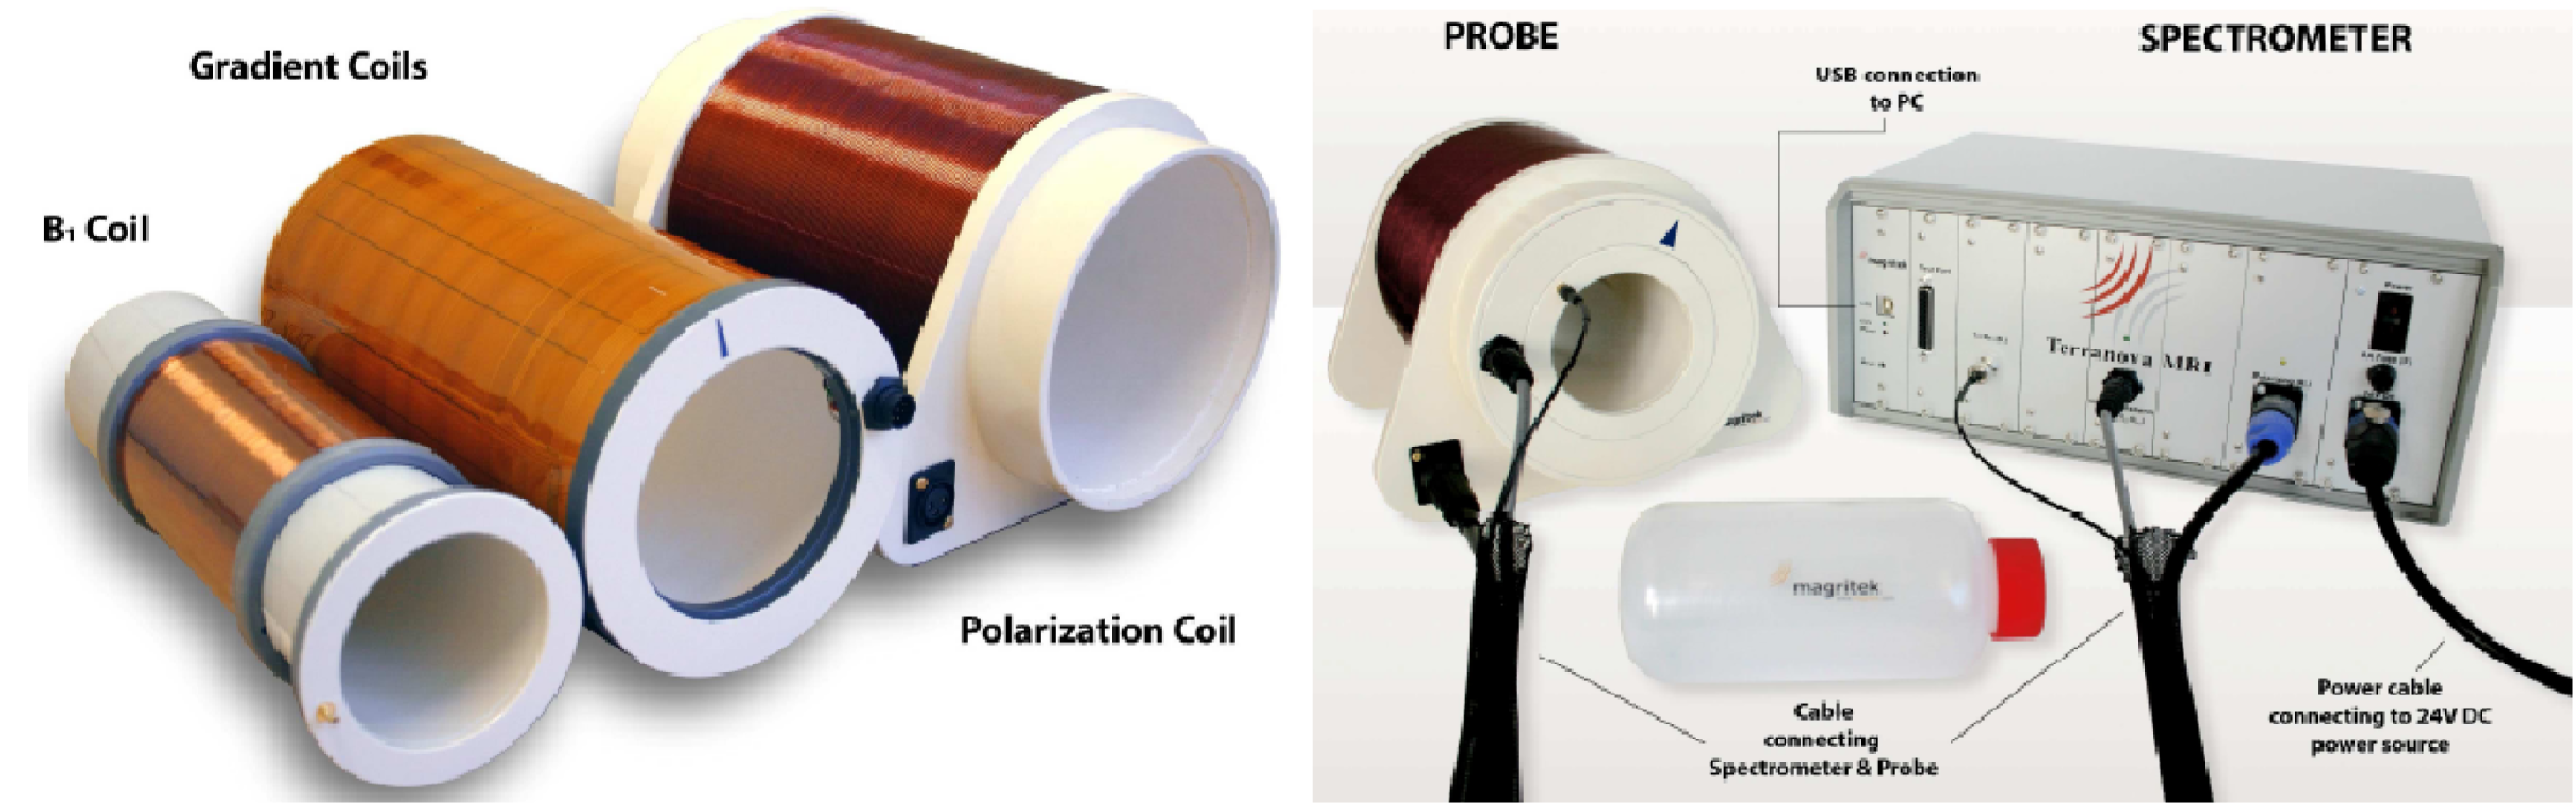
\includegraphics[width= 0.7\textwidth]{Abbildungen/Aufbau.png}   
    \caption[Setup of the \textit{Terranova-MRI EFNMR}. \cite{Bild}]{Setup of the \textit{Terranova-MRI EFNMR}.
    On the left-hand side the coils B$_1$ (excitation and collection coil), gradient coil (homogeneous magnetic field and 2D scanning coil) and the prepolarising coil B$_p$ are displayed.
    The right-hand side shows the water sample which has been used and the spectrometer which adjusts the necessary signals to the coils. \cite{Bild}}
    \label{fig:Aufbau}
\end{figure}
% !!!!!!!!
% !!!!!!!!!!
% !!!!!!!!!
% %Einstellen von größe des Bidles mit epslatex:  \resizebox{0.5\textwidth}{!}{\input{plots/Belichtungszeit.tex}}
% !!!!!!!!!!
% !!!!!!!!!!!
% !!!!!!!!!
\newpage
%----------------------------------------------------------------%
%----------------------Auswertung--------------------------------%
%----------------------------------------------------------------%
% !TEX root = main.tex
\subsection{Noise measurement}
\label{sec:Noisemeasurement}
The first step in the EFNMR Remote experiment is to measure the external noise.
The external noise depends on the location where the setup is placed, the orientation of the probe and on surrounding metal objects e.g. a metal desk.
To detect this external noise, a measurement without an NMR signal is provided.
The time domain noise signal is shown in figure \ref{fig: noise}.
It is clearly visible that the noise is centered around \SI{0}{\mu \volt}.
To gain knowledge about the noise level, the computer calculates the root-mean-square (RMS).
This means that it calculates the square of each data point, then sums up all the squared values, calculates the average and then applies a square root.
With this method the noise level can be calculated.
In this case it has a value of \SI{7.5}{\mu \volt}.
This is of an acceptable magnitude because any value below \SI{10}{\mu \volt} is good enough to provide meaningful NMR data.

\begin{figure}[H]
    \centering
    % GNUPLOT: LaTeX picture with Postscript
\begingroup
  % Encoding inside the plot.  In the header of your document, this encoding
  % should to defined, e.g., by using
  % \usepackage[cp1252,<other encodings>]{inputenc}
  \inputencoding{cp1252}%
  \makeatletter
  \providecommand\color[2][]{%
    \GenericError{(gnuplot) \space\space\space\@spaces}{%
      Package color not loaded in conjunction with
      terminal option `colourtext'%
    }{See the gnuplot documentation for explanation.%
    }{Either use 'blacktext' in gnuplot or load the package
      color.sty in LaTeX.}%
    \renewcommand\color[2][]{}%
  }%
  \providecommand\includegraphics[2][]{%
    \GenericError{(gnuplot) \space\space\space\@spaces}{%
      Package graphicx or graphics not loaded%
    }{See the gnuplot documentation for explanation.%
    }{The gnuplot epslatex terminal needs graphicx.sty or graphics.sty.}%
    \renewcommand\includegraphics[2][]{}%
  }%
  \providecommand\rotatebox[2]{#2}%
  \@ifundefined{ifGPcolor}{%
    \newif\ifGPcolor
    \GPcolorfalse
  }{}%
  \@ifundefined{ifGPblacktext}{%
    \newif\ifGPblacktext
    \GPblacktexttrue
  }{}%
  % define a \g@addto@macro without @ in the name:
  \let\gplgaddtomacro\g@addto@macro
  % define empty templates for all commands taking text:
  \gdef\gplbacktext{}%
  \gdef\gplfronttext{}%
  \makeatother
  \ifGPblacktext
    % no textcolor at all
    \def\colorrgb#1{}%
    \def\colorgray#1{}%
  \else
    % gray or color?
    \ifGPcolor
      \def\colorrgb#1{\color[rgb]{#1}}%
      \def\colorgray#1{\color[gray]{#1}}%
      \expandafter\def\csname LTw\endcsname{\color{white}}%
      \expandafter\def\csname LTb\endcsname{\color{black}}%
      \expandafter\def\csname LTa\endcsname{\color{black}}%
      \expandafter\def\csname LT0\endcsname{\color[rgb]{1,0,0}}%
      \expandafter\def\csname LT1\endcsname{\color[rgb]{0,1,0}}%
      \expandafter\def\csname LT2\endcsname{\color[rgb]{0,0,1}}%
      \expandafter\def\csname LT3\endcsname{\color[rgb]{1,0,1}}%
      \expandafter\def\csname LT4\endcsname{\color[rgb]{0,1,1}}%
      \expandafter\def\csname LT5\endcsname{\color[rgb]{1,1,0}}%
      \expandafter\def\csname LT6\endcsname{\color[rgb]{0,0,0}}%
      \expandafter\def\csname LT7\endcsname{\color[rgb]{1,0.3,0}}%
      \expandafter\def\csname LT8\endcsname{\color[rgb]{0.5,0.5,0.5}}%
    \else
      % gray
      \def\colorrgb#1{\color{black}}%
      \def\colorgray#1{\color[gray]{#1}}%
      \expandafter\def\csname LTw\endcsname{\color{white}}%
      \expandafter\def\csname LTb\endcsname{\color{black}}%
      \expandafter\def\csname LTa\endcsname{\color{black}}%
      \expandafter\def\csname LT0\endcsname{\color{black}}%
      \expandafter\def\csname LT1\endcsname{\color{black}}%
      \expandafter\def\csname LT2\endcsname{\color{black}}%
      \expandafter\def\csname LT3\endcsname{\color{black}}%
      \expandafter\def\csname LT4\endcsname{\color{black}}%
      \expandafter\def\csname LT5\endcsname{\color{black}}%
      \expandafter\def\csname LT6\endcsname{\color{black}}%
      \expandafter\def\csname LT7\endcsname{\color{black}}%
      \expandafter\def\csname LT8\endcsname{\color{black}}%
    \fi
  \fi
    \setlength{\unitlength}{0.0500bp}%
    \ifx\gptboxheight\undefined%
      \newlength{\gptboxheight}%
      \newlength{\gptboxwidth}%
      \newsavebox{\gptboxtext}%
    \fi%
    \setlength{\fboxrule}{0.5pt}%
    \setlength{\fboxsep}{1pt}%
\begin{picture}(7200.00,5040.00)%
    \gplgaddtomacro\gplbacktext{%
      \csname LTb\endcsname%%
      \put(814,704){\makebox(0,0)[r]{\strut{}$-80$}}%
      \put(814,1218){\makebox(0,0)[r]{\strut{}$-60$}}%
      \put(814,1733){\makebox(0,0)[r]{\strut{}$-40$}}%
      \put(814,2247){\makebox(0,0)[r]{\strut{}$-20$}}%
      \put(814,2762){\makebox(0,0)[r]{\strut{}$0$}}%
      \put(814,3276){\makebox(0,0)[r]{\strut{}$20$}}%
      \put(814,3790){\makebox(0,0)[r]{\strut{}$40$}}%
      \put(814,4305){\makebox(0,0)[r]{\strut{}$60$}}%
      \put(814,4819){\makebox(0,0)[r]{\strut{}$80$}}%
      \put(946,484){\makebox(0,0){\strut{}$0$}}%
      \put(1727,484){\makebox(0,0){\strut{}$0.2$}}%
      \put(2508,484){\makebox(0,0){\strut{}$0.4$}}%
      \put(3289,484){\makebox(0,0){\strut{}$0.6$}}%
      \put(4070,484){\makebox(0,0){\strut{}$0.8$}}%
      \put(4851,484){\makebox(0,0){\strut{}$1$}}%
      \put(5632,484){\makebox(0,0){\strut{}$1.2$}}%
      \put(6413,484){\makebox(0,0){\strut{}$1.4$}}%
    }%
    \gplgaddtomacro\gplfronttext{%
      \csname LTb\endcsname%%
      \put(209,2761){\rotatebox{-270}{\makebox(0,0){\strut{}Amplitude in $\si{\mu \volt}$}}}%
      \put(3874,154){\makebox(0,0){\strut{}Time in $\si{\second}$}}%
      \csname LTb\endcsname%%
      \put(5816,4646){\makebox(0,0)[r]{\strut{}noise signal}}%
    }%
    \gplbacktext
    \put(0,0){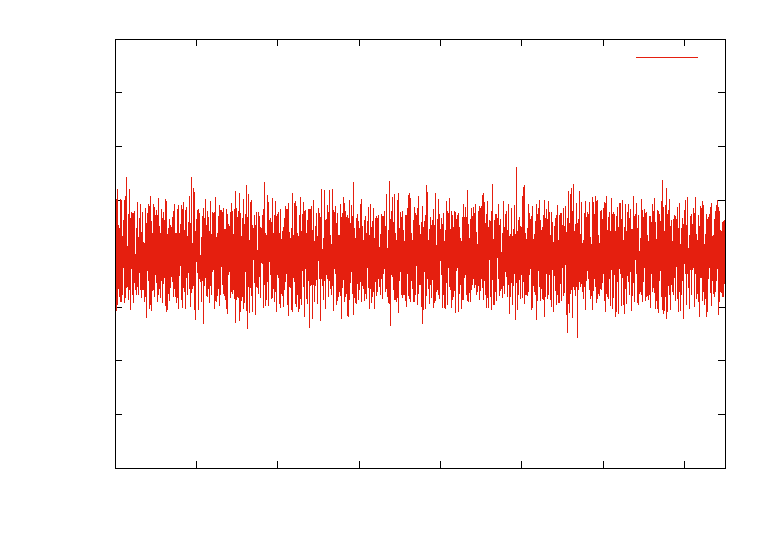
\includegraphics{plots/noise}}%
    \gplfronttext
  \end{picture}%
\endgroup

    \caption[Noise signal taken by the B$_1$ coil.]{Noise signal taken by the B$_1$ coil.
    The noise value of this signal is \SI{7.5}{\mu \volt}.}
    \label{fig: noise}
\end{figure}

Figure \ref{fig: MonitorNoise138} shows the frequency domain noise.
This means that the time domain is fourier transformed into the frequency domain.
This method is one of the basic principles used in this experiment to make research about the properties of the measured signals.
The frequency domain noise shows very specific sharp peaks every \SI{50}{\hertz} interval.
To be more precise the peaks in the middle of every hundred \si{\hertz} step are way higher than those at \SI{1400}{\hertz}, \SI{1500}{\hertz} and so on.
This results from the frequency in the power grid which is \SI{50}{\hertz} in Germany and can also be affiliated to the electrical noise of a surrounding fluorescent light or the CRT computer monitor.
Unfortunately the remote camera program of the computer did not work and therefore it is not clear if there was a fluorescent light in the room.
Even though the noise peaks in the frequency domain figure \ref{fig: MonitorNoise138} indicate that there could be a fluorescent light source in the room.
Despite all sharp peaks, there is also a slight increase of the amplitude around $\SI{185 \pm 10 e1}{\frac{\mu \volt}{\hertz}}$ visible.
This is explicable by the resonance frequency of the instrument and its sensitvity around the larmor frequency (\SI{1841.4}{\hertz} for water in Germany on July 2020).
All our following measurements will be done nearby the larmor frequency.
That is the reason why the instrument sensitvity is sharpend around this value.

\begin{figure}[H]
    \centering
    % GNUPLOT: LaTeX picture with Postscript
\begingroup
  % Encoding inside the plot.  In the header of your document, this encoding
  % should to defined, e.g., by using
  % \usepackage[cp1252,<other encodings>]{inputenc}
  \inputencoding{cp1252}%
  \makeatletter
  \providecommand\color[2][]{%
    \GenericError{(gnuplot) \space\space\space\@spaces}{%
      Package color not loaded in conjunction with
      terminal option `colourtext'%
    }{See the gnuplot documentation for explanation.%
    }{Either use 'blacktext' in gnuplot or load the package
      color.sty in LaTeX.}%
    \renewcommand\color[2][]{}%
  }%
  \providecommand\includegraphics[2][]{%
    \GenericError{(gnuplot) \space\space\space\@spaces}{%
      Package graphicx or graphics not loaded%
    }{See the gnuplot documentation for explanation.%
    }{The gnuplot epslatex terminal needs graphicx.sty or graphics.sty.}%
    \renewcommand\includegraphics[2][]{}%
  }%
  \providecommand\rotatebox[2]{#2}%
  \@ifundefined{ifGPcolor}{%
    \newif\ifGPcolor
    \GPcolorfalse
  }{}%
  \@ifundefined{ifGPblacktext}{%
    \newif\ifGPblacktext
    \GPblacktexttrue
  }{}%
  % define a \g@addto@macro without @ in the name:
  \let\gplgaddtomacro\g@addto@macro
  % define empty templates for all commands taking text:
  \gdef\gplbacktext{}%
  \gdef\gplfronttext{}%
  \makeatother
  \ifGPblacktext
    % no textcolor at all
    \def\colorrgb#1{}%
    \def\colorgray#1{}%
  \else
    % gray or color?
    \ifGPcolor
      \def\colorrgb#1{\color[rgb]{#1}}%
      \def\colorgray#1{\color[gray]{#1}}%
      \expandafter\def\csname LTw\endcsname{\color{white}}%
      \expandafter\def\csname LTb\endcsname{\color{black}}%
      \expandafter\def\csname LTa\endcsname{\color{black}}%
      \expandafter\def\csname LT0\endcsname{\color[rgb]{1,0,0}}%
      \expandafter\def\csname LT1\endcsname{\color[rgb]{0,1,0}}%
      \expandafter\def\csname LT2\endcsname{\color[rgb]{0,0,1}}%
      \expandafter\def\csname LT3\endcsname{\color[rgb]{1,0,1}}%
      \expandafter\def\csname LT4\endcsname{\color[rgb]{0,1,1}}%
      \expandafter\def\csname LT5\endcsname{\color[rgb]{1,1,0}}%
      \expandafter\def\csname LT6\endcsname{\color[rgb]{0,0,0}}%
      \expandafter\def\csname LT7\endcsname{\color[rgb]{1,0.3,0}}%
      \expandafter\def\csname LT8\endcsname{\color[rgb]{0.5,0.5,0.5}}%
    \else
      % gray
      \def\colorrgb#1{\color{black}}%
      \def\colorgray#1{\color[gray]{#1}}%
      \expandafter\def\csname LTw\endcsname{\color{white}}%
      \expandafter\def\csname LTb\endcsname{\color{black}}%
      \expandafter\def\csname LTa\endcsname{\color{black}}%
      \expandafter\def\csname LT0\endcsname{\color{black}}%
      \expandafter\def\csname LT1\endcsname{\color{black}}%
      \expandafter\def\csname LT2\endcsname{\color{black}}%
      \expandafter\def\csname LT3\endcsname{\color{black}}%
      \expandafter\def\csname LT4\endcsname{\color{black}}%
      \expandafter\def\csname LT5\endcsname{\color{black}}%
      \expandafter\def\csname LT6\endcsname{\color{black}}%
      \expandafter\def\csname LT7\endcsname{\color{black}}%
      \expandafter\def\csname LT8\endcsname{\color{black}}%
    \fi
  \fi
    \setlength{\unitlength}{0.0500bp}%
    \ifx\gptboxheight\undefined%
      \newlength{\gptboxheight}%
      \newlength{\gptboxwidth}%
      \newsavebox{\gptboxtext}%
    \fi%
    \setlength{\fboxrule}{0.5pt}%
    \setlength{\fboxsep}{1pt}%
\begin{picture}(7200.00,5040.00)%
    \gplgaddtomacro\gplbacktext{%
      \csname LTb\endcsname%%
      \put(682,704){\makebox(0,0)[r]{\strut{}$0$}}%
      \put(682,1390){\makebox(0,0)[r]{\strut{}$2$}}%
      \put(682,2076){\makebox(0,0)[r]{\strut{}$4$}}%
      \put(682,2762){\makebox(0,0)[r]{\strut{}$6$}}%
      \put(682,3447){\makebox(0,0)[r]{\strut{}$8$}}%
      \put(682,4133){\makebox(0,0)[r]{\strut{}$10$}}%
      \put(682,4819){\makebox(0,0)[r]{\strut{}$12$}}%
      \put(814,484){\makebox(0,0){\strut{}$1400$}}%
      \put(1479,484){\makebox(0,0){\strut{}$1500$}}%
      \put(2145,484){\makebox(0,0){\strut{}$1600$}}%
      \put(2810,484){\makebox(0,0){\strut{}$1700$}}%
      \put(3476,484){\makebox(0,0){\strut{}$1800$}}%
      \put(4141,484){\makebox(0,0){\strut{}$1900$}}%
      \put(4807,484){\makebox(0,0){\strut{}$2000$}}%
      \put(5472,484){\makebox(0,0){\strut{}$2100$}}%
      \put(6138,484){\makebox(0,0){\strut{}$2200$}}%
      \put(6803,484){\makebox(0,0){\strut{}$2300$}}%
    }%
    \gplgaddtomacro\gplfronttext{%
      \csname LTb\endcsname%%
      \put(308,2761){\rotatebox{-270}{\makebox(0,0){\strut{}Amplitude in $\si{\frac{\mu \volt}{\hertz}}$}}}%
      \put(3808,154){\makebox(0,0){\strut{}Frequency in $\si{\hertz}$}}%
      \csname LTb\endcsname%%
      \put(5816,4646){\makebox(0,0)[r]{\strut{}noise magnitude spectrum}}%
    }%
    \gplbacktext
    \put(0,0){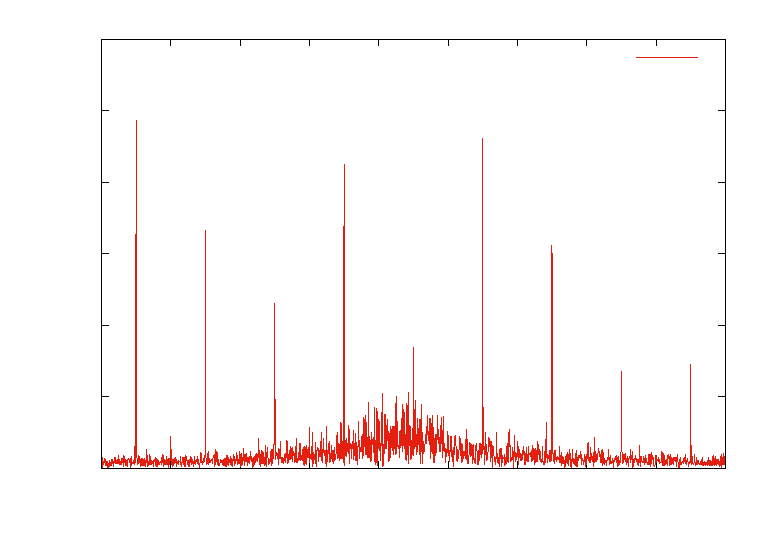
\includegraphics{plots/MonitorNoise138}}%
    \gplfronttext
  \end{picture}%
\endgroup

    \caption[Fourier transformed noise signal of the previous figure \ref{fig: noise}.]{Fourier transformed noise signal of the previous figure \ref{fig: noise}.
    Strong peaks every \SI{50}{\hertz} correspond to the frequency of the power grid in Germany and to electrical noise of a surrounding fluorescent light or the CRT computer monitor.
    The slight increase of the amplitude around $\SI{185 \pm 10}{\cdot 10^1 \frac{\mu \volt}{\hertz}}$ is explicable by the resonance frequency of instrument and its sensitvity around the larmor frequency (\SI{1841.4}{\hertz} for water in Germany in July 2020).}
    \label{fig: MonitorNoise138}
\end{figure}
% !TEX root = main.tex
\section{Coil Analysis}
\label{sec:CoilAnalyssis}
Now knowing that we have an acceptable noise value of less than \SI{10}{\mu \volt}, we can analyse the coil.
In order to do so we explain the general approach of NMR signals first.
To measure a NMR signal a pulse and collect measurement has to be done.
Therefore the B$_1$ coil (transmit and collect coil) has to apply a pulse.
This pulse changes the spins direction out of its thermal equilibrium (along z-axes, due to the earths magnetic field B$_e$) into a direction with a component in the transversal plain.
Therefore the B$_1$ coil collects a signal because it is aligned orthogonal to B$_e$.
The transmit and collect procedure is based on \textsc{Faraday}'s law of induction.
Figure \ref{fig: PulsandcollectValesignal} exemplary shows such a pulse and collect signal by the B$_1$ coil.
Every following measurement in this report is based on the procedure of pulse and collect.

\begin{figure}[H]
    \centering
    % GNUPLOT: LaTeX picture with Postscript
\begingroup
  % Encoding inside the plot.  In the header of your document, this encoding
  % should to defined, e.g., by using
  % \usepackage[cp1252,<other encodings>]{inputenc}
  \inputencoding{cp1252}%
  \makeatletter
  \providecommand\color[2][]{%
    \GenericError{(gnuplot) \space\space\space\@spaces}{%
      Package color not loaded in conjunction with
      terminal option `colourtext'%
    }{See the gnuplot documentation for explanation.%
    }{Either use 'blacktext' in gnuplot or load the package
      color.sty in LaTeX.}%
    \renewcommand\color[2][]{}%
  }%
  \providecommand\includegraphics[2][]{%
    \GenericError{(gnuplot) \space\space\space\@spaces}{%
      Package graphicx or graphics not loaded%
    }{See the gnuplot documentation for explanation.%
    }{The gnuplot epslatex terminal needs graphicx.sty or graphics.sty.}%
    \renewcommand\includegraphics[2][]{}%
  }%
  \providecommand\rotatebox[2]{#2}%
  \@ifundefined{ifGPcolor}{%
    \newif\ifGPcolor
    \GPcolorfalse
  }{}%
  \@ifundefined{ifGPblacktext}{%
    \newif\ifGPblacktext
    \GPblacktexttrue
  }{}%
  % define a \g@addto@macro without @ in the name:
  \let\gplgaddtomacro\g@addto@macro
  % define empty templates for all commands taking text:
  \gdef\gplbacktext{}%
  \gdef\gplfronttext{}%
  \makeatother
  \ifGPblacktext
    % no textcolor at all
    \def\colorrgb#1{}%
    \def\colorgray#1{}%
  \else
    % gray or color?
    \ifGPcolor
      \def\colorrgb#1{\color[rgb]{#1}}%
      \def\colorgray#1{\color[gray]{#1}}%
      \expandafter\def\csname LTw\endcsname{\color{white}}%
      \expandafter\def\csname LTb\endcsname{\color{black}}%
      \expandafter\def\csname LTa\endcsname{\color{black}}%
      \expandafter\def\csname LT0\endcsname{\color[rgb]{1,0,0}}%
      \expandafter\def\csname LT1\endcsname{\color[rgb]{0,1,0}}%
      \expandafter\def\csname LT2\endcsname{\color[rgb]{0,0,1}}%
      \expandafter\def\csname LT3\endcsname{\color[rgb]{1,0,1}}%
      \expandafter\def\csname LT4\endcsname{\color[rgb]{0,1,1}}%
      \expandafter\def\csname LT5\endcsname{\color[rgb]{1,1,0}}%
      \expandafter\def\csname LT6\endcsname{\color[rgb]{0,0,0}}%
      \expandafter\def\csname LT7\endcsname{\color[rgb]{1,0.3,0}}%
      \expandafter\def\csname LT8\endcsname{\color[rgb]{0.5,0.5,0.5}}%
    \else
      % gray
      \def\colorrgb#1{\color{black}}%
      \def\colorgray#1{\color[gray]{#1}}%
      \expandafter\def\csname LTw\endcsname{\color{white}}%
      \expandafter\def\csname LTb\endcsname{\color{black}}%
      \expandafter\def\csname LTa\endcsname{\color{black}}%
      \expandafter\def\csname LT0\endcsname{\color{black}}%
      \expandafter\def\csname LT1\endcsname{\color{black}}%
      \expandafter\def\csname LT2\endcsname{\color{black}}%
      \expandafter\def\csname LT3\endcsname{\color{black}}%
      \expandafter\def\csname LT4\endcsname{\color{black}}%
      \expandafter\def\csname LT5\endcsname{\color{black}}%
      \expandafter\def\csname LT6\endcsname{\color{black}}%
      \expandafter\def\csname LT7\endcsname{\color{black}}%
      \expandafter\def\csname LT8\endcsname{\color{black}}%
    \fi
  \fi
    \setlength{\unitlength}{0.0500bp}%
    \ifx\gptboxheight\undefined%
      \newlength{\gptboxheight}%
      \newlength{\gptboxwidth}%
      \newsavebox{\gptboxtext}%
    \fi%
    \setlength{\fboxrule}{0.5pt}%
    \setlength{\fboxsep}{1pt}%
\begin{picture}(7200.00,5040.00)%
    \gplgaddtomacro\gplbacktext{%
      \csname LTb\endcsname%%
      \put(814,704){\makebox(0,0)[r]{\strut{}$-80$}}%
      \put(814,1218){\makebox(0,0)[r]{\strut{}$-60$}}%
      \put(814,1733){\makebox(0,0)[r]{\strut{}$-40$}}%
      \put(814,2247){\makebox(0,0)[r]{\strut{}$-20$}}%
      \put(814,2762){\makebox(0,0)[r]{\strut{}$0$}}%
      \put(814,3276){\makebox(0,0)[r]{\strut{}$20$}}%
      \put(814,3790){\makebox(0,0)[r]{\strut{}$40$}}%
      \put(814,4305){\makebox(0,0)[r]{\strut{}$60$}}%
      \put(814,4819){\makebox(0,0)[r]{\strut{}$80$}}%
      \put(946,484){\makebox(0,0){\strut{}$0$}}%
      \put(1727,484){\makebox(0,0){\strut{}$0.2$}}%
      \put(2508,484){\makebox(0,0){\strut{}$0.4$}}%
      \put(3289,484){\makebox(0,0){\strut{}$0.6$}}%
      \put(4070,484){\makebox(0,0){\strut{}$0.8$}}%
      \put(4851,484){\makebox(0,0){\strut{}$1$}}%
      \put(5632,484){\makebox(0,0){\strut{}$1.2$}}%
      \put(6413,484){\makebox(0,0){\strut{}$1.4$}}%
    }%
    \gplgaddtomacro\gplfronttext{%
      \csname LTb\endcsname%%
      \put(209,2761){\rotatebox{-270}{\makebox(0,0){\strut{}Amplitude in $\si{\mu \volt}$}}}%
      \put(3874,154){\makebox(0,0){\strut{}Time in $\si{\second}$}}%
      \csname LTb\endcsname%%
      \put(5816,4646){\makebox(0,0)[r]{\strut{}FID data}}%
    }%
    \gplbacktext
    \put(0,0){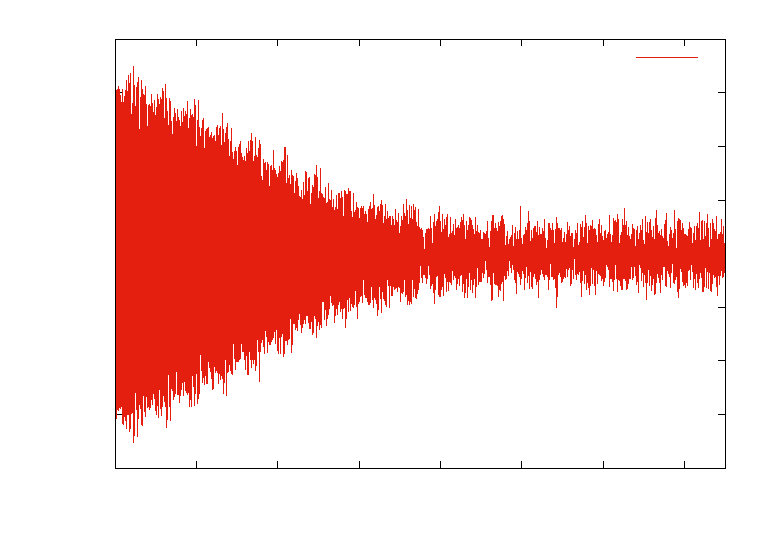
\includegraphics{plots/PulsandcollectValesignal}}%
    \gplfronttext
  \end{picture}%
\endgroup

    \caption[Example signal for a pulse and collect signal made by the B$_1$ coil.]{Example signal for a pulse and collect signal made by the B$_1$ coil.
    The example signal is taken from a FID signal.}
    \label{fig: PulsandcollectValesignal}
\end{figure}

Due to the fact that the B$_1$ coil is a tuned LCR circuit a resonance frequency exists, which can be calculated by the following formula:
\begin{align}
    \omega_{calc} = \frac{1}{\sqrt{L \cdot C}} \ .
    \label{eq: larmorcalc}
\end{align}
In order to analyse the B$_1$ coil the resonance frequency, depending on the capacity, is measured.
Therefore the B$_1$ coil transmits a signal.
Due to this signal the response of the coil can be measured.
This signal is then fourier transformed and the resonance frequency can be deduced from the frequency domain (maximum in the frequency domain).
This procedure is repeated automatically by the computer programm \textit{Prospa} for different capacities.
By changing the capacity we can examine the best capacity in dependence of the larmor frequency.
Figure \ref{fig: Coilanalyse} shows the measured and theoretically calculated resonance frequency (equation \eqref{eq: larmorcalc}; $L = \SI{0.417}{\henry}$) in dependence of the capacity.
The horizontal line represents the larmor frequency of \SI{1841.4}{\hertz} for hydrogen in Germany in July 2020.
To gain this value the vertical component of the earths magnetic field (\SI{43248.8}{\nano \tesla} \cite{magnetfeld}) is multiplied by the gyromagnetic ratio $\SI{42.577}{\frac{\mega \hertz}{\tesla}}$ \cite{magnetfeld}.
The vertical line represents the correct capacity we should use for our measurement, due to the resonance frequency of the larmor frequency.
In this case the correct capacity is \SI{13.8}{\nano \farad}.
Corresponding to the calculated resonance frequency the correct capacity would be \SI{17.9}{\nano \farad}.
It is not deniable that the measured curve is not parallel to the measured resonance frequency.
This probably has its cause in the not fixed inductance $L$.
Due to heating of the coil $L$ might change a little by increasing capacity and thus the calculated curve does not fit to the measured one.
Another reason for the different calculated curve is that we used real coils and those have parasite resistances and also built-in capacities.
This built-in capacity is not taken into account in the formula \eqref{eq: larmorcalc} and therefore the calculated curve might be not correct.
Since the calculated curve does not fit to the measured one, the calculated value for the capacity is not taken into account.

\begin{figure}[H]
    \centering
    % GNUPLOT: LaTeX picture with Postscript
\begingroup
  % Encoding inside the plot.  In the header of your document, this encoding
  % should to defined, e.g., by using
  % \usepackage[cp1252,<other encodings>]{inputenc}
  \inputencoding{cp1252}%
  \makeatletter
  \providecommand\color[2][]{%
    \GenericError{(gnuplot) \space\space\space\@spaces}{%
      Package color not loaded in conjunction with
      terminal option `colourtext'%
    }{See the gnuplot documentation for explanation.%
    }{Either use 'blacktext' in gnuplot or load the package
      color.sty in LaTeX.}%
    \renewcommand\color[2][]{}%
  }%
  \providecommand\includegraphics[2][]{%
    \GenericError{(gnuplot) \space\space\space\@spaces}{%
      Package graphicx or graphics not loaded%
    }{See the gnuplot documentation for explanation.%
    }{The gnuplot epslatex terminal needs graphicx.sty or graphics.sty.}%
    \renewcommand\includegraphics[2][]{}%
  }%
  \providecommand\rotatebox[2]{#2}%
  \@ifundefined{ifGPcolor}{%
    \newif\ifGPcolor
    \GPcolorfalse
  }{}%
  \@ifundefined{ifGPblacktext}{%
    \newif\ifGPblacktext
    \GPblacktexttrue
  }{}%
  % define a \g@addto@macro without @ in the name:
  \let\gplgaddtomacro\g@addto@macro
  % define empty templates for all commands taking text:
  \gdef\gplbacktext{}%
  \gdef\gplfronttext{}%
  \makeatother
  \ifGPblacktext
    % no textcolor at all
    \def\colorrgb#1{}%
    \def\colorgray#1{}%
  \else
    % gray or color?
    \ifGPcolor
      \def\colorrgb#1{\color[rgb]{#1}}%
      \def\colorgray#1{\color[gray]{#1}}%
      \expandafter\def\csname LTw\endcsname{\color{white}}%
      \expandafter\def\csname LTb\endcsname{\color{black}}%
      \expandafter\def\csname LTa\endcsname{\color{black}}%
      \expandafter\def\csname LT0\endcsname{\color[rgb]{1,0,0}}%
      \expandafter\def\csname LT1\endcsname{\color[rgb]{0,1,0}}%
      \expandafter\def\csname LT2\endcsname{\color[rgb]{0,0,1}}%
      \expandafter\def\csname LT3\endcsname{\color[rgb]{1,0,1}}%
      \expandafter\def\csname LT4\endcsname{\color[rgb]{0,1,1}}%
      \expandafter\def\csname LT5\endcsname{\color[rgb]{1,1,0}}%
      \expandafter\def\csname LT6\endcsname{\color[rgb]{0,0,0}}%
      \expandafter\def\csname LT7\endcsname{\color[rgb]{1,0.3,0}}%
      \expandafter\def\csname LT8\endcsname{\color[rgb]{0.5,0.5,0.5}}%
    \else
      % gray
      \def\colorrgb#1{\color{black}}%
      \def\colorgray#1{\color[gray]{#1}}%
      \expandafter\def\csname LTw\endcsname{\color{white}}%
      \expandafter\def\csname LTb\endcsname{\color{black}}%
      \expandafter\def\csname LTa\endcsname{\color{black}}%
      \expandafter\def\csname LT0\endcsname{\color{black}}%
      \expandafter\def\csname LT1\endcsname{\color{black}}%
      \expandafter\def\csname LT2\endcsname{\color{black}}%
      \expandafter\def\csname LT3\endcsname{\color{black}}%
      \expandafter\def\csname LT4\endcsname{\color{black}}%
      \expandafter\def\csname LT5\endcsname{\color{black}}%
      \expandafter\def\csname LT6\endcsname{\color{black}}%
      \expandafter\def\csname LT7\endcsname{\color{black}}%
      \expandafter\def\csname LT8\endcsname{\color{black}}%
    \fi
  \fi
    \setlength{\unitlength}{0.0500bp}%
    \ifx\gptboxheight\undefined%
      \newlength{\gptboxheight}%
      \newlength{\gptboxwidth}%
      \newsavebox{\gptboxtext}%
    \fi%
    \setlength{\fboxrule}{0.5pt}%
    \setlength{\fboxsep}{1pt}%
\begin{picture}(7200.00,5040.00)%
    \gplgaddtomacro\gplbacktext{%
      \csname LTb\endcsname%%
      \put(946,704){\makebox(0,0)[r]{\strut{}$1500$}}%
      \put(946,1527){\makebox(0,0)[r]{\strut{}$2000$}}%
      \put(946,2350){\makebox(0,0)[r]{\strut{}$2500$}}%
      \put(946,3173){\makebox(0,0)[r]{\strut{}$3000$}}%
      \put(946,3996){\makebox(0,0)[r]{\strut{}$3500$}}%
      \put(946,4819){\makebox(0,0)[r]{\strut{}$4000$}}%
      \put(1794,484){\makebox(0,0){\strut{}$6$}}%
      \put(2688,484){\makebox(0,0){\strut{}$8$}}%
      \put(3583,484){\makebox(0,0){\strut{}$10$}}%
      \put(4477,484){\makebox(0,0){\strut{}$12$}}%
      \put(5372,484){\makebox(0,0){\strut{}$14$}}%
      \put(6266,484){\makebox(0,0){\strut{}$16$}}%
    }%
    \gplgaddtomacro\gplfronttext{%
      \csname LTb\endcsname%%
      \put(209,2761){\rotatebox{-270}{\makebox(0,0){\strut{}Frequency $\si{\hertz}$}}}%
      \put(3940,154){\makebox(0,0){\strut{}Capacity in $\si{\nano \farad}$}}%
      \csname LTb\endcsname%%
      \put(5816,4646){\makebox(0,0)[r]{\strut{}measured resonance frequency}}%
      \csname LTb\endcsname%%
      \put(5816,4426){\makebox(0,0)[r]{\strut{}calculated resonance frequency}}%
    }%
    \gplbacktext
    \put(0,0){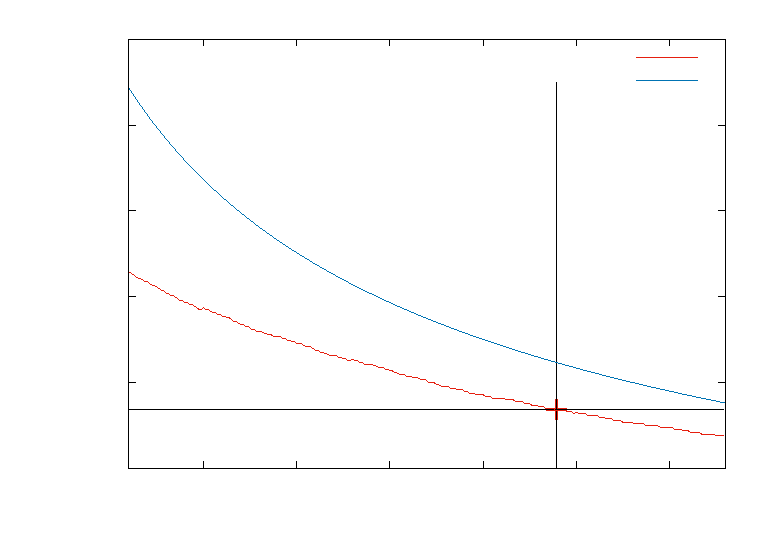
\includegraphics{plots/Coilanalyse}}%
    \gplfronttext
  \end{picture}%
\endgroup

    \caption[This figure shows the measured and calculated resonance frequencies for different capacities.]{This figure shows the measured and calculated resonance frequencies for different capacities.
    The marked cross represents the larmor frequency of \SI{1841.4}{\hertz} for hydrogen in Germany in July 2020.}
    \label{fig: Coilanalyse}
\end{figure}
% !TEX root = main.tex
\section{Optimization and Characterisation of FID in water sample}
\label{sec:OptimizationandCharacterisationofFIDinwatersample}

One of the main goals of this experiment is to measure a good FID of the water sample.
In order to do so we first have to optimize our FID signal of the water probe.\newline
At first the inhomogeneity of the magnetic field has to be cancelled.
The process to make the magnetic field more homogeneous is to \textit{autoshim} the components of the gradient coil.
The computer programm does this automatically. So it de-shims the system step by step and checks if the output maximizes or minimizes.
By checking many different combinations it finds the best shimming values for the gradient coil.
In our case they are:
\begin{align*}
    x &= \SI{10.11}{\milli \ampere}\\
    y &= \SI{20.88}{\milli \ampere}\\
    z &= \SI{-20.07}{\milli \ampere} \ .
    \label{eq: shimmingvalues}
\end{align*}
That means with those shimming values the magnetic field in the setup is as homogeneous as possible.
\\
The second optimization step is to change the B$_1$ pulse duration.
The longer the pulse duration is, the larger is the angle of the flipping spins and thus the signal will get stronger (only for flipping angles up to \SI{90}{\degree}).
The best signal is obtained for a flipping angle of \SI{90}{\degree}, because with this angle the spins only have a component in the transversal plane and therefore the signal is maximized.
If the pulse duration is too long, then the flipping angle is larger than \SI{90}{\degree} and the spins get a horizontal component again and the signal will decrease again.
When a flipping angle of \SI{180}{\degree} is reached the signal will be at its minimum.
Afterwards the signal will rise again, because of the increasing horizontal component.
Figure \ref{fig:B1dauer} shows this issue.
The maxmimum at a pulse duration of \SI{1.35}{\milli \second} is clearly visible.
This means that after applying a B$_1$ pulse with a duration of \SI{1.35}{\milli \second} the spins are in the transversal plane and therefore the best signal is obtained.
\begin{figure}[H]
    \centering
    % GNUPLOT: LaTeX picture with Postscript
\begingroup
  % Encoding inside the plot.  In the header of your document, this encoding
  % should to defined, e.g., by using
  % \usepackage[cp1252,<other encodings>]{inputenc}
  \inputencoding{cp1252}%
  \makeatletter
  \providecommand\color[2][]{%
    \GenericError{(gnuplot) \space\space\space\@spaces}{%
      Package color not loaded in conjunction with
      terminal option `colourtext'%
    }{See the gnuplot documentation for explanation.%
    }{Either use 'blacktext' in gnuplot or load the package
      color.sty in LaTeX.}%
    \renewcommand\color[2][]{}%
  }%
  \providecommand\includegraphics[2][]{%
    \GenericError{(gnuplot) \space\space\space\@spaces}{%
      Package graphicx or graphics not loaded%
    }{See the gnuplot documentation for explanation.%
    }{The gnuplot epslatex terminal needs graphicx.sty or graphics.sty.}%
    \renewcommand\includegraphics[2][]{}%
  }%
  \providecommand\rotatebox[2]{#2}%
  \@ifundefined{ifGPcolor}{%
    \newif\ifGPcolor
    \GPcolorfalse
  }{}%
  \@ifundefined{ifGPblacktext}{%
    \newif\ifGPblacktext
    \GPblacktexttrue
  }{}%
  % define a \g@addto@macro without @ in the name:
  \let\gplgaddtomacro\g@addto@macro
  % define empty templates for all commands taking text:
  \gdef\gplbacktext{}%
  \gdef\gplfronttext{}%
  \makeatother
  \ifGPblacktext
    % no textcolor at all
    \def\colorrgb#1{}%
    \def\colorgray#1{}%
  \else
    % gray or color?
    \ifGPcolor
      \def\colorrgb#1{\color[rgb]{#1}}%
      \def\colorgray#1{\color[gray]{#1}}%
      \expandafter\def\csname LTw\endcsname{\color{white}}%
      \expandafter\def\csname LTb\endcsname{\color{black}}%
      \expandafter\def\csname LTa\endcsname{\color{black}}%
      \expandafter\def\csname LT0\endcsname{\color[rgb]{1,0,0}}%
      \expandafter\def\csname LT1\endcsname{\color[rgb]{0,1,0}}%
      \expandafter\def\csname LT2\endcsname{\color[rgb]{0,0,1}}%
      \expandafter\def\csname LT3\endcsname{\color[rgb]{1,0,1}}%
      \expandafter\def\csname LT4\endcsname{\color[rgb]{0,1,1}}%
      \expandafter\def\csname LT5\endcsname{\color[rgb]{1,1,0}}%
      \expandafter\def\csname LT6\endcsname{\color[rgb]{0,0,0}}%
      \expandafter\def\csname LT7\endcsname{\color[rgb]{1,0.3,0}}%
      \expandafter\def\csname LT8\endcsname{\color[rgb]{0.5,0.5,0.5}}%
    \else
      % gray
      \def\colorrgb#1{\color{black}}%
      \def\colorgray#1{\color[gray]{#1}}%
      \expandafter\def\csname LTw\endcsname{\color{white}}%
      \expandafter\def\csname LTb\endcsname{\color{black}}%
      \expandafter\def\csname LTa\endcsname{\color{black}}%
      \expandafter\def\csname LT0\endcsname{\color{black}}%
      \expandafter\def\csname LT1\endcsname{\color{black}}%
      \expandafter\def\csname LT2\endcsname{\color{black}}%
      \expandafter\def\csname LT3\endcsname{\color{black}}%
      \expandafter\def\csname LT4\endcsname{\color{black}}%
      \expandafter\def\csname LT5\endcsname{\color{black}}%
      \expandafter\def\csname LT6\endcsname{\color{black}}%
      \expandafter\def\csname LT7\endcsname{\color{black}}%
      \expandafter\def\csname LT8\endcsname{\color{black}}%
    \fi
  \fi
    \setlength{\unitlength}{0.0500bp}%
    \ifx\gptboxheight\undefined%
      \newlength{\gptboxheight}%
      \newlength{\gptboxwidth}%
      \newsavebox{\gptboxtext}%
    \fi%
    \setlength{\fboxrule}{0.5pt}%
    \setlength{\fboxsep}{1pt}%
\begin{picture}(7200.00,5040.00)%
    \gplgaddtomacro\gplbacktext{%
      \csname LTb\endcsname%%
      \put(814,704){\makebox(0,0)[r]{\strut{}$60$}}%
      \put(814,1527){\makebox(0,0)[r]{\strut{}$80$}}%
      \put(814,2350){\makebox(0,0)[r]{\strut{}$100$}}%
      \put(814,3173){\makebox(0,0)[r]{\strut{}$120$}}%
      \put(814,3996){\makebox(0,0)[r]{\strut{}$140$}}%
      \put(814,4819){\makebox(0,0)[r]{\strut{}$160$}}%
      \put(946,484){\makebox(0,0){\strut{}$0$}}%
      \put(1678,484){\makebox(0,0){\strut{}$0.5$}}%
      \put(2410,484){\makebox(0,0){\strut{}$1$}}%
      \put(3142,484){\makebox(0,0){\strut{}$1.5$}}%
      \put(3875,484){\makebox(0,0){\strut{}$2$}}%
      \put(4607,484){\makebox(0,0){\strut{}$2.5$}}%
      \put(5339,484){\makebox(0,0){\strut{}$3$}}%
      \put(6071,484){\makebox(0,0){\strut{}$3.5$}}%
      \put(6803,484){\makebox(0,0){\strut{}$4$}}%
    }%
    \gplgaddtomacro\gplfronttext{%
      \csname LTb\endcsname%%
      \put(209,2761){\rotatebox{-270}{\makebox(0,0){\strut{}FID amplitude}}}%
      \put(3874,154){\makebox(0,0){\strut{}$B_1$ pulse in $\si{}{ms}$}}%
      \csname LTb\endcsname%%
      \put(5816,4646){\makebox(0,0)[r]{\strut{}measured resonance amplitude}}%
    }%
    \gplbacktext
    \put(0,0){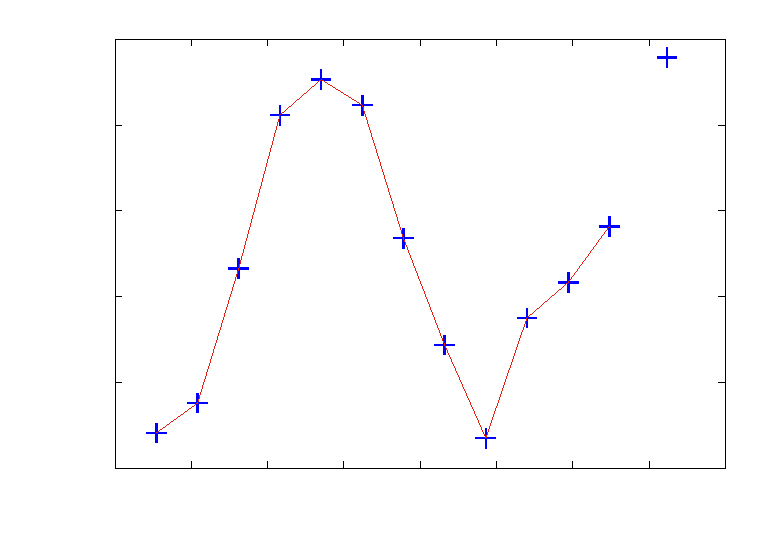
\includegraphics{plots/B1dauer}}%
    \gplfronttext
  \end{picture}%
\endgroup

    \caption[This figure shows which impact the B$_1$ pulse duration has on the amplitude of the FID.]{This figure shows which impact the B$_1$ pulse duration has on the amplitude of the FID.
    It is clearly visible that the duration has a maximum at \SI{1.35}{\milli \second} which is the duration for a \SI{90}{\degree} pulse.}
    \label{fig:B1dauer}
\end{figure}
Figure \ref{fig:pulsedurationbeispiel} exemplary shows the correlation of the B$_1$ pulse duration and the signal which the coil detects.
It is clearly visible that the amplitude is higher for a pulse duration of \SI{1.35}{\milli \second} than for a pulse duration of \SI{0.27}{\milli \second}.
The signal that was taken for the pulse duration of \SI{0.27}{\milli \second} is at the minimum of the figure \ref{fig:B1dauer} and therefore it is correct that the amplitude of the spectrum with the pulse duration of \SI{1.35}{\milli \second} is higher.
\begin{figure}[H]
    \centering
    % GNUPLOT: LaTeX picture with Postscript
\begingroup
  % Encoding inside the plot.  In the header of your document, this encoding
  % should to defined, e.g., by using
  % \usepackage[cp1252,<other encodings>]{inputenc}
  \inputencoding{cp1252}%
  \makeatletter
  \providecommand\color[2][]{%
    \GenericError{(gnuplot) \space\space\space\@spaces}{%
      Package color not loaded in conjunction with
      terminal option `colourtext'%
    }{See the gnuplot documentation for explanation.%
    }{Either use 'blacktext' in gnuplot or load the package
      color.sty in LaTeX.}%
    \renewcommand\color[2][]{}%
  }%
  \providecommand\includegraphics[2][]{%
    \GenericError{(gnuplot) \space\space\space\@spaces}{%
      Package graphicx or graphics not loaded%
    }{See the gnuplot documentation for explanation.%
    }{The gnuplot epslatex terminal needs graphicx.sty or graphics.sty.}%
    \renewcommand\includegraphics[2][]{}%
  }%
  \providecommand\rotatebox[2]{#2}%
  \@ifundefined{ifGPcolor}{%
    \newif\ifGPcolor
    \GPcolorfalse
  }{}%
  \@ifundefined{ifGPblacktext}{%
    \newif\ifGPblacktext
    \GPblacktexttrue
  }{}%
  % define a \g@addto@macro without @ in the name:
  \let\gplgaddtomacro\g@addto@macro
  % define empty templates for all commands taking text:
  \gdef\gplbacktext{}%
  \gdef\gplfronttext{}%
  \makeatother
  \ifGPblacktext
    % no textcolor at all
    \def\colorrgb#1{}%
    \def\colorgray#1{}%
  \else
    % gray or color?
    \ifGPcolor
      \def\colorrgb#1{\color[rgb]{#1}}%
      \def\colorgray#1{\color[gray]{#1}}%
      \expandafter\def\csname LTw\endcsname{\color{white}}%
      \expandafter\def\csname LTb\endcsname{\color{black}}%
      \expandafter\def\csname LTa\endcsname{\color{black}}%
      \expandafter\def\csname LT0\endcsname{\color[rgb]{1,0,0}}%
      \expandafter\def\csname LT1\endcsname{\color[rgb]{0,1,0}}%
      \expandafter\def\csname LT2\endcsname{\color[rgb]{0,0,1}}%
      \expandafter\def\csname LT3\endcsname{\color[rgb]{1,0,1}}%
      \expandafter\def\csname LT4\endcsname{\color[rgb]{0,1,1}}%
      \expandafter\def\csname LT5\endcsname{\color[rgb]{1,1,0}}%
      \expandafter\def\csname LT6\endcsname{\color[rgb]{0,0,0}}%
      \expandafter\def\csname LT7\endcsname{\color[rgb]{1,0.3,0}}%
      \expandafter\def\csname LT8\endcsname{\color[rgb]{0.5,0.5,0.5}}%
    \else
      % gray
      \def\colorrgb#1{\color{black}}%
      \def\colorgray#1{\color[gray]{#1}}%
      \expandafter\def\csname LTw\endcsname{\color{white}}%
      \expandafter\def\csname LTb\endcsname{\color{black}}%
      \expandafter\def\csname LTa\endcsname{\color{black}}%
      \expandafter\def\csname LT0\endcsname{\color{black}}%
      \expandafter\def\csname LT1\endcsname{\color{black}}%
      \expandafter\def\csname LT2\endcsname{\color{black}}%
      \expandafter\def\csname LT3\endcsname{\color{black}}%
      \expandafter\def\csname LT4\endcsname{\color{black}}%
      \expandafter\def\csname LT5\endcsname{\color{black}}%
      \expandafter\def\csname LT6\endcsname{\color{black}}%
      \expandafter\def\csname LT7\endcsname{\color{black}}%
      \expandafter\def\csname LT8\endcsname{\color{black}}%
    \fi
  \fi
    \setlength{\unitlength}{0.0500bp}%
    \ifx\gptboxheight\undefined%
      \newlength{\gptboxheight}%
      \newlength{\gptboxwidth}%
      \newsavebox{\gptboxtext}%
    \fi%
    \setlength{\fboxrule}{0.5pt}%
    \setlength{\fboxsep}{1pt}%
\begin{picture}(7200.00,5040.00)%
    \gplgaddtomacro\gplbacktext{%
      \csname LTb\endcsname%%
      \put(682,704){\makebox(0,0)[r]{\strut{}$0$}}%
      \put(682,1161){\makebox(0,0)[r]{\strut{}$10$}}%
      \put(682,1618){\makebox(0,0)[r]{\strut{}$20$}}%
      \put(682,2076){\makebox(0,0)[r]{\strut{}$30$}}%
      \put(682,2533){\makebox(0,0)[r]{\strut{}$40$}}%
      \put(682,2990){\makebox(0,0)[r]{\strut{}$50$}}%
      \put(682,3447){\makebox(0,0)[r]{\strut{}$60$}}%
      \put(682,3905){\makebox(0,0)[r]{\strut{}$70$}}%
      \put(682,4362){\makebox(0,0)[r]{\strut{}$80$}}%
      \put(682,4819){\makebox(0,0)[r]{\strut{}$90$}}%
      \put(814,484){\makebox(0,0){\strut{}$1800$}}%
      \put(2012,484){\makebox(0,0){\strut{}$1820$}}%
      \put(3210,484){\makebox(0,0){\strut{}$1840$}}%
      \put(4407,484){\makebox(0,0){\strut{}$1860$}}%
      \put(5605,484){\makebox(0,0){\strut{}$1880$}}%
      \put(6803,484){\makebox(0,0){\strut{}$1900$}}%
    }%
    \gplgaddtomacro\gplfronttext{%
      \csname LTb\endcsname%%
      \put(209,2761){\rotatebox{-270}{\makebox(0,0){\strut{}Amplitude in $\si{\mu \volt}$}}}%
      \put(3808,154){\makebox(0,0){\strut{}Frequency in $\si{\hertz}$}}%
      \csname LTb\endcsname%%
      \put(5816,4646){\makebox(0,0)[r]{\strut{}$\SI{0.27}{\milli \second}$ B$_1$ duration}}%
      \csname LTb\endcsname%%
      \put(5816,4426){\makebox(0,0)[r]{\strut{}$\SI{1.35}{\milli \second}$ B$_1$ duration}}%
    }%
    \gplbacktext
    \put(0,0){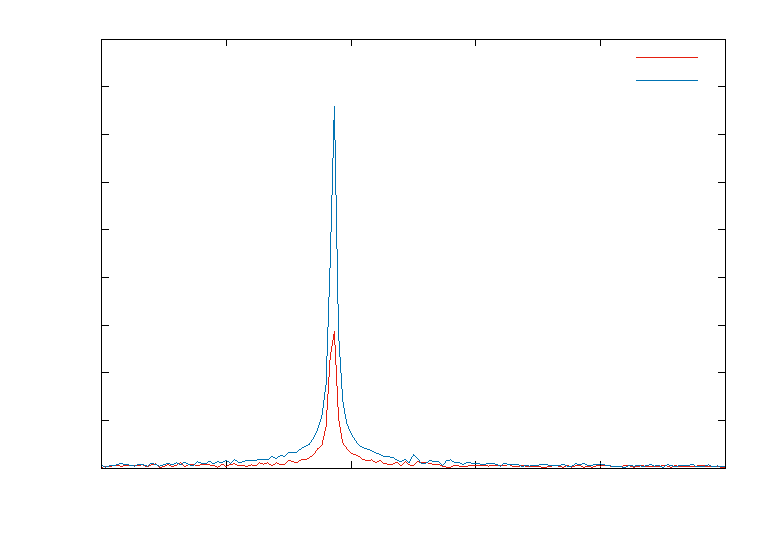
\includegraphics{plots/138_puls_and_collect_number_of_delay25ms_Pulseduration0_27ms}}%
    \gplfronttext
  \end{picture}%
\endgroup

    \caption[Example spectrum for two different B$_1$ pulse durations.]{Example spectrum for two different B$_1$ pulse durations.
    The peak which is higher corresponds to the \SI{1.35}{\milli \second} duration pulse and represents the \SI{90}{\degree} pulse.
    This peak is high, because at this duration most of the spins are in the transversal plane and therfore the amplitude is at its maximum.}
    \label{fig:pulsedurationbeispiel}
\end{figure}
Now that the B$_1$ pulse duration is also optimized, we can have a closer look at the capacity of the LCR circuit of the B$_1$ coil again.
First it is necessary to know that the B$_1$ pulse is applied by a \textit{rectangular} function and the fourier transform of a \textit{rectangular} function is a \textit{sinc} function.
Therefore the fourier transformed spectrum of the B$_1$ pulse signal is a \textit{sinc} function.
When we measure the signal shortly (acquisition delay: \SI{2}{\milli \second}) after the \SI{90}{\degree} pulse, there shoud be a \textit{sinc} function visible and indeed this is what we obtained (figure \ref{fig:Pulsandcollect}).
In figure \ref{fig:Pulsandcollect} there is also a really sharp peak visible.
This is referred to the hydrogen signal.
The hydrogen signal is independed of the applied capacity, but the $B_1$ pulse is, because the capacity changes the properties of the LCR-circuit, of the B$_1$ coil.
The best capacity is adjusted when the hydrogen signal is located in the middle of the \textit{sinc} function, because then the LCR-circuit is tuned to the larmor frequency of the hydrogen signal.
This is also visible by the amplitude of the spectrum in figure \ref{fig:Pulsandcollect}.
The amplitude of the spectrum which was observed for a capacity of \SI{13.8}{\nano \farad} is higher than for the amplitude of the spectrum which was observed for a capacity of \SI{14.2}{\nano \farad}.
As already explained before in chapter \ref{sec:CoilAnalyssis} the capacity of \SI{13.8}{\nano \farad} is indeed the best capacity in order to observe a maximized spectrum.
\begin{figure}[H]
    \centering
    % GNUPLOT: LaTeX picture with Postscript
\begingroup
  % Encoding inside the plot.  In the header of your document, this encoding
  % should to defined, e.g., by using
  % \usepackage[cp1252,<other encodings>]{inputenc}
  \inputencoding{cp1252}%
  \makeatletter
  \providecommand\color[2][]{%
    \GenericError{(gnuplot) \space\space\space\@spaces}{%
      Package color not loaded in conjunction with
      terminal option `colourtext'%
    }{See the gnuplot documentation for explanation.%
    }{Either use 'blacktext' in gnuplot or load the package
      color.sty in LaTeX.}%
    \renewcommand\color[2][]{}%
  }%
  \providecommand\includegraphics[2][]{%
    \GenericError{(gnuplot) \space\space\space\@spaces}{%
      Package graphicx or graphics not loaded%
    }{See the gnuplot documentation for explanation.%
    }{The gnuplot epslatex terminal needs graphicx.sty or graphics.sty.}%
    \renewcommand\includegraphics[2][]{}%
  }%
  \providecommand\rotatebox[2]{#2}%
  \@ifundefined{ifGPcolor}{%
    \newif\ifGPcolor
    \GPcolorfalse
  }{}%
  \@ifundefined{ifGPblacktext}{%
    \newif\ifGPblacktext
    \GPblacktexttrue
  }{}%
  % define a \g@addto@macro without @ in the name:
  \let\gplgaddtomacro\g@addto@macro
  % define empty templates for all commands taking text:
  \gdef\gplbacktext{}%
  \gdef\gplfronttext{}%
  \makeatother
  \ifGPblacktext
    % no textcolor at all
    \def\colorrgb#1{}%
    \def\colorgray#1{}%
  \else
    % gray or color?
    \ifGPcolor
      \def\colorrgb#1{\color[rgb]{#1}}%
      \def\colorgray#1{\color[gray]{#1}}%
      \expandafter\def\csname LTw\endcsname{\color{white}}%
      \expandafter\def\csname LTb\endcsname{\color{black}}%
      \expandafter\def\csname LTa\endcsname{\color{black}}%
      \expandafter\def\csname LT0\endcsname{\color[rgb]{1,0,0}}%
      \expandafter\def\csname LT1\endcsname{\color[rgb]{0,1,0}}%
      \expandafter\def\csname LT2\endcsname{\color[rgb]{0,0,1}}%
      \expandafter\def\csname LT3\endcsname{\color[rgb]{1,0,1}}%
      \expandafter\def\csname LT4\endcsname{\color[rgb]{0,1,1}}%
      \expandafter\def\csname LT5\endcsname{\color[rgb]{1,1,0}}%
      \expandafter\def\csname LT6\endcsname{\color[rgb]{0,0,0}}%
      \expandafter\def\csname LT7\endcsname{\color[rgb]{1,0.3,0}}%
      \expandafter\def\csname LT8\endcsname{\color[rgb]{0.5,0.5,0.5}}%
    \else
      % gray
      \def\colorrgb#1{\color{black}}%
      \def\colorgray#1{\color[gray]{#1}}%
      \expandafter\def\csname LTw\endcsname{\color{white}}%
      \expandafter\def\csname LTb\endcsname{\color{black}}%
      \expandafter\def\csname LTa\endcsname{\color{black}}%
      \expandafter\def\csname LT0\endcsname{\color{black}}%
      \expandafter\def\csname LT1\endcsname{\color{black}}%
      \expandafter\def\csname LT2\endcsname{\color{black}}%
      \expandafter\def\csname LT3\endcsname{\color{black}}%
      \expandafter\def\csname LT4\endcsname{\color{black}}%
      \expandafter\def\csname LT5\endcsname{\color{black}}%
      \expandafter\def\csname LT6\endcsname{\color{black}}%
      \expandafter\def\csname LT7\endcsname{\color{black}}%
      \expandafter\def\csname LT8\endcsname{\color{black}}%
    \fi
  \fi
    \setlength{\unitlength}{0.0500bp}%
    \ifx\gptboxheight\undefined%
      \newlength{\gptboxheight}%
      \newlength{\gptboxwidth}%
      \newsavebox{\gptboxtext}%
    \fi%
    \setlength{\fboxrule}{0.5pt}%
    \setlength{\fboxsep}{1pt}%
\begin{picture}(7200.00,5040.00)%
    \gplgaddtomacro\gplbacktext{%
      \csname LTb\endcsname%%
      \put(814,704){\makebox(0,0)[r]{\strut{}$0$}}%
      \put(814,1390){\makebox(0,0)[r]{\strut{}$20$}}%
      \put(814,2076){\makebox(0,0)[r]{\strut{}$40$}}%
      \put(814,2762){\makebox(0,0)[r]{\strut{}$60$}}%
      \put(814,3447){\makebox(0,0)[r]{\strut{}$80$}}%
      \put(814,4133){\makebox(0,0)[r]{\strut{}$100$}}%
      \put(814,4819){\makebox(0,0)[r]{\strut{}$120$}}%
      \put(946,484){\makebox(0,0){\strut{}$1650$}}%
      \put(1678,484){\makebox(0,0){\strut{}$1700$}}%
      \put(2410,484){\makebox(0,0){\strut{}$1750$}}%
      \put(3142,484){\makebox(0,0){\strut{}$1800$}}%
      \put(3875,484){\makebox(0,0){\strut{}$1850$}}%
      \put(4607,484){\makebox(0,0){\strut{}$1900$}}%
      \put(5339,484){\makebox(0,0){\strut{}$1950$}}%
      \put(6071,484){\makebox(0,0){\strut{}$2000$}}%
      \put(6803,484){\makebox(0,0){\strut{}$2050$}}%
    }%
    \gplgaddtomacro\gplfronttext{%
      \csname LTb\endcsname%%
      \put(209,2761){\rotatebox{-270}{\makebox(0,0){\strut{}Amplitude}}}%
      \put(3874,154){\makebox(0,0){\strut{}Frequency in $\si{\hertz}$}}%
      \csname LTb\endcsname%%
      \put(5816,4646){\makebox(0,0)[r]{\strut{}capacity $\SI{13.8}{\nano \farad}$}}%
      \csname LTb\endcsname%%
      \put(5816,4426){\makebox(0,0)[r]{\strut{}capacity $\SI{14.2}{\nano \farad}$}}%
    }%
    \gplbacktext
    \put(0,0){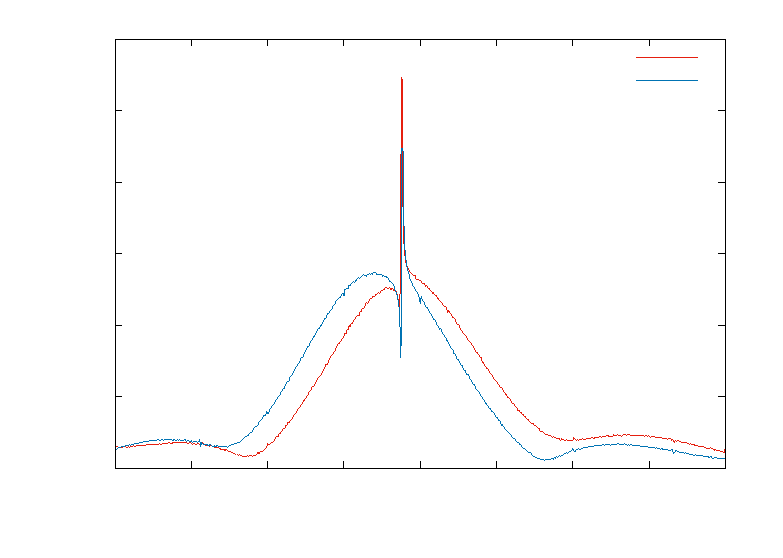
\includegraphics{plots/Pulsandcollect138}}%
    \gplfronttext
  \end{picture}%
\endgroup

    \caption[This figure shows the impact of the capacity in the LCR circuit of the B$_1$ coil.]{This figure shows the impact of the capacity in the LCR circuit of the B$_1$ coil.
    The \textit{sinc} function comes from the fourier transformed B$_1$ pulse, which is rectangular.
    The peak at \SI{1837.27 \pm 0.05}{\hertz} is due to the the hydrogen signal.}
    \label{fig:Pulsandcollect}
\end{figure}
Now that the FID signal is optimized best we can start to characterize it.
Therefore we measure a FID with a acquisition delay of \SI{25}{\milli \second}, because after this delay there are no effects from the rectangular applied B$_1$ pulse anymore (no \textit{sinc} function in the spectrum).
Figure \ref{fig:Pulsandcollect138_delay_25_gauss} shows the observed spectrum and two different fit possibilities.\newline
One option to fit a peak in a spectrum is by applying a \textsc{Voigt} profile ($V(x;\sigma , \gamma)$).
This function is a convolution of the \textsc{Cauchy-Lorentz} and \textsc{Gaussian}distribution and is described by the following formula:
\begin{align}
    V(x;\sigma , \gamma) &= ( G \star L)(x) = \int G(\tau) L(x-\tau) d\tau \\
    G(x;\sigma) &= \frac{exp\left(\frac{-x^2}{2\sigma^2}\right)}{\sigma \sqrt{2 \pi}} \\
    L(x;\gamma)  &= \frac{\gamma}{\pi \left( x^2+\gamma^2\right)} \ .
    \label{eq: voigt} 
\end{align}
The standard deviation is represented by $\sigma$, $\gamma$ specifies the half of the peak width at half height from the \textsc{Lorentz} distribution and $x$ is the shift from the line center.
In figure \ref{fig:Pulsandcollect138_delay_25_gauss} the \textsc{Voigt} profile (green) is fitted to the measured spectrum (red).
The problem of this fit is that it is not as sharp as the measured data.
This might be due to the fact that the measured spectrum does not have many data points especially around the maximum.
Therefore the peak is really sharp and a correct fit with the \textsc{Voigt} profile is rather difficult.
Therefore a second fit function has been applied.
This time only the \textsc{Gaussian} distribution was used.
This fit function is better to calculate the width of the peak, due to the fact that it is easier to fit it to this narrow peak.
The full width of the peak at have maximum (FWHM) is calculated by the applied \textsc{Gaussian} fit and is quantified as \SI{1.177 \pm 0.042}{\hertz}. \newline
The amplitude of the peak is \SI{73.85}{\mu \volt} according to the \textsc{Gaussian} fit and is in comparison to the amplitude of the noise measurement (magnitude \SI{1}{}) in figure \ref{fig: MonitorNoise138} rather high.
The signal to noise ratio of this point is \SI{47.57}{}.
To calculate this value the amplitude at \SI{1837.27}{\hertz} (center of the peak) in figure \ref{fig:Pulsandcollect138_delay_25_gauss} is devided by the value of the amplitude at the same frequency in figure \ref{fig: MonitorNoise138}.
That value clearly shows that the peak must arise from the hydrogen signal and is barely disturbed by any noise.\newline
The width of the measured hydrogen peak at half height (FWHM) is \SI{1.177 \pm 0.042}{\hertz} and hence really sharp.
An even better value can only be achieved by tuning the setup even more.
To show the physical properties, this value is though of a really good size.\newline
The disadvantage of the \textsc{Gaussian} fit is that the area under the curve does not equal the measured one, especially around \SI{1836}{\hertz} and \SI{1839}{\hertz}.
Therefore the discussion of the integral under the measured curve will just be qualitative and will be done in chapter \ref{sec:Hahnecho}.\newline
It is also possible to take a measurement of the imaginary signal of the peak in figure \ref{fig:Pulsandcollect138_delay_25_gauss}.
Unfortunately we did not safe this data.
Beacuse of that we explain what we should see and what it means.
The imaginary component describes the dispersion spectrum.
The spectrum then has to look like a hyperbolic function with the pole exactly at \SI{1837.27}{\hertz} (center of the peak).
Since it is no real hyperbolic function there exist values at the pole.
Those values are aligned in a vertical line.
\begin{figure}[H]
    \centering
    % GNUPLOT: LaTeX picture with Postscript
\begingroup
  % Encoding inside the plot.  In the header of your document, this encoding
  % should to defined, e.g., by using
  % \usepackage[cp1252,<other encodings>]{inputenc}
  \inputencoding{cp1252}%
  \makeatletter
  \providecommand\color[2][]{%
    \GenericError{(gnuplot) \space\space\space\@spaces}{%
      Package color not loaded in conjunction with
      terminal option `colourtext'%
    }{See the gnuplot documentation for explanation.%
    }{Either use 'blacktext' in gnuplot or load the package
      color.sty in LaTeX.}%
    \renewcommand\color[2][]{}%
  }%
  \providecommand\includegraphics[2][]{%
    \GenericError{(gnuplot) \space\space\space\@spaces}{%
      Package graphicx or graphics not loaded%
    }{See the gnuplot documentation for explanation.%
    }{The gnuplot epslatex terminal needs graphicx.sty or graphics.sty.}%
    \renewcommand\includegraphics[2][]{}%
  }%
  \providecommand\rotatebox[2]{#2}%
  \@ifundefined{ifGPcolor}{%
    \newif\ifGPcolor
    \GPcolorfalse
  }{}%
  \@ifundefined{ifGPblacktext}{%
    \newif\ifGPblacktext
    \GPblacktexttrue
  }{}%
  % define a \g@addto@macro without @ in the name:
  \let\gplgaddtomacro\g@addto@macro
  % define empty templates for all commands taking text:
  \gdef\gplbacktext{}%
  \gdef\gplfronttext{}%
  \makeatother
  \ifGPblacktext
    % no textcolor at all
    \def\colorrgb#1{}%
    \def\colorgray#1{}%
  \else
    % gray or color?
    \ifGPcolor
      \def\colorrgb#1{\color[rgb]{#1}}%
      \def\colorgray#1{\color[gray]{#1}}%
      \expandafter\def\csname LTw\endcsname{\color{white}}%
      \expandafter\def\csname LTb\endcsname{\color{black}}%
      \expandafter\def\csname LTa\endcsname{\color{black}}%
      \expandafter\def\csname LT0\endcsname{\color[rgb]{1,0,0}}%
      \expandafter\def\csname LT1\endcsname{\color[rgb]{0,1,0}}%
      \expandafter\def\csname LT2\endcsname{\color[rgb]{0,0,1}}%
      \expandafter\def\csname LT3\endcsname{\color[rgb]{1,0,1}}%
      \expandafter\def\csname LT4\endcsname{\color[rgb]{0,1,1}}%
      \expandafter\def\csname LT5\endcsname{\color[rgb]{1,1,0}}%
      \expandafter\def\csname LT6\endcsname{\color[rgb]{0,0,0}}%
      \expandafter\def\csname LT7\endcsname{\color[rgb]{1,0.3,0}}%
      \expandafter\def\csname LT8\endcsname{\color[rgb]{0.5,0.5,0.5}}%
    \else
      % gray
      \def\colorrgb#1{\color{black}}%
      \def\colorgray#1{\color[gray]{#1}}%
      \expandafter\def\csname LTw\endcsname{\color{white}}%
      \expandafter\def\csname LTb\endcsname{\color{black}}%
      \expandafter\def\csname LTa\endcsname{\color{black}}%
      \expandafter\def\csname LT0\endcsname{\color{black}}%
      \expandafter\def\csname LT1\endcsname{\color{black}}%
      \expandafter\def\csname LT2\endcsname{\color{black}}%
      \expandafter\def\csname LT3\endcsname{\color{black}}%
      \expandafter\def\csname LT4\endcsname{\color{black}}%
      \expandafter\def\csname LT5\endcsname{\color{black}}%
      \expandafter\def\csname LT6\endcsname{\color{black}}%
      \expandafter\def\csname LT7\endcsname{\color{black}}%
      \expandafter\def\csname LT8\endcsname{\color{black}}%
    \fi
  \fi
    \setlength{\unitlength}{0.0500bp}%
    \ifx\gptboxheight\undefined%
      \newlength{\gptboxheight}%
      \newlength{\gptboxwidth}%
      \newsavebox{\gptboxtext}%
    \fi%
    \setlength{\fboxrule}{0.5pt}%
    \setlength{\fboxsep}{1pt}%
\begin{picture}(7200.00,5040.00)%
    \gplgaddtomacro\gplbacktext{%
      \csname LTb\endcsname%%
      \put(682,704){\makebox(0,0)[r]{\strut{}$0$}}%
      \put(682,1161){\makebox(0,0)[r]{\strut{}$10$}}%
      \put(682,1618){\makebox(0,0)[r]{\strut{}$20$}}%
      \put(682,2076){\makebox(0,0)[r]{\strut{}$30$}}%
      \put(682,2533){\makebox(0,0)[r]{\strut{}$40$}}%
      \put(682,2990){\makebox(0,0)[r]{\strut{}$50$}}%
      \put(682,3447){\makebox(0,0)[r]{\strut{}$60$}}%
      \put(682,3905){\makebox(0,0)[r]{\strut{}$70$}}%
      \put(682,4362){\makebox(0,0)[r]{\strut{}$80$}}%
      \put(682,4819){\makebox(0,0)[r]{\strut{}$90$}}%
      \put(814,484){\makebox(0,0){\strut{}$1830$}}%
      \put(1613,484){\makebox(0,0){\strut{}$1832$}}%
      \put(2411,484){\makebox(0,0){\strut{}$1834$}}%
      \put(3210,484){\makebox(0,0){\strut{}$1836$}}%
      \put(4008,484){\makebox(0,0){\strut{}$1838$}}%
      \put(4807,484){\makebox(0,0){\strut{}$1840$}}%
      \put(5605,484){\makebox(0,0){\strut{}$1842$}}%
      \put(6404,484){\makebox(0,0){\strut{}$1844$}}%
      \put(4208,2304){\makebox(0,0)[l]{\strut{}FWHM $= \SI{1.177 \pm 0.042}{\hertz}$}}%
      \put(4208,2762){\makebox(0,0)[l]{\strut{}$\sigma =  \SI{0.500 \pm 0.018}{\hertz}$}}%
    }%
    \gplgaddtomacro\gplfronttext{%
      \csname LTb\endcsname%%
      \put(209,2761){\rotatebox{-270}{\makebox(0,0){\strut{}Amplitude in $\si{\mu \volt}$}}}%
      \put(3808,154){\makebox(0,0){\strut{}Frequency in $\si{\hertz}$}}%
      \csname LTb\endcsname%%
      \put(5816,4646){\makebox(0,0)[r]{\strut{}magnitude spectrum}}%
      \csname LTb\endcsname%%
      \put(5816,4426){\makebox(0,0)[r]{\strut{}voigt-profile}}%
      \csname LTb\endcsname%%
      \put(5816,4206){\makebox(0,0)[r]{\strut{}\textsc{Gauss}-Fit}}%
    }%
    \gplbacktext
    \put(0,0){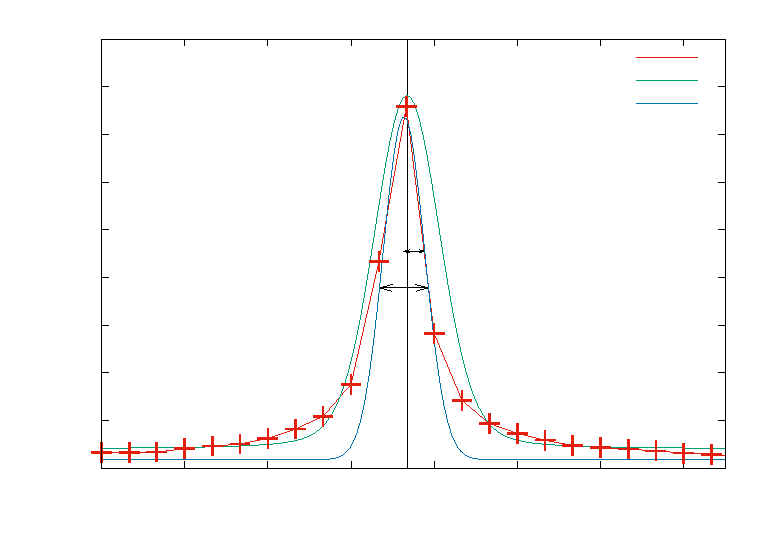
\includegraphics{plots/Pulsandcollect138_delay_25_gauss}}%
    \gplfronttext
  \end{picture}%
\endgroup

    \caption[This figure shows the measured hydrogen signal after an acquisition delay of \SI{25}{\milli \second} and two possible ways to fit the peak.]{This figure shows the measured hydrogen signal after an acquisition delay of \SI{25}{\milli \second} and two possible ways to fit the peak.
    Due to a very short frequency range the peak looks very wide. Indeed it is actually very sharp.
    To fit the peak a \textsc{Voigt} profile and \textsc{Gaussian} fit is used.}
    \label{fig:Pulsandcollect138_delay_25_gauss}
\end{figure}
% !TEX root = main.tex
\section{Longitudinal relaxation measurements T1}
\label{sec:LongitudinalrelaxationmeasurementsT1}
There exist two possibilities to measure the longitudinal spin lattice relaxation.
First we want to have a closer look at the measurement via $\tau_p$ (polarizing pulse duration).
Therefore the computer program \textit{Prospa} applies a polarizing pulse orthogonal to the earths magnetic field.
Due to this polarizing pulse the spins align in the transversal plain and form a bulk magnetization.
By time the magnetization becomes stronger because of this the signal becomes stronger.
This relation is visualized in the figure \ref{fig:BildT1}.

\begin{figure}[H]
    \centering
    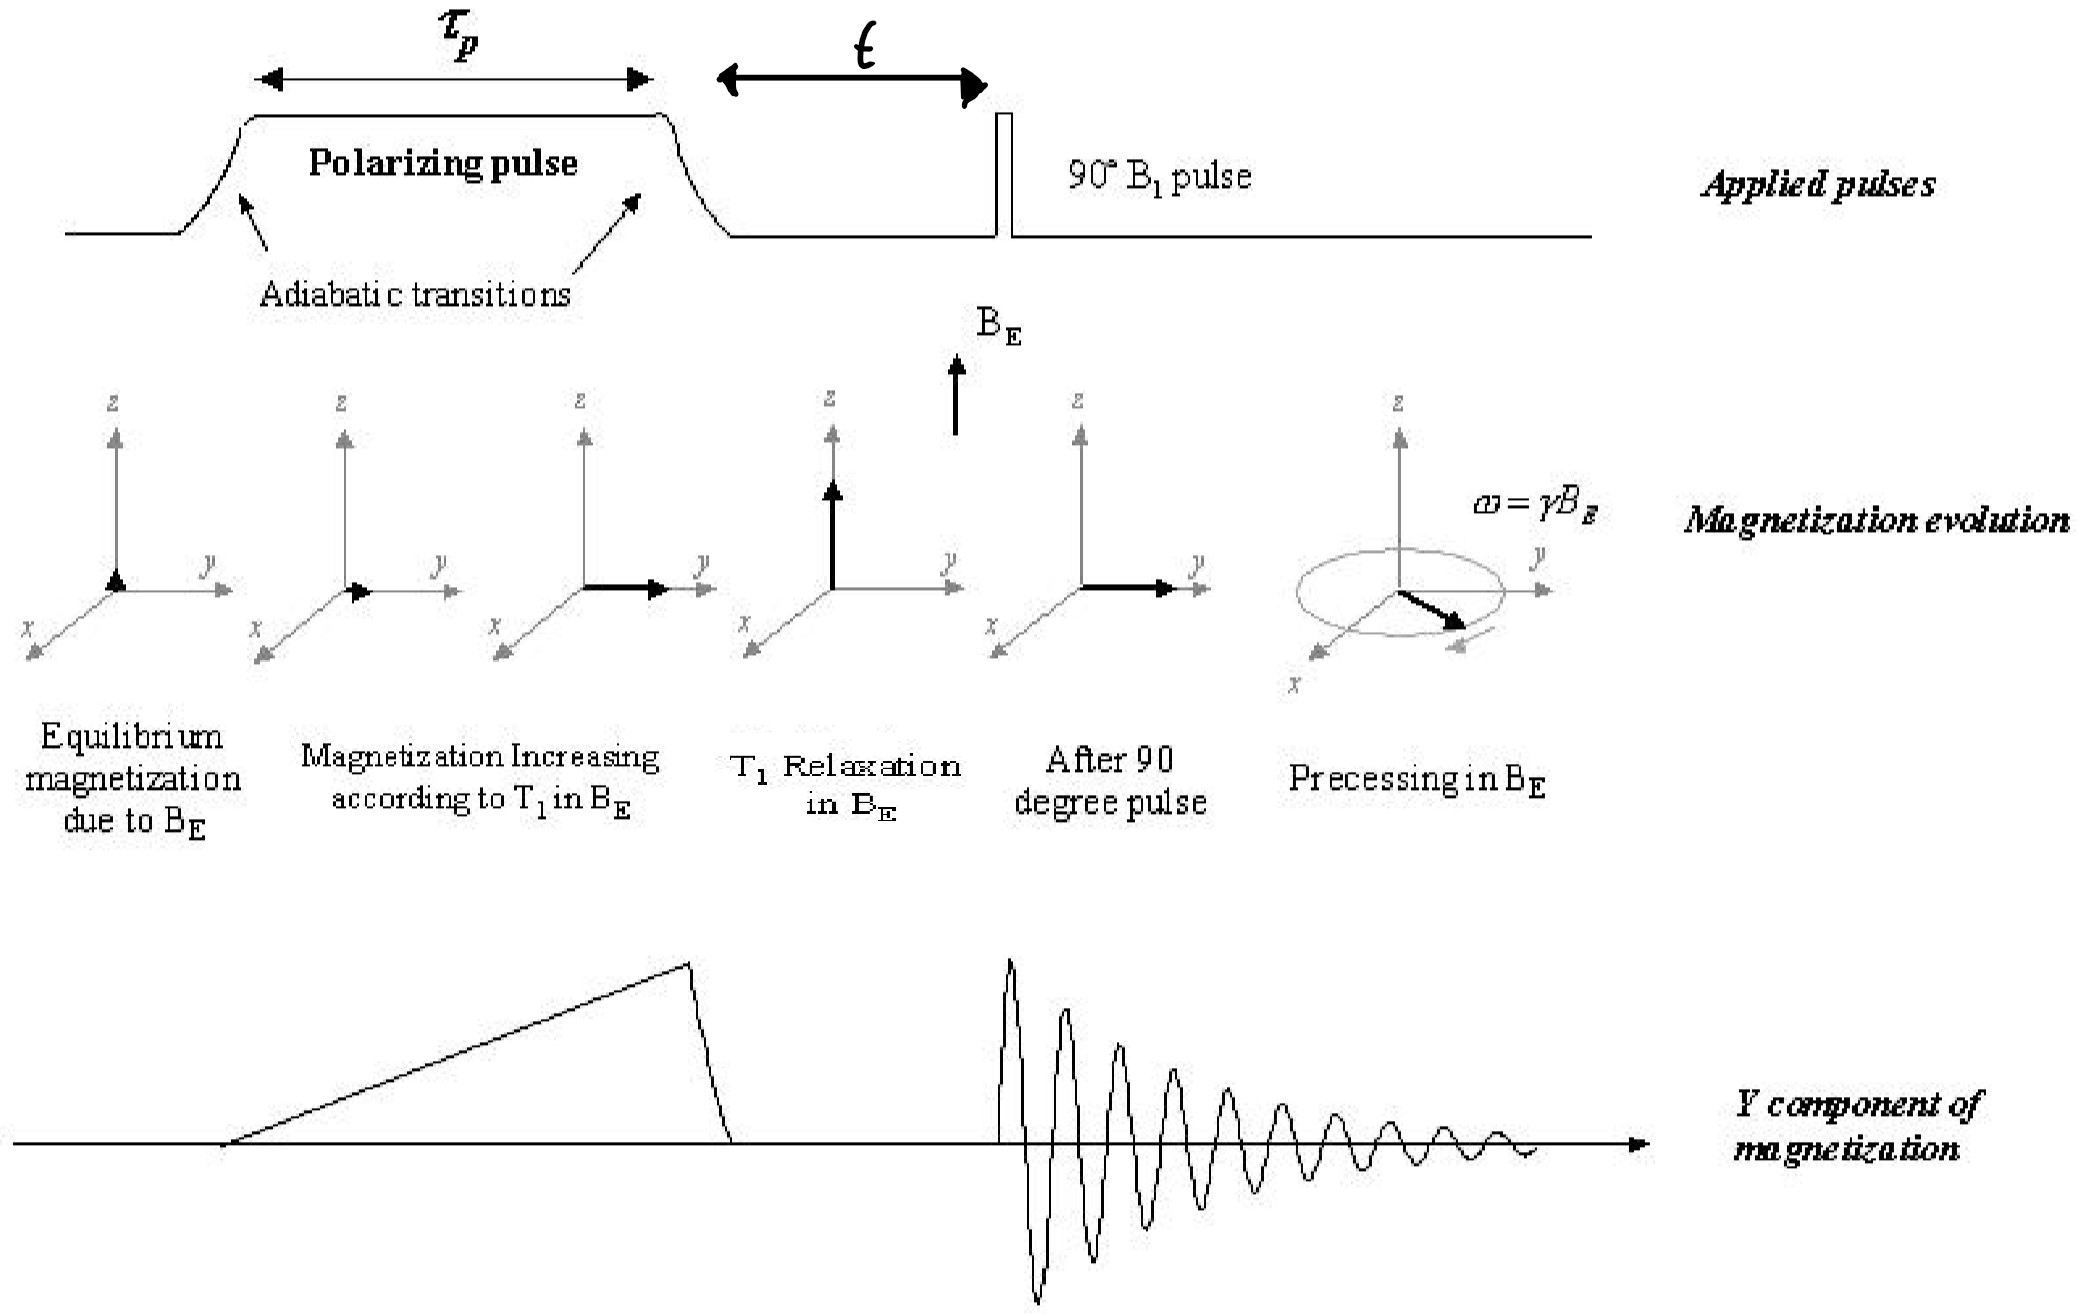
\includegraphics[width= \textwidth]{Abbildungen/BildT1.png}   
    \caption[Sketch to show how $T_1$ can be measured. \cite{Bild}]{Sketch to show how $T_1$ can be measured.
    One way is by changing the polarizing pulse duration $\tau_p$ and the other way is by varying the time between the polarizing pulse and the \SI{90}{\degree} pulse. \cite{Bild}}
    \label{fig:BildT1}
\end{figure}

Due to the increasing magnetization it is possible to calculate the $T_{1,p}$ relaxation.
In order to do so the magnetization time is increased step by step from \SI{500}{\milli \second} to \SI{4500}{\milli \second} with an increment of \SI{500}{\milli \second} and in each configuration the signals maximum is obtained from the fourier transformed spectrum.
Figure \ref{fig:T1Polarisationsfeldfeld} shows the attenuation of the signals normalized to the maximum peak E$_0$.
The underlying idea is that by applying a fit function as following:
\begin{align}
    S(x)=S_0 \cdot \left[1-\exp\left(\frac{-x}{T_{1,p}}\right)\right] \ ,
    \label{eq: fitBp}
\end{align}
it is possible to calculate the relaxation time $T_{1,p}$.
The exponential decay is a result of the loss of phase coherence between the spins and will be used for every measurement of spin relaxation.
In this case $T_{1,p}$ is found to count as \SI{2912.8800 \pm 0.0048}{\milli \second}.

\begin{figure}[H]
    \centering
    % GNUPLOT: LaTeX picture with Postscript
\begingroup
  % Encoding inside the plot.  In the header of your document, this encoding
  % should to defined, e.g., by using
  % \usepackage[cp1252,<other encodings>]{inputenc}
  \inputencoding{cp1252}%
  \makeatletter
  \providecommand\color[2][]{%
    \GenericError{(gnuplot) \space\space\space\@spaces}{%
      Package color not loaded in conjunction with
      terminal option `colourtext'%
    }{See the gnuplot documentation for explanation.%
    }{Either use 'blacktext' in gnuplot or load the package
      color.sty in LaTeX.}%
    \renewcommand\color[2][]{}%
  }%
  \providecommand\includegraphics[2][]{%
    \GenericError{(gnuplot) \space\space\space\@spaces}{%
      Package graphicx or graphics not loaded%
    }{See the gnuplot documentation for explanation.%
    }{The gnuplot epslatex terminal needs graphicx.sty or graphics.sty.}%
    \renewcommand\includegraphics[2][]{}%
  }%
  \providecommand\rotatebox[2]{#2}%
  \@ifundefined{ifGPcolor}{%
    \newif\ifGPcolor
    \GPcolorfalse
  }{}%
  \@ifundefined{ifGPblacktext}{%
    \newif\ifGPblacktext
    \GPblacktexttrue
  }{}%
  % define a \g@addto@macro without @ in the name:
  \let\gplgaddtomacro\g@addto@macro
  % define empty templates for all commands taking text:
  \gdef\gplbacktext{}%
  \gdef\gplfronttext{}%
  \makeatother
  \ifGPblacktext
    % no textcolor at all
    \def\colorrgb#1{}%
    \def\colorgray#1{}%
  \else
    % gray or color?
    \ifGPcolor
      \def\colorrgb#1{\color[rgb]{#1}}%
      \def\colorgray#1{\color[gray]{#1}}%
      \expandafter\def\csname LTw\endcsname{\color{white}}%
      \expandafter\def\csname LTb\endcsname{\color{black}}%
      \expandafter\def\csname LTa\endcsname{\color{black}}%
      \expandafter\def\csname LT0\endcsname{\color[rgb]{1,0,0}}%
      \expandafter\def\csname LT1\endcsname{\color[rgb]{0,1,0}}%
      \expandafter\def\csname LT2\endcsname{\color[rgb]{0,0,1}}%
      \expandafter\def\csname LT3\endcsname{\color[rgb]{1,0,1}}%
      \expandafter\def\csname LT4\endcsname{\color[rgb]{0,1,1}}%
      \expandafter\def\csname LT5\endcsname{\color[rgb]{1,1,0}}%
      \expandafter\def\csname LT6\endcsname{\color[rgb]{0,0,0}}%
      \expandafter\def\csname LT7\endcsname{\color[rgb]{1,0.3,0}}%
      \expandafter\def\csname LT8\endcsname{\color[rgb]{0.5,0.5,0.5}}%
    \else
      % gray
      \def\colorrgb#1{\color{black}}%
      \def\colorgray#1{\color[gray]{#1}}%
      \expandafter\def\csname LTw\endcsname{\color{white}}%
      \expandafter\def\csname LTb\endcsname{\color{black}}%
      \expandafter\def\csname LTa\endcsname{\color{black}}%
      \expandafter\def\csname LT0\endcsname{\color{black}}%
      \expandafter\def\csname LT1\endcsname{\color{black}}%
      \expandafter\def\csname LT2\endcsname{\color{black}}%
      \expandafter\def\csname LT3\endcsname{\color{black}}%
      \expandafter\def\csname LT4\endcsname{\color{black}}%
      \expandafter\def\csname LT5\endcsname{\color{black}}%
      \expandafter\def\csname LT6\endcsname{\color{black}}%
      \expandafter\def\csname LT7\endcsname{\color{black}}%
      \expandafter\def\csname LT8\endcsname{\color{black}}%
    \fi
  \fi
    \setlength{\unitlength}{0.0500bp}%
    \ifx\gptboxheight\undefined%
      \newlength{\gptboxheight}%
      \newlength{\gptboxwidth}%
      \newsavebox{\gptboxtext}%
    \fi%
    \setlength{\fboxrule}{0.5pt}%
    \setlength{\fboxsep}{1pt}%
\begin{picture}(7200.00,5040.00)%
    \gplgaddtomacro\gplbacktext{%
      \csname LTb\endcsname%%
      \put(814,704){\makebox(0,0)[r]{\strut{}$0$}}%
      \put(814,1527){\makebox(0,0)[r]{\strut{}$0.2$}}%
      \put(814,2350){\makebox(0,0)[r]{\strut{}$0.4$}}%
      \put(814,3173){\makebox(0,0)[r]{\strut{}$0.6$}}%
      \put(814,3996){\makebox(0,0)[r]{\strut{}$0.8$}}%
      \put(814,4819){\makebox(0,0)[r]{\strut{}$1$}}%
      \put(946,484){\makebox(0,0){\strut{}$0$}}%
      \put(1660,484){\makebox(0,0){\strut{}$500$}}%
      \put(2375,484){\makebox(0,0){\strut{}$1000$}}%
      \put(3089,484){\makebox(0,0){\strut{}$1500$}}%
      \put(3803,484){\makebox(0,0){\strut{}$2000$}}%
      \put(4517,484){\makebox(0,0){\strut{}$2500$}}%
      \put(5232,484){\makebox(0,0){\strut{}$3000$}}%
      \put(5946,484){\makebox(0,0){\strut{}$3500$}}%
      \put(6660,484){\makebox(0,0){\strut{}$4000$}}%
    }%
    \gplgaddtomacro\gplfronttext{%
      \csname LTb\endcsname%%
      \put(209,2761){\rotatebox{-270}{\makebox(0,0){\strut{}Attenuation $\frac{\text{E}}{\text{E}_0}$}}}%
      \put(3874,154){\makebox(0,0){\strut{}Time in $\si{\milli \second}$}}%
      \csname LTb\endcsname%%
      \put(5816,4646){\makebox(0,0)[r]{\strut{}measured values$ }}%
      \csname LTb\endcsname%%
      \put(5816,4426){\makebox(0,0)[r]{\strut{}attenuation-Fit}}%
    }%
    \gplbacktext
    \put(0,0){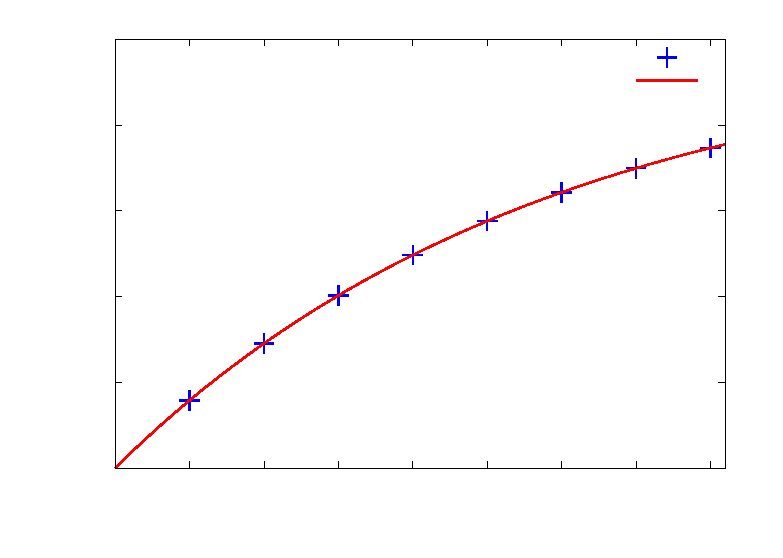
\includegraphics{plots/T1Polarisationsfeldfeld}}%
    \gplfronttext
  \end{picture}%
\endgroup

    \caption[$T_{1,p}$ measurement by varying $\tau_p$ and observing how the attenuation $\frac{\text{E}}{\text{E}_0}$ evolves.]{$T_{1,p}$ measurement by varying $\tau_p$ and observing how the attenuation $\frac{\text{E}}{\text{E}_0}$ evolves.
    The provided exponential fit results in a value for $T_{1,p}$ of \SI{2912.8800 \pm 0.0048}{\milli \second}.}
    \label{fig:T1Polarisationsfeldfeld}
\end{figure}

The second option is to calculate the spin lattice relaxation via the earths magnetic field B$_e$.
In this case the index will be chosen as "$e$" for the spin lattice relaxation.
The procedure in this case is to change the time $t$ (pre-90 minimum delay) between the polarizing pulse ends and the \SI{90}{\degree} pulse begins.
This relation is also visualized in figure \ref{fig:BildT1}.
The pre-90 minimum delay is chosen as \SI{0}{\milli \second} and the pre-90 delay step size as \SI{500}{\milli \second}.
For every configuration the signal maximum is calculated again of the fourier transformed spectrum.
Figure \ref{fig:T1Erdmagnetfeld} shows the attenuation of the signals normalized to the maximum peak E$_0$.
This time the $T_{1,e}$ can be calculated by the following fit function:
\begin{align}
    S(x) = S_0 \cdot \exp\left(\frac{-x}{T_{1,e}}\right) \ .
    \label{eq: fitBe}
\end{align}
In our case $T_{1,e}$ is observed to be \SI{2753.0500 \pm 0.0012}{\milli \second}.\newline
In both ways the uncertainty of the $T_1$ values are quite small.
This is the result of really good aligned values to the fit function.
Nevertheless $T_{1,p}$ and $T_{1,e}$ are not consistent even though the uncertainty is considered.
This might be, due to the fact that those two measurements are based on two different methods and $T_{1,e}$ is dependent on the earths magnetic field.
Even though they are not consistent, the values for $T_{1,p}$ and $T_{1,e}$ have the same magnitude and also have the same magnitude according to a literature value of \SI{4000}{\milli \second} \cite{literaturT1}.
It is good to keep in mind that a comparison to literature values is just there to get the magnitude.
Since the surrounding magnetic field and the probe define the exact value.
\begin{figure}[H]
    \centering
    % GNUPLOT: LaTeX picture with Postscript
\begingroup
  % Encoding inside the plot.  In the header of your document, this encoding
  % should to defined, e.g., by using
  % \usepackage[cp1252,<other encodings>]{inputenc}
  \inputencoding{cp1252}%
  \makeatletter
  \providecommand\color[2][]{%
    \GenericError{(gnuplot) \space\space\space\@spaces}{%
      Package color not loaded in conjunction with
      terminal option `colourtext'%
    }{See the gnuplot documentation for explanation.%
    }{Either use 'blacktext' in gnuplot or load the package
      color.sty in LaTeX.}%
    \renewcommand\color[2][]{}%
  }%
  \providecommand\includegraphics[2][]{%
    \GenericError{(gnuplot) \space\space\space\@spaces}{%
      Package graphicx or graphics not loaded%
    }{See the gnuplot documentation for explanation.%
    }{The gnuplot epslatex terminal needs graphicx.sty or graphics.sty.}%
    \renewcommand\includegraphics[2][]{}%
  }%
  \providecommand\rotatebox[2]{#2}%
  \@ifundefined{ifGPcolor}{%
    \newif\ifGPcolor
    \GPcolorfalse
  }{}%
  \@ifundefined{ifGPblacktext}{%
    \newif\ifGPblacktext
    \GPblacktexttrue
  }{}%
  % define a \g@addto@macro without @ in the name:
  \let\gplgaddtomacro\g@addto@macro
  % define empty templates for all commands taking text:
  \gdef\gplbacktext{}%
  \gdef\gplfronttext{}%
  \makeatother
  \ifGPblacktext
    % no textcolor at all
    \def\colorrgb#1{}%
    \def\colorgray#1{}%
  \else
    % gray or color?
    \ifGPcolor
      \def\colorrgb#1{\color[rgb]{#1}}%
      \def\colorgray#1{\color[gray]{#1}}%
      \expandafter\def\csname LTw\endcsname{\color{white}}%
      \expandafter\def\csname LTb\endcsname{\color{black}}%
      \expandafter\def\csname LTa\endcsname{\color{black}}%
      \expandafter\def\csname LT0\endcsname{\color[rgb]{1,0,0}}%
      \expandafter\def\csname LT1\endcsname{\color[rgb]{0,1,0}}%
      \expandafter\def\csname LT2\endcsname{\color[rgb]{0,0,1}}%
      \expandafter\def\csname LT3\endcsname{\color[rgb]{1,0,1}}%
      \expandafter\def\csname LT4\endcsname{\color[rgb]{0,1,1}}%
      \expandafter\def\csname LT5\endcsname{\color[rgb]{1,1,0}}%
      \expandafter\def\csname LT6\endcsname{\color[rgb]{0,0,0}}%
      \expandafter\def\csname LT7\endcsname{\color[rgb]{1,0.3,0}}%
      \expandafter\def\csname LT8\endcsname{\color[rgb]{0.5,0.5,0.5}}%
    \else
      % gray
      \def\colorrgb#1{\color{black}}%
      \def\colorgray#1{\color[gray]{#1}}%
      \expandafter\def\csname LTw\endcsname{\color{white}}%
      \expandafter\def\csname LTb\endcsname{\color{black}}%
      \expandafter\def\csname LTa\endcsname{\color{black}}%
      \expandafter\def\csname LT0\endcsname{\color{black}}%
      \expandafter\def\csname LT1\endcsname{\color{black}}%
      \expandafter\def\csname LT2\endcsname{\color{black}}%
      \expandafter\def\csname LT3\endcsname{\color{black}}%
      \expandafter\def\csname LT4\endcsname{\color{black}}%
      \expandafter\def\csname LT5\endcsname{\color{black}}%
      \expandafter\def\csname LT6\endcsname{\color{black}}%
      \expandafter\def\csname LT7\endcsname{\color{black}}%
      \expandafter\def\csname LT8\endcsname{\color{black}}%
    \fi
  \fi
    \setlength{\unitlength}{0.0500bp}%
    \ifx\gptboxheight\undefined%
      \newlength{\gptboxheight}%
      \newlength{\gptboxwidth}%
      \newsavebox{\gptboxtext}%
    \fi%
    \setlength{\fboxrule}{0.5pt}%
    \setlength{\fboxsep}{1pt}%
\begin{picture}(7200.00,5040.00)%
    \gplgaddtomacro\gplbacktext{%
      \csname LTb\endcsname%%
      \put(814,704){\makebox(0,0)[r]{\strut{}$0$}}%
      \put(814,1527){\makebox(0,0)[r]{\strut{}$0.2$}}%
      \put(814,2350){\makebox(0,0)[r]{\strut{}$0.4$}}%
      \put(814,3173){\makebox(0,0)[r]{\strut{}$0.6$}}%
      \put(814,3996){\makebox(0,0)[r]{\strut{}$0.8$}}%
      \put(814,4819){\makebox(0,0)[r]{\strut{}$1$}}%
      \put(946,484){\makebox(0,0){\strut{}$0$}}%
      \put(1660,484){\makebox(0,0){\strut{}$500$}}%
      \put(2375,484){\makebox(0,0){\strut{}$1000$}}%
      \put(3089,484){\makebox(0,0){\strut{}$1500$}}%
      \put(3803,484){\makebox(0,0){\strut{}$2000$}}%
      \put(4517,484){\makebox(0,0){\strut{}$2500$}}%
      \put(5232,484){\makebox(0,0){\strut{}$3000$}}%
      \put(5946,484){\makebox(0,0){\strut{}$3500$}}%
      \put(6660,484){\makebox(0,0){\strut{}$4000$}}%
    }%
    \gplgaddtomacro\gplfronttext{%
      \csname LTb\endcsname%%
      \put(209,2761){\rotatebox{-270}{\makebox(0,0){\strut{}Attenuation $\frac{\text{E}}{\text{E}_0}$}}}%
      \put(3874,154){\makebox(0,0){\strut{}Time between pulses $t$ in $\si{\milli \second}$}}%
      \csname LTb\endcsname%%
      \put(5816,4646){\makebox(0,0)[r]{\strut{}measured values}}%
      \csname LTb\endcsname%%
      \put(5816,4426){\makebox(0,0)[r]{\strut{}attenuation-Fit}}%
    }%
    \gplbacktext
    \put(0,0){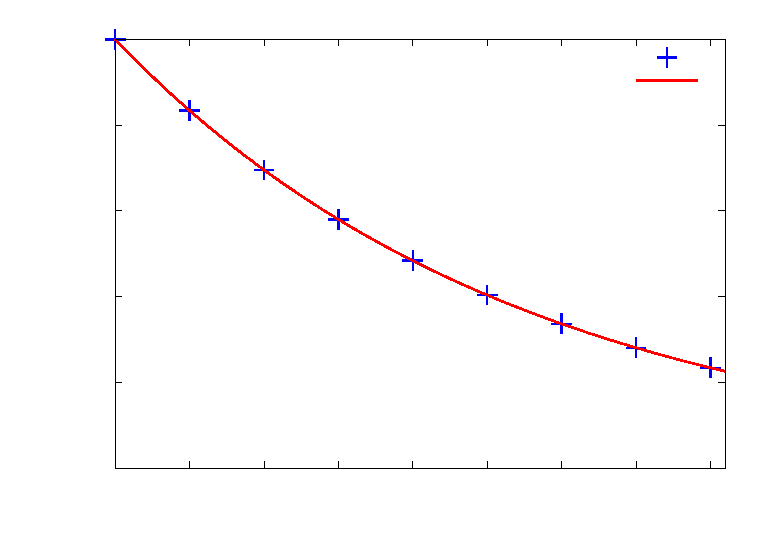
\includegraphics{plots/T1Erdmagnetfeld}}%
    \gplfronttext
  \end{picture}%
\endgroup

    \caption[$T_{1,e}$ measurement by varying $t$ and observing how the attenuation $\frac{\text{E}}{\text{E}_0}$ evolves.]{$T_{1,e}$ measurement by varying $t$ and observing how the attenuation $\frac{\text{E}}{\text{E}_0}$ evolves.
    The provided exponential fit results in a value for $T_{1,e}$ of \SI{2753.0500 \pm 0.0012}{\milli \second}.}
    \label{fig:T1Erdmagnetfeld}
\end{figure}
% !TEX root = main.tex
\section{Hahn echo}
\label{sec:Hahnecho}
The other relaxation measurement is the T$_2$ measurement. In order to understand that, we first have to explain the \textit{Hahn} echo and the principle of multiple echo sequences.\newline
The principle of the \textit{Hahn} echo is that an \SI{90}{\degree} pulse is applied and after a certain time $\tau$ a \SI{180}{\degree} pulse. The reason behind this method is that after the \SI{90}{\degree} pulse the spins are oriented in the transversal plane and start to precise around the earths magnetic field vector (z-axis). Due to spin-spin interaction (inhomogeneous magnetic field accrues) the spins also interact with each other and therefore some spins have a higher larmor frequency and some have a lower one. If an \SI{180}{\degree} pulse is applied after a certain time the spins will flip in the transversal plane and the slow precessing spins will be before the fast precessing spins again and when the fast precessing  overtake the slow ones again the B$_1$ coil will detect a signal again. The reason why the B$_1$ coil does not detect something while the slow and fast precessing spins are at different position is that they erase each other. If the spin-spin interaction is too weak than it also helps to de-shim the system along the x-direction. This also makes the homogeneous magnetic field inhomogeneous and thus the spins will get different larmor frequencies according to there position.\newline
Figure \ref{fig:Echobeispeilsignal} exemplary shows the \textit{Hahn} echo for a shimming value of \SI{4.95}{\milli \ampere} along the x-axis (original value \SI{10.11}{\milli \ampere}). It is also possible to change the time between the \SI{90}{\degree} and \SI{180}{\degree} pulse. This would shift the peak to higher times in the timescale and due to loss effects, the amplitude will shrink a little bit.
\begin{figure}[H]
    \centering
    % GNUPLOT: LaTeX picture with Postscript
\begingroup
  % Encoding inside the plot.  In the header of your document, this encoding
  % should to defined, e.g., by using
  % \usepackage[cp1252,<other encodings>]{inputenc}
  \inputencoding{cp1252}%
  \makeatletter
  \providecommand\color[2][]{%
    \GenericError{(gnuplot) \space\space\space\@spaces}{%
      Package color not loaded in conjunction with
      terminal option `colourtext'%
    }{See the gnuplot documentation for explanation.%
    }{Either use 'blacktext' in gnuplot or load the package
      color.sty in LaTeX.}%
    \renewcommand\color[2][]{}%
  }%
  \providecommand\includegraphics[2][]{%
    \GenericError{(gnuplot) \space\space\space\@spaces}{%
      Package graphicx or graphics not loaded%
    }{See the gnuplot documentation for explanation.%
    }{The gnuplot epslatex terminal needs graphicx.sty or graphics.sty.}%
    \renewcommand\includegraphics[2][]{}%
  }%
  \providecommand\rotatebox[2]{#2}%
  \@ifundefined{ifGPcolor}{%
    \newif\ifGPcolor
    \GPcolorfalse
  }{}%
  \@ifundefined{ifGPblacktext}{%
    \newif\ifGPblacktext
    \GPblacktexttrue
  }{}%
  % define a \g@addto@macro without @ in the name:
  \let\gplgaddtomacro\g@addto@macro
  % define empty templates for all commands taking text:
  \gdef\gplbacktext{}%
  \gdef\gplfronttext{}%
  \makeatother
  \ifGPblacktext
    % no textcolor at all
    \def\colorrgb#1{}%
    \def\colorgray#1{}%
  \else
    % gray or color?
    \ifGPcolor
      \def\colorrgb#1{\color[rgb]{#1}}%
      \def\colorgray#1{\color[gray]{#1}}%
      \expandafter\def\csname LTw\endcsname{\color{white}}%
      \expandafter\def\csname LTb\endcsname{\color{black}}%
      \expandafter\def\csname LTa\endcsname{\color{black}}%
      \expandafter\def\csname LT0\endcsname{\color[rgb]{1,0,0}}%
      \expandafter\def\csname LT1\endcsname{\color[rgb]{0,1,0}}%
      \expandafter\def\csname LT2\endcsname{\color[rgb]{0,0,1}}%
      \expandafter\def\csname LT3\endcsname{\color[rgb]{1,0,1}}%
      \expandafter\def\csname LT4\endcsname{\color[rgb]{0,1,1}}%
      \expandafter\def\csname LT5\endcsname{\color[rgb]{1,1,0}}%
      \expandafter\def\csname LT6\endcsname{\color[rgb]{0,0,0}}%
      \expandafter\def\csname LT7\endcsname{\color[rgb]{1,0.3,0}}%
      \expandafter\def\csname LT8\endcsname{\color[rgb]{0.5,0.5,0.5}}%
    \else
      % gray
      \def\colorrgb#1{\color{black}}%
      \def\colorgray#1{\color[gray]{#1}}%
      \expandafter\def\csname LTw\endcsname{\color{white}}%
      \expandafter\def\csname LTb\endcsname{\color{black}}%
      \expandafter\def\csname LTa\endcsname{\color{black}}%
      \expandafter\def\csname LT0\endcsname{\color{black}}%
      \expandafter\def\csname LT1\endcsname{\color{black}}%
      \expandafter\def\csname LT2\endcsname{\color{black}}%
      \expandafter\def\csname LT3\endcsname{\color{black}}%
      \expandafter\def\csname LT4\endcsname{\color{black}}%
      \expandafter\def\csname LT5\endcsname{\color{black}}%
      \expandafter\def\csname LT6\endcsname{\color{black}}%
      \expandafter\def\csname LT7\endcsname{\color{black}}%
      \expandafter\def\csname LT8\endcsname{\color{black}}%
    \fi
  \fi
    \setlength{\unitlength}{0.0500bp}%
    \ifx\gptboxheight\undefined%
      \newlength{\gptboxheight}%
      \newlength{\gptboxwidth}%
      \newsavebox{\gptboxtext}%
    \fi%
    \setlength{\fboxrule}{0.5pt}%
    \setlength{\fboxsep}{1pt}%
\begin{picture}(7200.00,5040.00)%
    \gplgaddtomacro\gplbacktext{%
      \csname LTb\endcsname%%
      \put(814,704){\makebox(0,0)[r]{\strut{}$-60$}}%
      \put(814,1390){\makebox(0,0)[r]{\strut{}$-40$}}%
      \put(814,2076){\makebox(0,0)[r]{\strut{}$-20$}}%
      \put(814,2762){\makebox(0,0)[r]{\strut{}$0$}}%
      \put(814,3447){\makebox(0,0)[r]{\strut{}$20$}}%
      \put(814,4133){\makebox(0,0)[r]{\strut{}$40$}}%
      \put(814,4819){\makebox(0,0)[r]{\strut{}$60$}}%
      \put(946,484){\makebox(0,0){\strut{}$0$}}%
      \put(1727,484){\makebox(0,0){\strut{}$0.2$}}%
      \put(2508,484){\makebox(0,0){\strut{}$0.4$}}%
      \put(3289,484){\makebox(0,0){\strut{}$0.6$}}%
      \put(4070,484){\makebox(0,0){\strut{}$0.8$}}%
      \put(4851,484){\makebox(0,0){\strut{}$1$}}%
      \put(5632,484){\makebox(0,0){\strut{}$1.2$}}%
      \put(6413,484){\makebox(0,0){\strut{}$1.4$}}%
    }%
    \gplgaddtomacro\gplfronttext{%
      \csname LTb\endcsname%%
      \put(209,2761){\rotatebox{-270}{\makebox(0,0){\strut{}Amplitude in $\si{\mu \volt}$}}}%
      \put(3874,154){\makebox(0,0){\strut{}Time in $\si{\second}$}}%
      \csname LTb\endcsname%%
      \put(5816,4646){\makebox(0,0)[r]{\strut{}shimming value: $\SI{4.95}{\milli \ampere}$ along x-axis}}%
    }%
    \gplbacktext
    \put(0,0){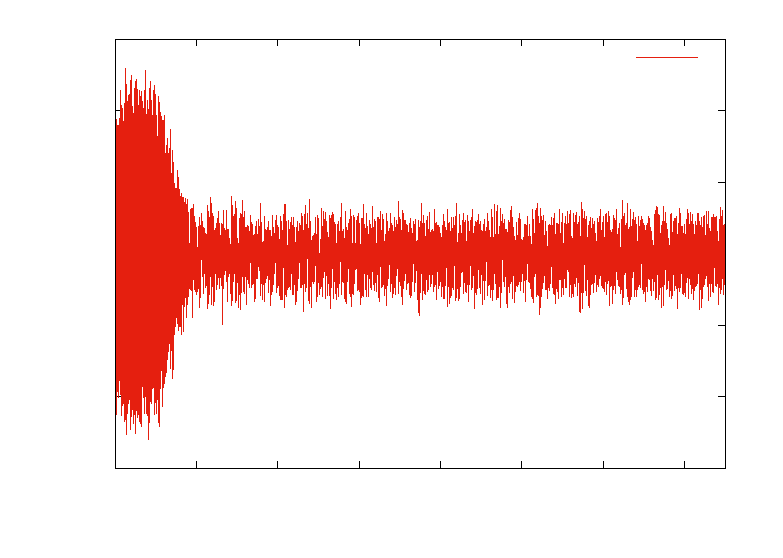
\includegraphics{plots/Echobeispeilsignal}}%
    \gplfronttext
  \end{picture}%
\endgroup

    \caption[Example of a single \textit{Hahn} echo for an echo time of \SI{0}{\milli \second}.]{Example of a single \textit{Hahn} echo for an echo time of \SI{0}{\milli \second}. The maximum of the echo is clearly visible. Due to relaxation after the maximum the signal after about \SI{0.2}{\second} is noise.}
    \label{fig:Echobeispeilsignal}
\end{figure}
It is also possible to fourier transform the signal from figure \ref{fig:Echobeispeilsignal}. Figure \ref{fig:SpinEcho} shows this for two different shimming values. The amplitude of the spectrum with the shimming value of \SI{0}{\milli \ampere} along the x-axis is clearly smaller than the amplitude of the spectrum with shimming value of \SI{4.95}{\milli \ampere} along the x-axis. This effect comes from the more inhomogeneous magnetic field of the spectrum with the shimming value of \SI{0}{\milli \ampere} along the x-axis. A more inhomogeneous magnetic field also means that the spins have more different larmor frequencies and thus the total intensity will shrink. The area under the spectrum should be independent from the inhomogeneity, because in total the magnetisation has to be the same. Only the distribution is different. This effect is also really good visible in the figure \ref{fig:SpinEcho}. This time it is not possible to find a good fitting function. Therefore this discussion is more qualitativ as mentioned before in chapter \ref{sec:OptimizationandCharacterisationofFIDinwatersample}. The reason why there is no good fitting function is that there are a lot of random peaks in the spectrum and the more peaks there are the more difficult it is to find a good fitting function. Another thing which makes it rather hard is that the frequency steps are not very small and thus there are not many datapoints to make a good fit. This was also a problem in chapter \ref{sec:OptimizationandCharacterisationofFIDinwatersample} as mentioned before.
\begin{figure}[H]
    \centering
    % GNUPLOT: LaTeX picture with Postscript
\begingroup
  % Encoding inside the plot.  In the header of your document, this encoding
  % should to defined, e.g., by using
  % \usepackage[cp1252,<other encodings>]{inputenc}
  \inputencoding{cp1252}%
  \makeatletter
  \providecommand\color[2][]{%
    \GenericError{(gnuplot) \space\space\space\@spaces}{%
      Package color not loaded in conjunction with
      terminal option `colourtext'%
    }{See the gnuplot documentation for explanation.%
    }{Either use 'blacktext' in gnuplot or load the package
      color.sty in LaTeX.}%
    \renewcommand\color[2][]{}%
  }%
  \providecommand\includegraphics[2][]{%
    \GenericError{(gnuplot) \space\space\space\@spaces}{%
      Package graphicx or graphics not loaded%
    }{See the gnuplot documentation for explanation.%
    }{The gnuplot epslatex terminal needs graphicx.sty or graphics.sty.}%
    \renewcommand\includegraphics[2][]{}%
  }%
  \providecommand\rotatebox[2]{#2}%
  \@ifundefined{ifGPcolor}{%
    \newif\ifGPcolor
    \GPcolorfalse
  }{}%
  \@ifundefined{ifGPblacktext}{%
    \newif\ifGPblacktext
    \GPblacktexttrue
  }{}%
  % define a \g@addto@macro without @ in the name:
  \let\gplgaddtomacro\g@addto@macro
  % define empty templates for all commands taking text:
  \gdef\gplbacktext{}%
  \gdef\gplfronttext{}%
  \makeatother
  \ifGPblacktext
    % no textcolor at all
    \def\colorrgb#1{}%
    \def\colorgray#1{}%
  \else
    % gray or color?
    \ifGPcolor
      \def\colorrgb#1{\color[rgb]{#1}}%
      \def\colorgray#1{\color[gray]{#1}}%
      \expandafter\def\csname LTw\endcsname{\color{white}}%
      \expandafter\def\csname LTb\endcsname{\color{black}}%
      \expandafter\def\csname LTa\endcsname{\color{black}}%
      \expandafter\def\csname LT0\endcsname{\color[rgb]{1,0,0}}%
      \expandafter\def\csname LT1\endcsname{\color[rgb]{0,1,0}}%
      \expandafter\def\csname LT2\endcsname{\color[rgb]{0,0,1}}%
      \expandafter\def\csname LT3\endcsname{\color[rgb]{1,0,1}}%
      \expandafter\def\csname LT4\endcsname{\color[rgb]{0,1,1}}%
      \expandafter\def\csname LT5\endcsname{\color[rgb]{1,1,0}}%
      \expandafter\def\csname LT6\endcsname{\color[rgb]{0,0,0}}%
      \expandafter\def\csname LT7\endcsname{\color[rgb]{1,0.3,0}}%
      \expandafter\def\csname LT8\endcsname{\color[rgb]{0.5,0.5,0.5}}%
    \else
      % gray
      \def\colorrgb#1{\color{black}}%
      \def\colorgray#1{\color[gray]{#1}}%
      \expandafter\def\csname LTw\endcsname{\color{white}}%
      \expandafter\def\csname LTb\endcsname{\color{black}}%
      \expandafter\def\csname LTa\endcsname{\color{black}}%
      \expandafter\def\csname LT0\endcsname{\color{black}}%
      \expandafter\def\csname LT1\endcsname{\color{black}}%
      \expandafter\def\csname LT2\endcsname{\color{black}}%
      \expandafter\def\csname LT3\endcsname{\color{black}}%
      \expandafter\def\csname LT4\endcsname{\color{black}}%
      \expandafter\def\csname LT5\endcsname{\color{black}}%
      \expandafter\def\csname LT6\endcsname{\color{black}}%
      \expandafter\def\csname LT7\endcsname{\color{black}}%
      \expandafter\def\csname LT8\endcsname{\color{black}}%
    \fi
  \fi
    \setlength{\unitlength}{0.0500bp}%
    \ifx\gptboxheight\undefined%
      \newlength{\gptboxheight}%
      \newlength{\gptboxwidth}%
      \newsavebox{\gptboxtext}%
    \fi%
    \setlength{\fboxrule}{0.5pt}%
    \setlength{\fboxsep}{1pt}%
\begin{picture}(7200.00,5040.00)%
    \gplgaddtomacro\gplbacktext{%
      \csname LTb\endcsname%%
      \put(682,704){\makebox(0,0)[r]{\strut{}$0$}}%
      \put(682,1253){\makebox(0,0)[r]{\strut{}$2$}}%
      \put(682,1801){\makebox(0,0)[r]{\strut{}$4$}}%
      \put(682,2350){\makebox(0,0)[r]{\strut{}$6$}}%
      \put(682,2899){\makebox(0,0)[r]{\strut{}$8$}}%
      \put(682,3447){\makebox(0,0)[r]{\strut{}$10$}}%
      \put(682,3996){\makebox(0,0)[r]{\strut{}$12$}}%
      \put(682,4545){\makebox(0,0)[r]{\strut{}$14$}}%
      \put(814,484){\makebox(0,0){\strut{}$1800$}}%
      \put(1563,484){\makebox(0,0){\strut{}$1810$}}%
      \put(2311,484){\makebox(0,0){\strut{}$1820$}}%
      \put(3060,484){\makebox(0,0){\strut{}$1830$}}%
      \put(3809,484){\makebox(0,0){\strut{}$1840$}}%
      \put(4557,484){\makebox(0,0){\strut{}$1850$}}%
      \put(5306,484){\makebox(0,0){\strut{}$1860$}}%
      \put(6054,484){\makebox(0,0){\strut{}$1870$}}%
      \put(6803,484){\makebox(0,0){\strut{}$1880$}}%
    }%
    \gplgaddtomacro\gplfronttext{%
      \csname LTb\endcsname%%
      \put(209,2761){\rotatebox{-270}{\makebox(0,0){\strut{}FID amplitude}}}%
      \put(3808,154){\makebox(0,0){\strut{}Frequency in $\si{}{Hz}$}}%
      \csname LTb\endcsname%%
      \put(5816,4646){\makebox(0,0)[r]{\strut{}shimmin value $x = \si{0}{}}}%
      \csname LTb\endcsname%%
      \put(5816,4426){\makebox(0,0)[r]{\strut{}shimmin value $x = \si{4.95}{}}}%
    }%
    \gplbacktext
    \put(0,0){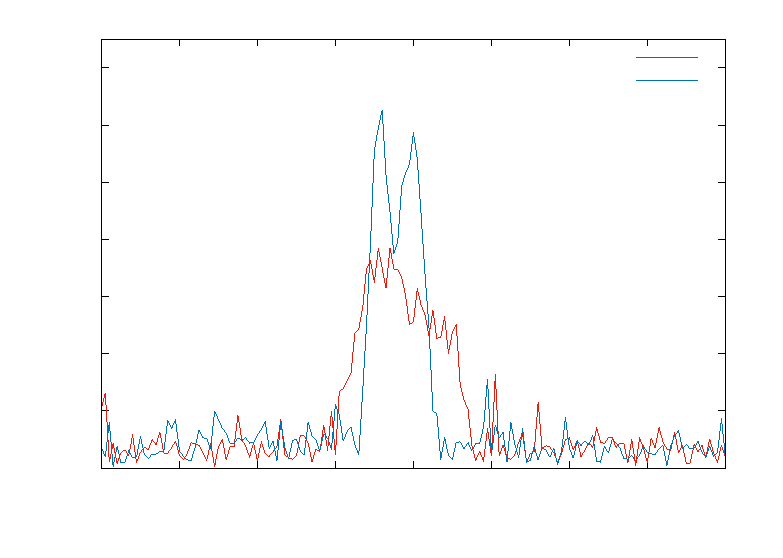
\includegraphics{plots/SpinEcho_4scans_ideal_Repetitiontime_0_shimming_150echo}}%
    \gplfronttext
  \end{picture}%
\endgroup

    \caption[Spectrum of a single \textit{Hahn} echo applied by different shimming values.]{Spectrum of a single \textit{Hahn} echo applied by different shimming values. Due to more de-shimming of the red curve, the apmlitude is lower. Nevertheless the area under the spectrum is the same, due to the same magnetisation.}
    \label{fig:SpinEcho}
\end{figure}
For the following chapter it is specifcally important to know which relaxation time we observe. Due to the inhomogeneous magnetic field there exist different relaxation times of the transversal relaxation time T$_2$. The transversal relaxation time T$_2^*$ describes the relaxation in consideration of the inhomogeneous magentic field. Therefore the formula has following shape:
\begin{align}
    \frac{1}{T_2^*} = \frac{1}{T_2} + \gamma \Delta B_0 \ .
    \label{eq:T2_star}
\end{align}
In this equation $\gamma$ is the gyromagnetic ratio of the probe and $\Delta B_0$ is the difference of the magnetic field to its equilibrium. Knowing that we now know that every time we de-shim the system we observe T$_2^*$ and not T$_2$.

% !TEX root = main.tex
\section{Multiple echo sequences}
\label{sec:Multipleechosequences}
Beside the \textit{Hahn} echo it is also possible to apply multiple \textit{Hahn} echos in one experimental measurement. This method is called \textit{Call-Purcell-Meiboom-Gill}-method (CPMG). Therefore the \SI{180}{\degree} pulse is applied every $2\tau$ and thus there accur many maximums in the signal every $2\tau$. The reason to use the CPMG method is that it is possible to measure the amplitude of two consecutiv maxima more often and therefore the measurement of T$_2$ is more precise. More about this will be discussed in the next chapter.\newline
To make the CPMG signals smoother in the time domain we do not use rectangular functions for the pulses, but smoothen them at the edge by a \textit{sine-bell-square} function. This is possible, due to the fact that it does not change the physical properties of our measurements, but will make them smoother.\newline
A main advantage of CMPG is that errors in the refocusing pulse can be vanished (minimize term of inhomogeneous magnetic field), by changing the phase between the B$_1$ excitation and the refocusing pulses. The program \textit{Prospa} profides a function called ''Constant 180 pulse phase''. This function keeps all the phases of the refocusing pulses equal. The second function \textit{Prospa} provides is ''Alternating 180 pulse phase''. This function compensates echo errors by alternating the refocusing pulses by \SI{180}{\degree}. In figure \ref{fig:180pulsephasedegree} it is visible what a change in the 180 pulse phase does to the signal. Unfortunately we only saved the signal vor 180 pulse phases of \SI{270}{\degree} and \SI{90}{\degree}. For those two values the signal does not change. That is also the reason why there is only one signal visible. The other one is just directly behind the other one and therefore not visible. If we would have saved a pulse phase of \SI{0}{\degree} or \SI{180}{\degree} the signal should change to a way faster decay and so the amplitude dies away really quickly.

\begin{figure}[H]
    \centering
    % GNUPLOT: LaTeX picture with Postscript
\begingroup
  % Encoding inside the plot.  In the header of your document, this encoding
  % should to defined, e.g., by using
  % \usepackage[cp1252,<other encodings>]{inputenc}
  \inputencoding{cp1252}%
  \makeatletter
  \providecommand\color[2][]{%
    \GenericError{(gnuplot) \space\space\space\@spaces}{%
      Package color not loaded in conjunction with
      terminal option `colourtext'%
    }{See the gnuplot documentation for explanation.%
    }{Either use 'blacktext' in gnuplot or load the package
      color.sty in LaTeX.}%
    \renewcommand\color[2][]{}%
  }%
  \providecommand\includegraphics[2][]{%
    \GenericError{(gnuplot) \space\space\space\@spaces}{%
      Package graphicx or graphics not loaded%
    }{See the gnuplot documentation for explanation.%
    }{The gnuplot epslatex terminal needs graphicx.sty or graphics.sty.}%
    \renewcommand\includegraphics[2][]{}%
  }%
  \providecommand\rotatebox[2]{#2}%
  \@ifundefined{ifGPcolor}{%
    \newif\ifGPcolor
    \GPcolorfalse
  }{}%
  \@ifundefined{ifGPblacktext}{%
    \newif\ifGPblacktext
    \GPblacktexttrue
  }{}%
  % define a \g@addto@macro without @ in the name:
  \let\gplgaddtomacro\g@addto@macro
  % define empty templates for all commands taking text:
  \gdef\gplbacktext{}%
  \gdef\gplfronttext{}%
  \makeatother
  \ifGPblacktext
    % no textcolor at all
    \def\colorrgb#1{}%
    \def\colorgray#1{}%
  \else
    % gray or color?
    \ifGPcolor
      \def\colorrgb#1{\color[rgb]{#1}}%
      \def\colorgray#1{\color[gray]{#1}}%
      \expandafter\def\csname LTw\endcsname{\color{white}}%
      \expandafter\def\csname LTb\endcsname{\color{black}}%
      \expandafter\def\csname LTa\endcsname{\color{black}}%
      \expandafter\def\csname LT0\endcsname{\color[rgb]{1,0,0}}%
      \expandafter\def\csname LT1\endcsname{\color[rgb]{0,1,0}}%
      \expandafter\def\csname LT2\endcsname{\color[rgb]{0,0,1}}%
      \expandafter\def\csname LT3\endcsname{\color[rgb]{1,0,1}}%
      \expandafter\def\csname LT4\endcsname{\color[rgb]{0,1,1}}%
      \expandafter\def\csname LT5\endcsname{\color[rgb]{1,1,0}}%
      \expandafter\def\csname LT6\endcsname{\color[rgb]{0,0,0}}%
      \expandafter\def\csname LT7\endcsname{\color[rgb]{1,0.3,0}}%
      \expandafter\def\csname LT8\endcsname{\color[rgb]{0.5,0.5,0.5}}%
    \else
      % gray
      \def\colorrgb#1{\color{black}}%
      \def\colorgray#1{\color[gray]{#1}}%
      \expandafter\def\csname LTw\endcsname{\color{white}}%
      \expandafter\def\csname LTb\endcsname{\color{black}}%
      \expandafter\def\csname LTa\endcsname{\color{black}}%
      \expandafter\def\csname LT0\endcsname{\color{black}}%
      \expandafter\def\csname LT1\endcsname{\color{black}}%
      \expandafter\def\csname LT2\endcsname{\color{black}}%
      \expandafter\def\csname LT3\endcsname{\color{black}}%
      \expandafter\def\csname LT4\endcsname{\color{black}}%
      \expandafter\def\csname LT5\endcsname{\color{black}}%
      \expandafter\def\csname LT6\endcsname{\color{black}}%
      \expandafter\def\csname LT7\endcsname{\color{black}}%
      \expandafter\def\csname LT8\endcsname{\color{black}}%
    \fi
  \fi
    \setlength{\unitlength}{0.0500bp}%
    \ifx\gptboxheight\undefined%
      \newlength{\gptboxheight}%
      \newlength{\gptboxwidth}%
      \newsavebox{\gptboxtext}%
    \fi%
    \setlength{\fboxrule}{0.5pt}%
    \setlength{\fboxsep}{1pt}%
\begin{picture}(7200.00,5040.00)%
    \gplgaddtomacro\gplbacktext{%
      \csname LTb\endcsname%%
      \put(814,704){\makebox(0,0)[r]{\strut{}$-60$}}%
      \put(814,1390){\makebox(0,0)[r]{\strut{}$-40$}}%
      \put(814,2076){\makebox(0,0)[r]{\strut{}$-20$}}%
      \put(814,2762){\makebox(0,0)[r]{\strut{}$0$}}%
      \put(814,3447){\makebox(0,0)[r]{\strut{}$20$}}%
      \put(814,4133){\makebox(0,0)[r]{\strut{}$40$}}%
      \put(814,4819){\makebox(0,0)[r]{\strut{}$60$}}%
      \put(946,484){\makebox(0,0){\strut{}$0$}}%
      \put(1783,484){\makebox(0,0){\strut{}$1000$}}%
      \put(2619,484){\makebox(0,0){\strut{}$2000$}}%
      \put(3456,484){\makebox(0,0){\strut{}$3000$}}%
      \put(4293,484){\makebox(0,0){\strut{}$4000$}}%
      \put(5130,484){\makebox(0,0){\strut{}$5000$}}%
      \put(5966,484){\makebox(0,0){\strut{}$6000$}}%
      \put(6803,484){\makebox(0,0){\strut{}$7000$}}%
    }%
    \gplgaddtomacro\gplfronttext{%
      \csname LTb\endcsname%%
      \put(209,2761){\rotatebox{-270}{\makebox(0,0){\strut{}Amplitude in $\si{\mu \volt}$}}}%
      \put(3874,154){\makebox(0,0){\strut{}Time in $\si{\second}$}}%
      \csname LTb\endcsname%%
      \put(5816,4646){\makebox(0,0)[r]{\strut{}180 pulse phase \SI{270}{\degree}}}%
      \csname LTb\endcsname%%
      \put(5816,4426){\makebox(0,0)[r]{\strut{}180 pulse phase \SI{90}{\degree}}}%
    }%
    \gplbacktext
    \put(0,0){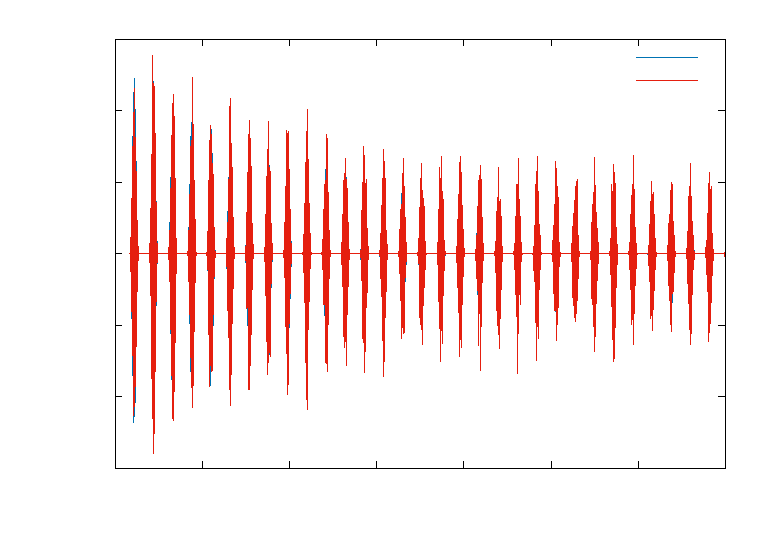
\includegraphics{plots/180pulsephasedegree}}%
    \gplfronttext
  \end{picture}%
\endgroup

    \caption[This figure shows the impact of the 180 pulse phase.]{This figure shows the impact of the 180 pulse phase. Unfortunately we only saved data for a 180 pulse phase of \SI{270}{\degree} and \SI{90}{\degree} and for those values it is correct that the signal does not change, but a signal for a 180 pulse phase of \SI{180}{\degree} would have shown a different signal.}
    \label{fig:180pulsephasedegree}
\end{figure}
 
% !TEX root = main.tex
\section{Transversal relaxation measurements}
\label{sec:Transversalrelaxationmeasurements}
The last chapter in the first part of this experiment is the transversal relaxation measurement. In order to do so there are two possible ways again.\newline
The first one is by one single \textit{Hahn} echo (spin echo). Therefore the ratio between the maximum of the signal after the \SI{90}{\degree} pulse and the maximum after the echo (maximum after $2\tau$) provides the transversal relaxation time T$_2$. Figure \ref{fig:T2} shows measurements for this method by different echo time steps of $2\cdot \SI{400}{\milli \second}$. The exponential decay is clearly visible, due to the already explained loss of phase coherence between the spins. Therefore to fit the datapoints the following formula has been used:
\begin{align}
    M(x)=M_0 \cdot exp\left(\frac{-x}{T_{2}}\right) \ .
 \label{eq:T2}
\end{align}
This formula shows a T$_2$ relaxation time of \SI{2691 \pm 12}{\milli \second}. Remember that the phase coherence loss because of the spin spin relaxation is irreversible and is always obtained when measuring T$_2$.

\begin{figure}[H]
    \centering
    % GNUPLOT: LaTeX picture with Postscript
\begingroup
  % Encoding inside the plot.  In the header of your document, this encoding
  % should to defined, e.g., by using
  % \usepackage[cp1252,<other encodings>]{inputenc}
  \inputencoding{cp1252}%
  \makeatletter
  \providecommand\color[2][]{%
    \GenericError{(gnuplot) \space\space\space\@spaces}{%
      Package color not loaded in conjunction with
      terminal option `colourtext'%
    }{See the gnuplot documentation for explanation.%
    }{Either use 'blacktext' in gnuplot or load the package
      color.sty in LaTeX.}%
    \renewcommand\color[2][]{}%
  }%
  \providecommand\includegraphics[2][]{%
    \GenericError{(gnuplot) \space\space\space\@spaces}{%
      Package graphicx or graphics not loaded%
    }{See the gnuplot documentation for explanation.%
    }{The gnuplot epslatex terminal needs graphicx.sty or graphics.sty.}%
    \renewcommand\includegraphics[2][]{}%
  }%
  \providecommand\rotatebox[2]{#2}%
  \@ifundefined{ifGPcolor}{%
    \newif\ifGPcolor
    \GPcolorfalse
  }{}%
  \@ifundefined{ifGPblacktext}{%
    \newif\ifGPblacktext
    \GPblacktexttrue
  }{}%
  % define a \g@addto@macro without @ in the name:
  \let\gplgaddtomacro\g@addto@macro
  % define empty templates for all commands taking text:
  \gdef\gplbacktext{}%
  \gdef\gplfronttext{}%
  \makeatother
  \ifGPblacktext
    % no textcolor at all
    \def\colorrgb#1{}%
    \def\colorgray#1{}%
  \else
    % gray or color?
    \ifGPcolor
      \def\colorrgb#1{\color[rgb]{#1}}%
      \def\colorgray#1{\color[gray]{#1}}%
      \expandafter\def\csname LTw\endcsname{\color{white}}%
      \expandafter\def\csname LTb\endcsname{\color{black}}%
      \expandafter\def\csname LTa\endcsname{\color{black}}%
      \expandafter\def\csname LT0\endcsname{\color[rgb]{1,0,0}}%
      \expandafter\def\csname LT1\endcsname{\color[rgb]{0,1,0}}%
      \expandafter\def\csname LT2\endcsname{\color[rgb]{0,0,1}}%
      \expandafter\def\csname LT3\endcsname{\color[rgb]{1,0,1}}%
      \expandafter\def\csname LT4\endcsname{\color[rgb]{0,1,1}}%
      \expandafter\def\csname LT5\endcsname{\color[rgb]{1,1,0}}%
      \expandafter\def\csname LT6\endcsname{\color[rgb]{0,0,0}}%
      \expandafter\def\csname LT7\endcsname{\color[rgb]{1,0.3,0}}%
      \expandafter\def\csname LT8\endcsname{\color[rgb]{0.5,0.5,0.5}}%
    \else
      % gray
      \def\colorrgb#1{\color{black}}%
      \def\colorgray#1{\color[gray]{#1}}%
      \expandafter\def\csname LTw\endcsname{\color{white}}%
      \expandafter\def\csname LTb\endcsname{\color{black}}%
      \expandafter\def\csname LTa\endcsname{\color{black}}%
      \expandafter\def\csname LT0\endcsname{\color{black}}%
      \expandafter\def\csname LT1\endcsname{\color{black}}%
      \expandafter\def\csname LT2\endcsname{\color{black}}%
      \expandafter\def\csname LT3\endcsname{\color{black}}%
      \expandafter\def\csname LT4\endcsname{\color{black}}%
      \expandafter\def\csname LT5\endcsname{\color{black}}%
      \expandafter\def\csname LT6\endcsname{\color{black}}%
      \expandafter\def\csname LT7\endcsname{\color{black}}%
      \expandafter\def\csname LT8\endcsname{\color{black}}%
    \fi
  \fi
    \setlength{\unitlength}{0.0500bp}%
    \ifx\gptboxheight\undefined%
      \newlength{\gptboxheight}%
      \newlength{\gptboxwidth}%
      \newsavebox{\gptboxtext}%
    \fi%
    \setlength{\fboxrule}{0.5pt}%
    \setlength{\fboxsep}{1pt}%
\begin{picture}(7200.00,5040.00)%
    \gplgaddtomacro\gplbacktext{%
      \csname LTb\endcsname%%
      \put(814,704){\makebox(0,0)[r]{\strut{}$0$}}%
      \put(814,1527){\makebox(0,0)[r]{\strut{}$0.2$}}%
      \put(814,2350){\makebox(0,0)[r]{\strut{}$0.4$}}%
      \put(814,3173){\makebox(0,0)[r]{\strut{}$0.6$}}%
      \put(814,3996){\makebox(0,0)[r]{\strut{}$0.8$}}%
      \put(814,4819){\makebox(0,0)[r]{\strut{}$1$}}%
      \put(946,484){\makebox(0,0){\strut{}$0$}}%
      \put(1727,484){\makebox(0,0){\strut{}$1000$}}%
      \put(2508,484){\makebox(0,0){\strut{}$2000$}}%
      \put(3289,484){\makebox(0,0){\strut{}$3000$}}%
      \put(4070,484){\makebox(0,0){\strut{}$4000$}}%
      \put(4851,484){\makebox(0,0){\strut{}$5000$}}%
      \put(5632,484){\makebox(0,0){\strut{}$6000$}}%
      \put(6413,484){\makebox(0,0){\strut{}$7000$}}%
    }%
    \gplgaddtomacro\gplfronttext{%
      \csname LTb\endcsname%%
      \put(209,2761){\rotatebox{-270}{\makebox(0,0){\strut{}Attenuation $\frac{\text{E}}{\text{E}_0}$}}}%
      \put(3874,154){\makebox(0,0){\strut{}Time in $\si{\milli \second}$}}%
      \csname LTb\endcsname%%
      \put(5816,4646){\makebox(0,0)[r]{\strut{}measured data}}%
      \csname LTb\endcsname%%
      \put(5816,4426){\makebox(0,0)[r]{\strut{}attenuation Fit}}%
    }%
    \gplbacktext
    \put(0,0){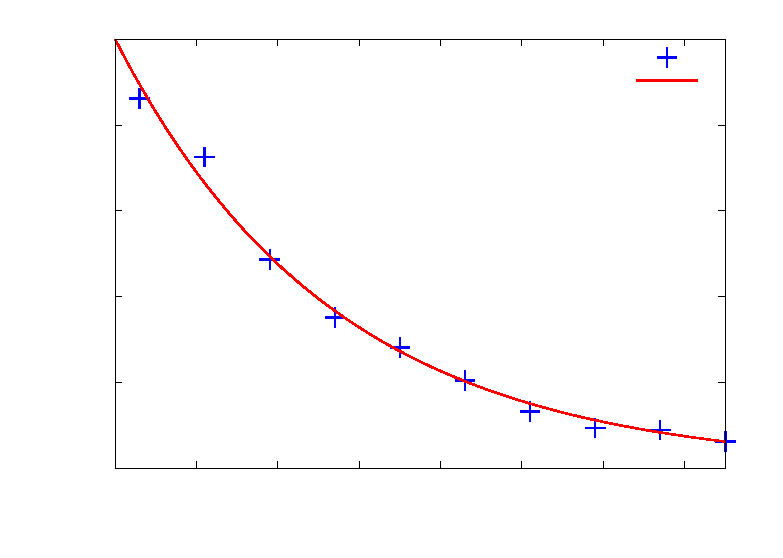
\includegraphics{plots/T2}}%
    \gplfronttext
  \end{picture}%
\endgroup

    \caption[Attenuation $\frac{\text{E}}{\text{E}_0}$ for different echo times and exponential fit.]{Attenuation $\frac{\text{E}}{\text{E}_0}$ for different echo times and exponential fit. The applied exponential fit results in a value for T$_2$ of \SI{2691 \pm 12}{\milli \second}.}
    \label{fig:T2}
\end{figure}

One disadvantage of the T$_2$ measurement via one single \textit{Hahn} echo is that the ratio of two back to back maxima is not that exact. Therefore the second option to measure T$_2$ is by using CPMG. Now that more maximums can be observed, the ratio of back to back maxima can be calculated more precisely. Therefore the result of T$_2$ is more exact using this method. Figure \ref{fig:CPMG} shows measured data for 30 different echos. Due to the exponential decay the formula \eqref{eq:T2} has been used again to fit the measured data. This results in a value for T$_2$ of \SI{2317.76000 \pm 0.00062}{\milli \second}. It is clearly visible that the uncertainty of this value is way below the value of the measurement via one single \textit{Hahn} echo, therefore it is more exact. A comparison with an example literature value of \SI{2000}{\milli \second} \cite{literaturT1} shows that the magnitude is correct. Keep in mind that a comparison to literature values is just there to get the magnitude. Since the surrounding magnetic field and the probe define the exact value as mentioned before.

\begin{figure}[H]
    \centering
    % GNUPLOT: LaTeX picture with Postscript
\begingroup
  % Encoding inside the plot.  In the header of your document, this encoding
  % should to defined, e.g., by using
  % \usepackage[cp1252,<other encodings>]{inputenc}
  \inputencoding{cp1252}%
  \makeatletter
  \providecommand\color[2][]{%
    \GenericError{(gnuplot) \space\space\space\@spaces}{%
      Package color not loaded in conjunction with
      terminal option `colourtext'%
    }{See the gnuplot documentation for explanation.%
    }{Either use 'blacktext' in gnuplot or load the package
      color.sty in LaTeX.}%
    \renewcommand\color[2][]{}%
  }%
  \providecommand\includegraphics[2][]{%
    \GenericError{(gnuplot) \space\space\space\@spaces}{%
      Package graphicx or graphics not loaded%
    }{See the gnuplot documentation for explanation.%
    }{The gnuplot epslatex terminal needs graphicx.sty or graphics.sty.}%
    \renewcommand\includegraphics[2][]{}%
  }%
  \providecommand\rotatebox[2]{#2}%
  \@ifundefined{ifGPcolor}{%
    \newif\ifGPcolor
    \GPcolorfalse
  }{}%
  \@ifundefined{ifGPblacktext}{%
    \newif\ifGPblacktext
    \GPblacktexttrue
  }{}%
  % define a \g@addto@macro without @ in the name:
  \let\gplgaddtomacro\g@addto@macro
  % define empty templates for all commands taking text:
  \gdef\gplbacktext{}%
  \gdef\gplfronttext{}%
  \makeatother
  \ifGPblacktext
    % no textcolor at all
    \def\colorrgb#1{}%
    \def\colorgray#1{}%
  \else
    % gray or color?
    \ifGPcolor
      \def\colorrgb#1{\color[rgb]{#1}}%
      \def\colorgray#1{\color[gray]{#1}}%
      \expandafter\def\csname LTw\endcsname{\color{white}}%
      \expandafter\def\csname LTb\endcsname{\color{black}}%
      \expandafter\def\csname LTa\endcsname{\color{black}}%
      \expandafter\def\csname LT0\endcsname{\color[rgb]{1,0,0}}%
      \expandafter\def\csname LT1\endcsname{\color[rgb]{0,1,0}}%
      \expandafter\def\csname LT2\endcsname{\color[rgb]{0,0,1}}%
      \expandafter\def\csname LT3\endcsname{\color[rgb]{1,0,1}}%
      \expandafter\def\csname LT4\endcsname{\color[rgb]{0,1,1}}%
      \expandafter\def\csname LT5\endcsname{\color[rgb]{1,1,0}}%
      \expandafter\def\csname LT6\endcsname{\color[rgb]{0,0,0}}%
      \expandafter\def\csname LT7\endcsname{\color[rgb]{1,0.3,0}}%
      \expandafter\def\csname LT8\endcsname{\color[rgb]{0.5,0.5,0.5}}%
    \else
      % gray
      \def\colorrgb#1{\color{black}}%
      \def\colorgray#1{\color[gray]{#1}}%
      \expandafter\def\csname LTw\endcsname{\color{white}}%
      \expandafter\def\csname LTb\endcsname{\color{black}}%
      \expandafter\def\csname LTa\endcsname{\color{black}}%
      \expandafter\def\csname LT0\endcsname{\color{black}}%
      \expandafter\def\csname LT1\endcsname{\color{black}}%
      \expandafter\def\csname LT2\endcsname{\color{black}}%
      \expandafter\def\csname LT3\endcsname{\color{black}}%
      \expandafter\def\csname LT4\endcsname{\color{black}}%
      \expandafter\def\csname LT5\endcsname{\color{black}}%
      \expandafter\def\csname LT6\endcsname{\color{black}}%
      \expandafter\def\csname LT7\endcsname{\color{black}}%
      \expandafter\def\csname LT8\endcsname{\color{black}}%
    \fi
  \fi
    \setlength{\unitlength}{0.0500bp}%
    \ifx\gptboxheight\undefined%
      \newlength{\gptboxheight}%
      \newlength{\gptboxwidth}%
      \newsavebox{\gptboxtext}%
    \fi%
    \setlength{\fboxrule}{0.5pt}%
    \setlength{\fboxsep}{1pt}%
\begin{picture}(7200.00,5040.00)%
    \gplgaddtomacro\gplbacktext{%
      \csname LTb\endcsname%%
      \put(814,704){\makebox(0,0)[r]{\strut{}$0$}}%
      \put(814,1527){\makebox(0,0)[r]{\strut{}$0.2$}}%
      \put(814,2350){\makebox(0,0)[r]{\strut{}$0.4$}}%
      \put(814,3173){\makebox(0,0)[r]{\strut{}$0.6$}}%
      \put(814,3996){\makebox(0,0)[r]{\strut{}$0.8$}}%
      \put(814,4819){\makebox(0,0)[r]{\strut{}$1$}}%
      \put(1754,484){\makebox(0,0){\strut{}$1000$}}%
      \put(2764,484){\makebox(0,0){\strut{}$2000$}}%
      \put(3774,484){\makebox(0,0){\strut{}$3000$}}%
      \put(4783,484){\makebox(0,0){\strut{}$4000$}}%
      \put(5793,484){\makebox(0,0){\strut{}$5000$}}%
      \put(6803,484){\makebox(0,0){\strut{}$6000$}}%
    }%
    \gplgaddtomacro\gplfronttext{%
      \csname LTb\endcsname%%
      \put(209,2761){\rotatebox{-270}{\makebox(0,0){\strut{}Amplitude $\frac{\text{E}}{\text{E}_0}$}}}%
      \put(3874,154){\makebox(0,0){\strut{}Time in $\si{\milli \second}$}}%
      \csname LTb\endcsname%%
      \put(5816,4646){\makebox(0,0)[r]{\strut{}measured data}}%
      \csname LTb\endcsname%%
      \put(5816,4426){\makebox(0,0)[r]{\strut{}attenuation-Fit}}%
    }%
    \gplbacktext
    \put(0,0){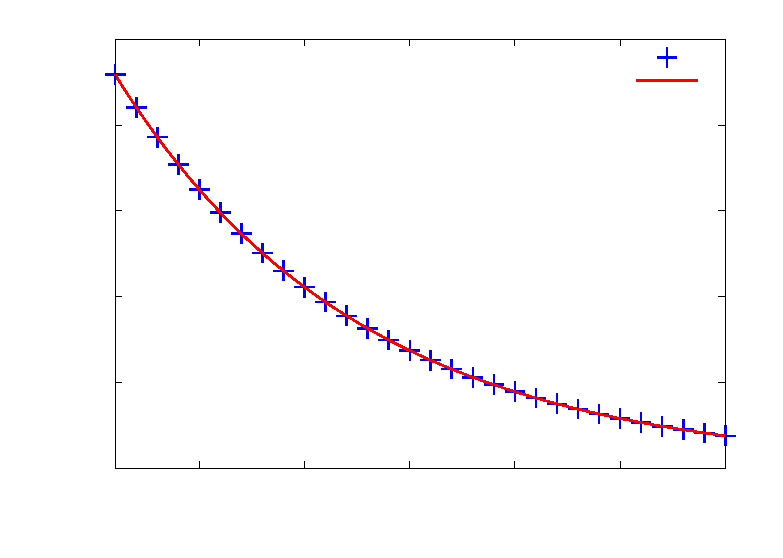
\includegraphics{plots/CPMG045shimming}}%
    \gplfronttext
  \end{picture}%
\endgroup

    \caption[Attenuation $\frac{\text{E}}{\text{E}_0}$ for different echo maxima provided by the CPMG method.]{Attenuation $\frac{\text{E}}{\text{E}_0}$ for different echo maxima provided by the CPMG method. The applied exponential fit results in a value for T$_2$ of \SI{2317.76000 \pm 0.00062}{\milli \second}.}
    \label{fig:CPMG}
\end{figure}

The difference of the two T$_2$ values might occur, due to deshimming the system for the CPMG method and therefore can always be some inaccurate pulse phases. Nevertheless note that the CPMG method is the more exact method to measure T$_2$, due to more back to back maxima. By measuring T$_2$ via the \textit{Hahn} echo and the CPMG the inhomogeneity of the magnetic field is reversed in theory, due to the \SI{180}{\degree} pulses and therefore should not have a big impact on the relaxation time. Nevertheless due to inaccurate pulse phases, deshimming can still have a small impact. That is probably why the two relxation times are not the same.
\selectlanguage{ngerman}
\newpage
\textcolor{red}{@Philipp ab hier Alle TITEL, BUs, LEGENDEN nochmal korrigieren!! ''todo''}
% !TEX root = main.tex
\subsection{\textcolor{red}{ToDo!}Relaxationskontrast}
\label{sec:Signalintensitaet}
Da der zweite Teil des Experiments an einem anderen Versuchstag durchgeführt wurde, wurde zu Beginn erneut eine Optimierung des Aufbaus auf die Wasserprobe vorgenommen um die Vergleichbarkeit der Ergebnisse der beiden Versuchstage zu schaffen. Dies geschah analog zum Vorgehen, welches in Abschnitt \ref{sec:OptimizationandCharacterisationofFIDinwatersample} dargelegt wurde.

Der Versuchsteil selbst zielt darauf ab zu untersuchen, wie longitudinale ($T_1$) und transversale ($T_2$) Relaxationszeit durch paramagnetische Ionen beeinflusst werden können. 
Weiterführend kann dadurch -- abhängig von $T_1$ und $T_2$ -- der Kontrast innerhalb eines bildgebenden Verfahrens verändert werden und somit können verschiedene Bereiche einer Probe besser aufgelöst und analysiert werden. 
Daher sollen die sogenannte Relaxivitäten $r_1$ und $r_2$ nach
\begin{align}
    \frac{1}{T_{\text{i}}\left([\ce{X^2+}]\right)} = r_{\text{i}} \cdot [\ce{X^2+}] + \frac{1}{T_{\text{i}}(0)} \label{eq:relaxivitat}
\end{align}
bestimmt werden. Dabei bezeichnet $T_{\text{i}}\left([\ce{X^2+}]\right)$ die -- von der Konzentration des verwendeten paramagnetischen Salzes im Wasser abhängige -- jeweilige Relaxationszeit, $[\ce{X^2+}]$  die entsprechende Ionenkonzentration und $T_{\text{i}}(0)$ die Relaxtionszeit im Falle, dass kein Kontrastmittel verwendet wird.




\begin{figure}[H]
    \centering
    % !TEX root = main.tex
\section{Fourietrafo der Messungen mit unterschieldicheer Polarisationszeit}
\begin{figure}[H]
    \centering
    % !TEX root = main.tex
\section{Fourietrafo der Messungen mit unterschieldicheer Polarisationszeit}
\begin{figure}[H]
    \centering
    \input{plots/Polarisationszeit.tex}
    \caption{Amplitude in abhängigkeit von zwei verschiedenen Piolarisatiosnzeiten}
\end{figure}
    \caption{Amplitude in abhängigkeit von zwei verschiedenen Piolarisatiosnzeiten}
\end{figure}
    \caption[Abhängigkeit der Signalintensität von der Polarisationszeit.]{In dieser Abbildung sind zwei ,,Pulse and Collect''-Messungen der bidestillierten Wasserprobe dargestellt. Die rote Kurve zeigt eine Messung mit einer Polarisationszeit von $\SI{4}{\second}$, bei der blauen Kurve beträgt die Polarisationszeit $\SI{0.5}{\second}$. Hierbei ist deutlich zu erkennen, dass die Signalintensität durch die höhere Polarisationszeit deutlich gesteigert werden kann. Bei den dargestellten Messungen um circa Faktor drei.} 
    \label{fig:SignalintensitaetPolarisationszeit}    
\end{figure}







%--------------------------------------------------------------
%-----------------noch zu verarbeiten--------------------------
%--------------------------------------------------------------

\ce{Cu^2+} \ce{Mn^2+}

\begin{figure}[H]
    \centering
    % GNUPLOT: LaTeX picture with Postscript
\begingroup
  % Encoding inside the plot.  In the header of your document, this encoding
  % should to defined, e.g., by using
  % \usepackage[cp1252,<other encodings>]{inputenc}
  \inputencoding{cp1252}%
  \makeatletter
  \providecommand\color[2][]{%
    \GenericError{(gnuplot) \space\space\space\@spaces}{%
      Package color not loaded in conjunction with
      terminal option `colourtext'%
    }{See the gnuplot documentation for explanation.%
    }{Either use 'blacktext' in gnuplot or load the package
      color.sty in LaTeX.}%
    \renewcommand\color[2][]{}%
  }%
  \providecommand\includegraphics[2][]{%
    \GenericError{(gnuplot) \space\space\space\@spaces}{%
      Package graphicx or graphics not loaded%
    }{See the gnuplot documentation for explanation.%
    }{The gnuplot epslatex terminal needs graphicx.sty or graphics.sty.}%
    \renewcommand\includegraphics[2][]{}%
  }%
  \providecommand\rotatebox[2]{#2}%
  \@ifundefined{ifGPcolor}{%
    \newif\ifGPcolor
    \GPcolorfalse
  }{}%
  \@ifundefined{ifGPblacktext}{%
    \newif\ifGPblacktext
    \GPblacktexttrue
  }{}%
  % define a \g@addto@macro without @ in the name:
  \let\gplgaddtomacro\g@addto@macro
  % define empty templates for all commands taking text:
  \gdef\gplbacktext{}%
  \gdef\gplfronttext{}%
  \makeatother
  \ifGPblacktext
    % no textcolor at all
    \def\colorrgb#1{}%
    \def\colorgray#1{}%
  \else
    % gray or color?
    \ifGPcolor
      \def\colorrgb#1{\color[rgb]{#1}}%
      \def\colorgray#1{\color[gray]{#1}}%
      \expandafter\def\csname LTw\endcsname{\color{white}}%
      \expandafter\def\csname LTb\endcsname{\color{black}}%
      \expandafter\def\csname LTa\endcsname{\color{black}}%
      \expandafter\def\csname LT0\endcsname{\color[rgb]{1,0,0}}%
      \expandafter\def\csname LT1\endcsname{\color[rgb]{0,1,0}}%
      \expandafter\def\csname LT2\endcsname{\color[rgb]{0,0,1}}%
      \expandafter\def\csname LT3\endcsname{\color[rgb]{1,0,1}}%
      \expandafter\def\csname LT4\endcsname{\color[rgb]{0,1,1}}%
      \expandafter\def\csname LT5\endcsname{\color[rgb]{1,1,0}}%
      \expandafter\def\csname LT6\endcsname{\color[rgb]{0,0,0}}%
      \expandafter\def\csname LT7\endcsname{\color[rgb]{1,0.3,0}}%
      \expandafter\def\csname LT8\endcsname{\color[rgb]{0.5,0.5,0.5}}%
    \else
      % gray
      \def\colorrgb#1{\color{black}}%
      \def\colorgray#1{\color[gray]{#1}}%
      \expandafter\def\csname LTw\endcsname{\color{white}}%
      \expandafter\def\csname LTb\endcsname{\color{black}}%
      \expandafter\def\csname LTa\endcsname{\color{black}}%
      \expandafter\def\csname LT0\endcsname{\color{black}}%
      \expandafter\def\csname LT1\endcsname{\color{black}}%
      \expandafter\def\csname LT2\endcsname{\color{black}}%
      \expandafter\def\csname LT3\endcsname{\color{black}}%
      \expandafter\def\csname LT4\endcsname{\color{black}}%
      \expandafter\def\csname LT5\endcsname{\color{black}}%
      \expandafter\def\csname LT6\endcsname{\color{black}}%
      \expandafter\def\csname LT7\endcsname{\color{black}}%
      \expandafter\def\csname LT8\endcsname{\color{black}}%
    \fi
  \fi
    \setlength{\unitlength}{0.0500bp}%
    \ifx\gptboxheight\undefined%
      \newlength{\gptboxheight}%
      \newlength{\gptboxwidth}%
      \newsavebox{\gptboxtext}%
    \fi%
    \setlength{\fboxrule}{0.5pt}%
    \setlength{\fboxsep}{1pt}%
\begin{picture}(7200.00,5040.00)%
    \gplgaddtomacro\gplbacktext{%
      \csname LTb\endcsname%%
      \put(814,704){\makebox(0,0)[r]{\strut{}$0$}}%
      \put(814,1527){\makebox(0,0)[r]{\strut{}$0.2$}}%
      \put(814,2350){\makebox(0,0)[r]{\strut{}$0.4$}}%
      \put(814,3173){\makebox(0,0)[r]{\strut{}$0.6$}}%
      \put(814,3996){\makebox(0,0)[r]{\strut{}$0.8$}}%
      \put(814,4819){\makebox(0,0)[r]{\strut{}$1$}}%
      \put(946,484){\makebox(0,0){\strut{}$0$}}%
      \put(1660,484){\makebox(0,0){\strut{}$500$}}%
      \put(2375,484){\makebox(0,0){\strut{}$1000$}}%
      \put(3089,484){\makebox(0,0){\strut{}$1500$}}%
      \put(3803,484){\makebox(0,0){\strut{}$2000$}}%
      \put(4517,484){\makebox(0,0){\strut{}$2500$}}%
      \put(5232,484){\makebox(0,0){\strut{}$3000$}}%
      \put(5946,484){\makebox(0,0){\strut{}$3500$}}%
      \put(6660,484){\makebox(0,0){\strut{}$4000$}}%
    }%
    \gplgaddtomacro\gplfronttext{%
      \csname LTb\endcsname%%
      \put(308,2761){\rotatebox{-270}{\makebox(0,0){\strut{}D\"ampfung $\frac{\text{E}}{\text{E}_0}$}}}%
      \put(3874,154){\makebox(0,0){\strut{}Zeit zwischen den Pulsen $t$ in $\si{\milli \second}$}}%
      \csname LTb\endcsname%%
      \put(5860,4606){\makebox(0,0)[r]{\strut{}gemessene Datenpunkte f\"ur Wasser}}%
      \csname LTb\endcsname%%
      \put(5860,4386){\makebox(0,0)[r]{\strut{}exponentieller Fit}}%
    }%
    \gplbacktext
    \put(0,0){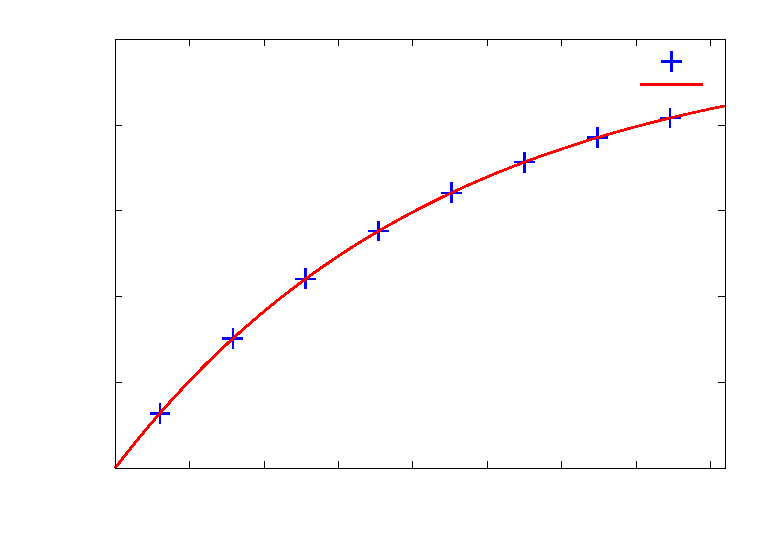
\includegraphics{plots/T1Wasser}}%
    \gplfronttext
  \end{picture}%
\endgroup

    \caption{T1 Messung von Wasser}
\end{figure}

\begin{figure}[H]
    \centering
    % GNUPLOT: LaTeX picture with Postscript
\begingroup
  % Encoding inside the plot.  In the header of your document, this encoding
  % should to defined, e.g., by using
  % \usepackage[cp1252,<other encodings>]{inputenc}
  \inputencoding{cp1252}%
  \makeatletter
  \providecommand\color[2][]{%
    \GenericError{(gnuplot) \space\space\space\@spaces}{%
      Package color not loaded in conjunction with
      terminal option `colourtext'%
    }{See the gnuplot documentation for explanation.%
    }{Either use 'blacktext' in gnuplot or load the package
      color.sty in LaTeX.}%
    \renewcommand\color[2][]{}%
  }%
  \providecommand\includegraphics[2][]{%
    \GenericError{(gnuplot) \space\space\space\@spaces}{%
      Package graphicx or graphics not loaded%
    }{See the gnuplot documentation for explanation.%
    }{The gnuplot epslatex terminal needs graphicx.sty or graphics.sty.}%
    \renewcommand\includegraphics[2][]{}%
  }%
  \providecommand\rotatebox[2]{#2}%
  \@ifundefined{ifGPcolor}{%
    \newif\ifGPcolor
    \GPcolorfalse
  }{}%
  \@ifundefined{ifGPblacktext}{%
    \newif\ifGPblacktext
    \GPblacktexttrue
  }{}%
  % define a \g@addto@macro without @ in the name:
  \let\gplgaddtomacro\g@addto@macro
  % define empty templates for all commands taking text:
  \gdef\gplbacktext{}%
  \gdef\gplfronttext{}%
  \makeatother
  \ifGPblacktext
    % no textcolor at all
    \def\colorrgb#1{}%
    \def\colorgray#1{}%
  \else
    % gray or color?
    \ifGPcolor
      \def\colorrgb#1{\color[rgb]{#1}}%
      \def\colorgray#1{\color[gray]{#1}}%
      \expandafter\def\csname LTw\endcsname{\color{white}}%
      \expandafter\def\csname LTb\endcsname{\color{black}}%
      \expandafter\def\csname LTa\endcsname{\color{black}}%
      \expandafter\def\csname LT0\endcsname{\color[rgb]{1,0,0}}%
      \expandafter\def\csname LT1\endcsname{\color[rgb]{0,1,0}}%
      \expandafter\def\csname LT2\endcsname{\color[rgb]{0,0,1}}%
      \expandafter\def\csname LT3\endcsname{\color[rgb]{1,0,1}}%
      \expandafter\def\csname LT4\endcsname{\color[rgb]{0,1,1}}%
      \expandafter\def\csname LT5\endcsname{\color[rgb]{1,1,0}}%
      \expandafter\def\csname LT6\endcsname{\color[rgb]{0,0,0}}%
      \expandafter\def\csname LT7\endcsname{\color[rgb]{1,0.3,0}}%
      \expandafter\def\csname LT8\endcsname{\color[rgb]{0.5,0.5,0.5}}%
    \else
      % gray
      \def\colorrgb#1{\color{black}}%
      \def\colorgray#1{\color[gray]{#1}}%
      \expandafter\def\csname LTw\endcsname{\color{white}}%
      \expandafter\def\csname LTb\endcsname{\color{black}}%
      \expandafter\def\csname LTa\endcsname{\color{black}}%
      \expandafter\def\csname LT0\endcsname{\color{black}}%
      \expandafter\def\csname LT1\endcsname{\color{black}}%
      \expandafter\def\csname LT2\endcsname{\color{black}}%
      \expandafter\def\csname LT3\endcsname{\color{black}}%
      \expandafter\def\csname LT4\endcsname{\color{black}}%
      \expandafter\def\csname LT5\endcsname{\color{black}}%
      \expandafter\def\csname LT6\endcsname{\color{black}}%
      \expandafter\def\csname LT7\endcsname{\color{black}}%
      \expandafter\def\csname LT8\endcsname{\color{black}}%
    \fi
  \fi
    \setlength{\unitlength}{0.0500bp}%
    \ifx\gptboxheight\undefined%
      \newlength{\gptboxheight}%
      \newlength{\gptboxwidth}%
      \newsavebox{\gptboxtext}%
    \fi%
    \setlength{\fboxrule}{0.5pt}%
    \setlength{\fboxsep}{1pt}%
\begin{picture}(7200.00,5040.00)%
    \gplgaddtomacro\gplbacktext{%
      \csname LTb\endcsname%%
      \put(814,704){\makebox(0,0)[r]{\strut{}$0$}}%
      \put(814,1527){\makebox(0,0)[r]{\strut{}$0.2$}}%
      \put(814,2350){\makebox(0,0)[r]{\strut{}$0.4$}}%
      \put(814,3173){\makebox(0,0)[r]{\strut{}$0.6$}}%
      \put(814,3996){\makebox(0,0)[r]{\strut{}$0.8$}}%
      \put(814,4819){\makebox(0,0)[r]{\strut{}$1$}}%
      \put(946,484){\makebox(0,0){\strut{}$0$}}%
      \put(1922,484){\makebox(0,0){\strut{}$1000$}}%
      \put(2898,484){\makebox(0,0){\strut{}$2000$}}%
      \put(3875,484){\makebox(0,0){\strut{}$3000$}}%
      \put(4851,484){\makebox(0,0){\strut{}$4000$}}%
      \put(5827,484){\makebox(0,0){\strut{}$5000$}}%
      \put(6803,484){\makebox(0,0){\strut{}$6000$}}%
    }%
    \gplgaddtomacro\gplfronttext{%
      \csname LTb\endcsname%%
      \put(308,2761){\rotatebox{-270}{\makebox(0,0){\strut{}Dämpfung $\frac{\text{E}}{\text{E}_0}$}}}%
      \put(3874,154){\makebox(0,0){\strut{}Zeit in $\si{\milli \second}$}}%
      \csname LTb\endcsname%%
      \put(5860,4606){\makebox(0,0)[r]{\strut{}gemessene Datenpunkte für Wasser}}%
      \csname LTb\endcsname%%
      \put(5860,4386){\makebox(0,0)[r]{\strut{}Dämpfungsfit Fit}}%
    }%
    \gplbacktext
    \put(0,0){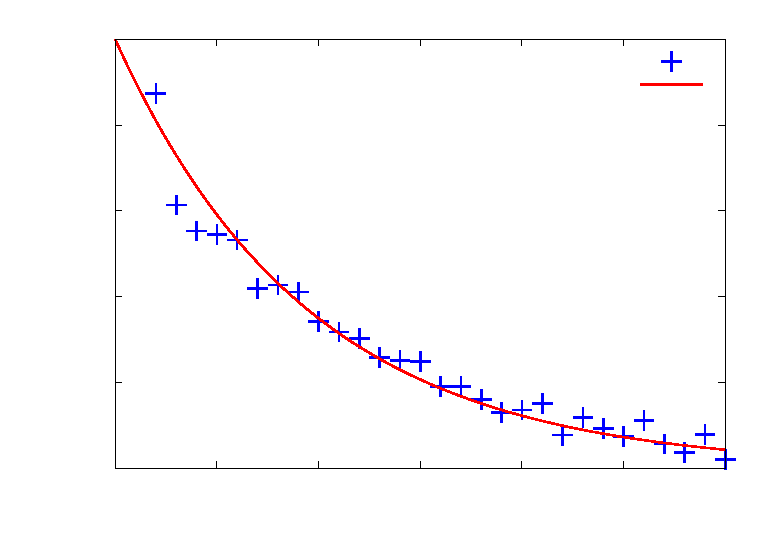
\includegraphics{plots/T2Wasser}}%
    \gplfronttext
  \end{picture}%
\endgroup

    \caption{T2 Messung von Wasser}
\end{figure}

\begin{figure}[H]
    \centering
    % GNUPLOT: LaTeX picture with Postscript
\begingroup
  % Encoding inside the plot.  In the header of your document, this encoding
  % should to defined, e.g., by using
  % \usepackage[cp1252,<other encodings>]{inputenc}
  \inputencoding{cp1252}%
  \makeatletter
  \providecommand\color[2][]{%
    \GenericError{(gnuplot) \space\space\space\@spaces}{%
      Package color not loaded in conjunction with
      terminal option `colourtext'%
    }{See the gnuplot documentation for explanation.%
    }{Either use 'blacktext' in gnuplot or load the package
      color.sty in LaTeX.}%
    \renewcommand\color[2][]{}%
  }%
  \providecommand\includegraphics[2][]{%
    \GenericError{(gnuplot) \space\space\space\@spaces}{%
      Package graphicx or graphics not loaded%
    }{See the gnuplot documentation for explanation.%
    }{The gnuplot epslatex terminal needs graphicx.sty or graphics.sty.}%
    \renewcommand\includegraphics[2][]{}%
  }%
  \providecommand\rotatebox[2]{#2}%
  \@ifundefined{ifGPcolor}{%
    \newif\ifGPcolor
    \GPcolorfalse
  }{}%
  \@ifundefined{ifGPblacktext}{%
    \newif\ifGPblacktext
    \GPblacktexttrue
  }{}%
  % define a \g@addto@macro without @ in the name:
  \let\gplgaddtomacro\g@addto@macro
  % define empty templates for all commands taking text:
  \gdef\gplbacktext{}%
  \gdef\gplfronttext{}%
  \makeatother
  \ifGPblacktext
    % no textcolor at all
    \def\colorrgb#1{}%
    \def\colorgray#1{}%
  \else
    % gray or color?
    \ifGPcolor
      \def\colorrgb#1{\color[rgb]{#1}}%
      \def\colorgray#1{\color[gray]{#1}}%
      \expandafter\def\csname LTw\endcsname{\color{white}}%
      \expandafter\def\csname LTb\endcsname{\color{black}}%
      \expandafter\def\csname LTa\endcsname{\color{black}}%
      \expandafter\def\csname LT0\endcsname{\color[rgb]{1,0,0}}%
      \expandafter\def\csname LT1\endcsname{\color[rgb]{0,1,0}}%
      \expandafter\def\csname LT2\endcsname{\color[rgb]{0,0,1}}%
      \expandafter\def\csname LT3\endcsname{\color[rgb]{1,0,1}}%
      \expandafter\def\csname LT4\endcsname{\color[rgb]{0,1,1}}%
      \expandafter\def\csname LT5\endcsname{\color[rgb]{1,1,0}}%
      \expandafter\def\csname LT6\endcsname{\color[rgb]{0,0,0}}%
      \expandafter\def\csname LT7\endcsname{\color[rgb]{1,0.3,0}}%
      \expandafter\def\csname LT8\endcsname{\color[rgb]{0.5,0.5,0.5}}%
    \else
      % gray
      \def\colorrgb#1{\color{black}}%
      \def\colorgray#1{\color[gray]{#1}}%
      \expandafter\def\csname LTw\endcsname{\color{white}}%
      \expandafter\def\csname LTb\endcsname{\color{black}}%
      \expandafter\def\csname LTa\endcsname{\color{black}}%
      \expandafter\def\csname LT0\endcsname{\color{black}}%
      \expandafter\def\csname LT1\endcsname{\color{black}}%
      \expandafter\def\csname LT2\endcsname{\color{black}}%
      \expandafter\def\csname LT3\endcsname{\color{black}}%
      \expandafter\def\csname LT4\endcsname{\color{black}}%
      \expandafter\def\csname LT5\endcsname{\color{black}}%
      \expandafter\def\csname LT6\endcsname{\color{black}}%
      \expandafter\def\csname LT7\endcsname{\color{black}}%
      \expandafter\def\csname LT8\endcsname{\color{black}}%
    \fi
  \fi
    \setlength{\unitlength}{0.0500bp}%
    \ifx\gptboxheight\undefined%
      \newlength{\gptboxheight}%
      \newlength{\gptboxwidth}%
      \newsavebox{\gptboxtext}%
    \fi%
    \setlength{\fboxrule}{0.5pt}%
    \setlength{\fboxsep}{1pt}%
\begin{picture}(7200.00,5040.00)%
    \gplgaddtomacro\gplbacktext{%
      \csname LTb\endcsname%%
      \put(1474,704){\makebox(0,0)[r]{\strut{}$0.0*10^{0}$}}%
      \put(1474,1292){\makebox(0,0)[r]{\strut{}$5.0*10^{-4}$}}%
      \put(1474,1880){\makebox(0,0)[r]{\strut{}$1.0*10^{-3}$}}%
      \put(1474,2468){\makebox(0,0)[r]{\strut{}$1.5*10^{-3}$}}%
      \put(1474,3055){\makebox(0,0)[r]{\strut{}$2.0*10^{-3}$}}%
      \put(1474,3643){\makebox(0,0)[r]{\strut{}$2.5*10^{-3}$}}%
      \put(1474,4231){\makebox(0,0)[r]{\strut{}$3.0*10^{-3}$}}%
      \put(1474,4819){\makebox(0,0)[r]{\strut{}$3.5*10^{-3}$}}%
      \put(1606,484){\makebox(0,0){\strut{}$0$}}%
      \put(2645,484){\makebox(0,0){\strut{}$1$}}%
      \put(3685,484){\makebox(0,0){\strut{}$2$}}%
      \put(4724,484){\makebox(0,0){\strut{}$3$}}%
      \put(5764,484){\makebox(0,0){\strut{}$4$}}%
      \put(6803,484){\makebox(0,0){\strut{}$5$}}%
    }%
    \gplgaddtomacro\gplfronttext{%
      \csname LTb\endcsname%%
      \put(308,2761){\rotatebox{-270}{\makebox(0,0){\strut{}Kehrwert der Zeit in $\si{\per \second}$}}}%
      \put(4204,154){\makebox(0,0){\strut{}Konzentration in  $\si{\mol \per \meter \tothe{3} }$}}%
      \csname LTb\endcsname%%
      \put(5870,4606){\makebox(0,0)[r]{\strut{}$1/T_{\text{1}}\left([\ce{Cu^2+}]\right)$}}%
      \csname LTb\endcsname%%
      \put(5870,4386){\makebox(0,0)[r]{\strut{}linearer Fit}}%
    }%
    \gplbacktext
    \put(0,0){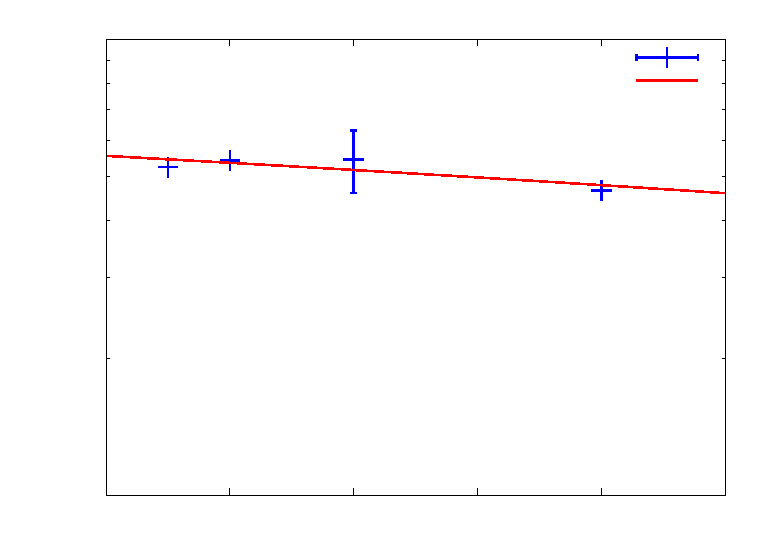
\includegraphics{plots/Relaxivitat_CuT1}}%
    \gplfronttext
  \end{picture}%
\endgroup

    \caption[]{\textcolor{red}{ToD:}Diese Abbildung zeigt die Kehrwerte der vier Relaxationszeiten $T_1$ aufgetragen über den entsprechenden Konzentrationen des im Wasser gelösten Kupersalzes. Mittels eines linearen Fits konnten somit die Relaxivität $r_1$, sowie die Relaxationszeit ohne gelöstes Kontrastmittel nach Gleichung \eqref{eq:relaxivitat} ermittlet werden.
    
    Relaxivitat $r_1$ von Kupfer}
    \label{fig:RelaxCUT1}
\end{figure}

\begin{figure}[H]
    \centering
    % GNUPLOT: LaTeX picture with Postscript
\begingroup
  % Encoding inside the plot.  In the header of your document, this encoding
  % should to defined, e.g., by using
  % \usepackage[cp1252,<other encodings>]{inputenc}
  \inputencoding{cp1252}%
  \makeatletter
  \providecommand\color[2][]{%
    \GenericError{(gnuplot) \space\space\space\@spaces}{%
      Package color not loaded in conjunction with
      terminal option `colourtext'%
    }{See the gnuplot documentation for explanation.%
    }{Either use 'blacktext' in gnuplot or load the package
      color.sty in LaTeX.}%
    \renewcommand\color[2][]{}%
  }%
  \providecommand\includegraphics[2][]{%
    \GenericError{(gnuplot) \space\space\space\@spaces}{%
      Package graphicx or graphics not loaded%
    }{See the gnuplot documentation for explanation.%
    }{The gnuplot epslatex terminal needs graphicx.sty or graphics.sty.}%
    \renewcommand\includegraphics[2][]{}%
  }%
  \providecommand\rotatebox[2]{#2}%
  \@ifundefined{ifGPcolor}{%
    \newif\ifGPcolor
    \GPcolorfalse
  }{}%
  \@ifundefined{ifGPblacktext}{%
    \newif\ifGPblacktext
    \GPblacktexttrue
  }{}%
  % define a \g@addto@macro without @ in the name:
  \let\gplgaddtomacro\g@addto@macro
  % define empty templates for all commands taking text:
  \gdef\gplbacktext{}%
  \gdef\gplfronttext{}%
  \makeatother
  \ifGPblacktext
    % no textcolor at all
    \def\colorrgb#1{}%
    \def\colorgray#1{}%
  \else
    % gray or color?
    \ifGPcolor
      \def\colorrgb#1{\color[rgb]{#1}}%
      \def\colorgray#1{\color[gray]{#1}}%
      \expandafter\def\csname LTw\endcsname{\color{white}}%
      \expandafter\def\csname LTb\endcsname{\color{black}}%
      \expandafter\def\csname LTa\endcsname{\color{black}}%
      \expandafter\def\csname LT0\endcsname{\color[rgb]{1,0,0}}%
      \expandafter\def\csname LT1\endcsname{\color[rgb]{0,1,0}}%
      \expandafter\def\csname LT2\endcsname{\color[rgb]{0,0,1}}%
      \expandafter\def\csname LT3\endcsname{\color[rgb]{1,0,1}}%
      \expandafter\def\csname LT4\endcsname{\color[rgb]{0,1,1}}%
      \expandafter\def\csname LT5\endcsname{\color[rgb]{1,1,0}}%
      \expandafter\def\csname LT6\endcsname{\color[rgb]{0,0,0}}%
      \expandafter\def\csname LT7\endcsname{\color[rgb]{1,0.3,0}}%
      \expandafter\def\csname LT8\endcsname{\color[rgb]{0.5,0.5,0.5}}%
    \else
      % gray
      \def\colorrgb#1{\color{black}}%
      \def\colorgray#1{\color[gray]{#1}}%
      \expandafter\def\csname LTw\endcsname{\color{white}}%
      \expandafter\def\csname LTb\endcsname{\color{black}}%
      \expandafter\def\csname LTa\endcsname{\color{black}}%
      \expandafter\def\csname LT0\endcsname{\color{black}}%
      \expandafter\def\csname LT1\endcsname{\color{black}}%
      \expandafter\def\csname LT2\endcsname{\color{black}}%
      \expandafter\def\csname LT3\endcsname{\color{black}}%
      \expandafter\def\csname LT4\endcsname{\color{black}}%
      \expandafter\def\csname LT5\endcsname{\color{black}}%
      \expandafter\def\csname LT6\endcsname{\color{black}}%
      \expandafter\def\csname LT7\endcsname{\color{black}}%
      \expandafter\def\csname LT8\endcsname{\color{black}}%
    \fi
  \fi
    \setlength{\unitlength}{0.0500bp}%
    \ifx\gptboxheight\undefined%
      \newlength{\gptboxheight}%
      \newlength{\gptboxwidth}%
      \newsavebox{\gptboxtext}%
    \fi%
    \setlength{\fboxrule}{0.5pt}%
    \setlength{\fboxsep}{1pt}%
\begin{picture}(7200.00,5040.00)%
    \gplgaddtomacro\gplbacktext{%
      \csname LTb\endcsname%%
      \put(1474,704){\makebox(0,0)[r]{\strut{}$0.0*10^{0}$}}%
      \put(1474,1218){\makebox(0,0)[r]{\strut{}$5.0*10^{-4}$}}%
      \put(1474,1733){\makebox(0,0)[r]{\strut{}$1.0*10^{-3}$}}%
      \put(1474,2247){\makebox(0,0)[r]{\strut{}$1.5*10^{-3}$}}%
      \put(1474,2762){\makebox(0,0)[r]{\strut{}$2.0*10^{-3}$}}%
      \put(1474,3276){\makebox(0,0)[r]{\strut{}$2.5*10^{-3}$}}%
      \put(1474,3790){\makebox(0,0)[r]{\strut{}$3.0*10^{-3}$}}%
      \put(1474,4305){\makebox(0,0)[r]{\strut{}$3.5*10^{-3}$}}%
      \put(1474,4819){\makebox(0,0)[r]{\strut{}$4.0*10^{-3}$}}%
      \put(1606,484){\makebox(0,0){\strut{}$0$}}%
      \put(2645,484){\makebox(0,0){\strut{}$1$}}%
      \put(3685,484){\makebox(0,0){\strut{}$2$}}%
      \put(4724,484){\makebox(0,0){\strut{}$3$}}%
      \put(5764,484){\makebox(0,0){\strut{}$4$}}%
      \put(6803,484){\makebox(0,0){\strut{}$5$}}%
    }%
    \gplgaddtomacro\gplfronttext{%
      \csname LTb\endcsname%%
      \put(308,2761){\rotatebox{-270}{\makebox(0,0){\strut{}Kehrwert der Zeit in $\si{\per \second}$}}}%
      \put(4204,154){\makebox(0,0){\strut{}Konzentration in  $\si{\mol \per \meter \tothe{3} }$}}%
      \csname LTb\endcsname%%
      \put(5870,4606){\makebox(0,0)[r]{\strut{}$1/T_{\text{2}}\left([\ce{Cu^2+}]\right)$}}%
      \csname LTb\endcsname%%
      \put(5870,4386){\makebox(0,0)[r]{\strut{}linearer Fit}}%
    }%
    \gplbacktext
    \put(0,0){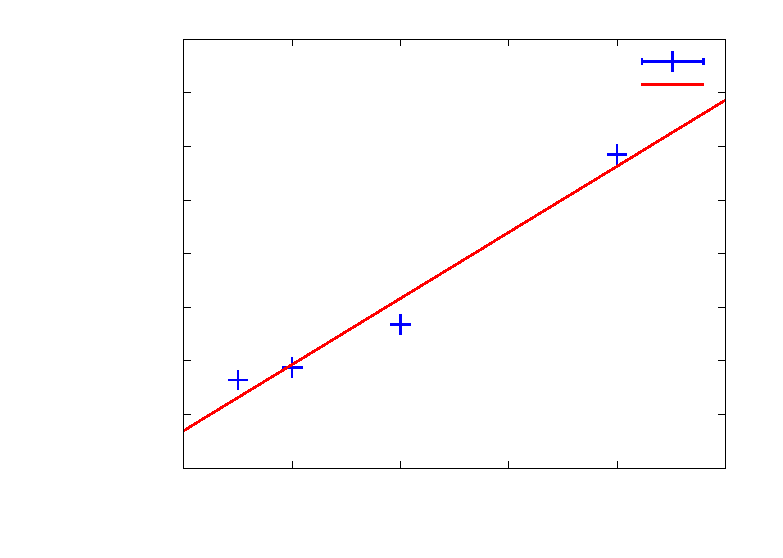
\includegraphics{plots/Relaxivitat_CuT2}}%
    \gplfronttext
  \end{picture}%
\endgroup

    \caption{\textcolor{red}{ToD:}Relaxivitat $r_2$ von Kupfer}
    \label{fig:RelaxCUT2}
\end{figure}

\begin{figure}[H]
    \centering
    % GNUPLOT: LaTeX picture with Postscript
\begingroup
  % Encoding inside the plot.  In the header of your document, this encoding
  % should to defined, e.g., by using
  % \usepackage[cp1252,<other encodings>]{inputenc}
  \inputencoding{cp1252}%
  \makeatletter
  \providecommand\color[2][]{%
    \GenericError{(gnuplot) \space\space\space\@spaces}{%
      Package color not loaded in conjunction with
      terminal option `colourtext'%
    }{See the gnuplot documentation for explanation.%
    }{Either use 'blacktext' in gnuplot or load the package
      color.sty in LaTeX.}%
    \renewcommand\color[2][]{}%
  }%
  \providecommand\includegraphics[2][]{%
    \GenericError{(gnuplot) \space\space\space\@spaces}{%
      Package graphicx or graphics not loaded%
    }{See the gnuplot documentation for explanation.%
    }{The gnuplot epslatex terminal needs graphicx.sty or graphics.sty.}%
    \renewcommand\includegraphics[2][]{}%
  }%
  \providecommand\rotatebox[2]{#2}%
  \@ifundefined{ifGPcolor}{%
    \newif\ifGPcolor
    \GPcolorfalse
  }{}%
  \@ifundefined{ifGPblacktext}{%
    \newif\ifGPblacktext
    \GPblacktexttrue
  }{}%
  % define a \g@addto@macro without @ in the name:
  \let\gplgaddtomacro\g@addto@macro
  % define empty templates for all commands taking text:
  \gdef\gplbacktext{}%
  \gdef\gplfronttext{}%
  \makeatother
  \ifGPblacktext
    % no textcolor at all
    \def\colorrgb#1{}%
    \def\colorgray#1{}%
  \else
    % gray or color?
    \ifGPcolor
      \def\colorrgb#1{\color[rgb]{#1}}%
      \def\colorgray#1{\color[gray]{#1}}%
      \expandafter\def\csname LTw\endcsname{\color{white}}%
      \expandafter\def\csname LTb\endcsname{\color{black}}%
      \expandafter\def\csname LTa\endcsname{\color{black}}%
      \expandafter\def\csname LT0\endcsname{\color[rgb]{1,0,0}}%
      \expandafter\def\csname LT1\endcsname{\color[rgb]{0,1,0}}%
      \expandafter\def\csname LT2\endcsname{\color[rgb]{0,0,1}}%
      \expandafter\def\csname LT3\endcsname{\color[rgb]{1,0,1}}%
      \expandafter\def\csname LT4\endcsname{\color[rgb]{0,1,1}}%
      \expandafter\def\csname LT5\endcsname{\color[rgb]{1,1,0}}%
      \expandafter\def\csname LT6\endcsname{\color[rgb]{0,0,0}}%
      \expandafter\def\csname LT7\endcsname{\color[rgb]{1,0.3,0}}%
      \expandafter\def\csname LT8\endcsname{\color[rgb]{0.5,0.5,0.5}}%
    \else
      % gray
      \def\colorrgb#1{\color{black}}%
      \def\colorgray#1{\color[gray]{#1}}%
      \expandafter\def\csname LTw\endcsname{\color{white}}%
      \expandafter\def\csname LTb\endcsname{\color{black}}%
      \expandafter\def\csname LTa\endcsname{\color{black}}%
      \expandafter\def\csname LT0\endcsname{\color{black}}%
      \expandafter\def\csname LT1\endcsname{\color{black}}%
      \expandafter\def\csname LT2\endcsname{\color{black}}%
      \expandafter\def\csname LT3\endcsname{\color{black}}%
      \expandafter\def\csname LT4\endcsname{\color{black}}%
      \expandafter\def\csname LT5\endcsname{\color{black}}%
      \expandafter\def\csname LT6\endcsname{\color{black}}%
      \expandafter\def\csname LT7\endcsname{\color{black}}%
      \expandafter\def\csname LT8\endcsname{\color{black}}%
    \fi
  \fi
    \setlength{\unitlength}{0.0500bp}%
    \ifx\gptboxheight\undefined%
      \newlength{\gptboxheight}%
      \newlength{\gptboxwidth}%
      \newsavebox{\gptboxtext}%
    \fi%
    \setlength{\fboxrule}{0.5pt}%
    \setlength{\fboxsep}{1pt}%
\begin{picture}(7200.00,5040.00)%
    \gplgaddtomacro\gplbacktext{%
      \csname LTb\endcsname%%
      \put(682,704){\makebox(0,0)[r]{\strut{}$0$}}%
      \put(682,1527){\makebox(0,0)[r]{\strut{}$2$}}%
      \put(682,2350){\makebox(0,0)[r]{\strut{}$4$}}%
      \put(682,3173){\makebox(0,0)[r]{\strut{}$6$}}%
      \put(682,3996){\makebox(0,0)[r]{\strut{}$8$}}%
      \put(682,4819){\makebox(0,0)[r]{\strut{}$10$}}%
      \put(814,484){\makebox(0,0){\strut{}$0$}}%
      \put(2012,484){\makebox(0,0){\strut{}$0.1$}}%
      \put(3210,484){\makebox(0,0){\strut{}$0.2$}}%
      \put(4407,484){\makebox(0,0){\strut{}$0.3$}}%
      \put(5605,484){\makebox(0,0){\strut{}$0.4$}}%
      \put(6803,484){\makebox(0,0){\strut{}$0.5$}}%
    }%
    \gplgaddtomacro\gplfronttext{%
      \csname LTb\endcsname%%
      \put(308,2761){\rotatebox{-270}{\makebox(0,0){\strut{}Kehrwert der Zeit in $\si{\frac{1}{\second}}$}}}%
      \put(3808,154){\makebox(0,0){\strut{}Konzentration in  $\si{\frac{\mol}{\meter \tothe{3}}}$}}%
      \csname LTb\endcsname%%
      \put(5858,4606){\makebox(0,0)[r]{\strut{}$1/T_{\text{1}}\left([\ce{Mn^2+}]\right)$}}%
      \csname LTb\endcsname%%
      \put(5858,4386){\makebox(0,0)[r]{\strut{}linearer Fit}}%
    }%
    \gplbacktext
    \put(0,0){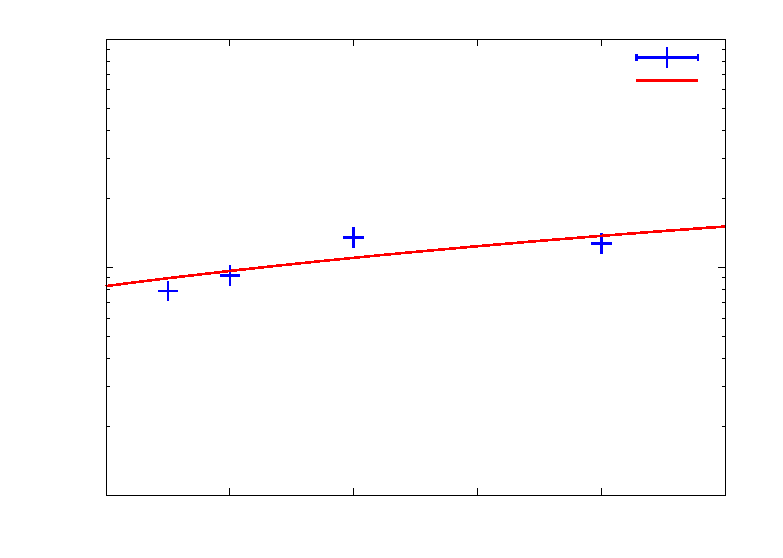
\includegraphics{plots/Relaxivitat_MnT1}}%
    \gplfronttext
  \end{picture}%
\endgroup

    \caption{\textcolor{red}{ToD:}Relaxivitat $r_1$ von Mangan}
    \label{fig:RelaxMNT1}
\end{figure}

\begin{figure}[H]
    \centering
    % GNUPLOT: LaTeX picture with Postscript
\begingroup
  % Encoding inside the plot.  In the header of your document, this encoding
  % should to defined, e.g., by using
  % \usepackage[cp1252,<other encodings>]{inputenc}
  \inputencoding{cp1252}%
  \makeatletter
  \providecommand\color[2][]{%
    \GenericError{(gnuplot) \space\space\space\@spaces}{%
      Package color not loaded in conjunction with
      terminal option `colourtext'%
    }{See the gnuplot documentation for explanation.%
    }{Either use 'blacktext' in gnuplot or load the package
      color.sty in LaTeX.}%
    \renewcommand\color[2][]{}%
  }%
  \providecommand\includegraphics[2][]{%
    \GenericError{(gnuplot) \space\space\space\@spaces}{%
      Package graphicx or graphics not loaded%
    }{See the gnuplot documentation for explanation.%
    }{The gnuplot epslatex terminal needs graphicx.sty or graphics.sty.}%
    \renewcommand\includegraphics[2][]{}%
  }%
  \providecommand\rotatebox[2]{#2}%
  \@ifundefined{ifGPcolor}{%
    \newif\ifGPcolor
    \GPcolorfalse
  }{}%
  \@ifundefined{ifGPblacktext}{%
    \newif\ifGPblacktext
    \GPblacktexttrue
  }{}%
  % define a \g@addto@macro without @ in the name:
  \let\gplgaddtomacro\g@addto@macro
  % define empty templates for all commands taking text:
  \gdef\gplbacktext{}%
  \gdef\gplfronttext{}%
  \makeatother
  \ifGPblacktext
    % no textcolor at all
    \def\colorrgb#1{}%
    \def\colorgray#1{}%
  \else
    % gray or color?
    \ifGPcolor
      \def\colorrgb#1{\color[rgb]{#1}}%
      \def\colorgray#1{\color[gray]{#1}}%
      \expandafter\def\csname LTw\endcsname{\color{white}}%
      \expandafter\def\csname LTb\endcsname{\color{black}}%
      \expandafter\def\csname LTa\endcsname{\color{black}}%
      \expandafter\def\csname LT0\endcsname{\color[rgb]{1,0,0}}%
      \expandafter\def\csname LT1\endcsname{\color[rgb]{0,1,0}}%
      \expandafter\def\csname LT2\endcsname{\color[rgb]{0,0,1}}%
      \expandafter\def\csname LT3\endcsname{\color[rgb]{1,0,1}}%
      \expandafter\def\csname LT4\endcsname{\color[rgb]{0,1,1}}%
      \expandafter\def\csname LT5\endcsname{\color[rgb]{1,1,0}}%
      \expandafter\def\csname LT6\endcsname{\color[rgb]{0,0,0}}%
      \expandafter\def\csname LT7\endcsname{\color[rgb]{1,0.3,0}}%
      \expandafter\def\csname LT8\endcsname{\color[rgb]{0.5,0.5,0.5}}%
    \else
      % gray
      \def\colorrgb#1{\color{black}}%
      \def\colorgray#1{\color[gray]{#1}}%
      \expandafter\def\csname LTw\endcsname{\color{white}}%
      \expandafter\def\csname LTb\endcsname{\color{black}}%
      \expandafter\def\csname LTa\endcsname{\color{black}}%
      \expandafter\def\csname LT0\endcsname{\color{black}}%
      \expandafter\def\csname LT1\endcsname{\color{black}}%
      \expandafter\def\csname LT2\endcsname{\color{black}}%
      \expandafter\def\csname LT3\endcsname{\color{black}}%
      \expandafter\def\csname LT4\endcsname{\color{black}}%
      \expandafter\def\csname LT5\endcsname{\color{black}}%
      \expandafter\def\csname LT6\endcsname{\color{black}}%
      \expandafter\def\csname LT7\endcsname{\color{black}}%
      \expandafter\def\csname LT8\endcsname{\color{black}}%
    \fi
  \fi
    \setlength{\unitlength}{0.0500bp}%
    \ifx\gptboxheight\undefined%
      \newlength{\gptboxheight}%
      \newlength{\gptboxwidth}%
      \newsavebox{\gptboxtext}%
    \fi%
    \setlength{\fboxrule}{0.5pt}%
    \setlength{\fboxsep}{1pt}%
\begin{picture}(7200.00,5040.00)%
    \gplgaddtomacro\gplbacktext{%
      \csname LTb\endcsname%%
      \put(1474,704){\makebox(0,0)[r]{\strut{}$0.0*10^{0}$}}%
      \put(1474,1733){\makebox(0,0)[r]{\strut{}$5.0*10^{-3}$}}%
      \put(1474,2762){\makebox(0,0)[r]{\strut{}$1.0*10^{-2}$}}%
      \put(1474,3790){\makebox(0,0)[r]{\strut{}$1.5*10^{-2}$}}%
      \put(1474,4819){\makebox(0,0)[r]{\strut{}$2.0*10^{-2}$}}%
      \put(1606,484){\makebox(0,0){\strut{}$0$}}%
      \put(2645,484){\makebox(0,0){\strut{}$0.1$}}%
      \put(3685,484){\makebox(0,0){\strut{}$0.2$}}%
      \put(4724,484){\makebox(0,0){\strut{}$0.3$}}%
      \put(5764,484){\makebox(0,0){\strut{}$0.4$}}%
      \put(6803,484){\makebox(0,0){\strut{}$0.5$}}%
    }%
    \gplgaddtomacro\gplfronttext{%
      \csname LTb\endcsname%%
      \put(308,2761){\rotatebox{-270}{\makebox(0,0){\strut{}Kehrwert der Zeit in $\si{\per \second}$}}}%
      \put(4204,154){\makebox(0,0){\strut{}Konzentration in  $\si{\mol \per \meter \tothe{3} }$}}%
      \csname LTb\endcsname%%
      \put(5870,4606){\makebox(0,0)[r]{\strut{}$1/T_{\text{2}}\left([\ce{Mn^2+}]\right)$}}%
      \csname LTb\endcsname%%
      \put(5870,4386){\makebox(0,0)[r]{\strut{}linearer Fit}}%
    }%
    \gplbacktext
    \put(0,0){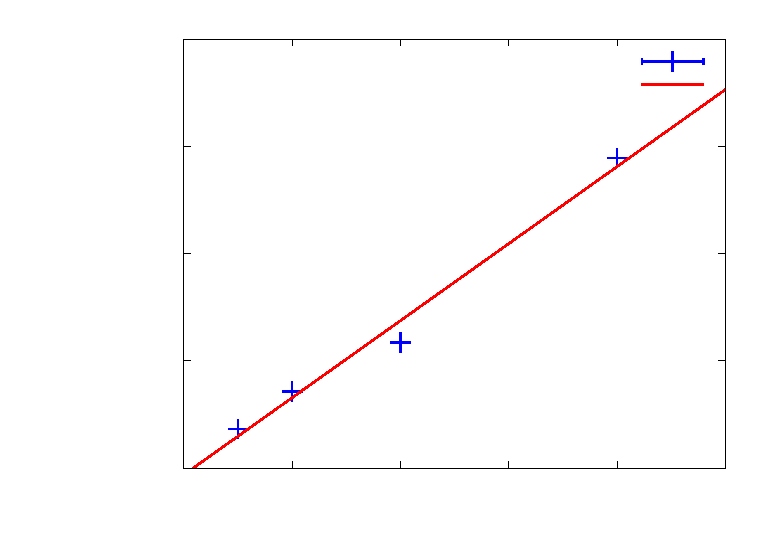
\includegraphics{plots/Relaxivitat_MnT2}}%
    \gplfronttext
  \end{picture}%
\endgroup

    \caption{\textcolor{red}{ToD:}Relaxivitat $r_2$ von Mangan}
    \label{fig:RelaxMNT2}
\end{figure}

\begin{figure}[H]
    \centering
    % GNUPLOT: LaTeX picture with Postscript
\begingroup
  % Encoding inside the plot.  In the header of your document, this encoding
  % should to defined, e.g., by using
  % \usepackage[cp1252,<other encodings>]{inputenc}
  \inputencoding{cp1252}%
  \makeatletter
  \providecommand\color[2][]{%
    \GenericError{(gnuplot) \space\space\space\@spaces}{%
      Package color not loaded in conjunction with
      terminal option `colourtext'%
    }{See the gnuplot documentation for explanation.%
    }{Either use 'blacktext' in gnuplot or load the package
      color.sty in LaTeX.}%
    \renewcommand\color[2][]{}%
  }%
  \providecommand\includegraphics[2][]{%
    \GenericError{(gnuplot) \space\space\space\@spaces}{%
      Package graphicx or graphics not loaded%
    }{See the gnuplot documentation for explanation.%
    }{The gnuplot epslatex terminal needs graphicx.sty or graphics.sty.}%
    \renewcommand\includegraphics[2][]{}%
  }%
  \providecommand\rotatebox[2]{#2}%
  \@ifundefined{ifGPcolor}{%
    \newif\ifGPcolor
    \GPcolorfalse
  }{}%
  \@ifundefined{ifGPblacktext}{%
    \newif\ifGPblacktext
    \GPblacktexttrue
  }{}%
  % define a \g@addto@macro without @ in the name:
  \let\gplgaddtomacro\g@addto@macro
  % define empty templates for all commands taking text:
  \gdef\gplbacktext{}%
  \gdef\gplfronttext{}%
  \makeatother
  \ifGPblacktext
    % no textcolor at all
    \def\colorrgb#1{}%
    \def\colorgray#1{}%
  \else
    % gray or color?
    \ifGPcolor
      \def\colorrgb#1{\color[rgb]{#1}}%
      \def\colorgray#1{\color[gray]{#1}}%
      \expandafter\def\csname LTw\endcsname{\color{white}}%
      \expandafter\def\csname LTb\endcsname{\color{black}}%
      \expandafter\def\csname LTa\endcsname{\color{black}}%
      \expandafter\def\csname LT0\endcsname{\color[rgb]{1,0,0}}%
      \expandafter\def\csname LT1\endcsname{\color[rgb]{0,1,0}}%
      \expandafter\def\csname LT2\endcsname{\color[rgb]{0,0,1}}%
      \expandafter\def\csname LT3\endcsname{\color[rgb]{1,0,1}}%
      \expandafter\def\csname LT4\endcsname{\color[rgb]{0,1,1}}%
      \expandafter\def\csname LT5\endcsname{\color[rgb]{1,1,0}}%
      \expandafter\def\csname LT6\endcsname{\color[rgb]{0,0,0}}%
      \expandafter\def\csname LT7\endcsname{\color[rgb]{1,0.3,0}}%
      \expandafter\def\csname LT8\endcsname{\color[rgb]{0.5,0.5,0.5}}%
    \else
      % gray
      \def\colorrgb#1{\color{black}}%
      \def\colorgray#1{\color[gray]{#1}}%
      \expandafter\def\csname LTw\endcsname{\color{white}}%
      \expandafter\def\csname LTb\endcsname{\color{black}}%
      \expandafter\def\csname LTa\endcsname{\color{black}}%
      \expandafter\def\csname LT0\endcsname{\color{black}}%
      \expandafter\def\csname LT1\endcsname{\color{black}}%
      \expandafter\def\csname LT2\endcsname{\color{black}}%
      \expandafter\def\csname LT3\endcsname{\color{black}}%
      \expandafter\def\csname LT4\endcsname{\color{black}}%
      \expandafter\def\csname LT5\endcsname{\color{black}}%
      \expandafter\def\csname LT6\endcsname{\color{black}}%
      \expandafter\def\csname LT7\endcsname{\color{black}}%
      \expandafter\def\csname LT8\endcsname{\color{black}}%
    \fi
  \fi
    \setlength{\unitlength}{0.0500bp}%
    \ifx\gptboxheight\undefined%
      \newlength{\gptboxheight}%
      \newlength{\gptboxwidth}%
      \newsavebox{\gptboxtext}%
    \fi%
    \setlength{\fboxrule}{0.5pt}%
    \setlength{\fboxsep}{1pt}%
\begin{picture}(7200.00,5040.00)%
    \gplgaddtomacro\gplbacktext{%
      \csname LTb\endcsname%%
      \put(814,704){\makebox(0,0)[r]{\strut{}$0$}}%
      \put(814,1527){\makebox(0,0)[r]{\strut{}$0.2$}}%
      \put(814,2350){\makebox(0,0)[r]{\strut{}$0.4$}}%
      \put(814,3173){\makebox(0,0)[r]{\strut{}$0.6$}}%
      \put(814,3996){\makebox(0,0)[r]{\strut{}$0.8$}}%
      \put(814,4819){\makebox(0,0)[r]{\strut{}$1$}}%
      \put(946,484){\makebox(0,0){\strut{}$0$}}%
      \put(1922,484){\makebox(0,0){\strut{}$1000$}}%
      \put(2898,484){\makebox(0,0){\strut{}$2000$}}%
      \put(3875,484){\makebox(0,0){\strut{}$3000$}}%
      \put(4851,484){\makebox(0,0){\strut{}$4000$}}%
      \put(5827,484){\makebox(0,0){\strut{}$5000$}}%
      \put(6803,484){\makebox(0,0){\strut{}$6000$}}%
    }%
    \gplgaddtomacro\gplfronttext{%
      \csname LTb\endcsname%%
      \put(308,2761){\rotatebox{-270}{\makebox(0,0){\strut{}Dämpfung $\frac{\text{E}}{\text{E}_0}$}}}%
      \put(3874,154){\makebox(0,0){\strut{}Zeit in $\si{\milli \second}$}}%
      \csname LTb\endcsname%%
      \put(5889,3886){\makebox(0,0)[r]{\strut{}$Cu^{2+} \SI{250}{\micro\mole}$}}%
      \csname LTb\endcsname%%
      \put(5889,3666){\makebox(0,0)[r]{\strut{}$Cu^{2+} \SI{500}{\micro\mole}$}}%
      \csname LTb\endcsname%%
      \put(5889,3446){\makebox(0,0)[r]{\strut{}$Cu^{2+} \SI{1000}{\micro\mole}$}}%
      \csname LTb\endcsname%%
      \put(5889,3226){\makebox(0,0)[r]{\strut{}$Cu^{2+} \SI{2000}{\micro\mole}$}}%
      \csname LTb\endcsname%%
      \put(5889,3006){\makebox(0,0)[r]{\strut{}Wasser}}%
    }%
    \gplbacktext
    \put(0,0){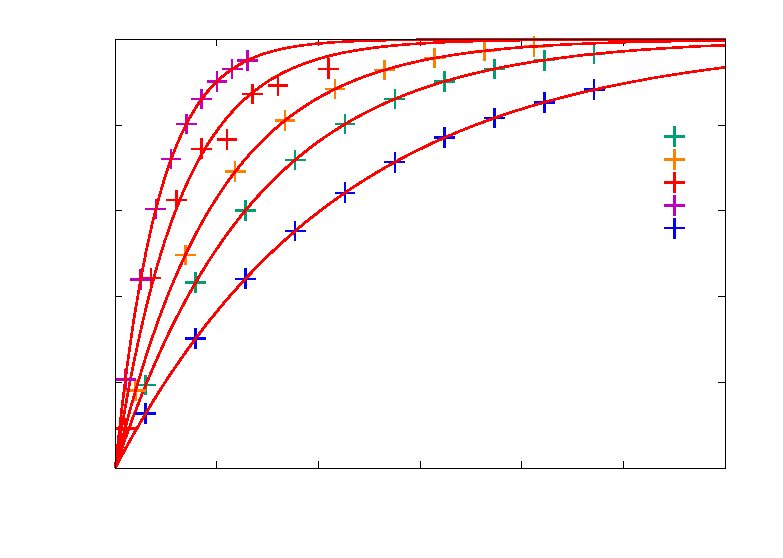
\includegraphics{plots/KupferalleT1}}%
    \gplfronttext
  \end{picture}%
\endgroup

    \caption{\textcolor{red}{ToD:}Alle Messungen T1 Cu2+}
    \label{fig:T1CU}
\end{figure}

\begin{figure}[H]
    \centering
    % GNUPLOT: LaTeX picture with Postscript
\begingroup
  % Encoding inside the plot.  In the header of your document, this encoding
  % should to defined, e.g., by using
  % \usepackage[cp1252,<other encodings>]{inputenc}
  \inputencoding{cp1252}%
  \makeatletter
  \providecommand\color[2][]{%
    \GenericError{(gnuplot) \space\space\space\@spaces}{%
      Package color not loaded in conjunction with
      terminal option `colourtext'%
    }{See the gnuplot documentation for explanation.%
    }{Either use 'blacktext' in gnuplot or load the package
      color.sty in LaTeX.}%
    \renewcommand\color[2][]{}%
  }%
  \providecommand\includegraphics[2][]{%
    \GenericError{(gnuplot) \space\space\space\@spaces}{%
      Package graphicx or graphics not loaded%
    }{See the gnuplot documentation for explanation.%
    }{The gnuplot epslatex terminal needs graphicx.sty or graphics.sty.}%
    \renewcommand\includegraphics[2][]{}%
  }%
  \providecommand\rotatebox[2]{#2}%
  \@ifundefined{ifGPcolor}{%
    \newif\ifGPcolor
    \GPcolorfalse
  }{}%
  \@ifundefined{ifGPblacktext}{%
    \newif\ifGPblacktext
    \GPblacktexttrue
  }{}%
  % define a \g@addto@macro without @ in the name:
  \let\gplgaddtomacro\g@addto@macro
  % define empty templates for all commands taking text:
  \gdef\gplbacktext{}%
  \gdef\gplfronttext{}%
  \makeatother
  \ifGPblacktext
    % no textcolor at all
    \def\colorrgb#1{}%
    \def\colorgray#1{}%
  \else
    % gray or color?
    \ifGPcolor
      \def\colorrgb#1{\color[rgb]{#1}}%
      \def\colorgray#1{\color[gray]{#1}}%
      \expandafter\def\csname LTw\endcsname{\color{white}}%
      \expandafter\def\csname LTb\endcsname{\color{black}}%
      \expandafter\def\csname LTa\endcsname{\color{black}}%
      \expandafter\def\csname LT0\endcsname{\color[rgb]{1,0,0}}%
      \expandafter\def\csname LT1\endcsname{\color[rgb]{0,1,0}}%
      \expandafter\def\csname LT2\endcsname{\color[rgb]{0,0,1}}%
      \expandafter\def\csname LT3\endcsname{\color[rgb]{1,0,1}}%
      \expandafter\def\csname LT4\endcsname{\color[rgb]{0,1,1}}%
      \expandafter\def\csname LT5\endcsname{\color[rgb]{1,1,0}}%
      \expandafter\def\csname LT6\endcsname{\color[rgb]{0,0,0}}%
      \expandafter\def\csname LT7\endcsname{\color[rgb]{1,0.3,0}}%
      \expandafter\def\csname LT8\endcsname{\color[rgb]{0.5,0.5,0.5}}%
    \else
      % gray
      \def\colorrgb#1{\color{black}}%
      \def\colorgray#1{\color[gray]{#1}}%
      \expandafter\def\csname LTw\endcsname{\color{white}}%
      \expandafter\def\csname LTb\endcsname{\color{black}}%
      \expandafter\def\csname LTa\endcsname{\color{black}}%
      \expandafter\def\csname LT0\endcsname{\color{black}}%
      \expandafter\def\csname LT1\endcsname{\color{black}}%
      \expandafter\def\csname LT2\endcsname{\color{black}}%
      \expandafter\def\csname LT3\endcsname{\color{black}}%
      \expandafter\def\csname LT4\endcsname{\color{black}}%
      \expandafter\def\csname LT5\endcsname{\color{black}}%
      \expandafter\def\csname LT6\endcsname{\color{black}}%
      \expandafter\def\csname LT7\endcsname{\color{black}}%
      \expandafter\def\csname LT8\endcsname{\color{black}}%
    \fi
  \fi
    \setlength{\unitlength}{0.0500bp}%
    \ifx\gptboxheight\undefined%
      \newlength{\gptboxheight}%
      \newlength{\gptboxwidth}%
      \newsavebox{\gptboxtext}%
    \fi%
    \setlength{\fboxrule}{0.5pt}%
    \setlength{\fboxsep}{1pt}%
\begin{picture}(7200.00,5040.00)%
    \gplgaddtomacro\gplbacktext{%
      \csname LTb\endcsname%%
      \put(814,704){\makebox(0,0)[r]{\strut{}$0$}}%
      \put(814,1527){\makebox(0,0)[r]{\strut{}$0.2$}}%
      \put(814,2350){\makebox(0,0)[r]{\strut{}$0.4$}}%
      \put(814,3173){\makebox(0,0)[r]{\strut{}$0.6$}}%
      \put(814,3996){\makebox(0,0)[r]{\strut{}$0.8$}}%
      \put(814,4819){\makebox(0,0)[r]{\strut{}$1$}}%
      \put(946,484){\makebox(0,0){\strut{}$0$}}%
      \put(1922,484){\makebox(0,0){\strut{}$1000$}}%
      \put(2898,484){\makebox(0,0){\strut{}$2000$}}%
      \put(3875,484){\makebox(0,0){\strut{}$3000$}}%
      \put(4851,484){\makebox(0,0){\strut{}$4000$}}%
      \put(5827,484){\makebox(0,0){\strut{}$5000$}}%
      \put(6803,484){\makebox(0,0){\strut{}$6000$}}%
    }%
    \gplgaddtomacro\gplfronttext{%
      \csname LTb\endcsname%%
      \put(308,2761){\rotatebox{-270}{\makebox(0,0){\strut{}D\"ampfung $\frac{\text{E}}{\text{E}_0}$}}}%
      \put(3874,154){\makebox(0,0){\strut{}Zeit in $\si{\milli \second}$}}%
      \csname LTb\endcsname%%
      \put(5860,4606){\makebox(0,0)[r]{\strut{}$Cu^{2+} \SI{250}{\micro\mole}$}}%
      \csname LTb\endcsname%%
      \put(5860,4386){\makebox(0,0)[r]{\strut{}$Cu^{2+} \SI{1000}{\micro\mole}$}}%
      \csname LTb\endcsname%%
      \put(5860,4166){\makebox(0,0)[r]{\strut{}$Cu^{2+} \SI{250}{\micro\mole}$}}%
      \csname LTb\endcsname%%
      \put(5860,3946){\makebox(0,0)[r]{\strut{}$Cu^{2+} \SI{2000}{\micro\mole}$}}%
      \csname LTb\endcsname%%
      \put(5860,3726){\makebox(0,0)[r]{\strut{}Wasser}}%
    }%
    \gplbacktext
    \put(0,0){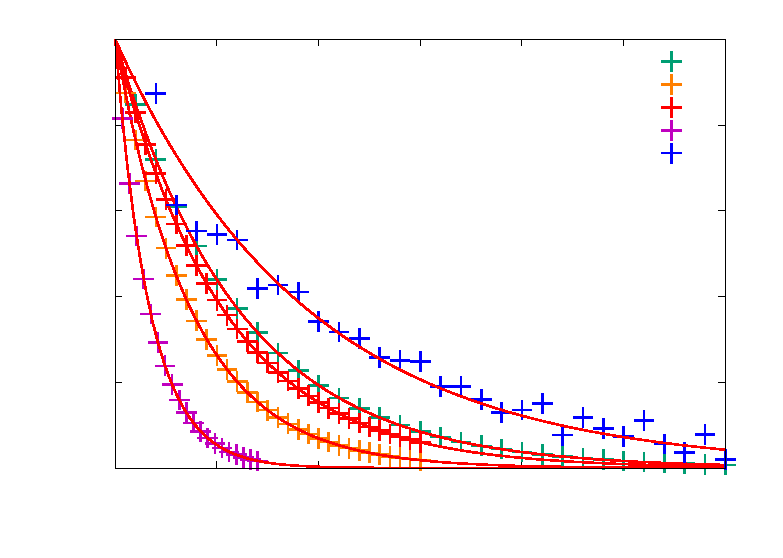
\includegraphics{plots/KupferalleT2}}%
    \gplfronttext
  \end{picture}%
\endgroup

    \caption{\textcolor{red}{ToD:}Alle Messungen T2Cu2+}
    \label{fig:T2CU}
\end{figure}

\begin{figure}[H]
    \centering
    % GNUPLOT: LaTeX picture with Postscript
\begingroup
  % Encoding inside the plot.  In the header of your document, this encoding
  % should to defined, e.g., by using
  % \usepackage[cp1252,<other encodings>]{inputenc}
  \inputencoding{cp1252}%
  \makeatletter
  \providecommand\color[2][]{%
    \GenericError{(gnuplot) \space\space\space\@spaces}{%
      Package color not loaded in conjunction with
      terminal option `colourtext'%
    }{See the gnuplot documentation for explanation.%
    }{Either use 'blacktext' in gnuplot or load the package
      color.sty in LaTeX.}%
    \renewcommand\color[2][]{}%
  }%
  \providecommand\includegraphics[2][]{%
    \GenericError{(gnuplot) \space\space\space\@spaces}{%
      Package graphicx or graphics not loaded%
    }{See the gnuplot documentation for explanation.%
    }{The gnuplot epslatex terminal needs graphicx.sty or graphics.sty.}%
    \renewcommand\includegraphics[2][]{}%
  }%
  \providecommand\rotatebox[2]{#2}%
  \@ifundefined{ifGPcolor}{%
    \newif\ifGPcolor
    \GPcolorfalse
  }{}%
  \@ifundefined{ifGPblacktext}{%
    \newif\ifGPblacktext
    \GPblacktexttrue
  }{}%
  % define a \g@addto@macro without @ in the name:
  \let\gplgaddtomacro\g@addto@macro
  % define empty templates for all commands taking text:
  \gdef\gplbacktext{}%
  \gdef\gplfronttext{}%
  \makeatother
  \ifGPblacktext
    % no textcolor at all
    \def\colorrgb#1{}%
    \def\colorgray#1{}%
  \else
    % gray or color?
    \ifGPcolor
      \def\colorrgb#1{\color[rgb]{#1}}%
      \def\colorgray#1{\color[gray]{#1}}%
      \expandafter\def\csname LTw\endcsname{\color{white}}%
      \expandafter\def\csname LTb\endcsname{\color{black}}%
      \expandafter\def\csname LTa\endcsname{\color{black}}%
      \expandafter\def\csname LT0\endcsname{\color[rgb]{1,0,0}}%
      \expandafter\def\csname LT1\endcsname{\color[rgb]{0,1,0}}%
      \expandafter\def\csname LT2\endcsname{\color[rgb]{0,0,1}}%
      \expandafter\def\csname LT3\endcsname{\color[rgb]{1,0,1}}%
      \expandafter\def\csname LT4\endcsname{\color[rgb]{0,1,1}}%
      \expandafter\def\csname LT5\endcsname{\color[rgb]{1,1,0}}%
      \expandafter\def\csname LT6\endcsname{\color[rgb]{0,0,0}}%
      \expandafter\def\csname LT7\endcsname{\color[rgb]{1,0.3,0}}%
      \expandafter\def\csname LT8\endcsname{\color[rgb]{0.5,0.5,0.5}}%
    \else
      % gray
      \def\colorrgb#1{\color{black}}%
      \def\colorgray#1{\color[gray]{#1}}%
      \expandafter\def\csname LTw\endcsname{\color{white}}%
      \expandafter\def\csname LTb\endcsname{\color{black}}%
      \expandafter\def\csname LTa\endcsname{\color{black}}%
      \expandafter\def\csname LT0\endcsname{\color{black}}%
      \expandafter\def\csname LT1\endcsname{\color{black}}%
      \expandafter\def\csname LT2\endcsname{\color{black}}%
      \expandafter\def\csname LT3\endcsname{\color{black}}%
      \expandafter\def\csname LT4\endcsname{\color{black}}%
      \expandafter\def\csname LT5\endcsname{\color{black}}%
      \expandafter\def\csname LT6\endcsname{\color{black}}%
      \expandafter\def\csname LT7\endcsname{\color{black}}%
      \expandafter\def\csname LT8\endcsname{\color{black}}%
    \fi
  \fi
    \setlength{\unitlength}{0.0500bp}%
    \ifx\gptboxheight\undefined%
      \newlength{\gptboxheight}%
      \newlength{\gptboxwidth}%
      \newsavebox{\gptboxtext}%
    \fi%
    \setlength{\fboxrule}{0.5pt}%
    \setlength{\fboxsep}{1pt}%
\begin{picture}(7200.00,5040.00)%
    \gplgaddtomacro\gplbacktext{%
      \csname LTb\endcsname%%
      \put(814,704){\makebox(0,0)[r]{\strut{}$0$}}%
      \put(814,1527){\makebox(0,0)[r]{\strut{}$0.2$}}%
      \put(814,2350){\makebox(0,0)[r]{\strut{}$0.4$}}%
      \put(814,3173){\makebox(0,0)[r]{\strut{}$0.6$}}%
      \put(814,3996){\makebox(0,0)[r]{\strut{}$0.8$}}%
      \put(814,4819){\makebox(0,0)[r]{\strut{}$1$}}%
      \put(946,484){\makebox(0,0){\strut{}$0$}}%
      \put(1922,484){\makebox(0,0){\strut{}$1000$}}%
      \put(2898,484){\makebox(0,0){\strut{}$2000$}}%
      \put(3875,484){\makebox(0,0){\strut{}$3000$}}%
      \put(4851,484){\makebox(0,0){\strut{}$4000$}}%
      \put(5827,484){\makebox(0,0){\strut{}$5000$}}%
      \put(6803,484){\makebox(0,0){\strut{}$6000$}}%
    }%
    \gplgaddtomacro\gplfronttext{%
      \csname LTb\endcsname%%
      \put(198,2761){\rotatebox{-270}{\makebox(0,0){\strut{}D\"ampfung $\frac{\text{E}}{\text{E}_0}$}}}%
      \put(3874,154){\makebox(0,0){\strut{}Zeit in $\si{\milli \second}$}}%
      \csname LTb\endcsname%%
      \put(5860,3680){\makebox(0,0)[r]{\strut{}$Mn^{2+} \SI{25}{\micro\mole}$}}%
      \csname LTb\endcsname%%
      \put(5860,3460){\makebox(0,0)[r]{\strut{}$Mn^{2+} \SI{50}{\micro\mole}$}}%
      \csname LTb\endcsname%%
      \put(5860,3240){\makebox(0,0)[r]{\strut{}$Mn^{2+} \SI{100}{\micro\mole}$}}%
      \csname LTb\endcsname%%
      \put(5860,3020){\makebox(0,0)[r]{\strut{}$Mn^{2+} \SI{200}{\micro\mole}$}}%
      \csname LTb\endcsname%%
      \put(5860,2800){\makebox(0,0)[r]{\strut{}Wasser}}%
    }%
    \gplbacktext
    \put(0,0){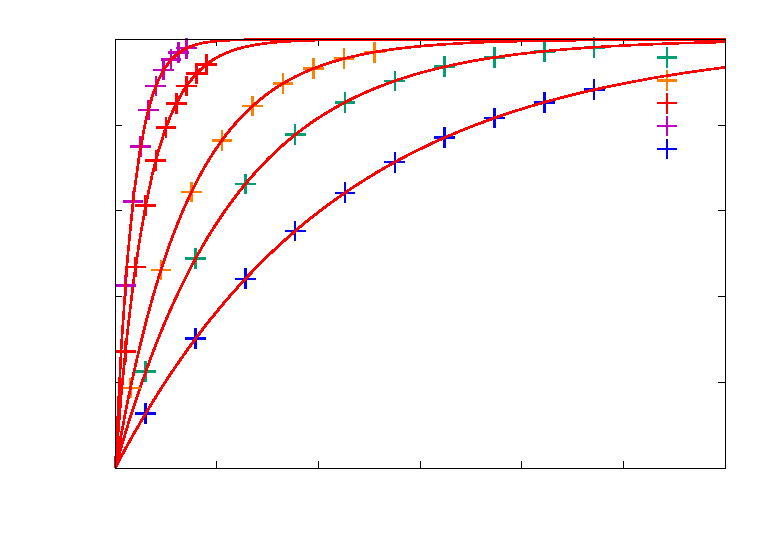
\includegraphics{plots/ManganalleT1}}%
    \gplfronttext
  \end{picture}%
\endgroup

    \caption{\textcolor{red}{ToD:}Alle Messungen T1Mn2+}
    \label{fig:T1Mn}
\end{figure}

\begin{figure}[H]
    \centering
    % GNUPLOT: LaTeX picture with Postscript
\begingroup
  % Encoding inside the plot.  In the header of your document, this encoding
  % should to defined, e.g., by using
  % \usepackage[cp1252,<other encodings>]{inputenc}
  \inputencoding{cp1252}%
  \makeatletter
  \providecommand\color[2][]{%
    \GenericError{(gnuplot) \space\space\space\@spaces}{%
      Package color not loaded in conjunction with
      terminal option `colourtext'%
    }{See the gnuplot documentation for explanation.%
    }{Either use 'blacktext' in gnuplot or load the package
      color.sty in LaTeX.}%
    \renewcommand\color[2][]{}%
  }%
  \providecommand\includegraphics[2][]{%
    \GenericError{(gnuplot) \space\space\space\@spaces}{%
      Package graphicx or graphics not loaded%
    }{See the gnuplot documentation for explanation.%
    }{The gnuplot epslatex terminal needs graphicx.sty or graphics.sty.}%
    \renewcommand\includegraphics[2][]{}%
  }%
  \providecommand\rotatebox[2]{#2}%
  \@ifundefined{ifGPcolor}{%
    \newif\ifGPcolor
    \GPcolorfalse
  }{}%
  \@ifundefined{ifGPblacktext}{%
    \newif\ifGPblacktext
    \GPblacktexttrue
  }{}%
  % define a \g@addto@macro without @ in the name:
  \let\gplgaddtomacro\g@addto@macro
  % define empty templates for all commands taking text:
  \gdef\gplbacktext{}%
  \gdef\gplfronttext{}%
  \makeatother
  \ifGPblacktext
    % no textcolor at all
    \def\colorrgb#1{}%
    \def\colorgray#1{}%
  \else
    % gray or color?
    \ifGPcolor
      \def\colorrgb#1{\color[rgb]{#1}}%
      \def\colorgray#1{\color[gray]{#1}}%
      \expandafter\def\csname LTw\endcsname{\color{white}}%
      \expandafter\def\csname LTb\endcsname{\color{black}}%
      \expandafter\def\csname LTa\endcsname{\color{black}}%
      \expandafter\def\csname LT0\endcsname{\color[rgb]{1,0,0}}%
      \expandafter\def\csname LT1\endcsname{\color[rgb]{0,1,0}}%
      \expandafter\def\csname LT2\endcsname{\color[rgb]{0,0,1}}%
      \expandafter\def\csname LT3\endcsname{\color[rgb]{1,0,1}}%
      \expandafter\def\csname LT4\endcsname{\color[rgb]{0,1,1}}%
      \expandafter\def\csname LT5\endcsname{\color[rgb]{1,1,0}}%
      \expandafter\def\csname LT6\endcsname{\color[rgb]{0,0,0}}%
      \expandafter\def\csname LT7\endcsname{\color[rgb]{1,0.3,0}}%
      \expandafter\def\csname LT8\endcsname{\color[rgb]{0.5,0.5,0.5}}%
    \else
      % gray
      \def\colorrgb#1{\color{black}}%
      \def\colorgray#1{\color[gray]{#1}}%
      \expandafter\def\csname LTw\endcsname{\color{white}}%
      \expandafter\def\csname LTb\endcsname{\color{black}}%
      \expandafter\def\csname LTa\endcsname{\color{black}}%
      \expandafter\def\csname LT0\endcsname{\color{black}}%
      \expandafter\def\csname LT1\endcsname{\color{black}}%
      \expandafter\def\csname LT2\endcsname{\color{black}}%
      \expandafter\def\csname LT3\endcsname{\color{black}}%
      \expandafter\def\csname LT4\endcsname{\color{black}}%
      \expandafter\def\csname LT5\endcsname{\color{black}}%
      \expandafter\def\csname LT6\endcsname{\color{black}}%
      \expandafter\def\csname LT7\endcsname{\color{black}}%
      \expandafter\def\csname LT8\endcsname{\color{black}}%
    \fi
  \fi
    \setlength{\unitlength}{0.0500bp}%
    \ifx\gptboxheight\undefined%
      \newlength{\gptboxheight}%
      \newlength{\gptboxwidth}%
      \newsavebox{\gptboxtext}%
    \fi%
    \setlength{\fboxrule}{0.5pt}%
    \setlength{\fboxsep}{1pt}%
\begin{picture}(7200.00,5040.00)%
    \gplgaddtomacro\gplbacktext{%
      \csname LTb\endcsname%%
      \put(814,704){\makebox(0,0)[r]{\strut{}$0$}}%
      \put(814,1527){\makebox(0,0)[r]{\strut{}$0.2$}}%
      \put(814,2350){\makebox(0,0)[r]{\strut{}$0.4$}}%
      \put(814,3173){\makebox(0,0)[r]{\strut{}$0.6$}}%
      \put(814,3996){\makebox(0,0)[r]{\strut{}$0.8$}}%
      \put(814,4819){\makebox(0,0)[r]{\strut{}$1$}}%
      \put(946,484){\makebox(0,0){\strut{}$0$}}%
      \put(1922,484){\makebox(0,0){\strut{}$1000$}}%
      \put(2898,484){\makebox(0,0){\strut{}$2000$}}%
      \put(3875,484){\makebox(0,0){\strut{}$3000$}}%
      \put(4851,484){\makebox(0,0){\strut{}$4000$}}%
      \put(5827,484){\makebox(0,0){\strut{}$5000$}}%
      \put(6803,484){\makebox(0,0){\strut{}$6000$}}%
    }%
    \gplgaddtomacro\gplfronttext{%
      \csname LTb\endcsname%%
      \put(198,2761){\rotatebox{-270}{\makebox(0,0){\strut{}D\"ampfung $\frac{\text{E}}{\text{E}_0}$}}}%
      \put(3874,154){\makebox(0,0){\strut{}Zeit in $\si{\milli \second}$}}%
      \csname LTb\endcsname%%
      \put(5860,4606){\makebox(0,0)[r]{\strut{}$Mn^{2+} \SI{25}{\micro\mole}$}}%
      \csname LTb\endcsname%%
      \put(5860,4386){\makebox(0,0)[r]{\strut{}$Mn^{2+} \SI{100}{\micro\mole}$}}%
      \csname LTb\endcsname%%
      \put(5860,4166){\makebox(0,0)[r]{\strut{}$Mn^{2+} \SI{25}{\micro\mole}$}}%
      \csname LTb\endcsname%%
      \put(5860,3946){\makebox(0,0)[r]{\strut{}$Mn^{2+} \SI{200}{\micro\mole}$}}%
      \csname LTb\endcsname%%
      \put(5860,3726){\makebox(0,0)[r]{\strut{}Wasser}}%
    }%
    \gplbacktext
    \put(0,0){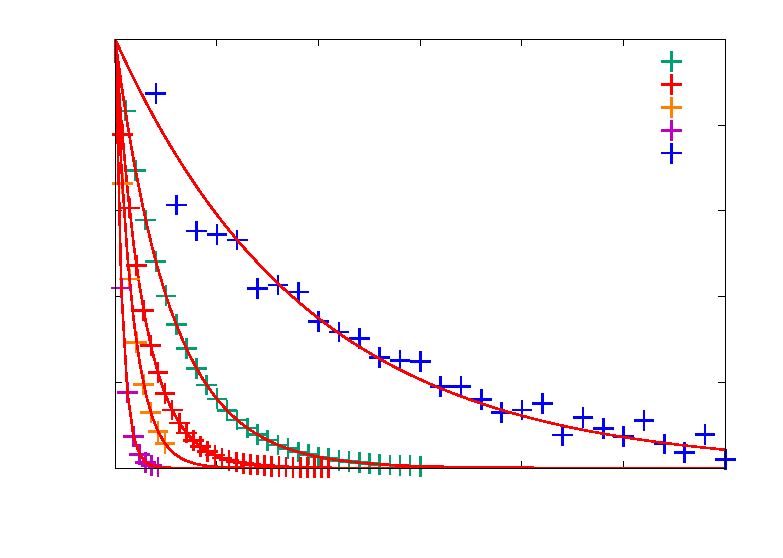
\includegraphics{plots/ManganalleT2}}%
    \gplfronttext
  \end{picture}%
\endgroup

    \caption{\textcolor{red}{ToD:}Alle Messungen T2MN2+}
    \label{fig:T2M}
\end{figure}

\begin{figure}[H]
    \centering
    % GNUPLOT: LaTeX picture with Postscript
\begingroup
  % Encoding inside the plot.  In the header of your document, this encoding
  % should to defined, e.g., by using
  % \usepackage[cp1252,<other encodings>]{inputenc}
  \inputencoding{cp1252}%
  \makeatletter
  \providecommand\color[2][]{%
    \GenericError{(gnuplot) \space\space\space\@spaces}{%
      Package color not loaded in conjunction with
      terminal option `colourtext'%
    }{See the gnuplot documentation for explanation.%
    }{Either use 'blacktext' in gnuplot or load the package
      color.sty in LaTeX.}%
    \renewcommand\color[2][]{}%
  }%
  \providecommand\includegraphics[2][]{%
    \GenericError{(gnuplot) \space\space\space\@spaces}{%
      Package graphicx or graphics not loaded%
    }{See the gnuplot documentation for explanation.%
    }{The gnuplot epslatex terminal needs graphicx.sty or graphics.sty.}%
    \renewcommand\includegraphics[2][]{}%
  }%
  \providecommand\rotatebox[2]{#2}%
  \@ifundefined{ifGPcolor}{%
    \newif\ifGPcolor
    \GPcolorfalse
  }{}%
  \@ifundefined{ifGPblacktext}{%
    \newif\ifGPblacktext
    \GPblacktexttrue
  }{}%
  % define a \g@addto@macro without @ in the name:
  \let\gplgaddtomacro\g@addto@macro
  % define empty templates for all commands taking text:
  \gdef\gplbacktext{}%
  \gdef\gplfronttext{}%
  \makeatother
  \ifGPblacktext
    % no textcolor at all
    \def\colorrgb#1{}%
    \def\colorgray#1{}%
  \else
    % gray or color?
    \ifGPcolor
      \def\colorrgb#1{\color[rgb]{#1}}%
      \def\colorgray#1{\color[gray]{#1}}%
      \expandafter\def\csname LTw\endcsname{\color{white}}%
      \expandafter\def\csname LTb\endcsname{\color{black}}%
      \expandafter\def\csname LTa\endcsname{\color{black}}%
      \expandafter\def\csname LT0\endcsname{\color[rgb]{1,0,0}}%
      \expandafter\def\csname LT1\endcsname{\color[rgb]{0,1,0}}%
      \expandafter\def\csname LT2\endcsname{\color[rgb]{0,0,1}}%
      \expandafter\def\csname LT3\endcsname{\color[rgb]{1,0,1}}%
      \expandafter\def\csname LT4\endcsname{\color[rgb]{0,1,1}}%
      \expandafter\def\csname LT5\endcsname{\color[rgb]{1,1,0}}%
      \expandafter\def\csname LT6\endcsname{\color[rgb]{0,0,0}}%
      \expandafter\def\csname LT7\endcsname{\color[rgb]{1,0.3,0}}%
      \expandafter\def\csname LT8\endcsname{\color[rgb]{0.5,0.5,0.5}}%
    \else
      % gray
      \def\colorrgb#1{\color{black}}%
      \def\colorgray#1{\color[gray]{#1}}%
      \expandafter\def\csname LTw\endcsname{\color{white}}%
      \expandafter\def\csname LTb\endcsname{\color{black}}%
      \expandafter\def\csname LTa\endcsname{\color{black}}%
      \expandafter\def\csname LT0\endcsname{\color{black}}%
      \expandafter\def\csname LT1\endcsname{\color{black}}%
      \expandafter\def\csname LT2\endcsname{\color{black}}%
      \expandafter\def\csname LT3\endcsname{\color{black}}%
      \expandafter\def\csname LT4\endcsname{\color{black}}%
      \expandafter\def\csname LT5\endcsname{\color{black}}%
      \expandafter\def\csname LT6\endcsname{\color{black}}%
      \expandafter\def\csname LT7\endcsname{\color{black}}%
      \expandafter\def\csname LT8\endcsname{\color{black}}%
    \fi
  \fi
    \setlength{\unitlength}{0.0500bp}%
    \ifx\gptboxheight\undefined%
      \newlength{\gptboxheight}%
      \newlength{\gptboxwidth}%
      \newsavebox{\gptboxtext}%
    \fi%
    \setlength{\fboxrule}{0.5pt}%
    \setlength{\fboxsep}{1pt}%
\begin{picture}(7200.00,5040.00)%
    \gplgaddtomacro\gplbacktext{%
      \csname LTb\endcsname%%
      \put(682,704){\makebox(0,0)[r]{\strut{}$0$}}%
      \put(682,1390){\makebox(0,0)[r]{\strut{}$5$}}%
      \put(682,2076){\makebox(0,0)[r]{\strut{}$10$}}%
      \put(682,2762){\makebox(0,0)[r]{\strut{}$15$}}%
      \put(682,3447){\makebox(0,0)[r]{\strut{}$20$}}%
      \put(682,4133){\makebox(0,0)[r]{\strut{}$25$}}%
      \put(682,4819){\makebox(0,0)[r]{\strut{}$30$}}%
      \put(814,484){\makebox(0,0){\strut{}$1800$}}%
      \put(2012,484){\makebox(0,0){\strut{}$1820$}}%
      \put(3210,484){\makebox(0,0){\strut{}$1840$}}%
      \put(4407,484){\makebox(0,0){\strut{}$1860$}}%
      \put(5605,484){\makebox(0,0){\strut{}$1880$}}%
      \put(6803,484){\makebox(0,0){\strut{}$1900$}}%
    }%
    \gplgaddtomacro\gplfronttext{%
      \csname LTb\endcsname%%
      \put(198,2761){\rotatebox{-270}{\makebox(0,0){\strut{}Amplitude in $\si{\frac{\mu \volt}{\hertz}}$}}}%
      \put(3808,154){\makebox(0,0){\strut{}Frequenz in $\si{\hertz}$}}%
      \csname LTb\endcsname%%
      \put(5816,4646){\makebox(0,0)[r]{\strut{}Signal von $Cu^{2+}$ $T_{1}$ mit $\SI{250}{\micro\mole}$}}%
      \csname LTb\endcsname%%
      \put(5816,4426){\makebox(0,0)[r]{\strut{}Signal von $Cu^{2+}$ $T_{1}$ $\SI{500}{\micro\mole}$}}%
    }%
    \gplbacktext
    \put(0,0){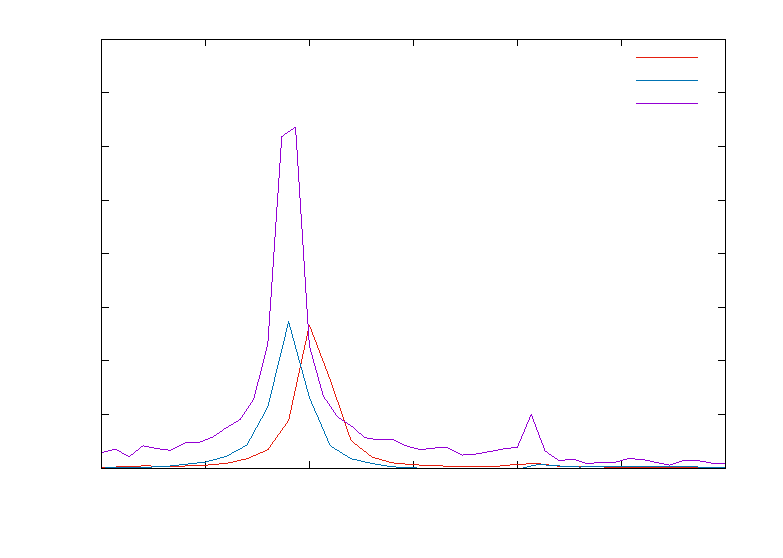
\includegraphics{plots/SignalkontrastT1}}%
    \gplfronttext
  \end{picture}%
\endgroup

    \caption{Die T1 Signale bei der jeweiligen Konzentration}
    \label{fig:T1Signalkontrast}
\end{figure}

\begin{table}[H]
    \centering
    \caption{Relaxivitäten von Kupfer und Mangan.}
    \begin{tabular}{|l||r|r|r|r|} \hline
        Kontrastmittel & $r_{1}$ in $\si{\frac{\mol}{\metre \cubed \second}}$    &  $T_{1}$ in $\si{\second}$ & $r_{2}$ in $\si{\frac{\mol}{\metre \cubed \second}}$ & $T_{2}$ in $\si{\second}$  \\ \hline \hline
        Kupfer & $\SI{0.454 \pm 0.031}{}$   & $\SI{1.84 \pm 0.24}{}$    & $\SI{0.617 \pm 0.084}{}$   & $\SI{2.9  \pm 1.6}{}$ \\ \hline
        Mangan & $\SI{13.65 \pm 0.84}{}$    & $\SI{5.7 \pm 6.3}{}$      & $\SI{35.9 \pm 3.1}{}$  & $\SI{-3.2 \pm 7.5}{}$ \\ \hline
    \end{tabular} 
    \label{tab:Relaxivitat} 
\end{table}
    
    % \begin{figure}[H]
    %     \centering
    %     % GNUPLOT: LaTeX picture with Postscript
\begingroup
  % Encoding inside the plot.  In the header of your document, this encoding
  % should to defined, e.g., by using
  % \usepackage[cp1252,<other encodings>]{inputenc}
  \inputencoding{cp1252}%
  \makeatletter
  \providecommand\color[2][]{%
    \GenericError{(gnuplot) \space\space\space\@spaces}{%
      Package color not loaded in conjunction with
      terminal option `colourtext'%
    }{See the gnuplot documentation for explanation.%
    }{Either use 'blacktext' in gnuplot or load the package
      color.sty in LaTeX.}%
    \renewcommand\color[2][]{}%
  }%
  \providecommand\includegraphics[2][]{%
    \GenericError{(gnuplot) \space\space\space\@spaces}{%
      Package graphicx or graphics not loaded%
    }{See the gnuplot documentation for explanation.%
    }{The gnuplot epslatex terminal needs graphicx.sty or graphics.sty.}%
    \renewcommand\includegraphics[2][]{}%
  }%
  \providecommand\rotatebox[2]{#2}%
  \@ifundefined{ifGPcolor}{%
    \newif\ifGPcolor
    \GPcolorfalse
  }{}%
  \@ifundefined{ifGPblacktext}{%
    \newif\ifGPblacktext
    \GPblacktexttrue
  }{}%
  % define a \g@addto@macro without @ in the name:
  \let\gplgaddtomacro\g@addto@macro
  % define empty templates for all commands taking text:
  \gdef\gplbacktext{}%
  \gdef\gplfronttext{}%
  \makeatother
  \ifGPblacktext
    % no textcolor at all
    \def\colorrgb#1{}%
    \def\colorgray#1{}%
  \else
    % gray or color?
    \ifGPcolor
      \def\colorrgb#1{\color[rgb]{#1}}%
      \def\colorgray#1{\color[gray]{#1}}%
      \expandafter\def\csname LTw\endcsname{\color{white}}%
      \expandafter\def\csname LTb\endcsname{\color{black}}%
      \expandafter\def\csname LTa\endcsname{\color{black}}%
      \expandafter\def\csname LT0\endcsname{\color[rgb]{1,0,0}}%
      \expandafter\def\csname LT1\endcsname{\color[rgb]{0,1,0}}%
      \expandafter\def\csname LT2\endcsname{\color[rgb]{0,0,1}}%
      \expandafter\def\csname LT3\endcsname{\color[rgb]{1,0,1}}%
      \expandafter\def\csname LT4\endcsname{\color[rgb]{0,1,1}}%
      \expandafter\def\csname LT5\endcsname{\color[rgb]{1,1,0}}%
      \expandafter\def\csname LT6\endcsname{\color[rgb]{0,0,0}}%
      \expandafter\def\csname LT7\endcsname{\color[rgb]{1,0.3,0}}%
      \expandafter\def\csname LT8\endcsname{\color[rgb]{0.5,0.5,0.5}}%
    \else
      % gray
      \def\colorrgb#1{\color{black}}%
      \def\colorgray#1{\color[gray]{#1}}%
      \expandafter\def\csname LTw\endcsname{\color{white}}%
      \expandafter\def\csname LTb\endcsname{\color{black}}%
      \expandafter\def\csname LTa\endcsname{\color{black}}%
      \expandafter\def\csname LT0\endcsname{\color{black}}%
      \expandafter\def\csname LT1\endcsname{\color{black}}%
      \expandafter\def\csname LT2\endcsname{\color{black}}%
      \expandafter\def\csname LT3\endcsname{\color{black}}%
      \expandafter\def\csname LT4\endcsname{\color{black}}%
      \expandafter\def\csname LT5\endcsname{\color{black}}%
      \expandafter\def\csname LT6\endcsname{\color{black}}%
      \expandafter\def\csname LT7\endcsname{\color{black}}%
      \expandafter\def\csname LT8\endcsname{\color{black}}%
    \fi
  \fi
    \setlength{\unitlength}{0.0500bp}%
    \ifx\gptboxheight\undefined%
      \newlength{\gptboxheight}%
      \newlength{\gptboxwidth}%
      \newsavebox{\gptboxtext}%
    \fi%
    \setlength{\fboxrule}{0.5pt}%
    \setlength{\fboxsep}{1pt}%
\begin{picture}(7200.00,5040.00)%
    \gplgaddtomacro\gplbacktext{%
      \csname LTb\endcsname%%
      \put(1078,704){\makebox(0,0)[r]{\strut{}$0$}}%
      \put(1078,1161){\makebox(0,0)[r]{\strut{}$2000$}}%
      \put(1078,1618){\makebox(0,0)[r]{\strut{}$4000$}}%
      \put(1078,2076){\makebox(0,0)[r]{\strut{}$6000$}}%
      \put(1078,2533){\makebox(0,0)[r]{\strut{}$8000$}}%
      \put(1078,2990){\makebox(0,0)[r]{\strut{}$10000$}}%
      \put(1078,3447){\makebox(0,0)[r]{\strut{}$12000$}}%
      \put(1078,3905){\makebox(0,0)[r]{\strut{}$14000$}}%
      \put(1078,4362){\makebox(0,0)[r]{\strut{}$16000$}}%
      \put(1078,4819){\makebox(0,0)[r]{\strut{}$18000$}}%
      \put(1210,484){\makebox(0,0){\strut{}$1800$}}%
      \put(2329,484){\makebox(0,0){\strut{}$1820$}}%
      \put(3447,484){\makebox(0,0){\strut{}$1840$}}%
      \put(4566,484){\makebox(0,0){\strut{}$1860$}}%
      \put(5684,484){\makebox(0,0){\strut{}$1880$}}%
      \put(6803,484){\makebox(0,0){\strut{}$1900$}}%
    }%
    \gplgaddtomacro\gplfronttext{%
      \csname LTb\endcsname%%
      \put(198,2761){\rotatebox{-270}{\makebox(0,0){\strut{}Amplitude in willk\"urlicher Enheit}}}%
      \put(4006,154){\makebox(0,0){\strut{}Frequenz in $\si{\hertz}$}}%
      \csname LTb\endcsname%%
      \put(5816,4646){\makebox(0,0)[r]{\strut{}Signal von $Cu^{2+}$ $T_{2}$ mit $\SI{250}{\micro\mole}$}}%
      \csname LTb\endcsname%%
      \put(5816,4426){\makebox(0,0)[r]{\strut{}Signal von $Cu^{2+}$ $T_{2}$ mit $\SI{500}{\micro\mole}$}}%
      \csname LTb\endcsname%%
      \put(5816,4206){\makebox(0,0)[r]{\strut{}Signal von $Cu^{2+}$ $T_{2}$ mit $\SI{1000}{\micro\mole}$}}%
    }%
    \gplbacktext
    \put(0,0){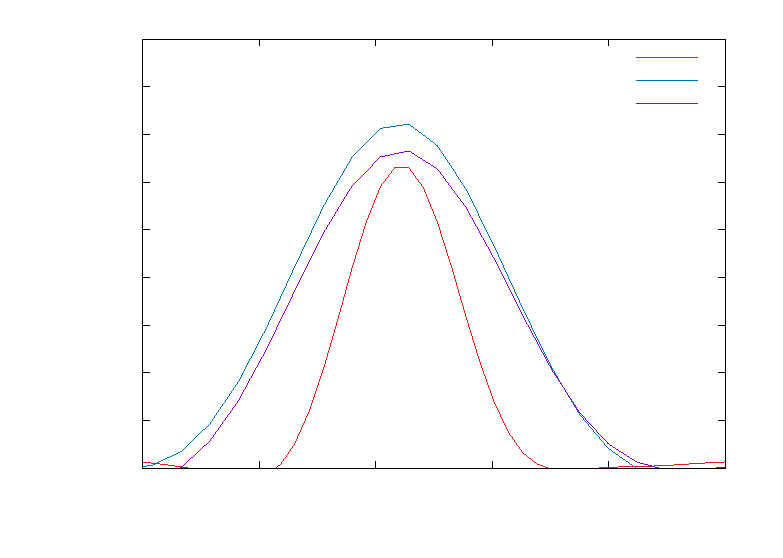
\includegraphics{plots/SignalkontrastT2}}%
    \gplfronttext
  \end{picture}%
\endgroup

    %     \caption{Die T2 Signale bei der jeweiligen Konzentration}
    % \end{figure}
    %  ich glaube die Abbildung ist nicht gut genug, 
    % bzw. die Fehlerdiskussion hätte ich keine Ahnung, warum 1000mol in der Mitte von den zwei ist


% !TEX root = main.tex
\section{T1 und T2 Relaxationszeit für Wasser und mit Zusatzmitteln}
\begin{figure}[H]
    \centering
    % GNUPLOT: LaTeX picture with Postscript
\begingroup
  % Encoding inside the plot.  In the header of your document, this encoding
  % should to defined, e.g., by using
  % \usepackage[cp1252,<other encodings>]{inputenc}
  \inputencoding{cp1252}%
  \makeatletter
  \providecommand\color[2][]{%
    \GenericError{(gnuplot) \space\space\space\@spaces}{%
      Package color not loaded in conjunction with
      terminal option `colourtext'%
    }{See the gnuplot documentation for explanation.%
    }{Either use 'blacktext' in gnuplot or load the package
      color.sty in LaTeX.}%
    \renewcommand\color[2][]{}%
  }%
  \providecommand\includegraphics[2][]{%
    \GenericError{(gnuplot) \space\space\space\@spaces}{%
      Package graphicx or graphics not loaded%
    }{See the gnuplot documentation for explanation.%
    }{The gnuplot epslatex terminal needs graphicx.sty or graphics.sty.}%
    \renewcommand\includegraphics[2][]{}%
  }%
  \providecommand\rotatebox[2]{#2}%
  \@ifundefined{ifGPcolor}{%
    \newif\ifGPcolor
    \GPcolorfalse
  }{}%
  \@ifundefined{ifGPblacktext}{%
    \newif\ifGPblacktext
    \GPblacktexttrue
  }{}%
  % define a \g@addto@macro without @ in the name:
  \let\gplgaddtomacro\g@addto@macro
  % define empty templates for all commands taking text:
  \gdef\gplbacktext{}%
  \gdef\gplfronttext{}%
  \makeatother
  \ifGPblacktext
    % no textcolor at all
    \def\colorrgb#1{}%
    \def\colorgray#1{}%
  \else
    % gray or color?
    \ifGPcolor
      \def\colorrgb#1{\color[rgb]{#1}}%
      \def\colorgray#1{\color[gray]{#1}}%
      \expandafter\def\csname LTw\endcsname{\color{white}}%
      \expandafter\def\csname LTb\endcsname{\color{black}}%
      \expandafter\def\csname LTa\endcsname{\color{black}}%
      \expandafter\def\csname LT0\endcsname{\color[rgb]{1,0,0}}%
      \expandafter\def\csname LT1\endcsname{\color[rgb]{0,1,0}}%
      \expandafter\def\csname LT2\endcsname{\color[rgb]{0,0,1}}%
      \expandafter\def\csname LT3\endcsname{\color[rgb]{1,0,1}}%
      \expandafter\def\csname LT4\endcsname{\color[rgb]{0,1,1}}%
      \expandafter\def\csname LT5\endcsname{\color[rgb]{1,1,0}}%
      \expandafter\def\csname LT6\endcsname{\color[rgb]{0,0,0}}%
      \expandafter\def\csname LT7\endcsname{\color[rgb]{1,0.3,0}}%
      \expandafter\def\csname LT8\endcsname{\color[rgb]{0.5,0.5,0.5}}%
    \else
      % gray
      \def\colorrgb#1{\color{black}}%
      \def\colorgray#1{\color[gray]{#1}}%
      \expandafter\def\csname LTw\endcsname{\color{white}}%
      \expandafter\def\csname LTb\endcsname{\color{black}}%
      \expandafter\def\csname LTa\endcsname{\color{black}}%
      \expandafter\def\csname LT0\endcsname{\color{black}}%
      \expandafter\def\csname LT1\endcsname{\color{black}}%
      \expandafter\def\csname LT2\endcsname{\color{black}}%
      \expandafter\def\csname LT3\endcsname{\color{black}}%
      \expandafter\def\csname LT4\endcsname{\color{black}}%
      \expandafter\def\csname LT5\endcsname{\color{black}}%
      \expandafter\def\csname LT6\endcsname{\color{black}}%
      \expandafter\def\csname LT7\endcsname{\color{black}}%
      \expandafter\def\csname LT8\endcsname{\color{black}}%
    \fi
  \fi
    \setlength{\unitlength}{0.0500bp}%
    \ifx\gptboxheight\undefined%
      \newlength{\gptboxheight}%
      \newlength{\gptboxwidth}%
      \newsavebox{\gptboxtext}%
    \fi%
    \setlength{\fboxrule}{0.5pt}%
    \setlength{\fboxsep}{1pt}%
\begin{picture}(7200.00,5040.00)%
    \gplgaddtomacro\gplbacktext{%
      \csname LTb\endcsname%%
      \put(814,704){\makebox(0,0)[r]{\strut{}$0$}}%
      \put(814,1527){\makebox(0,0)[r]{\strut{}$0.2$}}%
      \put(814,2350){\makebox(0,0)[r]{\strut{}$0.4$}}%
      \put(814,3173){\makebox(0,0)[r]{\strut{}$0.6$}}%
      \put(814,3996){\makebox(0,0)[r]{\strut{}$0.8$}}%
      \put(814,4819){\makebox(0,0)[r]{\strut{}$1$}}%
      \put(946,484){\makebox(0,0){\strut{}$0$}}%
      \put(1660,484){\makebox(0,0){\strut{}$500$}}%
      \put(2375,484){\makebox(0,0){\strut{}$1000$}}%
      \put(3089,484){\makebox(0,0){\strut{}$1500$}}%
      \put(3803,484){\makebox(0,0){\strut{}$2000$}}%
      \put(4517,484){\makebox(0,0){\strut{}$2500$}}%
      \put(5232,484){\makebox(0,0){\strut{}$3000$}}%
      \put(5946,484){\makebox(0,0){\strut{}$3500$}}%
      \put(6660,484){\makebox(0,0){\strut{}$4000$}}%
    }%
    \gplgaddtomacro\gplfronttext{%
      \csname LTb\endcsname%%
      \put(308,2761){\rotatebox{-270}{\makebox(0,0){\strut{}D\"ampfung $\frac{\text{E}}{\text{E}_0}$}}}%
      \put(3874,154){\makebox(0,0){\strut{}Zeit zwischen den Pulsen $t$ in $\si{\milli \second}$}}%
      \csname LTb\endcsname%%
      \put(5860,4606){\makebox(0,0)[r]{\strut{}gemessene Datenpunkte f\"ur Wasser}}%
      \csname LTb\endcsname%%
      \put(5860,4386){\makebox(0,0)[r]{\strut{}exponentieller Fit}}%
    }%
    \gplbacktext
    \put(0,0){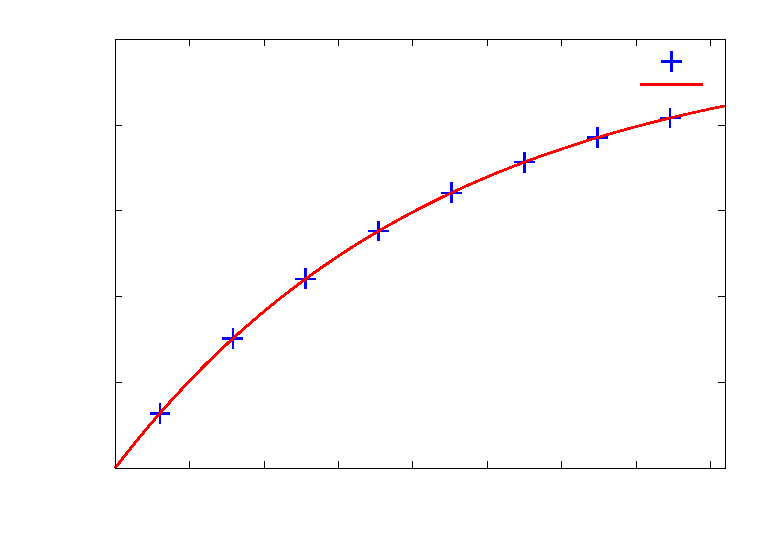
\includegraphics{plots/T1Wasser}}%
    \gplfronttext
  \end{picture}%
\endgroup

    \caption{T1 Messung von Wasser}
\end{figure}

\begin{figure}[H]
    \centering
    % GNUPLOT: LaTeX picture with Postscript
\begingroup
  % Encoding inside the plot.  In the header of your document, this encoding
  % should to defined, e.g., by using
  % \usepackage[cp1252,<other encodings>]{inputenc}
  \inputencoding{cp1252}%
  \makeatletter
  \providecommand\color[2][]{%
    \GenericError{(gnuplot) \space\space\space\@spaces}{%
      Package color not loaded in conjunction with
      terminal option `colourtext'%
    }{See the gnuplot documentation for explanation.%
    }{Either use 'blacktext' in gnuplot or load the package
      color.sty in LaTeX.}%
    \renewcommand\color[2][]{}%
  }%
  \providecommand\includegraphics[2][]{%
    \GenericError{(gnuplot) \space\space\space\@spaces}{%
      Package graphicx or graphics not loaded%
    }{See the gnuplot documentation for explanation.%
    }{The gnuplot epslatex terminal needs graphicx.sty or graphics.sty.}%
    \renewcommand\includegraphics[2][]{}%
  }%
  \providecommand\rotatebox[2]{#2}%
  \@ifundefined{ifGPcolor}{%
    \newif\ifGPcolor
    \GPcolorfalse
  }{}%
  \@ifundefined{ifGPblacktext}{%
    \newif\ifGPblacktext
    \GPblacktexttrue
  }{}%
  % define a \g@addto@macro without @ in the name:
  \let\gplgaddtomacro\g@addto@macro
  % define empty templates for all commands taking text:
  \gdef\gplbacktext{}%
  \gdef\gplfronttext{}%
  \makeatother
  \ifGPblacktext
    % no textcolor at all
    \def\colorrgb#1{}%
    \def\colorgray#1{}%
  \else
    % gray or color?
    \ifGPcolor
      \def\colorrgb#1{\color[rgb]{#1}}%
      \def\colorgray#1{\color[gray]{#1}}%
      \expandafter\def\csname LTw\endcsname{\color{white}}%
      \expandafter\def\csname LTb\endcsname{\color{black}}%
      \expandafter\def\csname LTa\endcsname{\color{black}}%
      \expandafter\def\csname LT0\endcsname{\color[rgb]{1,0,0}}%
      \expandafter\def\csname LT1\endcsname{\color[rgb]{0,1,0}}%
      \expandafter\def\csname LT2\endcsname{\color[rgb]{0,0,1}}%
      \expandafter\def\csname LT3\endcsname{\color[rgb]{1,0,1}}%
      \expandafter\def\csname LT4\endcsname{\color[rgb]{0,1,1}}%
      \expandafter\def\csname LT5\endcsname{\color[rgb]{1,1,0}}%
      \expandafter\def\csname LT6\endcsname{\color[rgb]{0,0,0}}%
      \expandafter\def\csname LT7\endcsname{\color[rgb]{1,0.3,0}}%
      \expandafter\def\csname LT8\endcsname{\color[rgb]{0.5,0.5,0.5}}%
    \else
      % gray
      \def\colorrgb#1{\color{black}}%
      \def\colorgray#1{\color[gray]{#1}}%
      \expandafter\def\csname LTw\endcsname{\color{white}}%
      \expandafter\def\csname LTb\endcsname{\color{black}}%
      \expandafter\def\csname LTa\endcsname{\color{black}}%
      \expandafter\def\csname LT0\endcsname{\color{black}}%
      \expandafter\def\csname LT1\endcsname{\color{black}}%
      \expandafter\def\csname LT2\endcsname{\color{black}}%
      \expandafter\def\csname LT3\endcsname{\color{black}}%
      \expandafter\def\csname LT4\endcsname{\color{black}}%
      \expandafter\def\csname LT5\endcsname{\color{black}}%
      \expandafter\def\csname LT6\endcsname{\color{black}}%
      \expandafter\def\csname LT7\endcsname{\color{black}}%
      \expandafter\def\csname LT8\endcsname{\color{black}}%
    \fi
  \fi
    \setlength{\unitlength}{0.0500bp}%
    \ifx\gptboxheight\undefined%
      \newlength{\gptboxheight}%
      \newlength{\gptboxwidth}%
      \newsavebox{\gptboxtext}%
    \fi%
    \setlength{\fboxrule}{0.5pt}%
    \setlength{\fboxsep}{1pt}%
\begin{picture}(7200.00,5040.00)%
    \gplgaddtomacro\gplbacktext{%
      \csname LTb\endcsname%%
      \put(814,704){\makebox(0,0)[r]{\strut{}$0$}}%
      \put(814,1527){\makebox(0,0)[r]{\strut{}$0.2$}}%
      \put(814,2350){\makebox(0,0)[r]{\strut{}$0.4$}}%
      \put(814,3173){\makebox(0,0)[r]{\strut{}$0.6$}}%
      \put(814,3996){\makebox(0,0)[r]{\strut{}$0.8$}}%
      \put(814,4819){\makebox(0,0)[r]{\strut{}$1$}}%
      \put(946,484){\makebox(0,0){\strut{}$0$}}%
      \put(1922,484){\makebox(0,0){\strut{}$1000$}}%
      \put(2898,484){\makebox(0,0){\strut{}$2000$}}%
      \put(3875,484){\makebox(0,0){\strut{}$3000$}}%
      \put(4851,484){\makebox(0,0){\strut{}$4000$}}%
      \put(5827,484){\makebox(0,0){\strut{}$5000$}}%
      \put(6803,484){\makebox(0,0){\strut{}$6000$}}%
    }%
    \gplgaddtomacro\gplfronttext{%
      \csname LTb\endcsname%%
      \put(308,2761){\rotatebox{-270}{\makebox(0,0){\strut{}Dämpfung $\frac{\text{E}}{\text{E}_0}$}}}%
      \put(3874,154){\makebox(0,0){\strut{}Zeit in $\si{\milli \second}$}}%
      \csname LTb\endcsname%%
      \put(5860,4606){\makebox(0,0)[r]{\strut{}gemessene Datenpunkte für Wasser}}%
      \csname LTb\endcsname%%
      \put(5860,4386){\makebox(0,0)[r]{\strut{}Dämpfungsfit Fit}}%
    }%
    \gplbacktext
    \put(0,0){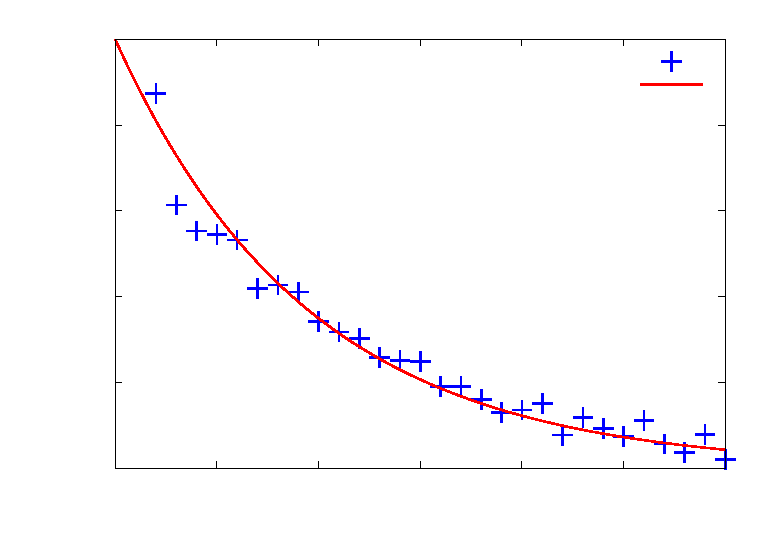
\includegraphics{plots/T2Wasser}}%
    \gplfronttext
  \end{picture}%
\endgroup

    \caption{T2 Messung von Wasser}
\end{figure}

% \begin{figure}[H]
%     \centering
%     % GNUPLOT: LaTeX picture with Postscript
\begingroup
  % Encoding inside the plot.  In the header of your document, this encoding
  % should to defined, e.g., by using
  % \usepackage[cp1252,<other encodings>]{inputenc}
  \inputencoding{cp1252}%
  \makeatletter
  \providecommand\color[2][]{%
    \GenericError{(gnuplot) \space\space\space\@spaces}{%
      Package color not loaded in conjunction with
      terminal option `colourtext'%
    }{See the gnuplot documentation for explanation.%
    }{Either use 'blacktext' in gnuplot or load the package
      color.sty in LaTeX.}%
    \renewcommand\color[2][]{}%
  }%
  \providecommand\includegraphics[2][]{%
    \GenericError{(gnuplot) \space\space\space\@spaces}{%
      Package graphicx or graphics not loaded%
    }{See the gnuplot documentation for explanation.%
    }{The gnuplot epslatex terminal needs graphicx.sty or graphics.sty.}%
    \renewcommand\includegraphics[2][]{}%
  }%
  \providecommand\rotatebox[2]{#2}%
  \@ifundefined{ifGPcolor}{%
    \newif\ifGPcolor
    \GPcolorfalse
  }{}%
  \@ifundefined{ifGPblacktext}{%
    \newif\ifGPblacktext
    \GPblacktexttrue
  }{}%
  % define a \g@addto@macro without @ in the name:
  \let\gplgaddtomacro\g@addto@macro
  % define empty templates for all commands taking text:
  \gdef\gplbacktext{}%
  \gdef\gplfronttext{}%
  \makeatother
  \ifGPblacktext
    % no textcolor at all
    \def\colorrgb#1{}%
    \def\colorgray#1{}%
  \else
    % gray or color?
    \ifGPcolor
      \def\colorrgb#1{\color[rgb]{#1}}%
      \def\colorgray#1{\color[gray]{#1}}%
      \expandafter\def\csname LTw\endcsname{\color{white}}%
      \expandafter\def\csname LTb\endcsname{\color{black}}%
      \expandafter\def\csname LTa\endcsname{\color{black}}%
      \expandafter\def\csname LT0\endcsname{\color[rgb]{1,0,0}}%
      \expandafter\def\csname LT1\endcsname{\color[rgb]{0,1,0}}%
      \expandafter\def\csname LT2\endcsname{\color[rgb]{0,0,1}}%
      \expandafter\def\csname LT3\endcsname{\color[rgb]{1,0,1}}%
      \expandafter\def\csname LT4\endcsname{\color[rgb]{0,1,1}}%
      \expandafter\def\csname LT5\endcsname{\color[rgb]{1,1,0}}%
      \expandafter\def\csname LT6\endcsname{\color[rgb]{0,0,0}}%
      \expandafter\def\csname LT7\endcsname{\color[rgb]{1,0.3,0}}%
      \expandafter\def\csname LT8\endcsname{\color[rgb]{0.5,0.5,0.5}}%
    \else
      % gray
      \def\colorrgb#1{\color{black}}%
      \def\colorgray#1{\color[gray]{#1}}%
      \expandafter\def\csname LTw\endcsname{\color{white}}%
      \expandafter\def\csname LTb\endcsname{\color{black}}%
      \expandafter\def\csname LTa\endcsname{\color{black}}%
      \expandafter\def\csname LT0\endcsname{\color{black}}%
      \expandafter\def\csname LT1\endcsname{\color{black}}%
      \expandafter\def\csname LT2\endcsname{\color{black}}%
      \expandafter\def\csname LT3\endcsname{\color{black}}%
      \expandafter\def\csname LT4\endcsname{\color{black}}%
      \expandafter\def\csname LT5\endcsname{\color{black}}%
      \expandafter\def\csname LT6\endcsname{\color{black}}%
      \expandafter\def\csname LT7\endcsname{\color{black}}%
      \expandafter\def\csname LT8\endcsname{\color{black}}%
    \fi
  \fi
    \setlength{\unitlength}{0.0500bp}%
    \ifx\gptboxheight\undefined%
      \newlength{\gptboxheight}%
      \newlength{\gptboxwidth}%
      \newsavebox{\gptboxtext}%
    \fi%
    \setlength{\fboxrule}{0.5pt}%
    \setlength{\fboxsep}{1pt}%
\begin{picture}(7200.00,5040.00)%
    \gplgaddtomacro\gplbacktext{%
      \csname LTb\endcsname%%
      \put(814,704){\makebox(0,0)[r]{\strut{}$0$}}%
      \put(814,1527){\makebox(0,0)[r]{\strut{}$0.2$}}%
      \put(814,2350){\makebox(0,0)[r]{\strut{}$0.4$}}%
      \put(814,3173){\makebox(0,0)[r]{\strut{}$0.6$}}%
      \put(814,3996){\makebox(0,0)[r]{\strut{}$0.8$}}%
      \put(814,4819){\makebox(0,0)[r]{\strut{}$1$}}%
      \put(946,484){\makebox(0,0){\strut{}$0$}}%
      \put(1563,484){\makebox(0,0){\strut{}$500$}}%
      \put(2179,484){\makebox(0,0){\strut{}$1000$}}%
      \put(2796,484){\makebox(0,0){\strut{}$1500$}}%
      \put(3412,484){\makebox(0,0){\strut{}$2000$}}%
      \put(4029,484){\makebox(0,0){\strut{}$2500$}}%
      \put(4645,484){\makebox(0,0){\strut{}$3000$}}%
      \put(5262,484){\makebox(0,0){\strut{}$3500$}}%
      \put(5878,484){\makebox(0,0){\strut{}$4000$}}%
      \put(6495,484){\makebox(0,0){\strut{}$4500$}}%
    }%
    \gplgaddtomacro\gplfronttext{%
      \csname LTb\endcsname%%
      \put(308,2761){\rotatebox{-270}{\makebox(0,0){\strut{}D\"ampfung $\frac{\text{E}}{\text{E}_0}$}}}%
      \put(3874,154){\makebox(0,0){\strut{}Zeit zwischen den Pulsen $t$ in $\si{\milli \second}$}}%
      \csname LTb\endcsname%%
      \put(5860,4606){\makebox(0,0)[r]{\strut{}gemessene Datenpunkte f\"ur $Cu^{2+} \SI{250}{\micro\mole}$}}%
      \csname LTb\endcsname%%
      \put(5860,4386){\makebox(0,0)[r]{\strut{}exponentieller Fit}}%
    }%
    \gplbacktext
    \put(0,0){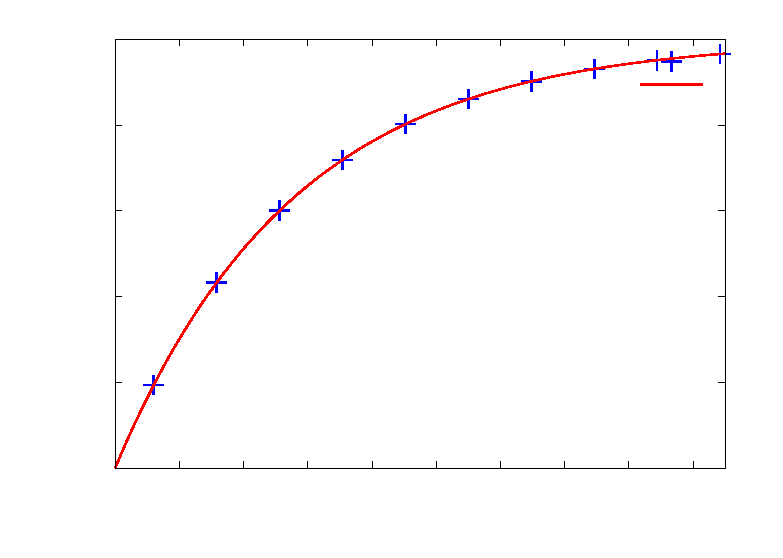
\includegraphics{plots/T1Kupfer250}}%
    \gplfronttext
  \end{picture}%
\endgroup

%     \caption{T1 Messung Kupfer $Cu^{2+} \SI{250}{\micro\mole}$}
% \end{figure}

% \begin{figure}[H]
%     \centering
%     % GNUPLOT: LaTeX picture with Postscript
\begingroup
  % Encoding inside the plot.  In the header of your document, this encoding
  % should to defined, e.g., by using
  % \usepackage[cp1252,<other encodings>]{inputenc}
  \inputencoding{cp1252}%
  \makeatletter
  \providecommand\color[2][]{%
    \GenericError{(gnuplot) \space\space\space\@spaces}{%
      Package color not loaded in conjunction with
      terminal option `colourtext'%
    }{See the gnuplot documentation for explanation.%
    }{Either use 'blacktext' in gnuplot or load the package
      color.sty in LaTeX.}%
    \renewcommand\color[2][]{}%
  }%
  \providecommand\includegraphics[2][]{%
    \GenericError{(gnuplot) \space\space\space\@spaces}{%
      Package graphicx or graphics not loaded%
    }{See the gnuplot documentation for explanation.%
    }{The gnuplot epslatex terminal needs graphicx.sty or graphics.sty.}%
    \renewcommand\includegraphics[2][]{}%
  }%
  \providecommand\rotatebox[2]{#2}%
  \@ifundefined{ifGPcolor}{%
    \newif\ifGPcolor
    \GPcolorfalse
  }{}%
  \@ifundefined{ifGPblacktext}{%
    \newif\ifGPblacktext
    \GPblacktexttrue
  }{}%
  % define a \g@addto@macro without @ in the name:
  \let\gplgaddtomacro\g@addto@macro
  % define empty templates for all commands taking text:
  \gdef\gplbacktext{}%
  \gdef\gplfronttext{}%
  \makeatother
  \ifGPblacktext
    % no textcolor at all
    \def\colorrgb#1{}%
    \def\colorgray#1{}%
  \else
    % gray or color?
    \ifGPcolor
      \def\colorrgb#1{\color[rgb]{#1}}%
      \def\colorgray#1{\color[gray]{#1}}%
      \expandafter\def\csname LTw\endcsname{\color{white}}%
      \expandafter\def\csname LTb\endcsname{\color{black}}%
      \expandafter\def\csname LTa\endcsname{\color{black}}%
      \expandafter\def\csname LT0\endcsname{\color[rgb]{1,0,0}}%
      \expandafter\def\csname LT1\endcsname{\color[rgb]{0,1,0}}%
      \expandafter\def\csname LT2\endcsname{\color[rgb]{0,0,1}}%
      \expandafter\def\csname LT3\endcsname{\color[rgb]{1,0,1}}%
      \expandafter\def\csname LT4\endcsname{\color[rgb]{0,1,1}}%
      \expandafter\def\csname LT5\endcsname{\color[rgb]{1,1,0}}%
      \expandafter\def\csname LT6\endcsname{\color[rgb]{0,0,0}}%
      \expandafter\def\csname LT7\endcsname{\color[rgb]{1,0.3,0}}%
      \expandafter\def\csname LT8\endcsname{\color[rgb]{0.5,0.5,0.5}}%
    \else
      % gray
      \def\colorrgb#1{\color{black}}%
      \def\colorgray#1{\color[gray]{#1}}%
      \expandafter\def\csname LTw\endcsname{\color{white}}%
      \expandafter\def\csname LTb\endcsname{\color{black}}%
      \expandafter\def\csname LTa\endcsname{\color{black}}%
      \expandafter\def\csname LT0\endcsname{\color{black}}%
      \expandafter\def\csname LT1\endcsname{\color{black}}%
      \expandafter\def\csname LT2\endcsname{\color{black}}%
      \expandafter\def\csname LT3\endcsname{\color{black}}%
      \expandafter\def\csname LT4\endcsname{\color{black}}%
      \expandafter\def\csname LT5\endcsname{\color{black}}%
      \expandafter\def\csname LT6\endcsname{\color{black}}%
      \expandafter\def\csname LT7\endcsname{\color{black}}%
      \expandafter\def\csname LT8\endcsname{\color{black}}%
    \fi
  \fi
    \setlength{\unitlength}{0.0500bp}%
    \ifx\gptboxheight\undefined%
      \newlength{\gptboxheight}%
      \newlength{\gptboxwidth}%
      \newsavebox{\gptboxtext}%
    \fi%
    \setlength{\fboxrule}{0.5pt}%
    \setlength{\fboxsep}{1pt}%
\begin{picture}(7200.00,5040.00)%
    \gplgaddtomacro\gplbacktext{%
      \csname LTb\endcsname%%
      \put(814,704){\makebox(0,0)[r]{\strut{}$0$}}%
      \put(814,1527){\makebox(0,0)[r]{\strut{}$0.2$}}%
      \put(814,2350){\makebox(0,0)[r]{\strut{}$0.4$}}%
      \put(814,3173){\makebox(0,0)[r]{\strut{}$0.6$}}%
      \put(814,3996){\makebox(0,0)[r]{\strut{}$0.8$}}%
      \put(814,4819){\makebox(0,0)[r]{\strut{}$1$}}%
      \put(946,484){\makebox(0,0){\strut{}$0$}}%
      \put(1922,484){\makebox(0,0){\strut{}$1000$}}%
      \put(2898,484){\makebox(0,0){\strut{}$2000$}}%
      \put(3875,484){\makebox(0,0){\strut{}$3000$}}%
      \put(4851,484){\makebox(0,0){\strut{}$4000$}}%
      \put(5827,484){\makebox(0,0){\strut{}$5000$}}%
      \put(6803,484){\makebox(0,0){\strut{}$6000$}}%
    }%
    \gplgaddtomacro\gplfronttext{%
      \csname LTb\endcsname%%
      \put(308,2761){\rotatebox{-270}{\makebox(0,0){\strut{}Dämpfung $\frac{\text{E}}{\text{E}_0}$}}}%
      \put(3874,154){\makebox(0,0){\strut{}Zeit in $\si{\milli \second}$}}%
      \csname LTb\endcsname%%
      \put(5816,4646){\makebox(0,0)[r]{\strut{}gemessene Datenpunkte für $Cu^{2+} \SI{250}{\micro\mole}$}}%
      \csname LTb\endcsname%%
      \put(5816,4426){\makebox(0,0)[r]{\strut{}Dämpfungsfit Fit}}%
    }%
    \gplbacktext
    \put(0,0){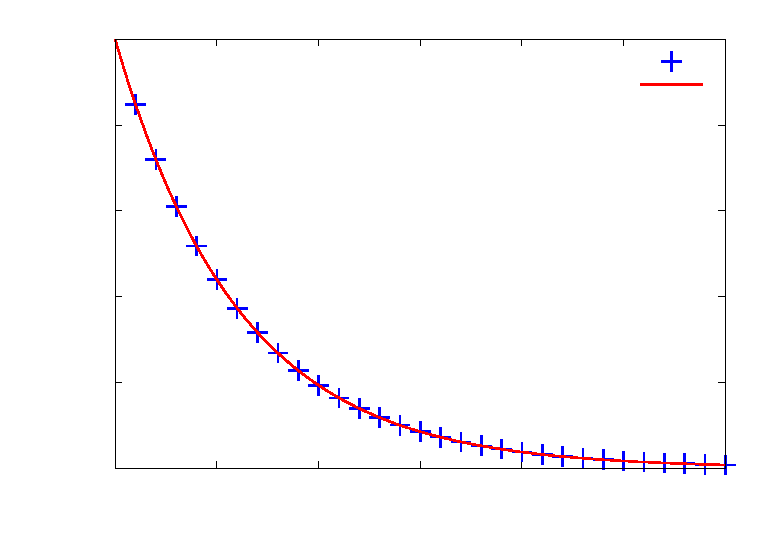
\includegraphics{plots/T2Kupfer250}}%
    \gplfronttext
  \end{picture}%
\endgroup

%     \caption{T2 Messung Kupfer $Cu^{2+} \SI{250}{\micro\mole}$}
% \end{figure}
% \begin{figure}[H]
%     \centering
%     % GNUPLOT: LaTeX picture with Postscript
\begingroup
  % Encoding inside the plot.  In the header of your document, this encoding
  % should to defined, e.g., by using
  % \usepackage[cp1252,<other encodings>]{inputenc}
  \inputencoding{cp1252}%
  \makeatletter
  \providecommand\color[2][]{%
    \GenericError{(gnuplot) \space\space\space\@spaces}{%
      Package color not loaded in conjunction with
      terminal option `colourtext'%
    }{See the gnuplot documentation for explanation.%
    }{Either use 'blacktext' in gnuplot or load the package
      color.sty in LaTeX.}%
    \renewcommand\color[2][]{}%
  }%
  \providecommand\includegraphics[2][]{%
    \GenericError{(gnuplot) \space\space\space\@spaces}{%
      Package graphicx or graphics not loaded%
    }{See the gnuplot documentation for explanation.%
    }{The gnuplot epslatex terminal needs graphicx.sty or graphics.sty.}%
    \renewcommand\includegraphics[2][]{}%
  }%
  \providecommand\rotatebox[2]{#2}%
  \@ifundefined{ifGPcolor}{%
    \newif\ifGPcolor
    \GPcolorfalse
  }{}%
  \@ifundefined{ifGPblacktext}{%
    \newif\ifGPblacktext
    \GPblacktexttrue
  }{}%
  % define a \g@addto@macro without @ in the name:
  \let\gplgaddtomacro\g@addto@macro
  % define empty templates for all commands taking text:
  \gdef\gplbacktext{}%
  \gdef\gplfronttext{}%
  \makeatother
  \ifGPblacktext
    % no textcolor at all
    \def\colorrgb#1{}%
    \def\colorgray#1{}%
  \else
    % gray or color?
    \ifGPcolor
      \def\colorrgb#1{\color[rgb]{#1}}%
      \def\colorgray#1{\color[gray]{#1}}%
      \expandafter\def\csname LTw\endcsname{\color{white}}%
      \expandafter\def\csname LTb\endcsname{\color{black}}%
      \expandafter\def\csname LTa\endcsname{\color{black}}%
      \expandafter\def\csname LT0\endcsname{\color[rgb]{1,0,0}}%
      \expandafter\def\csname LT1\endcsname{\color[rgb]{0,1,0}}%
      \expandafter\def\csname LT2\endcsname{\color[rgb]{0,0,1}}%
      \expandafter\def\csname LT3\endcsname{\color[rgb]{1,0,1}}%
      \expandafter\def\csname LT4\endcsname{\color[rgb]{0,1,1}}%
      \expandafter\def\csname LT5\endcsname{\color[rgb]{1,1,0}}%
      \expandafter\def\csname LT6\endcsname{\color[rgb]{0,0,0}}%
      \expandafter\def\csname LT7\endcsname{\color[rgb]{1,0.3,0}}%
      \expandafter\def\csname LT8\endcsname{\color[rgb]{0.5,0.5,0.5}}%
    \else
      % gray
      \def\colorrgb#1{\color{black}}%
      \def\colorgray#1{\color[gray]{#1}}%
      \expandafter\def\csname LTw\endcsname{\color{white}}%
      \expandafter\def\csname LTb\endcsname{\color{black}}%
      \expandafter\def\csname LTa\endcsname{\color{black}}%
      \expandafter\def\csname LT0\endcsname{\color{black}}%
      \expandafter\def\csname LT1\endcsname{\color{black}}%
      \expandafter\def\csname LT2\endcsname{\color{black}}%
      \expandafter\def\csname LT3\endcsname{\color{black}}%
      \expandafter\def\csname LT4\endcsname{\color{black}}%
      \expandafter\def\csname LT5\endcsname{\color{black}}%
      \expandafter\def\csname LT6\endcsname{\color{black}}%
      \expandafter\def\csname LT7\endcsname{\color{black}}%
      \expandafter\def\csname LT8\endcsname{\color{black}}%
    \fi
  \fi
    \setlength{\unitlength}{0.0500bp}%
    \ifx\gptboxheight\undefined%
      \newlength{\gptboxheight}%
      \newlength{\gptboxwidth}%
      \newsavebox{\gptboxtext}%
    \fi%
    \setlength{\fboxrule}{0.5pt}%
    \setlength{\fboxsep}{1pt}%
\begin{picture}(7200.00,5040.00)%
    \gplgaddtomacro\gplbacktext{%
      \csname LTb\endcsname%%
      \put(814,704){\makebox(0,0)[r]{\strut{}$0$}}%
      \put(814,1527){\makebox(0,0)[r]{\strut{}$0.2$}}%
      \put(814,2350){\makebox(0,0)[r]{\strut{}$0.4$}}%
      \put(814,3173){\makebox(0,0)[r]{\strut{}$0.6$}}%
      \put(814,3996){\makebox(0,0)[r]{\strut{}$0.8$}}%
      \put(814,4819){\makebox(0,0)[r]{\strut{}$1$}}%
      \put(946,484){\makebox(0,0){\strut{}$0$}}%
      \put(1563,484){\makebox(0,0){\strut{}$500$}}%
      \put(2179,484){\makebox(0,0){\strut{}$1000$}}%
      \put(2796,484){\makebox(0,0){\strut{}$1500$}}%
      \put(3412,484){\makebox(0,0){\strut{}$2000$}}%
      \put(4029,484){\makebox(0,0){\strut{}$2500$}}%
      \put(4645,484){\makebox(0,0){\strut{}$3000$}}%
      \put(5262,484){\makebox(0,0){\strut{}$3500$}}%
      \put(5878,484){\makebox(0,0){\strut{}$4000$}}%
      \put(6495,484){\makebox(0,0){\strut{}$4500$}}%
    }%
    \gplgaddtomacro\gplfronttext{%
      \csname LTb\endcsname%%
      \put(308,2761){\rotatebox{-270}{\makebox(0,0){\strut{}D\"ampfung $\frac{\text{E}}{\text{E}_0}$}}}%
      \put(3874,154){\makebox(0,0){\strut{}Zeit zwischen den Pulsen $t$ in $\si{\milli \second}$}}%
      \csname LTb\endcsname%%
      \put(5860,4606){\makebox(0,0)[r]{\strut{}gemessene Datenpunkte f\"ur $Cu^{2+} \SI{250}{\micro\mole}$}}%
      \csname LTb\endcsname%%
      \put(5860,4386){\makebox(0,0)[r]{\strut{}exponentieller Fit}}%
    }%
    \gplbacktext
    \put(0,0){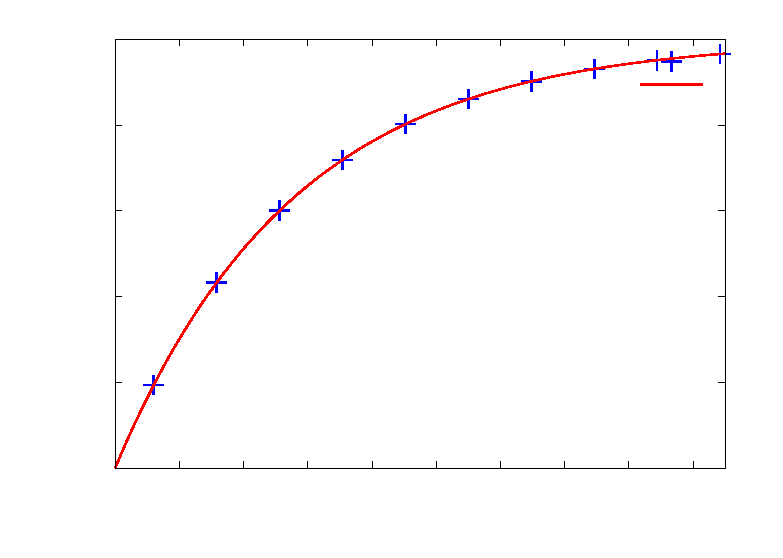
\includegraphics{plots/T1Kupfer250}}%
    \gplfronttext
  \end{picture}%
\endgroup

%     \caption{T1 Messung Kupfer $Cu^{2+} \SI{500}{\micro\mole}$}
% \end{figure}

% \begin{figure}[H]
%     \centering
%     % GNUPLOT: LaTeX picture with Postscript
\begingroup
  % Encoding inside the plot.  In the header of your document, this encoding
  % should to defined, e.g., by using
  % \usepackage[cp1252,<other encodings>]{inputenc}
  \inputencoding{cp1252}%
  \makeatletter
  \providecommand\color[2][]{%
    \GenericError{(gnuplot) \space\space\space\@spaces}{%
      Package color not loaded in conjunction with
      terminal option `colourtext'%
    }{See the gnuplot documentation for explanation.%
    }{Either use 'blacktext' in gnuplot or load the package
      color.sty in LaTeX.}%
    \renewcommand\color[2][]{}%
  }%
  \providecommand\includegraphics[2][]{%
    \GenericError{(gnuplot) \space\space\space\@spaces}{%
      Package graphicx or graphics not loaded%
    }{See the gnuplot documentation for explanation.%
    }{The gnuplot epslatex terminal needs graphicx.sty or graphics.sty.}%
    \renewcommand\includegraphics[2][]{}%
  }%
  \providecommand\rotatebox[2]{#2}%
  \@ifundefined{ifGPcolor}{%
    \newif\ifGPcolor
    \GPcolorfalse
  }{}%
  \@ifundefined{ifGPblacktext}{%
    \newif\ifGPblacktext
    \GPblacktexttrue
  }{}%
  % define a \g@addto@macro without @ in the name:
  \let\gplgaddtomacro\g@addto@macro
  % define empty templates for all commands taking text:
  \gdef\gplbacktext{}%
  \gdef\gplfronttext{}%
  \makeatother
  \ifGPblacktext
    % no textcolor at all
    \def\colorrgb#1{}%
    \def\colorgray#1{}%
  \else
    % gray or color?
    \ifGPcolor
      \def\colorrgb#1{\color[rgb]{#1}}%
      \def\colorgray#1{\color[gray]{#1}}%
      \expandafter\def\csname LTw\endcsname{\color{white}}%
      \expandafter\def\csname LTb\endcsname{\color{black}}%
      \expandafter\def\csname LTa\endcsname{\color{black}}%
      \expandafter\def\csname LT0\endcsname{\color[rgb]{1,0,0}}%
      \expandafter\def\csname LT1\endcsname{\color[rgb]{0,1,0}}%
      \expandafter\def\csname LT2\endcsname{\color[rgb]{0,0,1}}%
      \expandafter\def\csname LT3\endcsname{\color[rgb]{1,0,1}}%
      \expandafter\def\csname LT4\endcsname{\color[rgb]{0,1,1}}%
      \expandafter\def\csname LT5\endcsname{\color[rgb]{1,1,0}}%
      \expandafter\def\csname LT6\endcsname{\color[rgb]{0,0,0}}%
      \expandafter\def\csname LT7\endcsname{\color[rgb]{1,0.3,0}}%
      \expandafter\def\csname LT8\endcsname{\color[rgb]{0.5,0.5,0.5}}%
    \else
      % gray
      \def\colorrgb#1{\color{black}}%
      \def\colorgray#1{\color[gray]{#1}}%
      \expandafter\def\csname LTw\endcsname{\color{white}}%
      \expandafter\def\csname LTb\endcsname{\color{black}}%
      \expandafter\def\csname LTa\endcsname{\color{black}}%
      \expandafter\def\csname LT0\endcsname{\color{black}}%
      \expandafter\def\csname LT1\endcsname{\color{black}}%
      \expandafter\def\csname LT2\endcsname{\color{black}}%
      \expandafter\def\csname LT3\endcsname{\color{black}}%
      \expandafter\def\csname LT4\endcsname{\color{black}}%
      \expandafter\def\csname LT5\endcsname{\color{black}}%
      \expandafter\def\csname LT6\endcsname{\color{black}}%
      \expandafter\def\csname LT7\endcsname{\color{black}}%
      \expandafter\def\csname LT8\endcsname{\color{black}}%
    \fi
  \fi
    \setlength{\unitlength}{0.0500bp}%
    \ifx\gptboxheight\undefined%
      \newlength{\gptboxheight}%
      \newlength{\gptboxwidth}%
      \newsavebox{\gptboxtext}%
    \fi%
    \setlength{\fboxrule}{0.5pt}%
    \setlength{\fboxsep}{1pt}%
\begin{picture}(7200.00,5040.00)%
    \gplgaddtomacro\gplbacktext{%
      \csname LTb\endcsname%%
      \put(814,704){\makebox(0,0)[r]{\strut{}$0$}}%
      \put(814,1527){\makebox(0,0)[r]{\strut{}$0.2$}}%
      \put(814,2350){\makebox(0,0)[r]{\strut{}$0.4$}}%
      \put(814,3173){\makebox(0,0)[r]{\strut{}$0.6$}}%
      \put(814,3996){\makebox(0,0)[r]{\strut{}$0.8$}}%
      \put(814,4819){\makebox(0,0)[r]{\strut{}$1$}}%
      \put(946,484){\makebox(0,0){\strut{}$0$}}%
      \put(1922,484){\makebox(0,0){\strut{}$1000$}}%
      \put(2898,484){\makebox(0,0){\strut{}$2000$}}%
      \put(3875,484){\makebox(0,0){\strut{}$3000$}}%
      \put(4851,484){\makebox(0,0){\strut{}$4000$}}%
      \put(5827,484){\makebox(0,0){\strut{}$5000$}}%
      \put(6803,484){\makebox(0,0){\strut{}$6000$}}%
    }%
    \gplgaddtomacro\gplfronttext{%
      \csname LTb\endcsname%%
      \put(308,2761){\rotatebox{-270}{\makebox(0,0){\strut{}Dämpfung $\frac{\text{E}}{\text{E}_0}$}}}%
      \put(3874,154){\makebox(0,0){\strut{}Zeit in $\si{\milli \second}$}}%
      \csname LTb\endcsname%%
      \put(5816,4646){\makebox(0,0)[r]{\strut{}gemessene Datenpunkte für $Cu^{2+} \SI{250}{\micro\mole}$}}%
      \csname LTb\endcsname%%
      \put(5816,4426){\makebox(0,0)[r]{\strut{}Dämpfungsfit Fit}}%
    }%
    \gplbacktext
    \put(0,0){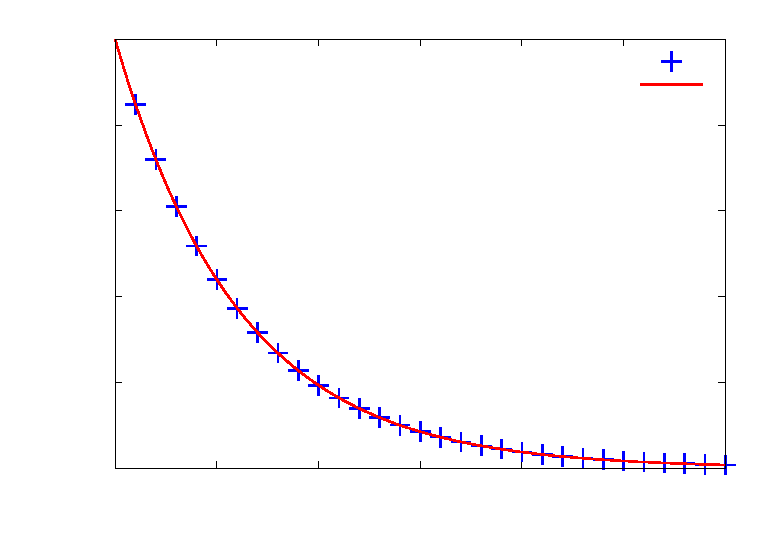
\includegraphics{plots/T2Kupfer250}}%
    \gplfronttext
  \end{picture}%
\endgroup

%     \caption{T2 Messung Kupfer $Cu^{2+} \SI{500}{\micro\mole}$}
% \end{figure}
% \begin{figure}[H]
%     \centering
%     % GNUPLOT: LaTeX picture with Postscript
\begingroup
  % Encoding inside the plot.  In the header of your document, this encoding
  % should to defined, e.g., by using
  % \usepackage[cp1252,<other encodings>]{inputenc}
  \inputencoding{cp1252}%
  \makeatletter
  \providecommand\color[2][]{%
    \GenericError{(gnuplot) \space\space\space\@spaces}{%
      Package color not loaded in conjunction with
      terminal option `colourtext'%
    }{See the gnuplot documentation for explanation.%
    }{Either use 'blacktext' in gnuplot or load the package
      color.sty in LaTeX.}%
    \renewcommand\color[2][]{}%
  }%
  \providecommand\includegraphics[2][]{%
    \GenericError{(gnuplot) \space\space\space\@spaces}{%
      Package graphicx or graphics not loaded%
    }{See the gnuplot documentation for explanation.%
    }{The gnuplot epslatex terminal needs graphicx.sty or graphics.sty.}%
    \renewcommand\includegraphics[2][]{}%
  }%
  \providecommand\rotatebox[2]{#2}%
  \@ifundefined{ifGPcolor}{%
    \newif\ifGPcolor
    \GPcolorfalse
  }{}%
  \@ifundefined{ifGPblacktext}{%
    \newif\ifGPblacktext
    \GPblacktexttrue
  }{}%
  % define a \g@addto@macro without @ in the name:
  \let\gplgaddtomacro\g@addto@macro
  % define empty templates for all commands taking text:
  \gdef\gplbacktext{}%
  \gdef\gplfronttext{}%
  \makeatother
  \ifGPblacktext
    % no textcolor at all
    \def\colorrgb#1{}%
    \def\colorgray#1{}%
  \else
    % gray or color?
    \ifGPcolor
      \def\colorrgb#1{\color[rgb]{#1}}%
      \def\colorgray#1{\color[gray]{#1}}%
      \expandafter\def\csname LTw\endcsname{\color{white}}%
      \expandafter\def\csname LTb\endcsname{\color{black}}%
      \expandafter\def\csname LTa\endcsname{\color{black}}%
      \expandafter\def\csname LT0\endcsname{\color[rgb]{1,0,0}}%
      \expandafter\def\csname LT1\endcsname{\color[rgb]{0,1,0}}%
      \expandafter\def\csname LT2\endcsname{\color[rgb]{0,0,1}}%
      \expandafter\def\csname LT3\endcsname{\color[rgb]{1,0,1}}%
      \expandafter\def\csname LT4\endcsname{\color[rgb]{0,1,1}}%
      \expandafter\def\csname LT5\endcsname{\color[rgb]{1,1,0}}%
      \expandafter\def\csname LT6\endcsname{\color[rgb]{0,0,0}}%
      \expandafter\def\csname LT7\endcsname{\color[rgb]{1,0.3,0}}%
      \expandafter\def\csname LT8\endcsname{\color[rgb]{0.5,0.5,0.5}}%
    \else
      % gray
      \def\colorrgb#1{\color{black}}%
      \def\colorgray#1{\color[gray]{#1}}%
      \expandafter\def\csname LTw\endcsname{\color{white}}%
      \expandafter\def\csname LTb\endcsname{\color{black}}%
      \expandafter\def\csname LTa\endcsname{\color{black}}%
      \expandafter\def\csname LT0\endcsname{\color{black}}%
      \expandafter\def\csname LT1\endcsname{\color{black}}%
      \expandafter\def\csname LT2\endcsname{\color{black}}%
      \expandafter\def\csname LT3\endcsname{\color{black}}%
      \expandafter\def\csname LT4\endcsname{\color{black}}%
      \expandafter\def\csname LT5\endcsname{\color{black}}%
      \expandafter\def\csname LT6\endcsname{\color{black}}%
      \expandafter\def\csname LT7\endcsname{\color{black}}%
      \expandafter\def\csname LT8\endcsname{\color{black}}%
    \fi
  \fi
    \setlength{\unitlength}{0.0500bp}%
    \ifx\gptboxheight\undefined%
      \newlength{\gptboxheight}%
      \newlength{\gptboxwidth}%
      \newsavebox{\gptboxtext}%
    \fi%
    \setlength{\fboxrule}{0.5pt}%
    \setlength{\fboxsep}{1pt}%
\begin{picture}(7200.00,5040.00)%
    \gplgaddtomacro\gplbacktext{%
      \csname LTb\endcsname%%
      \put(814,704){\makebox(0,0)[r]{\strut{}$0$}}%
      \put(814,1527){\makebox(0,0)[r]{\strut{}$0.2$}}%
      \put(814,2350){\makebox(0,0)[r]{\strut{}$0.4$}}%
      \put(814,3173){\makebox(0,0)[r]{\strut{}$0.6$}}%
      \put(814,3996){\makebox(0,0)[r]{\strut{}$0.8$}}%
      \put(814,4819){\makebox(0,0)[r]{\strut{}$1$}}%
      \put(946,484){\makebox(0,0){\strut{}$0$}}%
      \put(1563,484){\makebox(0,0){\strut{}$500$}}%
      \put(2179,484){\makebox(0,0){\strut{}$1000$}}%
      \put(2796,484){\makebox(0,0){\strut{}$1500$}}%
      \put(3412,484){\makebox(0,0){\strut{}$2000$}}%
      \put(4029,484){\makebox(0,0){\strut{}$2500$}}%
      \put(4645,484){\makebox(0,0){\strut{}$3000$}}%
      \put(5262,484){\makebox(0,0){\strut{}$3500$}}%
      \put(5878,484){\makebox(0,0){\strut{}$4000$}}%
      \put(6495,484){\makebox(0,0){\strut{}$4500$}}%
    }%
    \gplgaddtomacro\gplfronttext{%
      \csname LTb\endcsname%%
      \put(308,2761){\rotatebox{-270}{\makebox(0,0){\strut{}D\"ampfung $\frac{\text{E}}{\text{E}_0}$}}}%
      \put(3874,154){\makebox(0,0){\strut{}Zeit zwischen den Pulsen $t$ in $\si{\milli \second}$}}%
      \csname LTb\endcsname%%
      \put(5860,4606){\makebox(0,0)[r]{\strut{}gemessene Datenpunkte f\"ur $Cu^{2+} \SI{250}{\micro\mole}$}}%
      \csname LTb\endcsname%%
      \put(5860,4386){\makebox(0,0)[r]{\strut{}exponentieller Fit}}%
    }%
    \gplbacktext
    \put(0,0){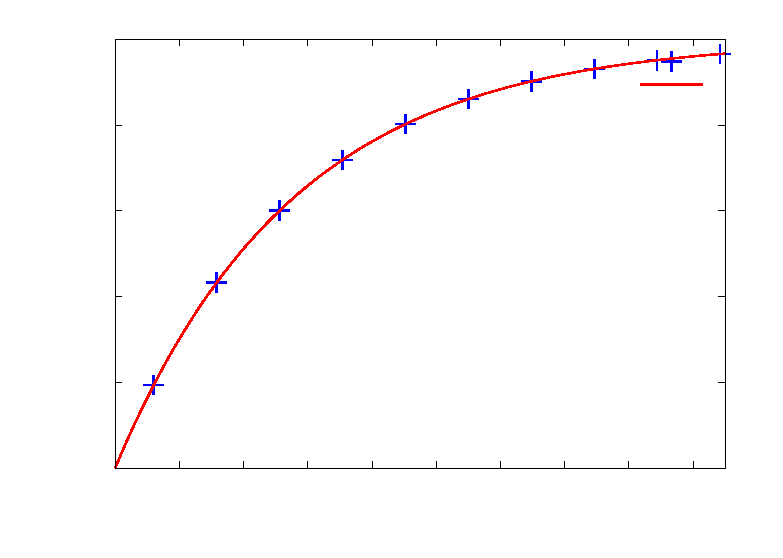
\includegraphics{plots/T1Kupfer250}}%
    \gplfronttext
  \end{picture}%
\endgroup

%     \caption{T1 Messung Kupfer $Cu^{2+} \SI{1000}{\micro\mole}$}
% \end{figure}

% \begin{figure}[H]
%     \centering
%     % GNUPLOT: LaTeX picture with Postscript
\begingroup
  % Encoding inside the plot.  In the header of your document, this encoding
  % should to defined, e.g., by using
  % \usepackage[cp1252,<other encodings>]{inputenc}
  \inputencoding{cp1252}%
  \makeatletter
  \providecommand\color[2][]{%
    \GenericError{(gnuplot) \space\space\space\@spaces}{%
      Package color not loaded in conjunction with
      terminal option `colourtext'%
    }{See the gnuplot documentation for explanation.%
    }{Either use 'blacktext' in gnuplot or load the package
      color.sty in LaTeX.}%
    \renewcommand\color[2][]{}%
  }%
  \providecommand\includegraphics[2][]{%
    \GenericError{(gnuplot) \space\space\space\@spaces}{%
      Package graphicx or graphics not loaded%
    }{See the gnuplot documentation for explanation.%
    }{The gnuplot epslatex terminal needs graphicx.sty or graphics.sty.}%
    \renewcommand\includegraphics[2][]{}%
  }%
  \providecommand\rotatebox[2]{#2}%
  \@ifundefined{ifGPcolor}{%
    \newif\ifGPcolor
    \GPcolorfalse
  }{}%
  \@ifundefined{ifGPblacktext}{%
    \newif\ifGPblacktext
    \GPblacktexttrue
  }{}%
  % define a \g@addto@macro without @ in the name:
  \let\gplgaddtomacro\g@addto@macro
  % define empty templates for all commands taking text:
  \gdef\gplbacktext{}%
  \gdef\gplfronttext{}%
  \makeatother
  \ifGPblacktext
    % no textcolor at all
    \def\colorrgb#1{}%
    \def\colorgray#1{}%
  \else
    % gray or color?
    \ifGPcolor
      \def\colorrgb#1{\color[rgb]{#1}}%
      \def\colorgray#1{\color[gray]{#1}}%
      \expandafter\def\csname LTw\endcsname{\color{white}}%
      \expandafter\def\csname LTb\endcsname{\color{black}}%
      \expandafter\def\csname LTa\endcsname{\color{black}}%
      \expandafter\def\csname LT0\endcsname{\color[rgb]{1,0,0}}%
      \expandafter\def\csname LT1\endcsname{\color[rgb]{0,1,0}}%
      \expandafter\def\csname LT2\endcsname{\color[rgb]{0,0,1}}%
      \expandafter\def\csname LT3\endcsname{\color[rgb]{1,0,1}}%
      \expandafter\def\csname LT4\endcsname{\color[rgb]{0,1,1}}%
      \expandafter\def\csname LT5\endcsname{\color[rgb]{1,1,0}}%
      \expandafter\def\csname LT6\endcsname{\color[rgb]{0,0,0}}%
      \expandafter\def\csname LT7\endcsname{\color[rgb]{1,0.3,0}}%
      \expandafter\def\csname LT8\endcsname{\color[rgb]{0.5,0.5,0.5}}%
    \else
      % gray
      \def\colorrgb#1{\color{black}}%
      \def\colorgray#1{\color[gray]{#1}}%
      \expandafter\def\csname LTw\endcsname{\color{white}}%
      \expandafter\def\csname LTb\endcsname{\color{black}}%
      \expandafter\def\csname LTa\endcsname{\color{black}}%
      \expandafter\def\csname LT0\endcsname{\color{black}}%
      \expandafter\def\csname LT1\endcsname{\color{black}}%
      \expandafter\def\csname LT2\endcsname{\color{black}}%
      \expandafter\def\csname LT3\endcsname{\color{black}}%
      \expandafter\def\csname LT4\endcsname{\color{black}}%
      \expandafter\def\csname LT5\endcsname{\color{black}}%
      \expandafter\def\csname LT6\endcsname{\color{black}}%
      \expandafter\def\csname LT7\endcsname{\color{black}}%
      \expandafter\def\csname LT8\endcsname{\color{black}}%
    \fi
  \fi
    \setlength{\unitlength}{0.0500bp}%
    \ifx\gptboxheight\undefined%
      \newlength{\gptboxheight}%
      \newlength{\gptboxwidth}%
      \newsavebox{\gptboxtext}%
    \fi%
    \setlength{\fboxrule}{0.5pt}%
    \setlength{\fboxsep}{1pt}%
\begin{picture}(7200.00,5040.00)%
    \gplgaddtomacro\gplbacktext{%
      \csname LTb\endcsname%%
      \put(814,704){\makebox(0,0)[r]{\strut{}$0$}}%
      \put(814,1527){\makebox(0,0)[r]{\strut{}$0.2$}}%
      \put(814,2350){\makebox(0,0)[r]{\strut{}$0.4$}}%
      \put(814,3173){\makebox(0,0)[r]{\strut{}$0.6$}}%
      \put(814,3996){\makebox(0,0)[r]{\strut{}$0.8$}}%
      \put(814,4819){\makebox(0,0)[r]{\strut{}$1$}}%
      \put(946,484){\makebox(0,0){\strut{}$0$}}%
      \put(1922,484){\makebox(0,0){\strut{}$1000$}}%
      \put(2898,484){\makebox(0,0){\strut{}$2000$}}%
      \put(3875,484){\makebox(0,0){\strut{}$3000$}}%
      \put(4851,484){\makebox(0,0){\strut{}$4000$}}%
      \put(5827,484){\makebox(0,0){\strut{}$5000$}}%
      \put(6803,484){\makebox(0,0){\strut{}$6000$}}%
    }%
    \gplgaddtomacro\gplfronttext{%
      \csname LTb\endcsname%%
      \put(308,2761){\rotatebox{-270}{\makebox(0,0){\strut{}Dämpfung $\frac{\text{E}}{\text{E}_0}$}}}%
      \put(3874,154){\makebox(0,0){\strut{}Zeit in $\si{\milli \second}$}}%
      \csname LTb\endcsname%%
      \put(5816,4646){\makebox(0,0)[r]{\strut{}gemessene Datenpunkte für $Cu^{2+} \SI{250}{\micro\mole}$}}%
      \csname LTb\endcsname%%
      \put(5816,4426){\makebox(0,0)[r]{\strut{}Dämpfungsfit Fit}}%
    }%
    \gplbacktext
    \put(0,0){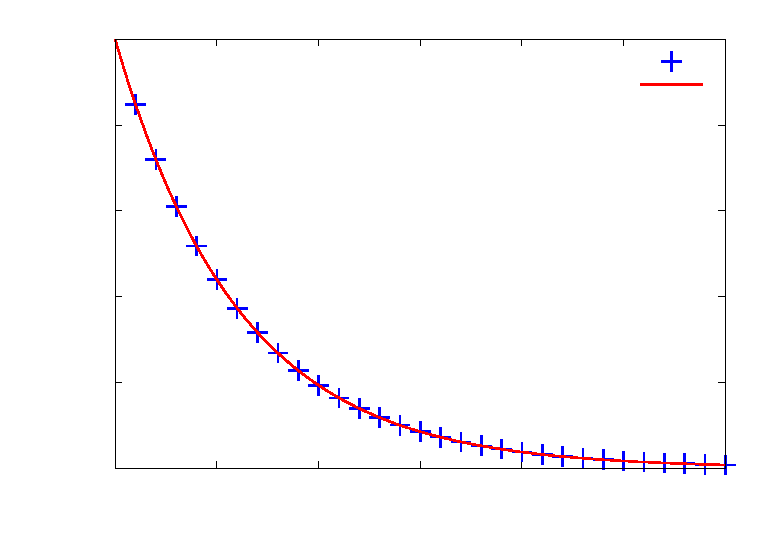
\includegraphics{plots/T2Kupfer250}}%
    \gplfronttext
  \end{picture}%
\endgroup

%     \caption{T2 Messung Kupfer $Cu^{2+} \SI{1000}{\micro\mole}$}
% \end{figure}

\begin{figure}[H]
    \centering
    % GNUPLOT: LaTeX picture with Postscript
\begingroup
  % Encoding inside the plot.  In the header of your document, this encoding
  % should to defined, e.g., by using
  % \usepackage[cp1252,<other encodings>]{inputenc}
  \inputencoding{cp1252}%
  \makeatletter
  \providecommand\color[2][]{%
    \GenericError{(gnuplot) \space\space\space\@spaces}{%
      Package color not loaded in conjunction with
      terminal option `colourtext'%
    }{See the gnuplot documentation for explanation.%
    }{Either use 'blacktext' in gnuplot or load the package
      color.sty in LaTeX.}%
    \renewcommand\color[2][]{}%
  }%
  \providecommand\includegraphics[2][]{%
    \GenericError{(gnuplot) \space\space\space\@spaces}{%
      Package graphicx or graphics not loaded%
    }{See the gnuplot documentation for explanation.%
    }{The gnuplot epslatex terminal needs graphicx.sty or graphics.sty.}%
    \renewcommand\includegraphics[2][]{}%
  }%
  \providecommand\rotatebox[2]{#2}%
  \@ifundefined{ifGPcolor}{%
    \newif\ifGPcolor
    \GPcolorfalse
  }{}%
  \@ifundefined{ifGPblacktext}{%
    \newif\ifGPblacktext
    \GPblacktexttrue
  }{}%
  % define a \g@addto@macro without @ in the name:
  \let\gplgaddtomacro\g@addto@macro
  % define empty templates for all commands taking text:
  \gdef\gplbacktext{}%
  \gdef\gplfronttext{}%
  \makeatother
  \ifGPblacktext
    % no textcolor at all
    \def\colorrgb#1{}%
    \def\colorgray#1{}%
  \else
    % gray or color?
    \ifGPcolor
      \def\colorrgb#1{\color[rgb]{#1}}%
      \def\colorgray#1{\color[gray]{#1}}%
      \expandafter\def\csname LTw\endcsname{\color{white}}%
      \expandafter\def\csname LTb\endcsname{\color{black}}%
      \expandafter\def\csname LTa\endcsname{\color{black}}%
      \expandafter\def\csname LT0\endcsname{\color[rgb]{1,0,0}}%
      \expandafter\def\csname LT1\endcsname{\color[rgb]{0,1,0}}%
      \expandafter\def\csname LT2\endcsname{\color[rgb]{0,0,1}}%
      \expandafter\def\csname LT3\endcsname{\color[rgb]{1,0,1}}%
      \expandafter\def\csname LT4\endcsname{\color[rgb]{0,1,1}}%
      \expandafter\def\csname LT5\endcsname{\color[rgb]{1,1,0}}%
      \expandafter\def\csname LT6\endcsname{\color[rgb]{0,0,0}}%
      \expandafter\def\csname LT7\endcsname{\color[rgb]{1,0.3,0}}%
      \expandafter\def\csname LT8\endcsname{\color[rgb]{0.5,0.5,0.5}}%
    \else
      % gray
      \def\colorrgb#1{\color{black}}%
      \def\colorgray#1{\color[gray]{#1}}%
      \expandafter\def\csname LTw\endcsname{\color{white}}%
      \expandafter\def\csname LTb\endcsname{\color{black}}%
      \expandafter\def\csname LTa\endcsname{\color{black}}%
      \expandafter\def\csname LT0\endcsname{\color{black}}%
      \expandafter\def\csname LT1\endcsname{\color{black}}%
      \expandafter\def\csname LT2\endcsname{\color{black}}%
      \expandafter\def\csname LT3\endcsname{\color{black}}%
      \expandafter\def\csname LT4\endcsname{\color{black}}%
      \expandafter\def\csname LT5\endcsname{\color{black}}%
      \expandafter\def\csname LT6\endcsname{\color{black}}%
      \expandafter\def\csname LT7\endcsname{\color{black}}%
      \expandafter\def\csname LT8\endcsname{\color{black}}%
    \fi
  \fi
    \setlength{\unitlength}{0.0500bp}%
    \ifx\gptboxheight\undefined%
      \newlength{\gptboxheight}%
      \newlength{\gptboxwidth}%
      \newsavebox{\gptboxtext}%
    \fi%
    \setlength{\fboxrule}{0.5pt}%
    \setlength{\fboxsep}{1pt}%
\begin{picture}(7200.00,5040.00)%
    \gplgaddtomacro\gplbacktext{%
      \csname LTb\endcsname%%
      \put(814,704){\makebox(0,0)[r]{\strut{}$0$}}%
      \put(814,1527){\makebox(0,0)[r]{\strut{}$0.2$}}%
      \put(814,2350){\makebox(0,0)[r]{\strut{}$0.4$}}%
      \put(814,3173){\makebox(0,0)[r]{\strut{}$0.6$}}%
      \put(814,3996){\makebox(0,0)[r]{\strut{}$0.8$}}%
      \put(814,4819){\makebox(0,0)[r]{\strut{}$1$}}%
      \put(946,484){\makebox(0,0){\strut{}$0$}}%
      \put(1922,484){\makebox(0,0){\strut{}$1000$}}%
      \put(2898,484){\makebox(0,0){\strut{}$2000$}}%
      \put(3875,484){\makebox(0,0){\strut{}$3000$}}%
      \put(4851,484){\makebox(0,0){\strut{}$4000$}}%
      \put(5827,484){\makebox(0,0){\strut{}$5000$}}%
      \put(6803,484){\makebox(0,0){\strut{}$6000$}}%
    }%
    \gplgaddtomacro\gplfronttext{%
      \csname LTb\endcsname%%
      \put(308,2761){\rotatebox{-270}{\makebox(0,0){\strut{}Dämpfung $\frac{\text{E}}{\text{E}_0}$}}}%
      \put(3874,154){\makebox(0,0){\strut{}Zeit in $\si{\milli \second}$}}%
      \csname LTb\endcsname%%
      \put(5889,3886){\makebox(0,0)[r]{\strut{}$Cu^{2+} \SI{250}{\micro\mole}$}}%
      \csname LTb\endcsname%%
      \put(5889,3666){\makebox(0,0)[r]{\strut{}$Cu^{2+} \SI{500}{\micro\mole}$}}%
      \csname LTb\endcsname%%
      \put(5889,3446){\makebox(0,0)[r]{\strut{}$Cu^{2+} \SI{1000}{\micro\mole}$}}%
      \csname LTb\endcsname%%
      \put(5889,3226){\makebox(0,0)[r]{\strut{}$Cu^{2+} \SI{2000}{\micro\mole}$}}%
      \csname LTb\endcsname%%
      \put(5889,3006){\makebox(0,0)[r]{\strut{}Wasser}}%
    }%
    \gplbacktext
    \put(0,0){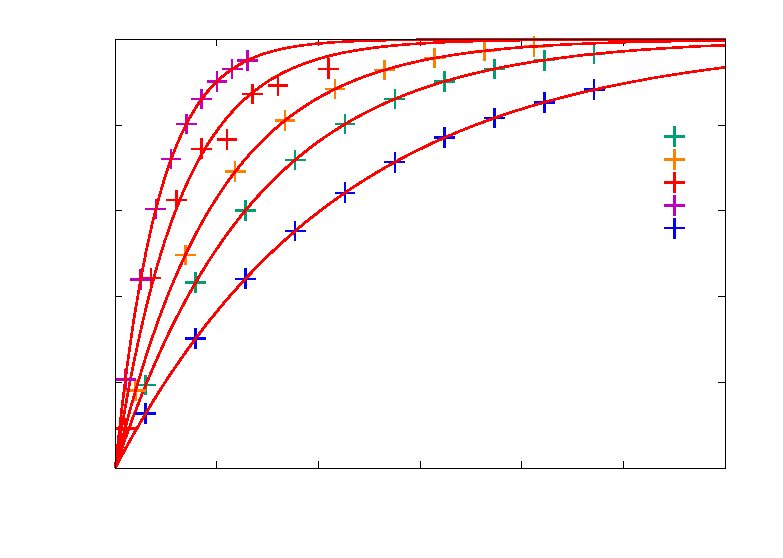
\includegraphics{plots/KupferalleT1}}%
    \gplfronttext
  \end{picture}%
\endgroup

    \caption{Alle Messungen T1 Cu2+}
\end{figure}
\begin{figure}[H]
    \centering
    % GNUPLOT: LaTeX picture with Postscript
\begingroup
  % Encoding inside the plot.  In the header of your document, this encoding
  % should to defined, e.g., by using
  % \usepackage[cp1252,<other encodings>]{inputenc}
  \inputencoding{cp1252}%
  \makeatletter
  \providecommand\color[2][]{%
    \GenericError{(gnuplot) \space\space\space\@spaces}{%
      Package color not loaded in conjunction with
      terminal option `colourtext'%
    }{See the gnuplot documentation for explanation.%
    }{Either use 'blacktext' in gnuplot or load the package
      color.sty in LaTeX.}%
    \renewcommand\color[2][]{}%
  }%
  \providecommand\includegraphics[2][]{%
    \GenericError{(gnuplot) \space\space\space\@spaces}{%
      Package graphicx or graphics not loaded%
    }{See the gnuplot documentation for explanation.%
    }{The gnuplot epslatex terminal needs graphicx.sty or graphics.sty.}%
    \renewcommand\includegraphics[2][]{}%
  }%
  \providecommand\rotatebox[2]{#2}%
  \@ifundefined{ifGPcolor}{%
    \newif\ifGPcolor
    \GPcolorfalse
  }{}%
  \@ifundefined{ifGPblacktext}{%
    \newif\ifGPblacktext
    \GPblacktexttrue
  }{}%
  % define a \g@addto@macro without @ in the name:
  \let\gplgaddtomacro\g@addto@macro
  % define empty templates for all commands taking text:
  \gdef\gplbacktext{}%
  \gdef\gplfronttext{}%
  \makeatother
  \ifGPblacktext
    % no textcolor at all
    \def\colorrgb#1{}%
    \def\colorgray#1{}%
  \else
    % gray or color?
    \ifGPcolor
      \def\colorrgb#1{\color[rgb]{#1}}%
      \def\colorgray#1{\color[gray]{#1}}%
      \expandafter\def\csname LTw\endcsname{\color{white}}%
      \expandafter\def\csname LTb\endcsname{\color{black}}%
      \expandafter\def\csname LTa\endcsname{\color{black}}%
      \expandafter\def\csname LT0\endcsname{\color[rgb]{1,0,0}}%
      \expandafter\def\csname LT1\endcsname{\color[rgb]{0,1,0}}%
      \expandafter\def\csname LT2\endcsname{\color[rgb]{0,0,1}}%
      \expandafter\def\csname LT3\endcsname{\color[rgb]{1,0,1}}%
      \expandafter\def\csname LT4\endcsname{\color[rgb]{0,1,1}}%
      \expandafter\def\csname LT5\endcsname{\color[rgb]{1,1,0}}%
      \expandafter\def\csname LT6\endcsname{\color[rgb]{0,0,0}}%
      \expandafter\def\csname LT7\endcsname{\color[rgb]{1,0.3,0}}%
      \expandafter\def\csname LT8\endcsname{\color[rgb]{0.5,0.5,0.5}}%
    \else
      % gray
      \def\colorrgb#1{\color{black}}%
      \def\colorgray#1{\color[gray]{#1}}%
      \expandafter\def\csname LTw\endcsname{\color{white}}%
      \expandafter\def\csname LTb\endcsname{\color{black}}%
      \expandafter\def\csname LTa\endcsname{\color{black}}%
      \expandafter\def\csname LT0\endcsname{\color{black}}%
      \expandafter\def\csname LT1\endcsname{\color{black}}%
      \expandafter\def\csname LT2\endcsname{\color{black}}%
      \expandafter\def\csname LT3\endcsname{\color{black}}%
      \expandafter\def\csname LT4\endcsname{\color{black}}%
      \expandafter\def\csname LT5\endcsname{\color{black}}%
      \expandafter\def\csname LT6\endcsname{\color{black}}%
      \expandafter\def\csname LT7\endcsname{\color{black}}%
      \expandafter\def\csname LT8\endcsname{\color{black}}%
    \fi
  \fi
    \setlength{\unitlength}{0.0500bp}%
    \ifx\gptboxheight\undefined%
      \newlength{\gptboxheight}%
      \newlength{\gptboxwidth}%
      \newsavebox{\gptboxtext}%
    \fi%
    \setlength{\fboxrule}{0.5pt}%
    \setlength{\fboxsep}{1pt}%
\begin{picture}(7200.00,5040.00)%
    \gplgaddtomacro\gplbacktext{%
      \csname LTb\endcsname%%
      \put(814,704){\makebox(0,0)[r]{\strut{}$0$}}%
      \put(814,1527){\makebox(0,0)[r]{\strut{}$0.2$}}%
      \put(814,2350){\makebox(0,0)[r]{\strut{}$0.4$}}%
      \put(814,3173){\makebox(0,0)[r]{\strut{}$0.6$}}%
      \put(814,3996){\makebox(0,0)[r]{\strut{}$0.8$}}%
      \put(814,4819){\makebox(0,0)[r]{\strut{}$1$}}%
      \put(946,484){\makebox(0,0){\strut{}$0$}}%
      \put(1922,484){\makebox(0,0){\strut{}$1000$}}%
      \put(2898,484){\makebox(0,0){\strut{}$2000$}}%
      \put(3875,484){\makebox(0,0){\strut{}$3000$}}%
      \put(4851,484){\makebox(0,0){\strut{}$4000$}}%
      \put(5827,484){\makebox(0,0){\strut{}$5000$}}%
      \put(6803,484){\makebox(0,0){\strut{}$6000$}}%
    }%
    \gplgaddtomacro\gplfronttext{%
      \csname LTb\endcsname%%
      \put(308,2761){\rotatebox{-270}{\makebox(0,0){\strut{}D\"ampfung $\frac{\text{E}}{\text{E}_0}$}}}%
      \put(3874,154){\makebox(0,0){\strut{}Zeit in $\si{\milli \second}$}}%
      \csname LTb\endcsname%%
      \put(5860,4606){\makebox(0,0)[r]{\strut{}$Cu^{2+} \SI{250}{\micro\mole}$}}%
      \csname LTb\endcsname%%
      \put(5860,4386){\makebox(0,0)[r]{\strut{}$Cu^{2+} \SI{1000}{\micro\mole}$}}%
      \csname LTb\endcsname%%
      \put(5860,4166){\makebox(0,0)[r]{\strut{}$Cu^{2+} \SI{250}{\micro\mole}$}}%
      \csname LTb\endcsname%%
      \put(5860,3946){\makebox(0,0)[r]{\strut{}$Cu^{2+} \SI{2000}{\micro\mole}$}}%
      \csname LTb\endcsname%%
      \put(5860,3726){\makebox(0,0)[r]{\strut{}Wasser}}%
    }%
    \gplbacktext
    \put(0,0){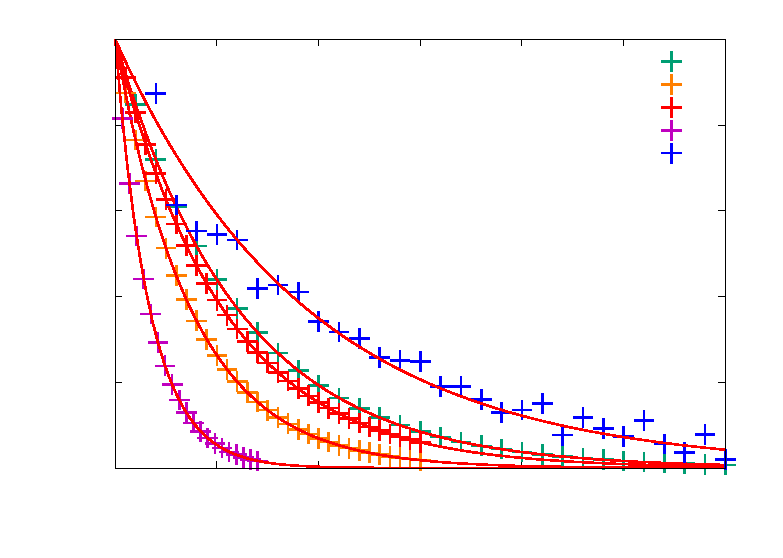
\includegraphics{plots/KupferalleT2}}%
    \gplfronttext
  \end{picture}%
\endgroup

    \caption{Alle Messungen T2Cu2+}
\end{figure}
\begin{figure}[H]
    \centering
    % GNUPLOT: LaTeX picture with Postscript
\begingroup
  % Encoding inside the plot.  In the header of your document, this encoding
  % should to defined, e.g., by using
  % \usepackage[cp1252,<other encodings>]{inputenc}
  \inputencoding{cp1252}%
  \makeatletter
  \providecommand\color[2][]{%
    \GenericError{(gnuplot) \space\space\space\@spaces}{%
      Package color not loaded in conjunction with
      terminal option `colourtext'%
    }{See the gnuplot documentation for explanation.%
    }{Either use 'blacktext' in gnuplot or load the package
      color.sty in LaTeX.}%
    \renewcommand\color[2][]{}%
  }%
  \providecommand\includegraphics[2][]{%
    \GenericError{(gnuplot) \space\space\space\@spaces}{%
      Package graphicx or graphics not loaded%
    }{See the gnuplot documentation for explanation.%
    }{The gnuplot epslatex terminal needs graphicx.sty or graphics.sty.}%
    \renewcommand\includegraphics[2][]{}%
  }%
  \providecommand\rotatebox[2]{#2}%
  \@ifundefined{ifGPcolor}{%
    \newif\ifGPcolor
    \GPcolorfalse
  }{}%
  \@ifundefined{ifGPblacktext}{%
    \newif\ifGPblacktext
    \GPblacktexttrue
  }{}%
  % define a \g@addto@macro without @ in the name:
  \let\gplgaddtomacro\g@addto@macro
  % define empty templates for all commands taking text:
  \gdef\gplbacktext{}%
  \gdef\gplfronttext{}%
  \makeatother
  \ifGPblacktext
    % no textcolor at all
    \def\colorrgb#1{}%
    \def\colorgray#1{}%
  \else
    % gray or color?
    \ifGPcolor
      \def\colorrgb#1{\color[rgb]{#1}}%
      \def\colorgray#1{\color[gray]{#1}}%
      \expandafter\def\csname LTw\endcsname{\color{white}}%
      \expandafter\def\csname LTb\endcsname{\color{black}}%
      \expandafter\def\csname LTa\endcsname{\color{black}}%
      \expandafter\def\csname LT0\endcsname{\color[rgb]{1,0,0}}%
      \expandafter\def\csname LT1\endcsname{\color[rgb]{0,1,0}}%
      \expandafter\def\csname LT2\endcsname{\color[rgb]{0,0,1}}%
      \expandafter\def\csname LT3\endcsname{\color[rgb]{1,0,1}}%
      \expandafter\def\csname LT4\endcsname{\color[rgb]{0,1,1}}%
      \expandafter\def\csname LT5\endcsname{\color[rgb]{1,1,0}}%
      \expandafter\def\csname LT6\endcsname{\color[rgb]{0,0,0}}%
      \expandafter\def\csname LT7\endcsname{\color[rgb]{1,0.3,0}}%
      \expandafter\def\csname LT8\endcsname{\color[rgb]{0.5,0.5,0.5}}%
    \else
      % gray
      \def\colorrgb#1{\color{black}}%
      \def\colorgray#1{\color[gray]{#1}}%
      \expandafter\def\csname LTw\endcsname{\color{white}}%
      \expandafter\def\csname LTb\endcsname{\color{black}}%
      \expandafter\def\csname LTa\endcsname{\color{black}}%
      \expandafter\def\csname LT0\endcsname{\color{black}}%
      \expandafter\def\csname LT1\endcsname{\color{black}}%
      \expandafter\def\csname LT2\endcsname{\color{black}}%
      \expandafter\def\csname LT3\endcsname{\color{black}}%
      \expandafter\def\csname LT4\endcsname{\color{black}}%
      \expandafter\def\csname LT5\endcsname{\color{black}}%
      \expandafter\def\csname LT6\endcsname{\color{black}}%
      \expandafter\def\csname LT7\endcsname{\color{black}}%
      \expandafter\def\csname LT8\endcsname{\color{black}}%
    \fi
  \fi
    \setlength{\unitlength}{0.0500bp}%
    \ifx\gptboxheight\undefined%
      \newlength{\gptboxheight}%
      \newlength{\gptboxwidth}%
      \newsavebox{\gptboxtext}%
    \fi%
    \setlength{\fboxrule}{0.5pt}%
    \setlength{\fboxsep}{1pt}%
\begin{picture}(7200.00,5040.00)%
    \gplgaddtomacro\gplbacktext{%
      \csname LTb\endcsname%%
      \put(814,704){\makebox(0,0)[r]{\strut{}$0$}}%
      \put(814,1527){\makebox(0,0)[r]{\strut{}$0.2$}}%
      \put(814,2350){\makebox(0,0)[r]{\strut{}$0.4$}}%
      \put(814,3173){\makebox(0,0)[r]{\strut{}$0.6$}}%
      \put(814,3996){\makebox(0,0)[r]{\strut{}$0.8$}}%
      \put(814,4819){\makebox(0,0)[r]{\strut{}$1$}}%
      \put(946,484){\makebox(0,0){\strut{}$0$}}%
      \put(1922,484){\makebox(0,0){\strut{}$1000$}}%
      \put(2898,484){\makebox(0,0){\strut{}$2000$}}%
      \put(3875,484){\makebox(0,0){\strut{}$3000$}}%
      \put(4851,484){\makebox(0,0){\strut{}$4000$}}%
      \put(5827,484){\makebox(0,0){\strut{}$5000$}}%
      \put(6803,484){\makebox(0,0){\strut{}$6000$}}%
    }%
    \gplgaddtomacro\gplfronttext{%
      \csname LTb\endcsname%%
      \put(198,2761){\rotatebox{-270}{\makebox(0,0){\strut{}D\"ampfung $\frac{\text{E}}{\text{E}_0}$}}}%
      \put(3874,154){\makebox(0,0){\strut{}Zeit in $\si{\milli \second}$}}%
      \csname LTb\endcsname%%
      \put(5860,3680){\makebox(0,0)[r]{\strut{}$Mn^{2+} \SI{25}{\micro\mole}$}}%
      \csname LTb\endcsname%%
      \put(5860,3460){\makebox(0,0)[r]{\strut{}$Mn^{2+} \SI{50}{\micro\mole}$}}%
      \csname LTb\endcsname%%
      \put(5860,3240){\makebox(0,0)[r]{\strut{}$Mn^{2+} \SI{100}{\micro\mole}$}}%
      \csname LTb\endcsname%%
      \put(5860,3020){\makebox(0,0)[r]{\strut{}$Mn^{2+} \SI{200}{\micro\mole}$}}%
      \csname LTb\endcsname%%
      \put(5860,2800){\makebox(0,0)[r]{\strut{}Wasser}}%
    }%
    \gplbacktext
    \put(0,0){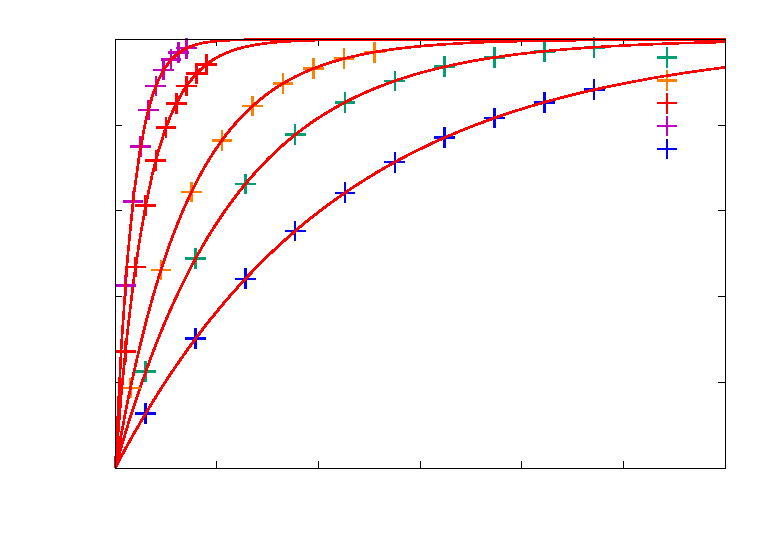
\includegraphics{plots/ManganalleT1}}%
    \gplfronttext
  \end{picture}%
\endgroup

    \caption{Alle Messungen T1Mn2+}
\end{figure}
\begin{figure}[H]
    \centering
    % GNUPLOT: LaTeX picture with Postscript
\begingroup
  % Encoding inside the plot.  In the header of your document, this encoding
  % should to defined, e.g., by using
  % \usepackage[cp1252,<other encodings>]{inputenc}
  \inputencoding{cp1252}%
  \makeatletter
  \providecommand\color[2][]{%
    \GenericError{(gnuplot) \space\space\space\@spaces}{%
      Package color not loaded in conjunction with
      terminal option `colourtext'%
    }{See the gnuplot documentation for explanation.%
    }{Either use 'blacktext' in gnuplot or load the package
      color.sty in LaTeX.}%
    \renewcommand\color[2][]{}%
  }%
  \providecommand\includegraphics[2][]{%
    \GenericError{(gnuplot) \space\space\space\@spaces}{%
      Package graphicx or graphics not loaded%
    }{See the gnuplot documentation for explanation.%
    }{The gnuplot epslatex terminal needs graphicx.sty or graphics.sty.}%
    \renewcommand\includegraphics[2][]{}%
  }%
  \providecommand\rotatebox[2]{#2}%
  \@ifundefined{ifGPcolor}{%
    \newif\ifGPcolor
    \GPcolorfalse
  }{}%
  \@ifundefined{ifGPblacktext}{%
    \newif\ifGPblacktext
    \GPblacktexttrue
  }{}%
  % define a \g@addto@macro without @ in the name:
  \let\gplgaddtomacro\g@addto@macro
  % define empty templates for all commands taking text:
  \gdef\gplbacktext{}%
  \gdef\gplfronttext{}%
  \makeatother
  \ifGPblacktext
    % no textcolor at all
    \def\colorrgb#1{}%
    \def\colorgray#1{}%
  \else
    % gray or color?
    \ifGPcolor
      \def\colorrgb#1{\color[rgb]{#1}}%
      \def\colorgray#1{\color[gray]{#1}}%
      \expandafter\def\csname LTw\endcsname{\color{white}}%
      \expandafter\def\csname LTb\endcsname{\color{black}}%
      \expandafter\def\csname LTa\endcsname{\color{black}}%
      \expandafter\def\csname LT0\endcsname{\color[rgb]{1,0,0}}%
      \expandafter\def\csname LT1\endcsname{\color[rgb]{0,1,0}}%
      \expandafter\def\csname LT2\endcsname{\color[rgb]{0,0,1}}%
      \expandafter\def\csname LT3\endcsname{\color[rgb]{1,0,1}}%
      \expandafter\def\csname LT4\endcsname{\color[rgb]{0,1,1}}%
      \expandafter\def\csname LT5\endcsname{\color[rgb]{1,1,0}}%
      \expandafter\def\csname LT6\endcsname{\color[rgb]{0,0,0}}%
      \expandafter\def\csname LT7\endcsname{\color[rgb]{1,0.3,0}}%
      \expandafter\def\csname LT8\endcsname{\color[rgb]{0.5,0.5,0.5}}%
    \else
      % gray
      \def\colorrgb#1{\color{black}}%
      \def\colorgray#1{\color[gray]{#1}}%
      \expandafter\def\csname LTw\endcsname{\color{white}}%
      \expandafter\def\csname LTb\endcsname{\color{black}}%
      \expandafter\def\csname LTa\endcsname{\color{black}}%
      \expandafter\def\csname LT0\endcsname{\color{black}}%
      \expandafter\def\csname LT1\endcsname{\color{black}}%
      \expandafter\def\csname LT2\endcsname{\color{black}}%
      \expandafter\def\csname LT3\endcsname{\color{black}}%
      \expandafter\def\csname LT4\endcsname{\color{black}}%
      \expandafter\def\csname LT5\endcsname{\color{black}}%
      \expandafter\def\csname LT6\endcsname{\color{black}}%
      \expandafter\def\csname LT7\endcsname{\color{black}}%
      \expandafter\def\csname LT8\endcsname{\color{black}}%
    \fi
  \fi
    \setlength{\unitlength}{0.0500bp}%
    \ifx\gptboxheight\undefined%
      \newlength{\gptboxheight}%
      \newlength{\gptboxwidth}%
      \newsavebox{\gptboxtext}%
    \fi%
    \setlength{\fboxrule}{0.5pt}%
    \setlength{\fboxsep}{1pt}%
\begin{picture}(7200.00,5040.00)%
    \gplgaddtomacro\gplbacktext{%
      \csname LTb\endcsname%%
      \put(814,704){\makebox(0,0)[r]{\strut{}$0$}}%
      \put(814,1527){\makebox(0,0)[r]{\strut{}$0.2$}}%
      \put(814,2350){\makebox(0,0)[r]{\strut{}$0.4$}}%
      \put(814,3173){\makebox(0,0)[r]{\strut{}$0.6$}}%
      \put(814,3996){\makebox(0,0)[r]{\strut{}$0.8$}}%
      \put(814,4819){\makebox(0,0)[r]{\strut{}$1$}}%
      \put(946,484){\makebox(0,0){\strut{}$0$}}%
      \put(1922,484){\makebox(0,0){\strut{}$1000$}}%
      \put(2898,484){\makebox(0,0){\strut{}$2000$}}%
      \put(3875,484){\makebox(0,0){\strut{}$3000$}}%
      \put(4851,484){\makebox(0,0){\strut{}$4000$}}%
      \put(5827,484){\makebox(0,0){\strut{}$5000$}}%
      \put(6803,484){\makebox(0,0){\strut{}$6000$}}%
    }%
    \gplgaddtomacro\gplfronttext{%
      \csname LTb\endcsname%%
      \put(198,2761){\rotatebox{-270}{\makebox(0,0){\strut{}D\"ampfung $\frac{\text{E}}{\text{E}_0}$}}}%
      \put(3874,154){\makebox(0,0){\strut{}Zeit in $\si{\milli \second}$}}%
      \csname LTb\endcsname%%
      \put(5860,4606){\makebox(0,0)[r]{\strut{}$Mn^{2+} \SI{25}{\micro\mole}$}}%
      \csname LTb\endcsname%%
      \put(5860,4386){\makebox(0,0)[r]{\strut{}$Mn^{2+} \SI{100}{\micro\mole}$}}%
      \csname LTb\endcsname%%
      \put(5860,4166){\makebox(0,0)[r]{\strut{}$Mn^{2+} \SI{25}{\micro\mole}$}}%
      \csname LTb\endcsname%%
      \put(5860,3946){\makebox(0,0)[r]{\strut{}$Mn^{2+} \SI{200}{\micro\mole}$}}%
      \csname LTb\endcsname%%
      \put(5860,3726){\makebox(0,0)[r]{\strut{}Wasser}}%
    }%
    \gplbacktext
    \put(0,0){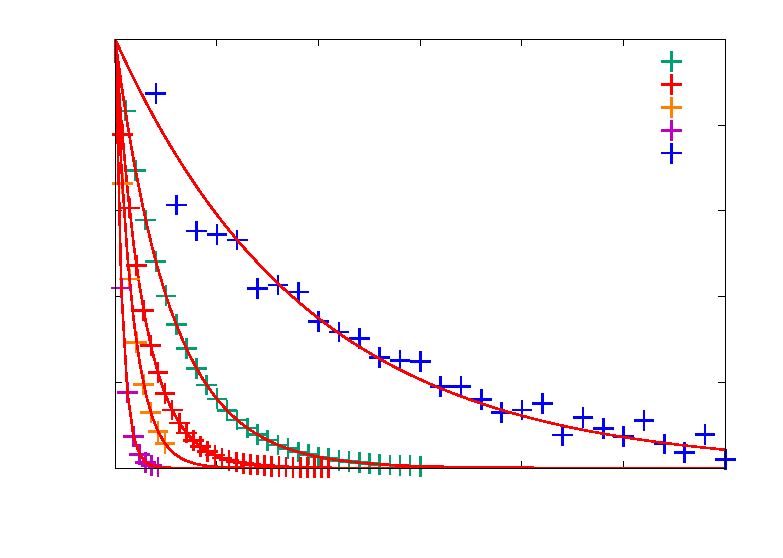
\includegraphics{plots/ManganalleT2}}%
    \gplfronttext
  \end{picture}%
\endgroup

    \caption{Alle Messungen T2MN2+}
\end{figure}

\begin{table}[H]
    \centering]
    \begin{tabular}{lllll}
    \hline
    \multicolumn{1}{|l|}{}            & \multicolumn{1}{l|}{T1}      & \multicolumn{1}{l|}{U(T1)-Fit} & \multicolumn{1}{l|}{T2}      & \multicolumn{1}{l|}{U(T2)-Fit}  \\ \hline
    \multicolumn{1}{|l|}{Cu2    250}  & \multicolumn{1}{l|}{1394,84} & \multicolumn{1}{l|}{0,001055}  & \multicolumn{1}{l|}{1215,51} & \multicolumn{1}{l|}{0,0002529}  \\ \hline
    \multicolumn{1}{|l|}{Cu2    500}  & \multicolumn{1}{l|}{1003,4}  & \multicolumn{1}{l|}{0,0004851} & \multicolumn{1}{l|}{1066,44} & \multicolumn{1}{l|}{0,0002621}  \\ \hline
    \multicolumn{1}{|l|}{Cu2    1000} & \multicolumn{1}{l|}{646,849} & \multicolumn{1}{l|}{71,54}     & \multicolumn{1}{l|}{748,404} & \multicolumn{1}{l|}{0,0001937}  \\ \hline
    \multicolumn{1}{|l|}{Cu2    2000} & \multicolumn{1}{l|}{431,268} & \multicolumn{1}{l|}{0,0002906} & \multicolumn{1}{l|}{341,83}  & \multicolumn{1}{l|}{0,0001228}  \\ \hline
                                      &                              &                                &                              &                                 \\ \hline
    \multicolumn{1}{|l|}{}            & \multicolumn{1}{l|}{T1}      & \multicolumn{1}{l|}{U(T1)-Fit} & \multicolumn{1}{l|}{T2}      & \multicolumn{1}{l|}{U(T2)-Fit}  \\ \hline
    \multicolumn{1}{|l|}{Wasser}      & \multicolumn{1}{l|}{2199,46} & \multicolumn{1}{l|}{0,003027}  & \multicolumn{1}{l|}{1901,06} & \multicolumn{1}{l|}{89,83}      \\ \hline
                                      &                              &                                &                              &                                 \\
                                      &                              &                                &                              &                                 \\ \hline
    \multicolumn{1}{|l|}{}            & \multicolumn{1}{l|}{T1}      & \multicolumn{1}{l|}{U(T1)-Fit} & \multicolumn{1}{l|}{T2}      & \multicolumn{1}{l|}{U(T2)-Fit}  \\ \hline
    \multicolumn{1}{|l|}{Mn 2 25}     & \multicolumn{1}{l|}{1178,28} & \multicolumn{1}{l|}{0,0009801} & \multicolumn{1}{l|}{548,337} & \multicolumn{1}{l|}{0,0001258}  \\ \hline
    \multicolumn{1}{|l|}{Mn 2 50}     & \multicolumn{1}{l|}{725,857} & \multicolumn{1}{l|}{0,0006027} & \multicolumn{1}{l|}{279,858} & \multicolumn{1}{l|}{0,00008179} \\ \hline
    \multicolumn{1}{|l|}{Mn 2 100}    & \multicolumn{1}{l|}{316,085} & \multicolumn{1}{l|}{0,0003079} & \multicolumn{1}{l|}{170,996} & \multicolumn{1}{l|}{0,0001182}  \\ \hline
    \multicolumn{1}{|l|}{Mn 2 200}    & \multicolumn{1}{l|}{180,244} & \multicolumn{1}{l|}{0,0001274} & \multicolumn{1}{l|}{69,1512} & \multicolumn{1}{l|}{0,0000547}  \\ \hline
    \end{tabular}
    \caption{T1- und T2- abhängig von den Stoffen und der Konzentration}
    \end{table}
% !TEX root = main.tex
\subsection{1D MRI}
\label{sec:1DMRIkapitel}
Bei dem MRI-Verfahren wird neben dem Erdmagnetfeld $B_0$ ein Gradientenfeld \textbf{G} angelegt.
Somit ist die Larmorfrequenz nicht nur durch $B_0$ gegeben.
Es muss zusätzlich noch das angelegte Gradientenfeld mitbetrachtet werden.
Falls man dies speziell in x-Richtung (also $G_xx$) betrachtet, so kann die Larmorfrequenz wie folgt ausgedrückt werden:
\begin{align}
    \omega(x)=\gamma |B(x)|= \gamma \left(B_0+G_xx\right) \label{eq:gradientlarmor}
\end{align}
Aus dieser Formel geht nun hervor, dass jeder Spin ein vom Ort abhängiges Magnetfeld erfährt.
Somit besitzt jeder Spin eine andere Larmorfrequenz.
Diese präzidieren mit unterschiedlicher Geschwidigkeiten womit dann auf den Ort des Spins zurück geschlossen werden kann. \\

Die Grundidee wie dies am Ende gemesen wird liegt darin, dass man im Fourieraum ein Spektrum erhälten, indem Datenpunkte in Abhängigkeit von der Zeit gemessen werden und diese dann integriert werden.
Für die positiven Zeiten stellt dies kein Problem dar.
Jedoch wird bei der Fourietransformation auch über die negative Zeiten integriert, die nicht gemessen werden können.
Die Lösung dieses Problemes liegt darin, dass als erstes ein negatives Gradientenfeld $-G$ angelegt wird.
Was dies anschaulich bedeutet, kann in der folgenden Abbildung \ref{fig:1DMRI} sichtbar gemacht werden.  
\begin{figure}[H]
    \centering
    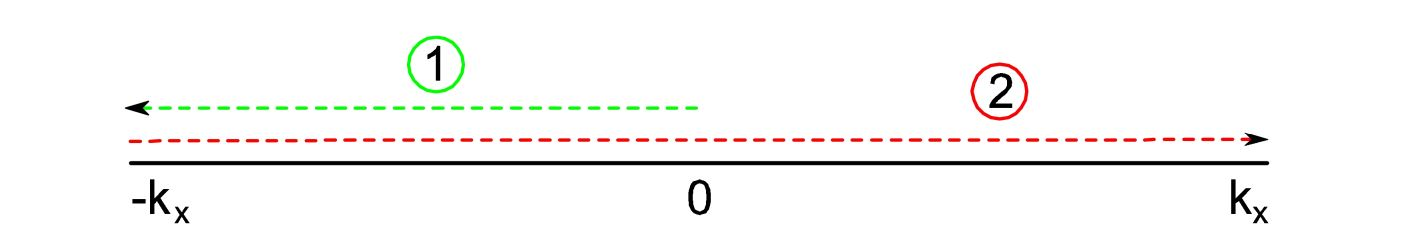
\includegraphics[width=0.8\textwidth]{Abbildungen/1DMRIkraum.JPG}
    \caption[Veranschaulichter Verlauf des k-Vektors im 1D-MRI]{Diese Abbildung dient zur Veranschaulichung der Messmethode im k-Raum.
    In Schritt 1 wird als erstes ein negativer Gradient angelegt, sodass im k-Raum der k-Vektor verringert wird.
    Das negative Gradientenfeld wird nun so lange angelegt, bis man die erwünschte Bandbreite in $-k_{x}$-Richtung erreicht hat.
    Sobald dies geschehen ist, wird das gleiche Gradientenfeld nur in positiver Richtung nochmal angelegt.
    Dies passiert so lange,  bis man im k-Raum die erwünschte Bandbreite von $-k_{x}$ bis $k_{x}$ erreicht hat.
    Das Signal wird hierbei während dem Vorgang (2) gemessen.\cite{Schmidt}}
    \label{fig:1DMRI}
\end{figure}

Als erstes wurde ein 1D-MRI in Richtung von der x-Achse gemessen.
Im folgenden werden nun zwei Messungen miteinander verglichen, die mit unterschiedlichen Parametern vermessen wurden.  
\begin{figure}[H]
    \centering
    % GNUPLOT: LaTeX picture with Postscript
\begingroup
  % Encoding inside the plot.  In the header of your document, this encoding
  % should to defined, e.g., by using
  % \usepackage[cp1252,<other encodings>]{inputenc}
  \inputencoding{cp1252}%
  \makeatletter
  \providecommand\color[2][]{%
    \GenericError{(gnuplot) \space\space\space\@spaces}{%
      Package color not loaded in conjunction with
      terminal option `colourtext'%
    }{See the gnuplot documentation for explanation.%
    }{Either use 'blacktext' in gnuplot or load the package
      color.sty in LaTeX.}%
    \renewcommand\color[2][]{}%
  }%
  \providecommand\includegraphics[2][]{%
    \GenericError{(gnuplot) \space\space\space\@spaces}{%
      Package graphicx or graphics not loaded%
    }{See the gnuplot documentation for explanation.%
    }{The gnuplot epslatex terminal needs graphicx.sty or graphics.sty.}%
    \renewcommand\includegraphics[2][]{}%
  }%
  \providecommand\rotatebox[2]{#2}%
  \@ifundefined{ifGPcolor}{%
    \newif\ifGPcolor
    \GPcolorfalse
  }{}%
  \@ifundefined{ifGPblacktext}{%
    \newif\ifGPblacktext
    \GPblacktexttrue
  }{}%
  % define a \g@addto@macro without @ in the name:
  \let\gplgaddtomacro\g@addto@macro
  % define empty templates for all commands taking text:
  \gdef\gplbacktext{}%
  \gdef\gplfronttext{}%
  \makeatother
  \ifGPblacktext
    % no textcolor at all
    \def\colorrgb#1{}%
    \def\colorgray#1{}%
  \else
    % gray or color?
    \ifGPcolor
      \def\colorrgb#1{\color[rgb]{#1}}%
      \def\colorgray#1{\color[gray]{#1}}%
      \expandafter\def\csname LTw\endcsname{\color{white}}%
      \expandafter\def\csname LTb\endcsname{\color{black}}%
      \expandafter\def\csname LTa\endcsname{\color{black}}%
      \expandafter\def\csname LT0\endcsname{\color[rgb]{1,0,0}}%
      \expandafter\def\csname LT1\endcsname{\color[rgb]{0,1,0}}%
      \expandafter\def\csname LT2\endcsname{\color[rgb]{0,0,1}}%
      \expandafter\def\csname LT3\endcsname{\color[rgb]{1,0,1}}%
      \expandafter\def\csname LT4\endcsname{\color[rgb]{0,1,1}}%
      \expandafter\def\csname LT5\endcsname{\color[rgb]{1,1,0}}%
      \expandafter\def\csname LT6\endcsname{\color[rgb]{0,0,0}}%
      \expandafter\def\csname LT7\endcsname{\color[rgb]{1,0.3,0}}%
      \expandafter\def\csname LT8\endcsname{\color[rgb]{0.5,0.5,0.5}}%
    \else
      % gray
      \def\colorrgb#1{\color{black}}%
      \def\colorgray#1{\color[gray]{#1}}%
      \expandafter\def\csname LTw\endcsname{\color{white}}%
      \expandafter\def\csname LTb\endcsname{\color{black}}%
      \expandafter\def\csname LTa\endcsname{\color{black}}%
      \expandafter\def\csname LT0\endcsname{\color{black}}%
      \expandafter\def\csname LT1\endcsname{\color{black}}%
      \expandafter\def\csname LT2\endcsname{\color{black}}%
      \expandafter\def\csname LT3\endcsname{\color{black}}%
      \expandafter\def\csname LT4\endcsname{\color{black}}%
      \expandafter\def\csname LT5\endcsname{\color{black}}%
      \expandafter\def\csname LT6\endcsname{\color{black}}%
      \expandafter\def\csname LT7\endcsname{\color{black}}%
      \expandafter\def\csname LT8\endcsname{\color{black}}%
    \fi
  \fi
    \setlength{\unitlength}{0.0500bp}%
    \ifx\gptboxheight\undefined%
      \newlength{\gptboxheight}%
      \newlength{\gptboxwidth}%
      \newsavebox{\gptboxtext}%
    \fi%
    \setlength{\fboxrule}{0.5pt}%
    \setlength{\fboxsep}{1pt}%
\begin{picture}(7200.00,5040.00)%
    \gplgaddtomacro\gplbacktext{%
      \csname LTb\endcsname%%
      \put(1078,704){\makebox(0,0)[r]{\strut{}$0$}}%
      \put(1078,1292){\makebox(0,0)[r]{\strut{}$5000$}}%
      \put(1078,1880){\makebox(0,0)[r]{\strut{}$10000$}}%
      \put(1078,2468){\makebox(0,0)[r]{\strut{}$15000$}}%
      \put(1078,3055){\makebox(0,0)[r]{\strut{}$20000$}}%
      \put(1078,3643){\makebox(0,0)[r]{\strut{}$25000$}}%
      \put(1078,4231){\makebox(0,0)[r]{\strut{}$30000$}}%
      \put(1078,4819){\makebox(0,0)[r]{\strut{}$35000$}}%
      \put(1385,484){\makebox(0,0){\strut{}$-30$}}%
      \put(2259,484){\makebox(0,0){\strut{}$-20$}}%
      \put(3133,484){\makebox(0,0){\strut{}$-10$}}%
      \put(4007,484){\makebox(0,0){\strut{}$0$}}%
      \put(4880,484){\makebox(0,0){\strut{}$10$}}%
      \put(5754,484){\makebox(0,0){\strut{}$20$}}%
      \put(6628,484){\makebox(0,0){\strut{}$30$}}%
    }%
    \gplgaddtomacro\gplfronttext{%
      \csname LTb\endcsname%%
      \put(198,2761){\rotatebox{-270}{\makebox(0,0){\strut{}Amplitude in $\si{\milli \second}$}}}%
      \put(4006,154){\makebox(0,0){\strut{}Frequenz in $\si{\hertz}$}}%
      \csname LTb\endcsname%%
      \put(5816,4646){\makebox(0,0)[r]{\strut{}1D-MRI Messung, angepasste FOV und Bandbreite  }}%
    }%
    \gplbacktext
    \put(0,0){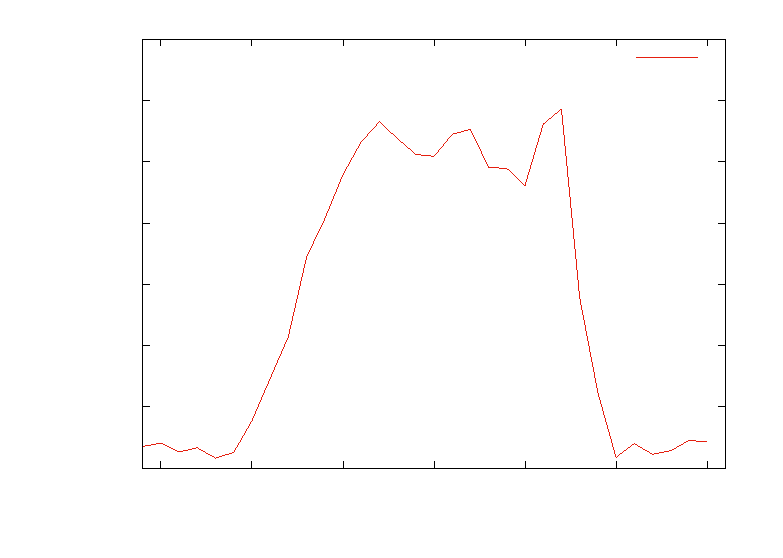
\includegraphics{plots/1DMRI}}%
    \gplfronttext
  \end{picture}%
\endgroup

    \caption[1D-MRI in x-Richtung nach Anpassung der FOV und Bandbreite]{1D-MRI in x-Richtung nach Anpassung der FOV und Bandbreite. Aus dieser Abbildung wurde eine Länge des Phantoms von $l=\SI{15,65}{\centi\m}$ ermittelt. Ein Peak ist bei ca. $\SI{13}{\hertz}$ zu sehen, welches auf ein Vielfaches der deutschen Netzspannung ($\SI{50}{\hertz}$) ergibt, da es sich hierbei um $\SI{1850}{\hertz}$. Es ist ein steiler Anstieg/Abfall um $\pm \SI{20}{\hertz}$ zu sehen, was auf eine \glqq rechteckige\grqq Form des Objektes entlang der x-Achse schließen lässt.\label{fig:1Dx}}
\end{figure}
% In der Abbildung \ref{fig:1Dx} kann man große unterschiede zwischen den beiden Messungen sehen. Es ist hierbei schwer aus der ersten Messung gute Informationen über das Phantom heraus zu bekommen. Es ist kein klarer Abfall zu sehen, weshalb man daraus nicht die Abmessung des Phantomes herausbekommen kann.
In der Abbildung \ref{fig:1Dx} ist zu sehen, dass bei $\SI{-20}{\hertz}$ und $\SI{20}{\hertz}$ ein starker Anstieg/Abfall des Signals stattfindet. Dies lässt sich dadurch erklären, dass durch die räumliche Ausdehnung des Phantoms die Spins an unterschiedlichen Orten eine andere Larmorfrequenz besitzten. Ursache hierfür ist das Gradientenfeld, welches während dem Messvorgang angelegt ist. Diese unterschiedlichen Larmorfrequenzen stellen das \glqq Plateau\grqq \, dar, was zwischen $\SI{-20}{\hertz}$ und $\SI{20}{\hertz}$ vorhanden ist.\\
Anhand dieses Signales kann  nun auch die Größe des Objektes ermittelt werden. Hierzu wird die Formel \ref{eq:gradientlarmor} benutzt um $\Delta x$ zu berechnen. Hierbei wird $\Delta\omega= 2\pi \Delta f$ umgerechnet, sodass man die folgende Formel erhält:
\begin{align}
    \Delta x&=\frac{\Delta\omega}{\gamma G_x}\\
    \Delta x&=\frac{\Delta f \cdot 2\pi}{\gamma G_x}\\
\end{align}\label{eq:FOV}
Aus der Abbildung kann die Bandbreite von ca. $\SI{40}{\hertz}$ ermittelt werden. Das gyromagnetische Moment von $\SI{2.67e8}{\s^{-1}\tesla^{-1}}$ wurde aus \cite{Schmidt} entnommen und der Gradient $G_x=\SI{6,0}{\frac{\mu\tesla}{\m}}$ wurde am Versuchstag im Messprotokoll festgehalten. Mit diesen Daten bekommt man für die Länge des Phantomes $l=\SI{15,65}{\centi\m}$ heraus.\\
Neben der Bandbreite kann in der Abbildung beobeachtet werden, dass bei ca. $\SI{13}{\hertz}$ ein kleiner Peak zu sehen ist.(Dieser Peak ist wesentlich deutlicher noch in Abb. \ref{fig:1Dy} zu sehen). Der Ursprung dieser Peaks liegt an der deutschen Netzspannung, die mit $\SI{50}{\hertz}$ getaktet ist. Wenn man sich nun den Urprung anschaut, so liegt dieser bei der Larmorfrequenz von $\SI{1837,27}{\hertz}$, die am ersten Versuchstag vermessen wurde. Wenn dazu noch $\SI{13}{\hertz}$ hinzu addiert werden, so  kommt man zu dem Schluss, dass die Peaks bei $\SI{1850}{\hertz}$ liegen und somit ein Vielfaches von der Netzspannung sind.\\
Wie schon im vorherigen Absatz angesprochen, wurde im Anschluss eine weitere MRI Messung gemacht, die sich jedoch entlang der y-Achse orientiert hat. Die Messung wird nun in der folgenden Abbildung dargestellt.
\begin{figure}[H]
    \centering
    % GNUPLOT: LaTeX picture with Postscript
\begingroup
  % Encoding inside the plot.  In the header of your document, this encoding
  % should to defined, e.g., by using
  % \usepackage[cp1252,<other encodings>]{inputenc}
  \inputencoding{cp1252}%
  \makeatletter
  \providecommand\color[2][]{%
    \GenericError{(gnuplot) \space\space\space\@spaces}{%
      Package color not loaded in conjunction with
      terminal option `colourtext'%
    }{See the gnuplot documentation for explanation.%
    }{Either use 'blacktext' in gnuplot or load the package
      color.sty in LaTeX.}%
    \renewcommand\color[2][]{}%
  }%
  \providecommand\includegraphics[2][]{%
    \GenericError{(gnuplot) \space\space\space\@spaces}{%
      Package graphicx or graphics not loaded%
    }{See the gnuplot documentation for explanation.%
    }{The gnuplot epslatex terminal needs graphicx.sty or graphics.sty.}%
    \renewcommand\includegraphics[2][]{}%
  }%
  \providecommand\rotatebox[2]{#2}%
  \@ifundefined{ifGPcolor}{%
    \newif\ifGPcolor
    \GPcolorfalse
  }{}%
  \@ifundefined{ifGPblacktext}{%
    \newif\ifGPblacktext
    \GPblacktexttrue
  }{}%
  % define a \g@addto@macro without @ in the name:
  \let\gplgaddtomacro\g@addto@macro
  % define empty templates for all commands taking text:
  \gdef\gplbacktext{}%
  \gdef\gplfronttext{}%
  \makeatother
  \ifGPblacktext
    % no textcolor at all
    \def\colorrgb#1{}%
    \def\colorgray#1{}%
  \else
    % gray or color?
    \ifGPcolor
      \def\colorrgb#1{\color[rgb]{#1}}%
      \def\colorgray#1{\color[gray]{#1}}%
      \expandafter\def\csname LTw\endcsname{\color{white}}%
      \expandafter\def\csname LTb\endcsname{\color{black}}%
      \expandafter\def\csname LTa\endcsname{\color{black}}%
      \expandafter\def\csname LT0\endcsname{\color[rgb]{1,0,0}}%
      \expandafter\def\csname LT1\endcsname{\color[rgb]{0,1,0}}%
      \expandafter\def\csname LT2\endcsname{\color[rgb]{0,0,1}}%
      \expandafter\def\csname LT3\endcsname{\color[rgb]{1,0,1}}%
      \expandafter\def\csname LT4\endcsname{\color[rgb]{0,1,1}}%
      \expandafter\def\csname LT5\endcsname{\color[rgb]{1,1,0}}%
      \expandafter\def\csname LT6\endcsname{\color[rgb]{0,0,0}}%
      \expandafter\def\csname LT7\endcsname{\color[rgb]{1,0.3,0}}%
      \expandafter\def\csname LT8\endcsname{\color[rgb]{0.5,0.5,0.5}}%
    \else
      % gray
      \def\colorrgb#1{\color{black}}%
      \def\colorgray#1{\color[gray]{#1}}%
      \expandafter\def\csname LTw\endcsname{\color{white}}%
      \expandafter\def\csname LTb\endcsname{\color{black}}%
      \expandafter\def\csname LTa\endcsname{\color{black}}%
      \expandafter\def\csname LT0\endcsname{\color{black}}%
      \expandafter\def\csname LT1\endcsname{\color{black}}%
      \expandafter\def\csname LT2\endcsname{\color{black}}%
      \expandafter\def\csname LT3\endcsname{\color{black}}%
      \expandafter\def\csname LT4\endcsname{\color{black}}%
      \expandafter\def\csname LT5\endcsname{\color{black}}%
      \expandafter\def\csname LT6\endcsname{\color{black}}%
      \expandafter\def\csname LT7\endcsname{\color{black}}%
      \expandafter\def\csname LT8\endcsname{\color{black}}%
    \fi
  \fi
    \setlength{\unitlength}{0.0500bp}%
    \ifx\gptboxheight\undefined%
      \newlength{\gptboxheight}%
      \newlength{\gptboxwidth}%
      \newsavebox{\gptboxtext}%
    \fi%
    \setlength{\fboxrule}{0.5pt}%
    \setlength{\fboxsep}{1pt}%
\begin{picture}(7200.00,5040.00)%
    \gplgaddtomacro\gplbacktext{%
      \csname LTb\endcsname%%
      \put(1078,704){\makebox(0,0)[r]{\strut{}$0$}}%
      \put(1078,1260){\makebox(0,0)[r]{\strut{}$5000$}}%
      \put(1078,1816){\makebox(0,0)[r]{\strut{}$10000$}}%
      \put(1078,2372){\makebox(0,0)[r]{\strut{}$15000$}}%
      \put(1078,2928){\makebox(0,0)[r]{\strut{}$20000$}}%
      \put(1078,3484){\makebox(0,0)[r]{\strut{}$25000$}}%
      \put(1078,4040){\makebox(0,0)[r]{\strut{}$30000$}}%
      \put(1078,4597){\makebox(0,0)[r]{\strut{}$35000$}}%
      \put(1539,484){\makebox(0,0){\strut{}$-15$}}%
      \put(2362,484){\makebox(0,0){\strut{}$-10$}}%
      \put(3184,484){\makebox(0,0){\strut{}$-5$}}%
      \put(4007,484){\makebox(0,0){\strut{}$0$}}%
      \put(4829,484){\makebox(0,0){\strut{}$5$}}%
      \put(5652,484){\makebox(0,0){\strut{}$10$}}%
      \put(6474,484){\makebox(0,0){\strut{}$15$}}%
    }%
    \gplgaddtomacro\gplfronttext{%
      \csname LTb\endcsname%%
      \put(198,2761){\rotatebox{-270}{\makebox(0,0){\strut{}Amplitude in $\si{\milli \second}$}}}%
      \put(4006,154){\makebox(0,0){\strut{}Frequenz in $\si{\hertz}$}}%
      \csname LTb\endcsname%%
      \put(5816,4646){\makebox(0,0)[r]{\strut{}erste 1D MRI Messung in yRichtung}}%
      \csname LTb\endcsname%%
      \put(5816,4426){\makebox(0,0)[r]{\strut{}zweite 1D MRI Messung mit ver\"anderter5 Bandbreite}}%
    }%
    \gplbacktext
    \put(0,0){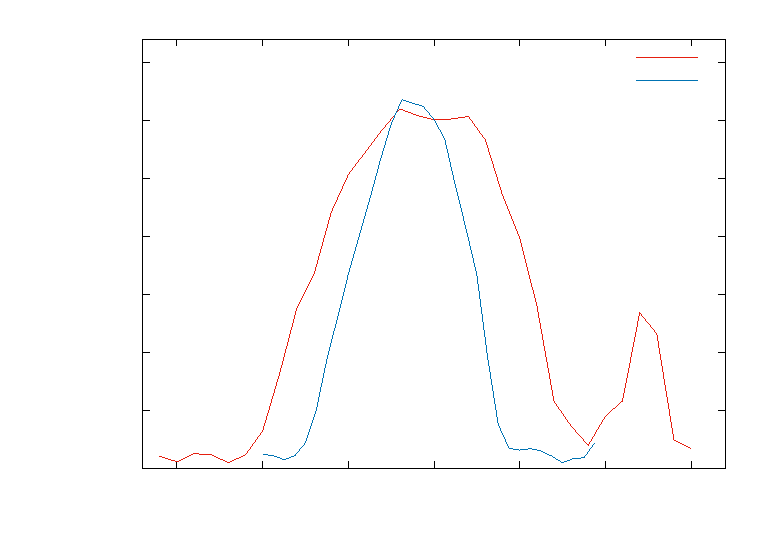
\includegraphics{plots/1DMRIy}}%
    \gplfronttext
  \end{picture}%
\endgroup

    \caption[1-MRI in y-Richtung nach Anpassung der FOV]{1-MRI in y-Richtung nach Anpassung der FOV. Hier wurde eine Breite von $b=\SI{6,57}{\centi \m}$ bwatimmt. Der Anstieg/Abfall ist nicht steil, was eher auf eine runde Form des Phantoms spricht entlang der y-Achse}\label{fig:1Dy}
\end{figure} 
Auch hier kann beobachtet werden, dass die räumliche Ausdehnung der Probe zu einer Erhöhung des Signals führt. Die Breite des Phantoms $b=\SI{6,57}{\centi \m}$ wurde analog zu der Formel \ref{eq:FOV} wie vorhin berechnet. Wenn die Signale in x,y-Richtung verglichen werden, so sieht man tendenziell, dass das Signal entlang der x-Richtung schneller bzw. stärker ansteigt/abfällt. Dies könnte unter anderem mit der Form des Phantoms zusammen hängen. Hierbei würde ein starker Abfall eher auf eine eckige Form zutreffen und eine schwächerer Abfall würde eher auf eine runde Form zutreffen. Mit diesem Wissen kann man die Vermutung aufstellen, dass das Phantom ein Zylinder sein kann. Dies würde erklären, dass entlang der x-Richtung der Graph stärker abflällt, da ein Zylinder entlang der Höhe einem Rechteck ähnlicher sieht als einer Kugel oder einem Kreis. Wenn jedoch die Grundfläche in der y,z-Ebene betrachtet wird, so handelt es sich hierbei um einen Kreis. Dies würde erklären, warum das Signal in y-Richtung schwächer ansteigt/abfällt. Wenn man mit diesem Wissen das Volumen des Zylinders mit der ermittelten Länge und der Breite berechnet, so erhält man ein Volumen $V=\SI{532}{\milli\liter}$.\\
In anderen Versuchsteilen wurde ein ähnliches Objekt verwendet, welches ein Volumen von $\SI{500}{\milli \liter}$ hatte. Die Vermutung liegt nahe, dass das untersuchte Phantom die gleiche Abmessung hatte und ebenfalls mit Wasser gefüllt war. Die Abweichung von $\SI{32}{\milli\liter}$ können durch Messunsicherheiten erklärt werden.\\
Eine mögliche Quelle für eine Unsicherheit kann durch das Auflösungsvermögen entstehen. Das Auflösungsvermögen ist durch $\Delta x=\frac{FOV}{N}$ gegeben, wobei N die Anzahl der Pixels darstellt\cite{Schmidt}. Nun könnte man diesen Wert bestimmen, aber dies würde aus zwei Gründen nicht so viel Sinn machen. Zum einen wäre es der Fakt, dass zwar ein Wert ermittelt werden kann, aber da es keine Referenzwerte gibt, womit man entscheiden könnte, ob dies eine gute Auflösung ist oder nicht, wurde dies nicht gemacht. Der andere Grund, warum dies nicht explizit berechnet wurde liegt daran, dass es meist auch andere Faktoren gibt, die bei der tatsächlichen Auflösung eine Rolle spielen. Hierbei kann es sein, dass zwischen den einzelnen Pixels es zu einer unschärfe kommt, wodurch die Auflösung dann gröber wird.\\
Ein weiteres Problem stellt sich bei der Auswertung heraus. Hierbei ist es schwierig, genau zu identifizieren, wo genau das Phantom aufhört bzw. die Bandbreite zu bestimmen. Hier muss man darauf ahcten, dass das Signal von der Netztfrequenz oder auch von dem Rauschen nicht dazu genommen werden soll. Vor allem in der ersten Abbildung stellt dies ein Problem dar, da sich das Phantom mit dem Peak der Netzfrequenz überschneidet.
Wenn man die Unsicherheit kleiner haben möchte, dann kann man versuchen die Auflösung zu verbessern indem man die FOV (den Bereich den man anschaut) kleiner wählt und somit nur das Phantom vermisst. Darauf wurde am Versuchstag schon geachtet, dass dies möglichst gut eingehalten wird. \\
Eine weiter Möglichkeit das Signal zu verbessern besteht darin, indem man mehrere Messungen hintereinander macht. Dadurch hätte man mehr Datenpunkte zur Verfügung, womit man ein gemitteltes Signal bekommen würde. Dies macht bis zu einem gewissen Grad Sinn, jedoch muss darauf geachtet werden, dass die Messungen nicht \glqq ineffizient\grqq werden. Hierbei ist die Effizient abhängig von der Anzahl der Messungen und der damit verbundenen Messzeit. Mit der Häufigkeit der Messungen wird versucht, das Signal-Rausch-Verhältnis so klein wie möglich zu machen. Für eine Anzahl von N Messungen wird diese um $\sqrt{N}$ verbessert, wobei die Anzahl der Messungen sich in der gemessenen Zeit dann wiederspiegelt. Mit dieser Überlegung erhält man, dass die Effizienz$\propto\frac{SNR}{\sqrt{\text{Messzeit}}}$ ist. Es macht somit nicht immer Sinn, die Anzahl der Messungen zu erhöhen, da sonst das Signal zu Rausch Verhältnis zu klein wird und somit nicht mehr effizient ist.
Wenn ein 2D-MRI gemacht wird, ist die Effizienz noch wichtiger, da sonst die Messungen zu lange dauern würde und die gemessenen Daten dies nicht rechtfertigen würden. 
% !TEX root = main.tex
\subsection{2D MRI}
% Alle einzelnen Plots
Bei dem Bildgebungsverfahren von dem 2D-MRI gibt es verschiedene Möglichkeiten, wie hier vorgegangen werden kann. Da im Versuch nur das Bildgebungsverfahren mit dem Gradientenecho benutzt wurde, wird nur dieses explizit erklärt.\\
Aufgrund von der Linearität der Fourietransformation kann nicht nur in 1D ein Bild von Objekten gemacht werden, sondern auch in 2D. Wie dies genau funktioniert, wird im folgenden genauer erläutert.\\
In dem Abschnitt davor wurde darauf eingegangen, wie das 1D-MRI funktioniert. Hierzu muss noch hinzu ergäntzt werden, dass bei dem 1D-MRI eine Frequenz-Kodierung stattgefunden hat. Dies bedeutet, dass bei einem konstanten Gradientenfeld die Zeit verändert wurde und dadurch das Spektrum im Fourieraum erhalten hat. \\
In 2D ist es nun üblich, dass neben der Frequenz-Kodierung auch eine sogenannte Phasen-Kodierung stattfindet. Hierbei wird die Zeit konstant gehalten und der sogenannte Phasengradient $G_p$ wird verändert. Die Zeit $t_{grad}$, während das Gradientenfeld angelegt wird, bleibt hierbei immer gleich. Da jedoch ein Gradientenfeld angelegt ist, führt dies dazu, dass die Spins einen Phasenunterschied erhalten, der abhängig von dem Ort ist. Dies kann mit der folgenden Formel beschrieben werden \cite{Schmidt}:
\begin{align}
    \Delta\Phi(x)= \Delta\omega(x)t=\gamma G_xxt
\end{align}\label{eq:phase}
Indem nun der Gradienten von $-G_{max}$ bis $+G_{max}$ im Phasenraum vermessen wird, ergibt dies im k-raum eine Linie.\\
Das 2D-MRI funktioniert nun so, dass in eine bestimmte Richtung die Frequenz-Kodierung statt findet. Diese Ebene wird auch als die \textit{read}-Ebene bezeichnet. Das Signal was gemessen wird ist analog zu der 1D-MRI Messung, nur mit dem Unterschied, dass ein zusätzlicher Gradientenpuls angelegt wird. Dieser Puls wird senkrecht zum anderen Gradienten angelegt, sodass dies eine Ebene ergibt. Durch das Anlegen des $G_p$ bekommen die Spins eine Larmorfrequenz, die abhängig vom Ort ist. Dies wird als Phasen-Kodierung bezeichnet. \ref{eq:phase}
Insgesamt werden nun $N_p$ Messungen für die Anzahl der jeweiligen Phasengradienten durchgeführt, wobei jedes mal von $-G_{pmax}$ bis $G_{pmax}$ gemessen wird, um ein 2D-MRI zu erhalten.
\begin{figure}[H]
    \centering
    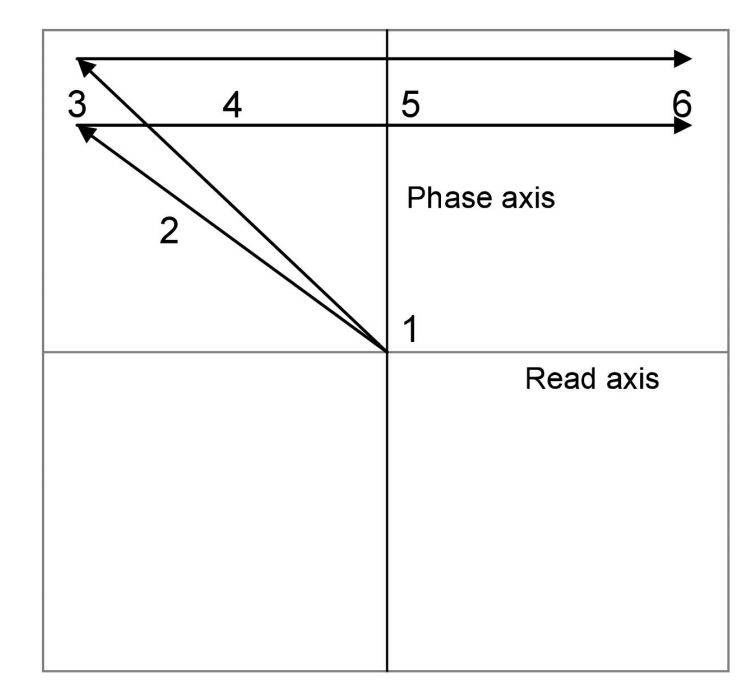
\includegraphics[width = 0.5\textwidth]{Abbildungen/2DMRI.JPG}
    \caption[Veranschaulichter Verlauf des k-Vektors im 2D-MRI]{Hier wird anschaulich ein Verlauf des k-Vektors in der transversalen Ebene dargestellt.\\
    Als Erster wird in Schritt 1 das Signal durch den $90^{\circ}$-Puls in die transversalen Ebene gebracht.\\
    Anschließend wird ein Gradient in negativer \textit{read}-Richtung eingeschaltet. Zusätzlich wird auch der Phasengradient $G_p$ angelegt. Dies bedeutet, dass der k-Vektor in Abhängigkeit von der Zeit durch den \textit{phasen}-und \textit{read}-Raum durchgeht. Dies ist in der Abbildung mit der Nummer 2 markiert, wo der Pfeil vom Ursprung quer nach links oben verläuft.\\
    Im dritten Schritt wird der Phasengradient ausgeschaltet was bedeutet, dass sich der k-Vektor nicht mehr entlang des Phasenraums bewegt und somit nur noch von dem Gradienten in der \textit{read}-Richtung abhängt. Das Vorzeichen von dem \textit{read}-Gradienten wird geflippt, sodass dieser nicht mehr negativ ist sondern positiv. Ab hier findet nun der gleiche Ablauf wie bei der 1D-MRI-Messung statt. Die Larmorfrequenz der Spins werden in Abhängigkeit von der Position gemessen, sodass am Ende eine Linie von Datenpunkte heraus kommt. Diese wurden  zusätzlich noch in Abhängigkeit von der Zeit gemessen. Nachdem eine Linie im k-Raum vermessen wurde, wird der Gradient ausgeschaltet und dieser fängt wieder vom Anfang an.\\ \cite{Schmidt}}
    \label{fig:2DMRIk}
\end{figure}
Durch das Wiederholen der in Abbildung \ref{fig:2DMRIk} dargestellten Messmethode ergibt dies am Ende ein 2D-MRI. Vereinfacht gesagt, ist ein 2D-MRI ein 1D-MRI, welches durch sehr viele Ebenen durchgefahren wurde.

Das Ziel bei dem 2D-MRI ist es nun, welche Auswirkungen unterschiedliche Relaxationszeiten von $T_1$ und $T_2$ auf die Messungen haben und wie diese Kontraste erhöht werden können. Durch Kontrastmittel können unter anderem die Relaxationszeiten der zu untersuchenden Proben verändert werden. Hierbei wird zwischen positiven Relaxationszeiten (diese erhöhen die Intensität der Probe) und negative Kontraste ( diese verringern/reduziert die Intensität in der Region) unterschieden.  Diese Kontrastmittel werden dann benutzt, wenn in einer bestimmten Region etwas hervor gehoben werden soll oder schon einen vorhanden Kontrast weiter verstärkt werden soll. \\
Diese Kontrastmittel sind vor allem in der Medizin von großer Bedeutung. Die Kontrastmittel können hierbei von den Patienten Oral eingenommen werden oder werden direkt in die Region gespritz, die von Interesse sind.   
\begin{figure}[H]
\centering
\subcaptionbox{Die Polarisationszeit von $\SI{600}{\milli\second}$ wurde am Anfang gewählt. Dabei handelt es sich um die selbe Zeit wie die $T_1$-Relaxation von der einen Röhre. Hierbei ist in der Abbildung zu sehen, dass es sich um die rechte Röhre handeln muss, da diese bei geringer Polarisationszeit schon eine sehr große Intensität aufweist}
{% GNUPLOT: LaTeX picture with Postscript
\begingroup
  % Encoding inside the plot.  In the header of your document, this encoding
  % should to defined, e.g., by using
  % \usepackage[cp1252,<other encodings>]{inputenc}
  \inputencoding{cp1252}%
  \makeatletter
  \providecommand\color[2][]{%
    \GenericError{(gnuplot) \space\space\space\@spaces}{%
      Package color not loaded in conjunction with
      terminal option `colourtext'%
    }{See the gnuplot documentation for explanation.%
    }{Either use 'blacktext' in gnuplot or load the package
      color.sty in LaTeX.}%
    \renewcommand\color[2][]{}%
  }%
  \providecommand\includegraphics[2][]{%
    \GenericError{(gnuplot) \space\space\space\@spaces}{%
      Package graphicx or graphics not loaded%
    }{See the gnuplot documentation for explanation.%
    }{The gnuplot epslatex terminal needs graphicx.sty or graphics.sty.}%
    \renewcommand\includegraphics[2][]{}%
  }%
  \providecommand\rotatebox[2]{#2}%
  \@ifundefined{ifGPcolor}{%
    \newif\ifGPcolor
    \GPcolorfalse
  }{}%
  \@ifundefined{ifGPblacktext}{%
    \newif\ifGPblacktext
    \GPblacktexttrue
  }{}%
  % define a \g@addto@macro without @ in the name:
  \let\gplgaddtomacro\g@addto@macro
  % define empty templates for all commands taking text:
  \gdef\gplbacktext{}%
  \gdef\gplfronttext{}%
  \makeatother
  \ifGPblacktext
    % no textcolor at all
    \def\colorrgb#1{}%
    \def\colorgray#1{}%
  \else
    % gray or color?
    \ifGPcolor
      \def\colorrgb#1{\color[rgb]{#1}}%
      \def\colorgray#1{\color[gray]{#1}}%
      \expandafter\def\csname LTw\endcsname{\color{white}}%
      \expandafter\def\csname LTb\endcsname{\color{black}}%
      \expandafter\def\csname LTa\endcsname{\color{black}}%
      \expandafter\def\csname LT0\endcsname{\color[rgb]{1,0,0}}%
      \expandafter\def\csname LT1\endcsname{\color[rgb]{0,1,0}}%
      \expandafter\def\csname LT2\endcsname{\color[rgb]{0,0,1}}%
      \expandafter\def\csname LT3\endcsname{\color[rgb]{1,0,1}}%
      \expandafter\def\csname LT4\endcsname{\color[rgb]{0,1,1}}%
      \expandafter\def\csname LT5\endcsname{\color[rgb]{1,1,0}}%
      \expandafter\def\csname LT6\endcsname{\color[rgb]{0,0,0}}%
      \expandafter\def\csname LT7\endcsname{\color[rgb]{1,0.3,0}}%
      \expandafter\def\csname LT8\endcsname{\color[rgb]{0.5,0.5,0.5}}%
    \else
      % gray
      \def\colorrgb#1{\color{black}}%
      \def\colorgray#1{\color[gray]{#1}}%
      \expandafter\def\csname LTw\endcsname{\color{white}}%
      \expandafter\def\csname LTb\endcsname{\color{black}}%
      \expandafter\def\csname LTa\endcsname{\color{black}}%
      \expandafter\def\csname LT0\endcsname{\color{black}}%
      \expandafter\def\csname LT1\endcsname{\color{black}}%
      \expandafter\def\csname LT2\endcsname{\color{black}}%
      \expandafter\def\csname LT3\endcsname{\color{black}}%
      \expandafter\def\csname LT4\endcsname{\color{black}}%
      \expandafter\def\csname LT5\endcsname{\color{black}}%
      \expandafter\def\csname LT6\endcsname{\color{black}}%
      \expandafter\def\csname LT7\endcsname{\color{black}}%
      \expandafter\def\csname LT8\endcsname{\color{black}}%
    \fi
  \fi
    \setlength{\unitlength}{0.0500bp}%
    \ifx\gptboxheight\undefined%
      \newlength{\gptboxheight}%
      \newlength{\gptboxwidth}%
      \newsavebox{\gptboxtext}%
    \fi%
    \setlength{\fboxrule}{0.5pt}%
    \setlength{\fboxsep}{1pt}%
\begin{picture}(7200.00,5040.00)%
    \gplgaddtomacro\gplbacktext{%
    }%
    \gplgaddtomacro\gplfronttext{%
      \csname LTb\endcsname%%
      \put(936,688){\makebox(0,0){\strut{}$0$}}%
      \put(1824,688){\makebox(0,0){\strut{}$20$}}%
      \put(2712,688){\makebox(0,0){\strut{}$40$}}%
      \put(3600,688){\makebox(0,0){\strut{}$60$}}%
      \put(4488,688){\makebox(0,0){\strut{}$80$}}%
      \put(5376,688){\makebox(0,0){\strut{}$100$}}%
      \put(6264,688){\makebox(0,0){\strut{}$120$}}%
      \put(3600,358){\makebox(0,0){\strut{}Y in $\si{\milli \meter}$}}%
      \put(700,938){\makebox(0,0)[r]{\strut{}$0$}}%
      \put(700,1502){\makebox(0,0)[r]{\strut{}$20$}}%
      \put(700,2066){\makebox(0,0)[r]{\strut{}$40$}}%
      \put(700,2630){\makebox(0,0)[r]{\strut{}$60$}}%
      \put(700,3194){\makebox(0,0)[r]{\strut{}$80$}}%
      \put(700,3758){\makebox(0,0)[r]{\strut{}$100$}}%
      \put(700,4322){\makebox(0,0)[r]{\strut{}$120$}}%
      \put(238,2630){\rotatebox{-270}{\makebox(0,0){\strut{}Z in $\si{\milli \meter}$}}}%
      \put(6795,938){\makebox(0,0)[l]{\strut{}$0$}}%
      \put(6795,1421){\makebox(0,0)[l]{\strut{}$5000$}}%
      \put(6795,1904){\makebox(0,0)[l]{\strut{}$10000$}}%
      \put(6795,2388){\makebox(0,0)[l]{\strut{}$15000$}}%
      \put(6795,2871){\makebox(0,0)[l]{\strut{}$20000$}}%
      \put(6795,3355){\makebox(0,0)[l]{\strut{}$25000$}}%
      \put(6795,3838){\makebox(0,0)[l]{\strut{}$30000$}}%
      \put(6795,4322){\makebox(0,0)[l]{\strut{}$35000$}}%
    }%
    \gplbacktext
    \put(0,0){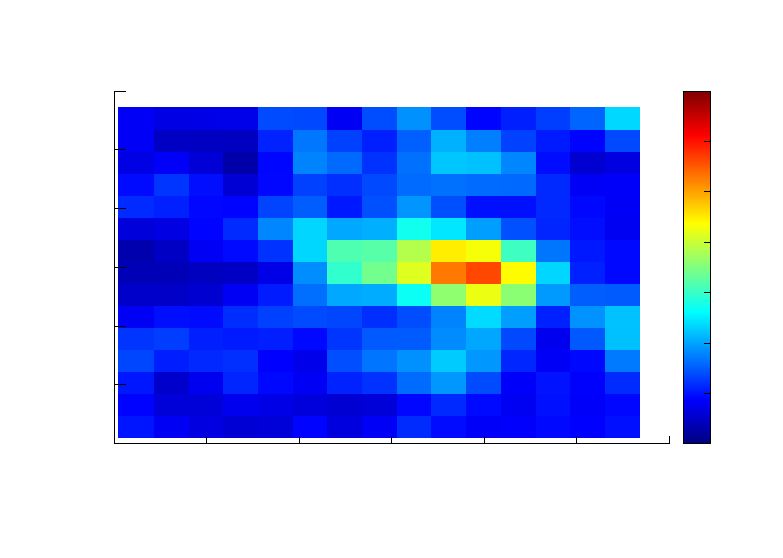
\includegraphics{plots/2DMRI600}}%
    \gplfronttext
  \end{picture}%
\endgroup
}
% \subcaptionbox{Es wurde als nächstes eine Polarisationszeit von $\SI{1300}{\milli\second}$ gewählt, wobei es sich hierbei um einen Wert zwischen den beiden Polarisationszeiten handelt.}
% {% GNUPLOT: LaTeX picture with Postscript
\begingroup
  % Encoding inside the plot.  In the header of your document, this encoding
  % should to defined, e.g., by using
  % \usepackage[cp1252,<other encodings>]{inputenc}
  \inputencoding{cp1252}%
  \makeatletter
  \providecommand\color[2][]{%
    \GenericError{(gnuplot) \space\space\space\@spaces}{%
      Package color not loaded in conjunction with
      terminal option `colourtext'%
    }{See the gnuplot documentation for explanation.%
    }{Either use 'blacktext' in gnuplot or load the package
      color.sty in LaTeX.}%
    \renewcommand\color[2][]{}%
  }%
  \providecommand\includegraphics[2][]{%
    \GenericError{(gnuplot) \space\space\space\@spaces}{%
      Package graphicx or graphics not loaded%
    }{See the gnuplot documentation for explanation.%
    }{The gnuplot epslatex terminal needs graphicx.sty or graphics.sty.}%
    \renewcommand\includegraphics[2][]{}%
  }%
  \providecommand\rotatebox[2]{#2}%
  \@ifundefined{ifGPcolor}{%
    \newif\ifGPcolor
    \GPcolorfalse
  }{}%
  \@ifundefined{ifGPblacktext}{%
    \newif\ifGPblacktext
    \GPblacktexttrue
  }{}%
  % define a \g@addto@macro without @ in the name:
  \let\gplgaddtomacro\g@addto@macro
  % define empty templates for all commands taking text:
  \gdef\gplbacktext{}%
  \gdef\gplfronttext{}%
  \makeatother
  \ifGPblacktext
    % no textcolor at all
    \def\colorrgb#1{}%
    \def\colorgray#1{}%
  \else
    % gray or color?
    \ifGPcolor
      \def\colorrgb#1{\color[rgb]{#1}}%
      \def\colorgray#1{\color[gray]{#1}}%
      \expandafter\def\csname LTw\endcsname{\color{white}}%
      \expandafter\def\csname LTb\endcsname{\color{black}}%
      \expandafter\def\csname LTa\endcsname{\color{black}}%
      \expandafter\def\csname LT0\endcsname{\color[rgb]{1,0,0}}%
      \expandafter\def\csname LT1\endcsname{\color[rgb]{0,1,0}}%
      \expandafter\def\csname LT2\endcsname{\color[rgb]{0,0,1}}%
      \expandafter\def\csname LT3\endcsname{\color[rgb]{1,0,1}}%
      \expandafter\def\csname LT4\endcsname{\color[rgb]{0,1,1}}%
      \expandafter\def\csname LT5\endcsname{\color[rgb]{1,1,0}}%
      \expandafter\def\csname LT6\endcsname{\color[rgb]{0,0,0}}%
      \expandafter\def\csname LT7\endcsname{\color[rgb]{1,0.3,0}}%
      \expandafter\def\csname LT8\endcsname{\color[rgb]{0.5,0.5,0.5}}%
    \else
      % gray
      \def\colorrgb#1{\color{black}}%
      \def\colorgray#1{\color[gray]{#1}}%
      \expandafter\def\csname LTw\endcsname{\color{white}}%
      \expandafter\def\csname LTb\endcsname{\color{black}}%
      \expandafter\def\csname LTa\endcsname{\color{black}}%
      \expandafter\def\csname LT0\endcsname{\color{black}}%
      \expandafter\def\csname LT1\endcsname{\color{black}}%
      \expandafter\def\csname LT2\endcsname{\color{black}}%
      \expandafter\def\csname LT3\endcsname{\color{black}}%
      \expandafter\def\csname LT4\endcsname{\color{black}}%
      \expandafter\def\csname LT5\endcsname{\color{black}}%
      \expandafter\def\csname LT6\endcsname{\color{black}}%
      \expandafter\def\csname LT7\endcsname{\color{black}}%
      \expandafter\def\csname LT8\endcsname{\color{black}}%
    \fi
  \fi
    \setlength{\unitlength}{0.0500bp}%
    \ifx\gptboxheight\undefined%
      \newlength{\gptboxheight}%
      \newlength{\gptboxwidth}%
      \newsavebox{\gptboxtext}%
    \fi%
    \setlength{\fboxrule}{0.5pt}%
    \setlength{\fboxsep}{1pt}%
\begin{picture}(7200.00,5040.00)%
    \gplgaddtomacro\gplbacktext{%
    }%
    \gplgaddtomacro\gplfronttext{%
      \csname LTb\endcsname%%
      \put(936,688){\makebox(0,0){\strut{}$0$}}%
      \put(1824,688){\makebox(0,0){\strut{}$20$}}%
      \put(2712,688){\makebox(0,0){\strut{}$40$}}%
      \put(3600,688){\makebox(0,0){\strut{}$60$}}%
      \put(4488,688){\makebox(0,0){\strut{}$80$}}%
      \put(5376,688){\makebox(0,0){\strut{}$100$}}%
      \put(6264,688){\makebox(0,0){\strut{}$120$}}%
      \put(3600,358){\makebox(0,0){\strut{}Y in $\si{\milli \meter}$}}%
      \put(700,938){\makebox(0,0)[r]{\strut{}$0$}}%
      \put(700,1502){\makebox(0,0)[r]{\strut{}$20$}}%
      \put(700,2066){\makebox(0,0)[r]{\strut{}$40$}}%
      \put(700,2630){\makebox(0,0)[r]{\strut{}$60$}}%
      \put(700,3194){\makebox(0,0)[r]{\strut{}$80$}}%
      \put(700,3758){\makebox(0,0)[r]{\strut{}$100$}}%
      \put(700,4322){\makebox(0,0)[r]{\strut{}$120$}}%
      \put(238,2630){\rotatebox{-270}{\makebox(0,0){\strut{}Z in $\si{\milli \meter}$}}}%
      \put(6795,938){\makebox(0,0)[l]{\strut{}$0$}}%
      \put(6795,1502){\makebox(0,0)[l]{\strut{}$10000$}}%
      \put(6795,2066){\makebox(0,0)[l]{\strut{}$20000$}}%
      \put(6795,2630){\makebox(0,0)[l]{\strut{}$30000$}}%
      \put(6795,3194){\makebox(0,0)[l]{\strut{}$40000$}}%
      \put(6795,3758){\makebox(0,0)[l]{\strut{}$50000$}}%
      \put(6795,4322){\makebox(0,0)[l]{\strut{}$60000$}}%
    }%
    \gplbacktext
    \put(0,0){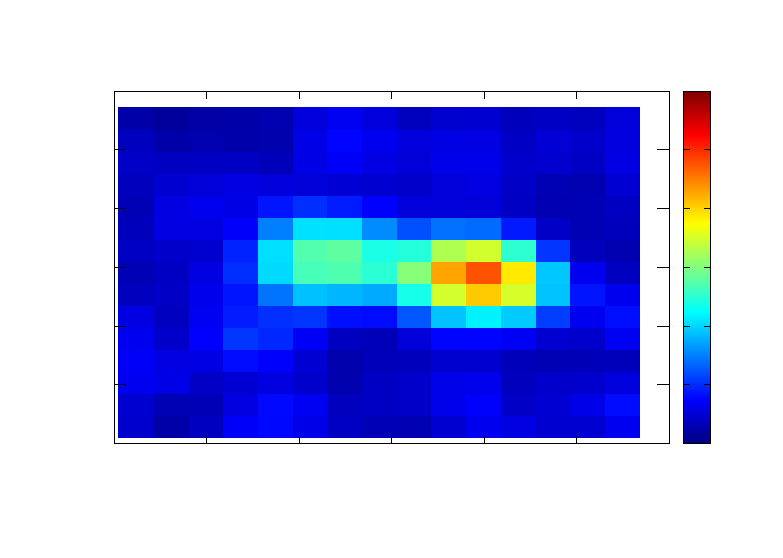
\includegraphics{plots/2DMRI1300}}%
    \gplfronttext
  \end{picture}%
\endgroup
}\newpage
\subcaptionbox{Im letzten Bild sollte eine Polarisationszeit doppelt so lange wie die längere $T_1$-Relaxation gewählt werden. Es wurde jedoch nur eine Polarisationszeit von $\SI{2800}{\milli\second}$ gemessen. Dabei handelt es sich um ca. das 1,5-fache der $T_1$-Zeit von der linken Röhre.}
{% GNUPLOT: LaTeX picture with Postscript
\begingroup
  % Encoding inside the plot.  In the header of your document, this encoding
  % should to defined, e.g., by using
  % \usepackage[cp1252,<other encodings>]{inputenc}
  \inputencoding{cp1252}%
  \makeatletter
  \providecommand\color[2][]{%
    \GenericError{(gnuplot) \space\space\space\@spaces}{%
      Package color not loaded in conjunction with
      terminal option `colourtext'%
    }{See the gnuplot documentation for explanation.%
    }{Either use 'blacktext' in gnuplot or load the package
      color.sty in LaTeX.}%
    \renewcommand\color[2][]{}%
  }%
  \providecommand\includegraphics[2][]{%
    \GenericError{(gnuplot) \space\space\space\@spaces}{%
      Package graphicx or graphics not loaded%
    }{See the gnuplot documentation for explanation.%
    }{The gnuplot epslatex terminal needs graphicx.sty or graphics.sty.}%
    \renewcommand\includegraphics[2][]{}%
  }%
  \providecommand\rotatebox[2]{#2}%
  \@ifundefined{ifGPcolor}{%
    \newif\ifGPcolor
    \GPcolorfalse
  }{}%
  \@ifundefined{ifGPblacktext}{%
    \newif\ifGPblacktext
    \GPblacktexttrue
  }{}%
  % define a \g@addto@macro without @ in the name:
  \let\gplgaddtomacro\g@addto@macro
  % define empty templates for all commands taking text:
  \gdef\gplbacktext{}%
  \gdef\gplfronttext{}%
  \makeatother
  \ifGPblacktext
    % no textcolor at all
    \def\colorrgb#1{}%
    \def\colorgray#1{}%
  \else
    % gray or color?
    \ifGPcolor
      \def\colorrgb#1{\color[rgb]{#1}}%
      \def\colorgray#1{\color[gray]{#1}}%
      \expandafter\def\csname LTw\endcsname{\color{white}}%
      \expandafter\def\csname LTb\endcsname{\color{black}}%
      \expandafter\def\csname LTa\endcsname{\color{black}}%
      \expandafter\def\csname LT0\endcsname{\color[rgb]{1,0,0}}%
      \expandafter\def\csname LT1\endcsname{\color[rgb]{0,1,0}}%
      \expandafter\def\csname LT2\endcsname{\color[rgb]{0,0,1}}%
      \expandafter\def\csname LT3\endcsname{\color[rgb]{1,0,1}}%
      \expandafter\def\csname LT4\endcsname{\color[rgb]{0,1,1}}%
      \expandafter\def\csname LT5\endcsname{\color[rgb]{1,1,0}}%
      \expandafter\def\csname LT6\endcsname{\color[rgb]{0,0,0}}%
      \expandafter\def\csname LT7\endcsname{\color[rgb]{1,0.3,0}}%
      \expandafter\def\csname LT8\endcsname{\color[rgb]{0.5,0.5,0.5}}%
    \else
      % gray
      \def\colorrgb#1{\color{black}}%
      \def\colorgray#1{\color[gray]{#1}}%
      \expandafter\def\csname LTw\endcsname{\color{white}}%
      \expandafter\def\csname LTb\endcsname{\color{black}}%
      \expandafter\def\csname LTa\endcsname{\color{black}}%
      \expandafter\def\csname LT0\endcsname{\color{black}}%
      \expandafter\def\csname LT1\endcsname{\color{black}}%
      \expandafter\def\csname LT2\endcsname{\color{black}}%
      \expandafter\def\csname LT3\endcsname{\color{black}}%
      \expandafter\def\csname LT4\endcsname{\color{black}}%
      \expandafter\def\csname LT5\endcsname{\color{black}}%
      \expandafter\def\csname LT6\endcsname{\color{black}}%
      \expandafter\def\csname LT7\endcsname{\color{black}}%
      \expandafter\def\csname LT8\endcsname{\color{black}}%
    \fi
  \fi
    \setlength{\unitlength}{0.0500bp}%
    \ifx\gptboxheight\undefined%
      \newlength{\gptboxheight}%
      \newlength{\gptboxwidth}%
      \newsavebox{\gptboxtext}%
    \fi%
    \setlength{\fboxrule}{0.5pt}%
    \setlength{\fboxsep}{1pt}%
\begin{picture}(7200.00,5040.00)%
    \gplgaddtomacro\gplbacktext{%
    }%
    \gplgaddtomacro\gplfronttext{%
      \csname LTb\endcsname%%
      \put(936,688){\makebox(0,0){\strut{}$0$}}%
      \put(1824,688){\makebox(0,0){\strut{}$20$}}%
      \put(2712,688){\makebox(0,0){\strut{}$40$}}%
      \put(3600,688){\makebox(0,0){\strut{}$60$}}%
      \put(4488,688){\makebox(0,0){\strut{}$80$}}%
      \put(5376,688){\makebox(0,0){\strut{}$100$}}%
      \put(6264,688){\makebox(0,0){\strut{}$120$}}%
      \put(3600,358){\makebox(0,0){\strut{}Y in $\si{\milli \meter}$}}%
      \put(700,938){\makebox(0,0)[r]{\strut{}$0$}}%
      \put(700,1502){\makebox(0,0)[r]{\strut{}$20$}}%
      \put(700,2066){\makebox(0,0)[r]{\strut{}$40$}}%
      \put(700,2630){\makebox(0,0)[r]{\strut{}$60$}}%
      \put(700,3194){\makebox(0,0)[r]{\strut{}$80$}}%
      \put(700,3758){\makebox(0,0)[r]{\strut{}$100$}}%
      \put(700,4322){\makebox(0,0)[r]{\strut{}$120$}}%
      \put(238,2630){\rotatebox{-270}{\makebox(0,0){\strut{}Z in $\si{\milli \meter}$}}}%
      \put(6795,938){\makebox(0,0)[l]{\strut{}$0$}}%
      \put(6795,1502){\makebox(0,0)[l]{\strut{}$10000$}}%
      \put(6795,2066){\makebox(0,0)[l]{\strut{}$20000$}}%
      \put(6795,2630){\makebox(0,0)[l]{\strut{}$30000$}}%
      \put(6795,3194){\makebox(0,0)[l]{\strut{}$40000$}}%
      \put(6795,3758){\makebox(0,0)[l]{\strut{}$50000$}}%
      \put(6795,4322){\makebox(0,0)[l]{\strut{}$60000$}}%
    }%
    \gplbacktext
    \put(0,0){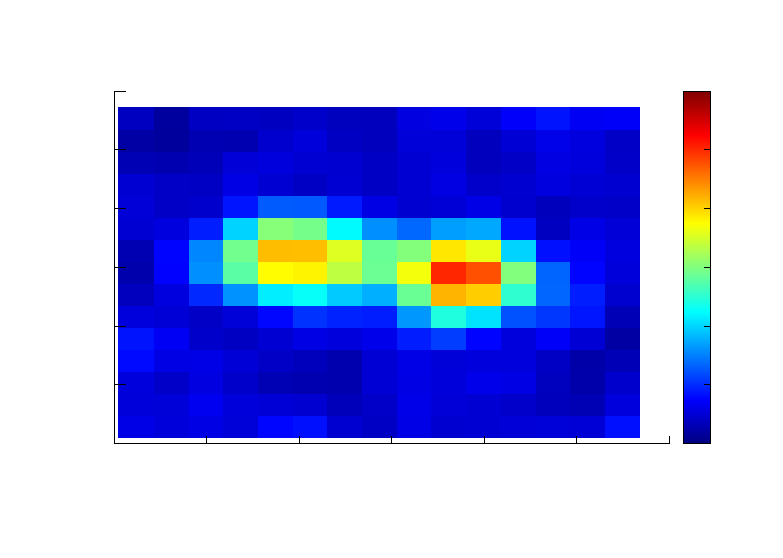
\includegraphics{plots/2DMRI2800}}%
    \gplfronttext
  \end{picture}%
\endgroup
}
\caption[Kontraste von $T_1$-Relaxation werden deutlich gemacht indem die Polarisationszeiten verändert werden]{Kontraste von $T_1$-Relaxation werden deutlich gemacht indem die Polarisationszeiten verändert werden. In Abb. (a) ist deutlich zu sehen, dass die Intensität rechts im Bild sehr groß ist. Hierbei kann auf eine kurze $T_1$-Zeit geschlossen werden, da die Spins sich in der rechten Röhre schon angefangen haben auszurichten und somit zum Signal beitragen. Bei längeren Polarisationszeiten ist zu erkennen, dass auch die Spins in der linken Röhre sich ausgerichtet haben und somit auch hier ein Signal detektiert werden kann. }\label{fig:11600}
\end{figure}
In der Abbildung \ref{fig:11600} wird eine Polarisationszeit von $\SI{600}{\milli\second}$ verwendet,
 welches die kürzere $T_1$-Zeit von der einen Röhre darstellt. Diese Röhre kann in Abb. \ref{fig:11600} unter anderem dadurch beobachtet werden,
dass sie durch eine starke Intensität dargestellt wird. Da diese Farbe von dem Rest hervorgehoben wird, wird dies als positives Kontrastmittel bezeichnet.
Die Intensitätsskalierung rechts von der Abbildung ist eine vom Programm kodierte Größe, die keine Einheit besitzt.\\

Warum die eine Röhre intensiver leuchtet als die andere, liegt am Zusammenhang zwischen der Polarisationszeit und der $T_1$-Relaxation. Die $T_1$-Relaxation gibt die Zeit an, bei der die meisten Spins sich dem äußeren Magnetfeld angepasst haben. Dies bedeutet, je kürzer $T_1$ ist, desto kürzer muss der Polarisationspuls sein um die meisten Spins im Material auszurichten. Wenn nun weiter gedacht wird und ein Material mit zwei $T_1$-Zeiten zur Untersuchung bereit stehen hat, so ist bei kleiner Polarisationszeit genau der Teil im Bild intensiver zu sehen, der eine kleinere $T_1$-Zeit besitzt, da in diesem Teil die meisten Spins sich schon ausgerichtet haben und dementsprechend zu dem MRI Signal beitragen können.\\
Durch Erhöhung der Polarisationszeit kann unteranderem auch die zweite Röhre sichtbar gemacht werden. Diese wird unter anderem in der Abb \ref{fig:11600} (b)  deutlich gemacht. Neben der Röhre die rechts unten im Bild vorhanden ist, ist hier auch die andere Röhre mit der größerer $T_1$-Zeit zu sehen. Hierbei sollte eine Polarisationszeit doppelt so groß wie die größere $T_1$ Zeit genommen werden, da in beiden Materialien versucht wird die ganzen Spins auszurichten. Am Versuchstag wurde sich mit einer Zeit von $\SI{2800}{\milli\second}$ zufrieden gegeben, da diese ausreichend zeigt, dass nun auch die zweite Röhre zu dem signal beiträgt. Dennoch ist ein Kontrast zwischen den beiden Bildern zu sehen. Dies lässt darauf schließen, dass in der Röhre links in der Abbildung insgesamt weniger Spins vorhanden sind, die zu dem Signal beitragen und somit auch logischerweise die Intensität geringer ist. Womöglich ist ein anderer Grund, dass die Polarisationszeit nicht lange genug gewählt wurde, sodass hier nicht alle Spins ausgerichtet waren. Jedoch ist offensichtlich ein Unterschied zwischen den beiden Bildern sichtbar, welcher auch erklärt werden kann. Dies ist bei einer qualitativen Beobachtung das Wichtigste und somit genügen die zwei Abbildungen als Vergleich. Wenn zusätzlich noch eine Messung mit einer Polarisationszeit betrachtet wird, die sich zwischen den zwei $T_1$ Zeiten befindet, so müsste ein Teil von der einen Röhre schon sichtbar sein, jedoch dürfte die Intensität dieser Röhre geringer sein und somit einen bläulicheren Ton besitzten. Mit der Polarisationszeit von $\SI{1300}{\milli\second}$ wurde genau so eine Messung durchgeführt und in Abb \ref{fig: 1300} kann genau diese Vermutung beobachtet werden.
    \begin{figure}[H]
        \centering
        % GNUPLOT: LaTeX picture with Postscript
\begingroup
  % Encoding inside the plot.  In the header of your document, this encoding
  % should to defined, e.g., by using
  % \usepackage[cp1252,<other encodings>]{inputenc}
  \inputencoding{cp1252}%
  \makeatletter
  \providecommand\color[2][]{%
    \GenericError{(gnuplot) \space\space\space\@spaces}{%
      Package color not loaded in conjunction with
      terminal option `colourtext'%
    }{See the gnuplot documentation for explanation.%
    }{Either use 'blacktext' in gnuplot or load the package
      color.sty in LaTeX.}%
    \renewcommand\color[2][]{}%
  }%
  \providecommand\includegraphics[2][]{%
    \GenericError{(gnuplot) \space\space\space\@spaces}{%
      Package graphicx or graphics not loaded%
    }{See the gnuplot documentation for explanation.%
    }{The gnuplot epslatex terminal needs graphicx.sty or graphics.sty.}%
    \renewcommand\includegraphics[2][]{}%
  }%
  \providecommand\rotatebox[2]{#2}%
  \@ifundefined{ifGPcolor}{%
    \newif\ifGPcolor
    \GPcolorfalse
  }{}%
  \@ifundefined{ifGPblacktext}{%
    \newif\ifGPblacktext
    \GPblacktexttrue
  }{}%
  % define a \g@addto@macro without @ in the name:
  \let\gplgaddtomacro\g@addto@macro
  % define empty templates for all commands taking text:
  \gdef\gplbacktext{}%
  \gdef\gplfronttext{}%
  \makeatother
  \ifGPblacktext
    % no textcolor at all
    \def\colorrgb#1{}%
    \def\colorgray#1{}%
  \else
    % gray or color?
    \ifGPcolor
      \def\colorrgb#1{\color[rgb]{#1}}%
      \def\colorgray#1{\color[gray]{#1}}%
      \expandafter\def\csname LTw\endcsname{\color{white}}%
      \expandafter\def\csname LTb\endcsname{\color{black}}%
      \expandafter\def\csname LTa\endcsname{\color{black}}%
      \expandafter\def\csname LT0\endcsname{\color[rgb]{1,0,0}}%
      \expandafter\def\csname LT1\endcsname{\color[rgb]{0,1,0}}%
      \expandafter\def\csname LT2\endcsname{\color[rgb]{0,0,1}}%
      \expandafter\def\csname LT3\endcsname{\color[rgb]{1,0,1}}%
      \expandafter\def\csname LT4\endcsname{\color[rgb]{0,1,1}}%
      \expandafter\def\csname LT5\endcsname{\color[rgb]{1,1,0}}%
      \expandafter\def\csname LT6\endcsname{\color[rgb]{0,0,0}}%
      \expandafter\def\csname LT7\endcsname{\color[rgb]{1,0.3,0}}%
      \expandafter\def\csname LT8\endcsname{\color[rgb]{0.5,0.5,0.5}}%
    \else
      % gray
      \def\colorrgb#1{\color{black}}%
      \def\colorgray#1{\color[gray]{#1}}%
      \expandafter\def\csname LTw\endcsname{\color{white}}%
      \expandafter\def\csname LTb\endcsname{\color{black}}%
      \expandafter\def\csname LTa\endcsname{\color{black}}%
      \expandafter\def\csname LT0\endcsname{\color{black}}%
      \expandafter\def\csname LT1\endcsname{\color{black}}%
      \expandafter\def\csname LT2\endcsname{\color{black}}%
      \expandafter\def\csname LT3\endcsname{\color{black}}%
      \expandafter\def\csname LT4\endcsname{\color{black}}%
      \expandafter\def\csname LT5\endcsname{\color{black}}%
      \expandafter\def\csname LT6\endcsname{\color{black}}%
      \expandafter\def\csname LT7\endcsname{\color{black}}%
      \expandafter\def\csname LT8\endcsname{\color{black}}%
    \fi
  \fi
    \setlength{\unitlength}{0.0500bp}%
    \ifx\gptboxheight\undefined%
      \newlength{\gptboxheight}%
      \newlength{\gptboxwidth}%
      \newsavebox{\gptboxtext}%
    \fi%
    \setlength{\fboxrule}{0.5pt}%
    \setlength{\fboxsep}{1pt}%
\begin{picture}(7200.00,5040.00)%
    \gplgaddtomacro\gplbacktext{%
    }%
    \gplgaddtomacro\gplfronttext{%
      \csname LTb\endcsname%%
      \put(936,688){\makebox(0,0){\strut{}$0$}}%
      \put(1824,688){\makebox(0,0){\strut{}$20$}}%
      \put(2712,688){\makebox(0,0){\strut{}$40$}}%
      \put(3600,688){\makebox(0,0){\strut{}$60$}}%
      \put(4488,688){\makebox(0,0){\strut{}$80$}}%
      \put(5376,688){\makebox(0,0){\strut{}$100$}}%
      \put(6264,688){\makebox(0,0){\strut{}$120$}}%
      \put(3600,358){\makebox(0,0){\strut{}Y in $\si{\milli \meter}$}}%
      \put(700,938){\makebox(0,0)[r]{\strut{}$0$}}%
      \put(700,1502){\makebox(0,0)[r]{\strut{}$20$}}%
      \put(700,2066){\makebox(0,0)[r]{\strut{}$40$}}%
      \put(700,2630){\makebox(0,0)[r]{\strut{}$60$}}%
      \put(700,3194){\makebox(0,0)[r]{\strut{}$80$}}%
      \put(700,3758){\makebox(0,0)[r]{\strut{}$100$}}%
      \put(700,4322){\makebox(0,0)[r]{\strut{}$120$}}%
      \put(238,2630){\rotatebox{-270}{\makebox(0,0){\strut{}Z in $\si{\milli \meter}$}}}%
      \put(6795,938){\makebox(0,0)[l]{\strut{}$0$}}%
      \put(6795,1502){\makebox(0,0)[l]{\strut{}$10000$}}%
      \put(6795,2066){\makebox(0,0)[l]{\strut{}$20000$}}%
      \put(6795,2630){\makebox(0,0)[l]{\strut{}$30000$}}%
      \put(6795,3194){\makebox(0,0)[l]{\strut{}$40000$}}%
      \put(6795,3758){\makebox(0,0)[l]{\strut{}$50000$}}%
      \put(6795,4322){\makebox(0,0)[l]{\strut{}$60000$}}%
    }%
    \gplbacktext
    \put(0,0){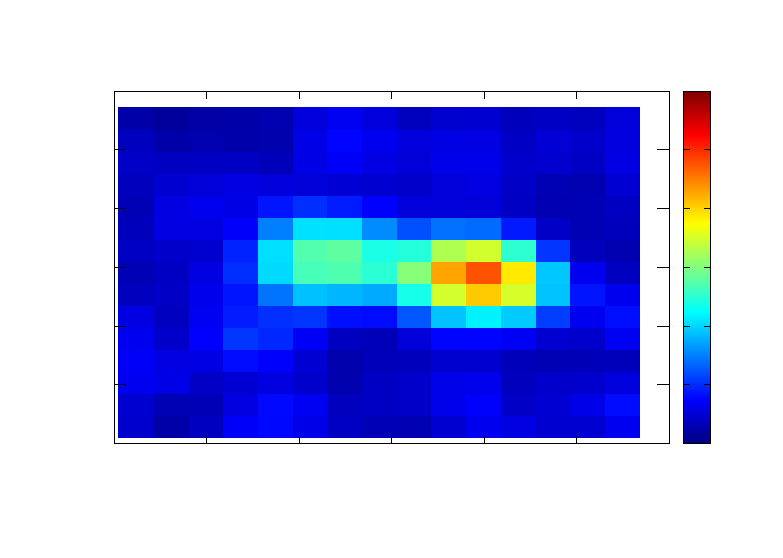
\includegraphics{plots/2DMRI1300}}%
    \gplfronttext
  \end{picture}%
\endgroup

        \caption[2D MRI mit der Polarisationszeit $\SI{1300}{\milli\second}$]{2D MRI mit der Polarisationszeit $\SI{1300}{\milli\second}$. Wie zu erwarten ist, ist das Signal in der linken Röhre noch nicht so intensiv wie in Abb. \ref{fig:11600} (b). Dies lässt sich dadurch erklären, dass die Polarisationszeit nicht komplett ausreicht um alle Spins schon aus zu richten, jedoch aber einige Spins schon ausgerichtet wurden.}
        \label{fig: 1300}
    \end{figure}
Nun gibt es noch zwei verschiedene Sachen, die betrachtet werden können. Das erste was diskutiert werden muss ist, dass in der ersten Abb \ref{fig:11600} an manchen Stellen ein Signal vorhanden ist, wo keins sein dürfte. Somit wird außerhalb von dem Phantom ein Signal gemessen. Dies könnte unter anderem daran liegen, dass während des Messvorgang eine Matrixgröße von 64$\times$ 64 genommen wurde, sodass die Messzeit sehr lange gewesen ist. Diese wurde jedoch abgebrochen, weil diese zu lange gedauert hat und somit sind die Messdaten nicht vollständig, bzw. könnten wie bei einer anderen Datei beschädigt sein. Wenn nicht ausreichend Messpunkte genommen worden sind, kann es sein, dass die Auflösung nicht gut genug ist und somit das Phantom verschwommener dargestellt wird, was auch eine Ursache darstellen könnte.\\
Aus den Abbildungen kann entnommen werden, dass die Substanz in der rechten Röhre eine kleinere $T_1$-Relaxation hat als die Substanz in der linken Röhre.\\
In dem Abschnitt über die \glqq Relaxationszeiten von Wasser und Zusatzmitteln\grqq \, wurden verschiedene Konzentrationen von Stoffen untersucht auf die jeweiligen Relaxationszeiten. In der ersten Abbildung \ref{fig:11600} ist schon bei einer geringen Polarisationszeit die rechte Röhre deutlich zu sehen. Dies legt die Vermutung nahe, dass die Substanz in der  rechten Röhre eine $T_1$-Zeit besitzt, die bei ca. $\SI{600}{\milli\second}$ liegt. Mit dieser Vermutung kann aus der Tabelle \ref{tab:T1T2} entnommen werden, dass es sich hierbei um \ce{Cu2+} mit einer Konzentration von $\SI{500}{\micro\mole}$ oder 
$\SI{1000}{\micro\mole}$ handelt. Um dies genau zu ermitteln, müsste vor dem 2D-MRI 
eine $T_2$ Messung stattfinden, ohne dass sich in der anderen Röhre etwas befindet. Die Konzentration von $\SI{2000}{\micro\mole}$ wurde ausgeschlossen, da die Signalintensität noch leicht ansteigt, wenn die Polarisationszeit weiter erhöht wird. Dies spricht dafür, dass die Polarisationszeit von $\SI{600}{\milli\second}$ nicht komplett ausreicht um alle Spins auszurichten. Falls es kein Kupfer ist, kann es sich möglicherweise um \ce{Mn2+} handeln mit einer Konzentration von ca. $\SI{50}{\micro\mole}$. Die Begründug hierfür wären analog wie zum Kupfer. Weitere Stoffe oder Konzentrationen können nicht genauer betrachtet werden, da es hierfür keine Referenzwerte gibt.\\
Als nächstes kann eine Vermutung angestellt werden, was sich in der linken Röhre befindet. Hierbei wird erst bei höherer Polarisationszeit sichtbar, dass das Signal intensiver wird. Das Signal ist hierbei bei der letzten Messung am intensivsten. Der Wert, der hierfür am besten passt liefert Wasser mit einer Relaxationszeit von ca. $\SI{2200}{\milli\second}$. Alle anderen $T_1$-Zeiten würden schon früher durch die lange Polarisationszeiten erreicht werden, weshalb Kupfer und Mangan ausgeschlossen werden können.\\


Bei dem 2D-MRI wurden nicht nur die $T_1$-Konstraste angeschaut, sondern auch die unterschiedlichen Kontraste der $T_2$-Relaxationen. 

    \begin{figure}[H]
        \centering
        \subcaptionbox{$t_{echo}$=$\SI{250}{\milli\second}$}
        {% GNUPLOT: LaTeX picture with Postscript
\begingroup
  % Encoding inside the plot.  In the header of your document, this encoding
  % should to defined, e.g., by using
  % \usepackage[cp1252,<other encodings>]{inputenc}
  \inputencoding{cp1252}%
  \makeatletter
  \providecommand\color[2][]{%
    \GenericError{(gnuplot) \space\space\space\@spaces}{%
      Package color not loaded in conjunction with
      terminal option `colourtext'%
    }{See the gnuplot documentation for explanation.%
    }{Either use 'blacktext' in gnuplot or load the package
      color.sty in LaTeX.}%
    \renewcommand\color[2][]{}%
  }%
  \providecommand\includegraphics[2][]{%
    \GenericError{(gnuplot) \space\space\space\@spaces}{%
      Package graphicx or graphics not loaded%
    }{See the gnuplot documentation for explanation.%
    }{The gnuplot epslatex terminal needs graphicx.sty or graphics.sty.}%
    \renewcommand\includegraphics[2][]{}%
  }%
  \providecommand\rotatebox[2]{#2}%
  \@ifundefined{ifGPcolor}{%
    \newif\ifGPcolor
    \GPcolorfalse
  }{}%
  \@ifundefined{ifGPblacktext}{%
    \newif\ifGPblacktext
    \GPblacktexttrue
  }{}%
  % define a \g@addto@macro without @ in the name:
  \let\gplgaddtomacro\g@addto@macro
  % define empty templates for all commands taking text:
  \gdef\gplbacktext{}%
  \gdef\gplfronttext{}%
  \makeatother
  \ifGPblacktext
    % no textcolor at all
    \def\colorrgb#1{}%
    \def\colorgray#1{}%
  \else
    % gray or color?
    \ifGPcolor
      \def\colorrgb#1{\color[rgb]{#1}}%
      \def\colorgray#1{\color[gray]{#1}}%
      \expandafter\def\csname LTw\endcsname{\color{white}}%
      \expandafter\def\csname LTb\endcsname{\color{black}}%
      \expandafter\def\csname LTa\endcsname{\color{black}}%
      \expandafter\def\csname LT0\endcsname{\color[rgb]{1,0,0}}%
      \expandafter\def\csname LT1\endcsname{\color[rgb]{0,1,0}}%
      \expandafter\def\csname LT2\endcsname{\color[rgb]{0,0,1}}%
      \expandafter\def\csname LT3\endcsname{\color[rgb]{1,0,1}}%
      \expandafter\def\csname LT4\endcsname{\color[rgb]{0,1,1}}%
      \expandafter\def\csname LT5\endcsname{\color[rgb]{1,1,0}}%
      \expandafter\def\csname LT6\endcsname{\color[rgb]{0,0,0}}%
      \expandafter\def\csname LT7\endcsname{\color[rgb]{1,0.3,0}}%
      \expandafter\def\csname LT8\endcsname{\color[rgb]{0.5,0.5,0.5}}%
    \else
      % gray
      \def\colorrgb#1{\color{black}}%
      \def\colorgray#1{\color[gray]{#1}}%
      \expandafter\def\csname LTw\endcsname{\color{white}}%
      \expandafter\def\csname LTb\endcsname{\color{black}}%
      \expandafter\def\csname LTa\endcsname{\color{black}}%
      \expandafter\def\csname LT0\endcsname{\color{black}}%
      \expandafter\def\csname LT1\endcsname{\color{black}}%
      \expandafter\def\csname LT2\endcsname{\color{black}}%
      \expandafter\def\csname LT3\endcsname{\color{black}}%
      \expandafter\def\csname LT4\endcsname{\color{black}}%
      \expandafter\def\csname LT5\endcsname{\color{black}}%
      \expandafter\def\csname LT6\endcsname{\color{black}}%
      \expandafter\def\csname LT7\endcsname{\color{black}}%
      \expandafter\def\csname LT8\endcsname{\color{black}}%
    \fi
  \fi
    \setlength{\unitlength}{0.0500bp}%
    \ifx\gptboxheight\undefined%
      \newlength{\gptboxheight}%
      \newlength{\gptboxwidth}%
      \newsavebox{\gptboxtext}%
    \fi%
    \setlength{\fboxrule}{0.5pt}%
    \setlength{\fboxsep}{1pt}%
\begin{picture}(7200.00,5040.00)%
    \gplgaddtomacro\gplbacktext{%
    }%
    \gplgaddtomacro\gplfronttext{%
      \csname LTb\endcsname%%
      \put(936,688){\makebox(0,0){\strut{}$0$}}%
      \put(1824,688){\makebox(0,0){\strut{}$20$}}%
      \put(2712,688){\makebox(0,0){\strut{}$40$}}%
      \put(3600,688){\makebox(0,0){\strut{}$60$}}%
      \put(4488,688){\makebox(0,0){\strut{}$80$}}%
      \put(5376,688){\makebox(0,0){\strut{}$100$}}%
      \put(6264,688){\makebox(0,0){\strut{}$120$}}%
      \put(3600,358){\makebox(0,0){\strut{}Y in $\si{\milli \meter}$}}%
      \put(700,938){\makebox(0,0)[r]{\strut{}$0$}}%
      \put(700,1502){\makebox(0,0)[r]{\strut{}$20$}}%
      \put(700,2066){\makebox(0,0)[r]{\strut{}$40$}}%
      \put(700,2630){\makebox(0,0)[r]{\strut{}$60$}}%
      \put(700,3194){\makebox(0,0)[r]{\strut{}$80$}}%
      \put(700,3758){\makebox(0,0)[r]{\strut{}$100$}}%
      \put(700,4322){\makebox(0,0)[r]{\strut{}$120$}}%
      \put(238,2630){\rotatebox{-270}{\makebox(0,0){\strut{}Z in $\si{\milli \meter}$}}}%
      \put(6795,938){\makebox(0,0)[l]{\strut{}$0$}}%
      \put(6795,1421){\makebox(0,0)[l]{\strut{}$10000$}}%
      \put(6795,1904){\makebox(0,0)[l]{\strut{}$20000$}}%
      \put(6795,2388){\makebox(0,0)[l]{\strut{}$30000$}}%
      \put(6795,2871){\makebox(0,0)[l]{\strut{}$40000$}}%
      \put(6795,3355){\makebox(0,0)[l]{\strut{}$50000$}}%
      \put(6795,3838){\makebox(0,0)[l]{\strut{}$60000$}}%
      \put(6795,4322){\makebox(0,0)[l]{\strut{}$70000$}}%
    }%
    \gplbacktext
    \put(0,0){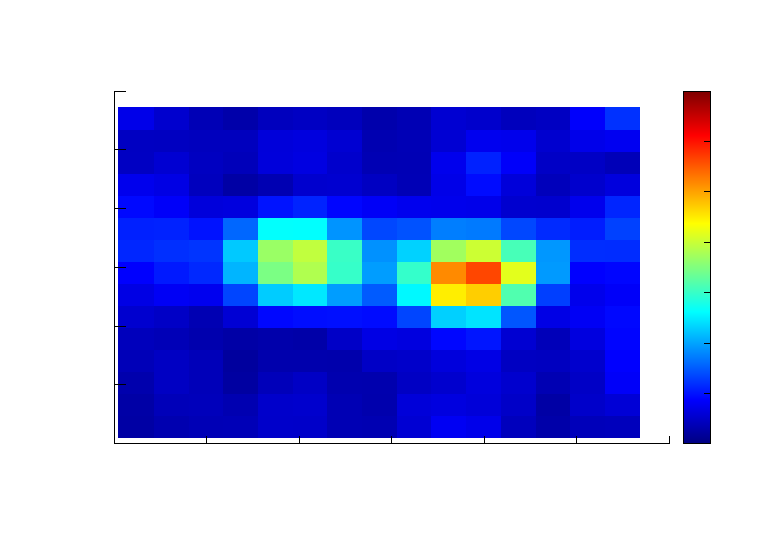
\includegraphics{plots/2DMRI250}}%
    \gplfronttext
  \end{picture}%
\endgroup
}
        \subcaptionbox{$t_{echo}$=$\SI{550}{\milli\second}$}
        {% GNUPLOT: LaTeX picture with Postscript
\begingroup
  % Encoding inside the plot.  In the header of your document, this encoding
  % should to defined, e.g., by using
  % \usepackage[cp1252,<other encodings>]{inputenc}
  \inputencoding{cp1252}%
  \makeatletter
  \providecommand\color[2][]{%
    \GenericError{(gnuplot) \space\space\space\@spaces}{%
      Package color not loaded in conjunction with
      terminal option `colourtext'%
    }{See the gnuplot documentation for explanation.%
    }{Either use 'blacktext' in gnuplot or load the package
      color.sty in LaTeX.}%
    \renewcommand\color[2][]{}%
  }%
  \providecommand\includegraphics[2][]{%
    \GenericError{(gnuplot) \space\space\space\@spaces}{%
      Package graphicx or graphics not loaded%
    }{See the gnuplot documentation for explanation.%
    }{The gnuplot epslatex terminal needs graphicx.sty or graphics.sty.}%
    \renewcommand\includegraphics[2][]{}%
  }%
  \providecommand\rotatebox[2]{#2}%
  \@ifundefined{ifGPcolor}{%
    \newif\ifGPcolor
    \GPcolorfalse
  }{}%
  \@ifundefined{ifGPblacktext}{%
    \newif\ifGPblacktext
    \GPblacktexttrue
  }{}%
  % define a \g@addto@macro without @ in the name:
  \let\gplgaddtomacro\g@addto@macro
  % define empty templates for all commands taking text:
  \gdef\gplbacktext{}%
  \gdef\gplfronttext{}%
  \makeatother
  \ifGPblacktext
    % no textcolor at all
    \def\colorrgb#1{}%
    \def\colorgray#1{}%
  \else
    % gray or color?
    \ifGPcolor
      \def\colorrgb#1{\color[rgb]{#1}}%
      \def\colorgray#1{\color[gray]{#1}}%
      \expandafter\def\csname LTw\endcsname{\color{white}}%
      \expandafter\def\csname LTb\endcsname{\color{black}}%
      \expandafter\def\csname LTa\endcsname{\color{black}}%
      \expandafter\def\csname LT0\endcsname{\color[rgb]{1,0,0}}%
      \expandafter\def\csname LT1\endcsname{\color[rgb]{0,1,0}}%
      \expandafter\def\csname LT2\endcsname{\color[rgb]{0,0,1}}%
      \expandafter\def\csname LT3\endcsname{\color[rgb]{1,0,1}}%
      \expandafter\def\csname LT4\endcsname{\color[rgb]{0,1,1}}%
      \expandafter\def\csname LT5\endcsname{\color[rgb]{1,1,0}}%
      \expandafter\def\csname LT6\endcsname{\color[rgb]{0,0,0}}%
      \expandafter\def\csname LT7\endcsname{\color[rgb]{1,0.3,0}}%
      \expandafter\def\csname LT8\endcsname{\color[rgb]{0.5,0.5,0.5}}%
    \else
      % gray
      \def\colorrgb#1{\color{black}}%
      \def\colorgray#1{\color[gray]{#1}}%
      \expandafter\def\csname LTw\endcsname{\color{white}}%
      \expandafter\def\csname LTb\endcsname{\color{black}}%
      \expandafter\def\csname LTa\endcsname{\color{black}}%
      \expandafter\def\csname LT0\endcsname{\color{black}}%
      \expandafter\def\csname LT1\endcsname{\color{black}}%
      \expandafter\def\csname LT2\endcsname{\color{black}}%
      \expandafter\def\csname LT3\endcsname{\color{black}}%
      \expandafter\def\csname LT4\endcsname{\color{black}}%
      \expandafter\def\csname LT5\endcsname{\color{black}}%
      \expandafter\def\csname LT6\endcsname{\color{black}}%
      \expandafter\def\csname LT7\endcsname{\color{black}}%
      \expandafter\def\csname LT8\endcsname{\color{black}}%
    \fi
  \fi
    \setlength{\unitlength}{0.0500bp}%
    \ifx\gptboxheight\undefined%
      \newlength{\gptboxheight}%
      \newlength{\gptboxwidth}%
      \newsavebox{\gptboxtext}%
    \fi%
    \setlength{\fboxrule}{0.5pt}%
    \setlength{\fboxsep}{1pt}%
\begin{picture}(7200.00,5040.00)%
    \gplgaddtomacro\gplbacktext{%
    }%
    \gplgaddtomacro\gplfronttext{%
      \csname LTb\endcsname%%
      \put(936,688){\makebox(0,0){\strut{}$0$}}%
      \put(1824,688){\makebox(0,0){\strut{}$20$}}%
      \put(2712,688){\makebox(0,0){\strut{}$40$}}%
      \put(3600,688){\makebox(0,0){\strut{}$60$}}%
      \put(4488,688){\makebox(0,0){\strut{}$80$}}%
      \put(5376,688){\makebox(0,0){\strut{}$100$}}%
      \put(6264,688){\makebox(0,0){\strut{}$120$}}%
      \put(3600,358){\makebox(0,0){\strut{}Y in $\si{\milli \meter}$}}%
      \put(700,938){\makebox(0,0)[r]{\strut{}$0$}}%
      \put(700,1502){\makebox(0,0)[r]{\strut{}$20$}}%
      \put(700,2066){\makebox(0,0)[r]{\strut{}$40$}}%
      \put(700,2630){\makebox(0,0)[r]{\strut{}$60$}}%
      \put(700,3194){\makebox(0,0)[r]{\strut{}$80$}}%
      \put(700,3758){\makebox(0,0)[r]{\strut{}$100$}}%
      \put(700,4322){\makebox(0,0)[r]{\strut{}$120$}}%
      \put(238,2630){\rotatebox{-270}{\makebox(0,0){\strut{}Z in $\si{\milli \meter}$}}}%
      \put(6795,938){\makebox(0,0)[l]{\strut{}$0$}}%
      \put(6795,1314){\makebox(0,0)[l]{\strut{}$5000$}}%
      \put(6795,1690){\makebox(0,0)[l]{\strut{}$10000$}}%
      \put(6795,2066){\makebox(0,0)[l]{\strut{}$15000$}}%
      \put(6795,2442){\makebox(0,0)[l]{\strut{}$20000$}}%
      \put(6795,2818){\makebox(0,0)[l]{\strut{}$25000$}}%
      \put(6795,3194){\makebox(0,0)[l]{\strut{}$30000$}}%
      \put(6795,3570){\makebox(0,0)[l]{\strut{}$35000$}}%
      \put(6795,3946){\makebox(0,0)[l]{\strut{}$40000$}}%
      \put(6795,4322){\makebox(0,0)[l]{\strut{}$45000$}}%
    }%
    \gplbacktext
    \put(0,0){\includegraphics{plots/2DMRI550}}%
    \gplfronttext
  \end{picture}%
\endgroup
}
        \caption[2D-MRI mit Relaxationskontrast von verschiedenen $T_2$-Zeiten, durch verschiedene Echozeiten]{2D-MRI mit Relaxationskontrast von verschiedenen $T_2$-Zeiten, durch verschiedene Echozeiten. Im ersten Bild (a) kann beobachtet werden, dass bei geringer Echozeit die Spins nocht nicht relaxieren konnten und das Signal noch bei beiden Röhren relativ stark ist und fast die genaue Intensität wie in \ref{fig:11600}(b) besitzten. Bei längerer Echozeit wird der Kontrast von den zwei Röhren deutlicher. Je kürzer $T_2$ ist, desto schneller verschwindet die Intensität bei längeren Echozeiten. Somit kann aus dem zweiten Bild entnommen werden, dass die linke Röhre eine längere $T_2$-Zeit hat und somitrastmittl als ein positives Kont}\label{fig:1250}
    \end{figure}
Was als erstes auffält ist, dass die Abb. \ref{fig:1250} der Abb \ref{fig:11600}  vergleichsweise sehr ähnlich aussieht. Dies liegt daran, dass bei der $T_2$-Realaxation der Kontrast mit der Zeit größer wird. (Bis zu dem Punkt wo beide keine Signale mehr besitzten) . Außerdem wurde hier auch die gleiche Polarisationszeit genommen, damit keine Unterschiede von der $T_1$-Relaxation die $T_2$-Kontraste beeinflussen. \\
Grund dafür, dass die $T_2$-Kontraste noch nicht so gut sichtbar sind liegt daran, dass bei kurzer Echozeit die Spins noch nicht stark relaxieren konnten und somit auch kein großer Unterschied im Signal vorhanden ist. Dies ändert sich jedoch mit der Messung \ref{fig:1250}, da hier das Signal von der rechten Röhre schwächer ist als in der linken Röhre. Zu beachten ist hierbei, dass die Skala sich auf der rechten Seite verändert hat und auch wenn das Signal in der linken Röhre mit rot ausgeprägt ist, dass dieses Signal leztlich auch schwächer geworden sind. Dies kann dadurch erklärt werden, dass die $T_2$-Relaxation die Zeit angibt, wie schnell ein Signal zerfällt. Dadurch, dass das Signal in der linken Röhre stärker als in der rechten Röhre zu sehen ist, handelt es sich hier um ein positives Kontrastmittel und die Substanz in der linken Röhre muss eine längere $T_2$-Relaxation besitzten.  
Dies würde auch mit der Theorie übereinstimmen, dass in der linken Röhre Wasser als Probe genommen wurde. Denn bei Wasser ist $T_2$ mit  $\SI{1901}{\milli\second}$ am größten und somit sollte das Signal auch bei längeren Echozeiten deutlicher zu sehen sein als bei Kupfer oder Mangan.
Schon in dem Kapitel davor \ref{sec:1DMRIkapitel} wurde darauf eingegangen, dass eine gute Effizienz wichtig ist, um bei einer geringen Messzeit eine gute Auflösung zu erhalten. Im zweidimensionalen wird dies um so wichtiger sein, da statt nur in eine Richtung nun eine zweite Richtung abgefahren wird, womit sich die Messzeit erheblich erhöht. Somit ist es wichtig bei dem Versuch darauf zu achten, dass die Effizienz gut ist.
% !TEX root = main.tex
\subsection{J-Kopplung zur chemischen Strukturanalyse}
Eine weitere Anwendung der NMR-Technologie stellt die Möglichkeit dar chemische Strukturen zu analysieren.
Im vorliegenden Beispiel soll dabei Difluorobenzene untersucht werden.
Dabei wird die Verbindung zum einen auf die Kopplungskostante zwischen den einzelnen Fluor- und Wasserstoffatomen analysiert, dabei kann ermittelt werden, ob schwache Kopplung vorliegt zudem sollen auch Verhältnisse der Peakgrößen betrachtet werden.
Zunächst sollen daher einige grundlegende Zusammenhänge erläutert werden.
Da es sich bei dem vorliegenden Molekül um eine hetero-nukleare Verbindung zwischen Fluor (\ce{^19F}) und Wasserstoff (\ce{^1H}) handelt und der Versuchsaufbau während des Experiments auf die Larmorfrequenz von Wasserstoff ($\omega_{\text{L,H}} = \SI{1839}{\per \second}$) ausgerichtet ist müssen zunächst justierungen vorgenommen werden.
Dabei kann nach
\begin{align}
    \omega = \gamma \cdot B , \label{eq: LarmorB}    
\end{align}
die Larmorfrequenz für Fluor ($\omega_{\text{L,F}} = \SI{1730}{\per \second}$) berechnet werden. 
Die gyromagnetischen Verhältnisse $\gamma$ von Wasserstoff ($\gamma = \SI{2.675 e8}{\per \second \per \tesla}$) und Fluor ($\gamma = \SI{2.517 e8}{\per \second \per \tesla}$) wurden dabei \cite{Schmidt} entnommen. 
Das anliegende B-Feld war aus dem bis dato verwendeten Setups bekannt.
Anschließend wurde abermals nach Formel \eqref{eq: larmorcalc} die Kapazität des Schwingkreises ermittelt und ebenfalls auf die Larmorfrequenz abgestimmt.
Somit konnte ein Spektrum für Fluor angezeigt und die entsprechenden Parameter weiter optimiert werden. \cite{Schmidt} \\
Um anschließend beide Elemente gleichermaßen abbilden zu können, wurde sowohl der Mittelwert der Larmorfrequenzen ($\omega_{\text{L,MW}} = \SI{1787}{\per \second}$) wie auch der Kapazitäten ($C_{\text{MW}} = \SI{14.7}{\nano \farad}$) eingestellt und damit eine ,,Pulse and Collect''-Messung durchgeführt.

Dabei soll zunächst erläutert werden, welche Erkentnisse aus dem gewonnen Spektrum gewonnen werden können und welche Ergebnisse zu erwarten sind.


Abbildung \ref{fig:JKSchema} zeigt schematisch ein zu erwartendes Spektrum entnommen aus \cite{Schmidt}.
\begin{figure}[H]
    \centering
    \includegraphics[width= 0.75\textwidth]{Abbildungen/JKopplungSchema.png} 
    \caption[Schematische Darstellung eines Spektrums zur veranschaulichung der erwartbaren Ergebnisse durch die Analyse der J-Kopplung.]{Die Abbildung zeigt schematisch ein Spektrum für Trifluoroethanol.
    Dabei ist zu erkennen, welche Erkentnisse aus dem Spektrum abgelesen werden können.
    Diese sind zum einen die Kopplungskostante $J$, welche als Abstand zwischen den Peaks eines Elements verstanden wird, zum anderen kann die Annahme der schwachen Kopplung nach Formel \eqref{eq:SchwacheKopplung} überprüft werden.
    Zudem kann aus dem Verhältnis der Peakintegrale die Verteilung der Intensitäten berechnet werden.
    Diese folgt abhängig der Anzahl auftretender Maxima dem \textsc{Pascal}'schen Dreieck.}
    \label{fig:JKSchema}
\end{figure}

Hierbei ist allerdings ein anderes Molekül, Trifluoroethanol, veranschaulicht.
Erkennbar ist, dass aus dem Abstand der einzelnen Peakmaxima bei Fluor und Wasserstoff die Kopplungskonstante $J$ bestimmt werden kann.
Im Falle schwacher Kopplung gilt zudem die Relation
\begin{align}
    2 \pi \cdot J \ll \vert \omega_1 - \omega_2 \vert , \label{eq:SchwacheKopplung}
\end{align}
zwischen Kopplungskonstante $J$ und dem Abstand der Hauptmaxima $\vert \omega_1 - \omega_2 \vert$ der beiden Elemente.
Hierbei wird angenommen, dass bei der \textsc{Zeeman}-Wechselwirkung lediglich ein Störterm erster Ordnung durch die J-Kopplung berücksichtigt werden muss.
Sollten Störungen höherer Ordnung aufgrund stärkerer Kopplung vorliegen, so können diese die Peakbreite beeinflussen und vergrößern.
Zuletzt ist die Verteilung der Peakintensitäten, beziehungsweise das Verhältnis derer zueinander dargestellt.
Diese folgen je nach Anzahl der vorliegenden Peaks pro Element einer Verteilung nach dem \textsc{Pascal}'schen Dreieck.
Ermittelt wird diese Verteilung durch die Integration über die Peaks.
Die Anzahl vorliegender Peaks ist dadurch bestimmt wieviele Spins pro Element zur Wechselwirkung beitragen.
Hat ein Element $N$ Spins, so spaltet das andere Element in $N+1$ Peaks auf.
Entsprechend sind im vorliegenden Molekül je drei Maxima pro Element zu erwarten. 

Abbildung \ref{fig:JKopplungExp} zeigt das am Versuchstag gewonnene Spektrum.
Hierbei sind farbig (blau für Fluor und grün für Wasserstoff) die jeweils drei \textsc{Gauss}-Fits zu erkennen. 
Bei \SI{1750}{\hertz} ist zudem ein Peak zu erkennen, welcher wie bereits beschrieben auf die Taktung der deutschen Netzspannung zurückzuführen ist.

\begin{figure}[H]
    \centering
    % GNUPLOT: LaTeX picture with Postscript
\begingroup
  % Encoding inside the plot.  In the header of your document, this encoding
  % should to defined, e.g., by using
  % \usepackage[cp1252,<other encodings>]{inputenc}
  \inputencoding{cp1252}%
  \makeatletter
  \providecommand\color[2][]{%
    \GenericError{(gnuplot) \space\space\space\@spaces}{%
      Package color not loaded in conjunction with
      terminal option `colourtext'%
    }{See the gnuplot documentation for explanation.%
    }{Either use 'blacktext' in gnuplot or load the package
      color.sty in LaTeX.}%
    \renewcommand\color[2][]{}%
  }%
  \providecommand\includegraphics[2][]{%
    \GenericError{(gnuplot) \space\space\space\@spaces}{%
      Package graphicx or graphics not loaded%
    }{See the gnuplot documentation for explanation.%
    }{The gnuplot epslatex terminal needs graphicx.sty or graphics.sty.}%
    \renewcommand\includegraphics[2][]{}%
  }%
  \providecommand\rotatebox[2]{#2}%
  \@ifundefined{ifGPcolor}{%
    \newif\ifGPcolor
    \GPcolorfalse
  }{}%
  \@ifundefined{ifGPblacktext}{%
    \newif\ifGPblacktext
    \GPblacktexttrue
  }{}%
  % define a \g@addto@macro without @ in the name:
  \let\gplgaddtomacro\g@addto@macro
  % define empty templates for all commands taking text:
  \gdef\gplbacktext{}%
  \gdef\gplfronttext{}%
  \makeatother
  \ifGPblacktext
    % no textcolor at all
    \def\colorrgb#1{}%
    \def\colorgray#1{}%
  \else
    % gray or color?
    \ifGPcolor
      \def\colorrgb#1{\color[rgb]{#1}}%
      \def\colorgray#1{\color[gray]{#1}}%
      \expandafter\def\csname LTw\endcsname{\color{white}}%
      \expandafter\def\csname LTb\endcsname{\color{black}}%
      \expandafter\def\csname LTa\endcsname{\color{black}}%
      \expandafter\def\csname LT0\endcsname{\color[rgb]{1,0,0}}%
      \expandafter\def\csname LT1\endcsname{\color[rgb]{0,1,0}}%
      \expandafter\def\csname LT2\endcsname{\color[rgb]{0,0,1}}%
      \expandafter\def\csname LT3\endcsname{\color[rgb]{1,0,1}}%
      \expandafter\def\csname LT4\endcsname{\color[rgb]{0,1,1}}%
      \expandafter\def\csname LT5\endcsname{\color[rgb]{1,1,0}}%
      \expandafter\def\csname LT6\endcsname{\color[rgb]{0,0,0}}%
      \expandafter\def\csname LT7\endcsname{\color[rgb]{1,0.3,0}}%
      \expandafter\def\csname LT8\endcsname{\color[rgb]{0.5,0.5,0.5}}%
    \else
      % gray
      \def\colorrgb#1{\color{black}}%
      \def\colorgray#1{\color[gray]{#1}}%
      \expandafter\def\csname LTw\endcsname{\color{white}}%
      \expandafter\def\csname LTb\endcsname{\color{black}}%
      \expandafter\def\csname LTa\endcsname{\color{black}}%
      \expandafter\def\csname LT0\endcsname{\color{black}}%
      \expandafter\def\csname LT1\endcsname{\color{black}}%
      \expandafter\def\csname LT2\endcsname{\color{black}}%
      \expandafter\def\csname LT3\endcsname{\color{black}}%
      \expandafter\def\csname LT4\endcsname{\color{black}}%
      \expandafter\def\csname LT5\endcsname{\color{black}}%
      \expandafter\def\csname LT6\endcsname{\color{black}}%
      \expandafter\def\csname LT7\endcsname{\color{black}}%
      \expandafter\def\csname LT8\endcsname{\color{black}}%
    \fi
  \fi
    \setlength{\unitlength}{0.0500bp}%
    \ifx\gptboxheight\undefined%
      \newlength{\gptboxheight}%
      \newlength{\gptboxwidth}%
      \newsavebox{\gptboxtext}%
    \fi%
    \setlength{\fboxrule}{0.5pt}%
    \setlength{\fboxsep}{1pt}%
\begin{picture}(7200.00,5040.00)%
    \gplgaddtomacro\gplbacktext{%
      \csname LTb\endcsname%%
      \put(814,704){\makebox(0,0)[r]{\strut{}$0$}}%
      \put(814,1218){\makebox(0,0)[r]{\strut{}$0.5$}}%
      \put(814,1733){\makebox(0,0)[r]{\strut{}$1$}}%
      \put(814,2247){\makebox(0,0)[r]{\strut{}$1.5$}}%
      \put(814,2762){\makebox(0,0)[r]{\strut{}$2$}}%
      \put(814,3276){\makebox(0,0)[r]{\strut{}$2.5$}}%
      \put(814,3790){\makebox(0,0)[r]{\strut{}$3$}}%
      \put(814,4305){\makebox(0,0)[r]{\strut{}$3.5$}}%
      \put(814,4819){\makebox(0,0)[r]{\strut{}$4$}}%
      \put(946,484){\makebox(0,0){\strut{}$1700$}}%
      \put(2410,484){\makebox(0,0){\strut{}$1750$}}%
      \put(3875,484){\makebox(0,0){\strut{}$1800$}}%
      \put(5339,484){\makebox(0,0){\strut{}$1850$}}%
      \put(6803,484){\makebox(0,0){\strut{}$1900$}}%
    }%
    \gplgaddtomacro\gplfronttext{%
      \csname LTb\endcsname%%
      \put(308,2761){\rotatebox{-270}{\makebox(0,0){\strut{}Amplitude in $\si{\milli \second}$}}}%
      \put(3874,154){\makebox(0,0){\strut{}Frequenz in $\si{\hertz}$}}%
      \csname LTb\endcsname%%
      \put(5816,4646){\makebox(0,0)[r]{\strut{}Messung zur J-Kopplung}}%
      \csname LTb\endcsname%%
      \put(5816,4426){\makebox(0,0)[r]{\strut{}\textsc{Lorentz}-Fit}}%
    }%
    \gplbacktext
    \put(0,0){\includegraphics{plots/JKopplung}}%
    \gplfronttext
  \end{picture}%
\endgroup

    \caption{TODO!!;\\
    Zum tunen benutzte Daten des Puls and collect Experiments; Man soll noch die Integrale berechnen der einzelnen Peaks(aus den Integralen bekommt man dann das Verhältnuis von 1:2:3:3:2:1 oder so halt); Diese Peaks fitten bzw den abstand der Maximas berechnen=< daraus dann die Kopplungaskostante}
    \label{fig:JKopplungExp}
\end{figure}

Durch die \textsc{Gauss}-Fits konnten sowohl die Lage der Maxima, die Peakbreiten sowie die Integrale der Peaks berechnet werden.
Dabei wurde zudem die jeweilige Standardabweichung $\sigma$ als ein Fitparameter gewonnen, welche in Folge als Unsicherheit der Peakposition verwendet wurde.
Die Integrale der Peaks konnten dabei dadurch berechnet werden, dass das Integral über die \textsc{Gauss}'sche-Dichtefunktion
\begin{align}
    \frac{1}{\sqrt{2 \pi \sigma^2}} \exp{\left(-\frac{\left(x-\mu\right)^2}{2 \sigma^2}\right)}
\end{align}
auf $1$ normiert ist.
Diese wurde als Fitfunktion herangezogen.
Dabei beschreibt $\sigma$ die Standardabweichung, $\mu$ die Position des Maximums und ein weiterer Faktor $b$ kann daher den Wert des Integrals in guter Näherung angeben.

Somit ergaben sich für die Kopplungskonstanten folgende gewichtete Mittelwerte mit der jeweils zugehörigen kombinierten Unsicherheit, welche aus der jeweiligen Standardabweichung fortgeführt wurde:
\begin{align*}
    J_{\text{F}} = \SI{6.4 \pm 1.1}{\hertz} \\
    J_{\text{H}} = \SI{6.27 \pm 0.74}{\hertz} \\
    J_{\text{MW}} = \SI{6.3 \pm 1.3}{\hertz}
\end{align*}
Da diese ohnehin übereinstimmen sollten, bestätigen sich die berechneten Werte gegenseitig.
Zudem wurde eine Kopplungskonstante von $\SI{6}{\hertz}$ auf Grundlage der am Versuchstag vorliegenden Gegebenheiten erwartet.
Entsprechend bestätigen die Ergebnisse hier die Vorhersagen.
Die berechneten Unsicherheiten liegen zudem in einer sinnvollen Größenordnung und unterstreichen die Genauigkeit der Ergebnisse.

Bezüglich der Annahme der schwachen Kopplung konnte der Abstand der Hauptmaxima $\vert \omega_1 - \omega_2 \vert$ bestimmt werden und die Hypothese mittels Relation \eqref{eq:SchwacheKopplung} überprüft werden.
Hierbei ergab sich folgender Zusammenhang:
\begin{align*}
    2 \pi \cdot \SI{6.3}{\hertz} &\ll \vert \SI{1730}{\per \second} - \SI{1840}{\per \second} \vert \\
    <\approx > \quad \SI{6}{\hertz} &\ll \SI{18}{\hertz}
\end{align*}
Dabei genügt es ein Abschätzung vorzunehmen, weswegen keine exakten Werte berechnet wurden und auch auf die Angabe der Unsicherheiten verzichtet wurde.
Hierbei ist zu konstatieren, dass die Kopplungskonstante zwar kleiner, als der Abstand der Hauptmaxima ist, jedoch nicht signifikant.
Die Annahme der schwachen Kopplung kann folglich nicht bestätigt werden.
Daher ist mit einem Aufweiten der Peaks im Spektrum zu rechnen, was sich auch in den Werten der Peakintegrale widerspiegeln sollte.
\begin{table}[H]
    \centering
    \caption{Übersicht über die berechneten Peakintegrale der J-Kopplung.}
    \begin{tabular}{|l||r|r|r|} \hline
        Element & Peakposition in \si{\hertz} & rel. Peakintegral & Standardabweichung $\sigma$ \\ \hline \hline
        Fluor & \SI{1724.3 \pm 1.0}{} & \SI{1 \pm 0.63}{} & \SI{1.0}{}\\ \hline
        Fluor & \SI{1730.6 \pm 1.1}{}& \SI{1.54 \pm 0.54}{} & \SI{1.1}{}\\ \hline
        Fluor & \SI{1737.0 \pm 1.0}{} &\SI{1 \pm 0.41}{}& \SI{1.0}{}\\ \hline \hline
        Wasserstoff & \SI{1833.79 \pm 0.67}{} & \SI{1 \pm 0.55}{}& \SI{0.67}{}\\ \hline
        Wasserstoff & \SI{1840.11 \pm 0.81}{} & \SI{2.4 \pm 0.77}{}& \SI{0.81}{}\\ \hline
        Wasserstoff & \SI{1846.34 \pm 0.65}{}  & \SI{0.84 \pm 0.39}{}& \SI{0.65}{}\\ \hline
    \end{tabular} 
    \label{tab:Peaksintens} 
\end{table}
Tabelle \ref{tab:Peaksintens} zeigt eine Übersicht über die relativen Peakintegrale.
Dabei wurden die relativen Integrale jeweils auf den Wert des Maximums welches bei der geringsten Frequenz auftrat normiert.
Die angegebenen Unsicherheiten wurden dabei \textit{GnuPlot} entnommen und nach der Formel zur kombinierten Unsicherheit fortgeführt.
Hierbei zeigt sich, dass zwar teilweise ein Verteilung nach dem \textsc{Pascal}'schen Dreieck (1:2:1) unter Berücksichtigung der berechneten Unsicherheiten vorliegt, diese jedoch im Verhältnis zu den berechneten relativen Peakintegralen recht groß ausfallen.
Die absoluten Werte lassen somit ebenfalls darauf schließen, dass die Annahme der schwachen Kopplung nicht erfüllt sein könnte und somit die Peaks aufgeweitet auftreten.
Unterstrichen wird dies durch die Betrachtung der Standardabweichung der Peaks in Tabelle \ref{tab:Peaksintens}. 
Insbesondere bei Wasserstoff liegt offenbar ein Unterschied bei der Standardabweichung zwischen dem Haupt- und den Nebenmaxima vor.
Dieser Unterschied in der Peakweite, welcher durch $\sigma$ charakterisiert wird belegt das Aufweiten der Peaks.
Zudem wurde während der Versuchsdurchführung versucht ein möglichst rauschfreies Spektrum mit recht eindeutigen Maxima zu erhalten.
Um dies zu gewährleisten wurde die Anzahl der aufgenommenen Datenpunkte reduziert.
Dies führt dazu, dass pro Fit nur wenige Datenpunkte erfasst werden konnten.
Dadurch liegt der Schluss nahe, dass zum einen die angegebenen Unsicherheiten womöglich zu klein sind und zum anderen hätten mehr Datenpunkte zu verlässlicheren Ergebnissen geführt.
Die Abweichungen in den Peakintegralen könnten folglich auch von diesem Umstand beeinflusst sein.
Insgesamt kann also festgehalten werden, dass vor allem bei der Betrachtung der Kopplungskonstante gute Übereinstimmungen mit der Theorie beziehungsweise den Erwartungen erzielt wurden.
Zudem ließen die Betrachtung der schwachen Wechselwirkung und der Peakintegrale interessante Rückschlüsse zu und förderten eine kritische Auseinandersetzung mit selbigen, auch wenn die quantitativen Betrachtung durchaus den Schluss zulassen, dass Optimierungen am Versucshaufbau und während der Durchführung denkbar sind.




% !TEX root = main.tex
\subsection{PGSE-Diffusionskoeffizient}
Im letzten Versuchsteil wird nun der Diffusionskoeffizient bestimmt. Hierfür wird die PGSE-Messmethode (Pulsed gradient spin echo) verwendet um diesen zu bestimmen.
Hierzu wurde die Versuchsanleitung \cite{PGSE} herangenommen.\\
Beim PGSE Experiment wird neben den zwei Pulsen von $90^{\degree}$ und $180^{\degree}$ ein Gradientenfeld angelegt.
Dieses Gradientenfeld wird jedoch nicht die ganze Zeit angelegt, sondern als ein Puls, der nach jedem B$_1$-Puls angelegt wird.
In der folgenden Abbildung \ref{fig:PGSE} kann beobachtet werden, wie ein PGSE-Experiment funktioniert und wie sich die Spins verhalten. 

\begin{figure}[H]
    \centering
    \includegraphics[width=0.8\textwidth]{Abbildungen/PGSE.JPG}
    \caption[Veranschaulichung der PGSE-Messmethode]{Die Abbildung veranschaulicht, wie das PGSE-Experiment funktioniert.
    In der Abbildung (a) sind die zwei B$_1$-Pulse zu beobachten, die vom Hahn-Echo bekannt sind. Nach diesen Pulsen sind zusätzlich zwei Gradientenpulse eingezeichnet. Die Dauer der Gradientenpulse wird als $\delta$ bezeichnet und die Zeit zwischen den beiden Pulsen wird als $\Delta$ bezeichnet.\\
    Die Abbildung (b) zeigt, wie sich die einzelne Spins in der Probe verhalten. Durch das Anlegen eines Gradientenfeldes, stellen sich unterschiedliche Larmorfrequenzen abhängig vom Ort ein. Dadurch präzidieren die Spins unterschiedlich schnell. Durch den $180^{\circ}$-Puls werden die Spins geflippt und durch das anlegen eines gleichen Gradientenfeldes werden die Spins wieder in Phase gebracht.   
    \cite{literaturPGSE}}
    \label{fig:PGSE}
\end{figure}

Wie schon in der Abbildung \ref{fig:PGSE} beschrieben, werden die Spins durch den $90^{\circ}$-Puls als erstes in Phase gebracht. Dies ist links in der unteren Abbildung (b) gezeigt. Durch das anlegen eines Gradientenpulses kommt es zu unterschiedlichen Larmorfrequenzen und somit präzidieren die Spins mit unterschiedlicher Geschwindigkeit.
Wenn zwischen den beiden Gradientenpulsen keine Diffusion stattfindet, so flippt der $180^{\circ}$-Puls die Teilchen. Dies wird in den mittleren zwei Abbildungen gezeigt, wo die Spins von der linken Abbildung in der rechten Abbildung komplett gespiegelt werden. Durch einen zweiten Gradientenpuls werden die spins dann vollständig ausgerichtet. Falls nun keine Diffusion zwischen den zwei Pulsen auftritt, so werden die Spins wieder in Phase gebracht und es entsteht ein Echo,
 wie bei der T$_2$ Messung.
Falls aber zwischen den zwei Phasen eine Bewegung in Gradientenrichtung stattfindet,
so werden nicht alle Spins ausgerichtet. 
Die Bewegung könnte hierbei durch die Diffusion der Teilchen zustande kommen oder kann durch Konvektionsströme in der Flüssigkeit verursacht werden.
Dadurch dass sich die Teilchen aber zwischen dem Gradientenpulsen bewegen, befinden sich diese an unterschiedlichen Orten, falls der Gradientenpuls wieder angelegt wird und somit besitzen die Spins unterschiedliche Larmorfrequenzen im Vergleich zum Anfang.
Somit richten sich die Spins nicht vollständig aus und es entsteht eine modifizierte Echo-Amplitude.
Bei der Betrachtung von dem gemessenen Signalen haben \textit{Stekjskal} und \textit{Tanner} einen Zusammenhang zwischen der normierten Echoamplitude $\frac{\textbf{E}}{\textbf{E}_0}$ und dem Gradienten gefunden. Hierbei wurde festgestellt, dass die Echoamplitude mit einer Exponentialfunktion abfällt. Der Zusammenhang wird hierbei in der folgenden Formel dargestellt:
\begin{align}
    \frac{\textbf{E}}{\textbf{E}_0}&=exp\left(-\gamma^2\delta^2g^2\left(\Delta-\frac{\delta}{3}\right)D_s\right)\\
    D_s&=\text{selbst-Diffusion}\\
    \gamma&= \text{gyromagnetische Moment}\\
    g &= \text{Gradientenpuls-Amplitude}
\end{align}
Indem statt die normierte Amplitude über die Gradienten-Amplitude aufgetragen wird, kann stattdessen $y=ln\left(\frac{\textbf{E}}{\textbf{E}_0}\right)$ über  das Argument der Exponentialfunktion\\
 $x= -\gamma^2\delta^2g^2\left(\Delta-\frac{\delta}{3}\right)$ aufgetragen werden. Somit wird dann im Graphen statt einem exponentiellen Zerfall eine lineare Funktion sichtbar. Diese besitzt die Form $y(x)=-D_sx$ und durch das fitten dieser Funktion wird der selbst Diffusionskoeffizienten ermittelt.       

\begin{figure}[H]
    \centering
    % GNUPLOT: LaTeX picture with Postscript
\begingroup
  % Encoding inside the plot.  In the header of your document, this encoding
  % should to defined, e.g., by using
  % \usepackage[cp1252,<other encodings>]{inputenc}
  \inputencoding{cp1252}%
  \makeatletter
  \providecommand\color[2][]{%
    \GenericError{(gnuplot) \space\space\space\@spaces}{%
      Package color not loaded in conjunction with
      terminal option `colourtext'%
    }{See the gnuplot documentation for explanation.%
    }{Either use 'blacktext' in gnuplot or load the package
      color.sty in LaTeX.}%
    \renewcommand\color[2][]{}%
  }%
  \providecommand\includegraphics[2][]{%
    \GenericError{(gnuplot) \space\space\space\@spaces}{%
      Package graphicx or graphics not loaded%
    }{See the gnuplot documentation for explanation.%
    }{The gnuplot epslatex terminal needs graphicx.sty or graphics.sty.}%
    \renewcommand\includegraphics[2][]{}%
  }%
  \providecommand\rotatebox[2]{#2}%
  \@ifundefined{ifGPcolor}{%
    \newif\ifGPcolor
    \GPcolorfalse
  }{}%
  \@ifundefined{ifGPblacktext}{%
    \newif\ifGPblacktext
    \GPblacktexttrue
  }{}%
  % define a \g@addto@macro without @ in the name:
  \let\gplgaddtomacro\g@addto@macro
  % define empty templates for all commands taking text:
  \gdef\gplbacktext{}%
  \gdef\gplfronttext{}%
  \makeatother
  \ifGPblacktext
    % no textcolor at all
    \def\colorrgb#1{}%
    \def\colorgray#1{}%
  \else
    % gray or color?
    \ifGPcolor
      \def\colorrgb#1{\color[rgb]{#1}}%
      \def\colorgray#1{\color[gray]{#1}}%
      \expandafter\def\csname LTw\endcsname{\color{white}}%
      \expandafter\def\csname LTb\endcsname{\color{black}}%
      \expandafter\def\csname LTa\endcsname{\color{black}}%
      \expandafter\def\csname LT0\endcsname{\color[rgb]{1,0,0}}%
      \expandafter\def\csname LT1\endcsname{\color[rgb]{0,1,0}}%
      \expandafter\def\csname LT2\endcsname{\color[rgb]{0,0,1}}%
      \expandafter\def\csname LT3\endcsname{\color[rgb]{1,0,1}}%
      \expandafter\def\csname LT4\endcsname{\color[rgb]{0,1,1}}%
      \expandafter\def\csname LT5\endcsname{\color[rgb]{1,1,0}}%
      \expandafter\def\csname LT6\endcsname{\color[rgb]{0,0,0}}%
      \expandafter\def\csname LT7\endcsname{\color[rgb]{1,0.3,0}}%
      \expandafter\def\csname LT8\endcsname{\color[rgb]{0.5,0.5,0.5}}%
    \else
      % gray
      \def\colorrgb#1{\color{black}}%
      \def\colorgray#1{\color[gray]{#1}}%
      \expandafter\def\csname LTw\endcsname{\color{white}}%
      \expandafter\def\csname LTb\endcsname{\color{black}}%
      \expandafter\def\csname LTa\endcsname{\color{black}}%
      \expandafter\def\csname LT0\endcsname{\color{black}}%
      \expandafter\def\csname LT1\endcsname{\color{black}}%
      \expandafter\def\csname LT2\endcsname{\color{black}}%
      \expandafter\def\csname LT3\endcsname{\color{black}}%
      \expandafter\def\csname LT4\endcsname{\color{black}}%
      \expandafter\def\csname LT5\endcsname{\color{black}}%
      \expandafter\def\csname LT6\endcsname{\color{black}}%
      \expandafter\def\csname LT7\endcsname{\color{black}}%
      \expandafter\def\csname LT8\endcsname{\color{black}}%
    \fi
  \fi
    \setlength{\unitlength}{0.0500bp}%
    \ifx\gptboxheight\undefined%
      \newlength{\gptboxheight}%
      \newlength{\gptboxwidth}%
      \newsavebox{\gptboxtext}%
    \fi%
    \setlength{\fboxrule}{0.5pt}%
    \setlength{\fboxsep}{1pt}%
\begin{picture}(7200.00,5040.00)%
    \gplgaddtomacro\gplbacktext{%
      \csname LTb\endcsname%%
      \put(814,704){\makebox(0,0)[r]{\strut{}$0.1$}}%
      \put(814,1943){\makebox(0,0)[r]{\strut{}$0.2$}}%
      \put(814,2667){\makebox(0,0)[r]{\strut{}$0.3$}}%
      \put(814,3181){\makebox(0,0)[r]{\strut{}$0.4$}}%
      \put(814,3580){\makebox(0,0)[r]{\strut{}$0.5$}}%
      \put(814,3906){\makebox(0,0)[r]{\strut{}$0.6$}}%
      \put(814,4182){\makebox(0,0)[r]{\strut{}$0.7$}}%
      \put(814,4420){\makebox(0,0)[r]{\strut{}$0.8$}}%
      \put(814,4631){\makebox(0,0)[r]{\strut{}$0.9$}}%
      \put(814,4819){\makebox(0,0)[r]{\strut{}$1$}}%
      \put(946,484){\makebox(0,0){\strut{}$0$}}%
      \put(1922,484){\makebox(0,0){\strut{}$1\times10^{8}$}}%
      \put(2898,484){\makebox(0,0){\strut{}$2\times10^{8}$}}%
      \put(3875,484){\makebox(0,0){\strut{}$3\times10^{8}$}}%
      \put(4851,484){\makebox(0,0){\strut{}$4\times10^{8}$}}%
      \put(5827,484){\makebox(0,0){\strut{}$5\times10^{8}$}}%
      \put(6803,484){\makebox(0,0){\strut{}$6\times10^{8}$}}%
    }%
    \gplgaddtomacro\gplfronttext{%
      \csname LTb\endcsname%%
      \put(198,2761){\rotatebox{-270}{\makebox(0,0){\strut{}Abd\"ampfung $\frac{E}{E_0}$}}}%
      \put(3874,154){\makebox(0,0){\strut{}$\gamma^2 G^2 \delta^2 (\Delta-\frac{\delta}{3})$$\left[\frac{\si{\s}}{\si{\m^2}}\right]$}}%
      \csname LTb\endcsname%%
      \put(5816,4646){\makebox(0,0)[r]{\strut{}Polarisationszeit $\SI{4}{\second}$}}%
      \csname LTb\endcsname%%
      \put(5816,4426){\makebox(0,0)[r]{\strut{}Exponentieller-Fit}}%
    }%
    \gplbacktext
    \put(0,0){\includegraphics{plots/Diffusion}}%
    \gplfronttext
  \end{picture}%
\endgroup

    \caption[Bestimmung des selbst Diffusionskoeffizienten mithilfe von dem Stejskal-Tanner plot]{\textit{Stejskal-Tanner plot}: Die normierte Amplitude wird Logarhytmisch über $-\gamma^2\delta^2g^2\left(\Delta-\frac{\delta}{3}\right)$ aufgetragen. Hierbei wurde ein Diffusionskoeffizient von $\SI{3,11(26)e-9}{\frac{\m^2}{s}}$ ermittelt}
\end{figure}
 Wenn der ermittelte Wert von $\SI{3,11(26)e-9}{\frac{\m^2}{s}}$ mit dem Literaturwert von $2,299 \cdot 10^{-9}\si{\frac{\m^2}{\s}}$ bei Raumtemperatur ($25^{\circ}$) verglichen wird\cite{Diff}, so wird deutlich, dass die zwei Werte sich in der selben Größenordnung befinden. Es muss aber gesagt werden, dass der Vorfaktor sich um $\pm 1$ unterscheidet. Wenn der Graphe  genauer betrachtet wird, so ist deutlich zu sehen, dass die Werte nicht exakt auf der gefitteten Gerade liegen. Unter anderem könnten die Abweichung dadurch kommen. 
Es gibt nun verschiedene Möglichkeiten, wie diese Messung noch genauer gestaltet werden könnte. Indem unter anderem die Pulslänge varriiert wird, kann diese so angepasst werden, dass sie nicht zu lange ist im Vergleich zur Echozeit. Hinzu kommt noch, dass die Stromstärke groß genug gewählt werden sollte, damit eine ausreichende Dämpfung vorhanden ist.\\
Wenn diese Feinheiten schon justiert oder probiert wurden, so gibt es noch die Option, die Probe an sich noch zu präparieren. Da bei der PGSE-Messung nur die Selbstdiffusion gemessen werden soll, ist darauf zu achten, dass in der Probe keine Konvektionsströme auftreten. Dies kann unteranderem verhindert werden, wenn statt einer Flüssigkeit ein Schwamm genommen wird, der mit der zu untersuchenden Probe getränkt wird. Dadurch treten keine Konvektrionsströme mehr auf und die Bewegung kommen nur durch Diffusion zu stande. Bei dem Schwamm ist darauf zu achten, dass die Poren des Schwammes nicht zu klein sind, damit noch eine Diffusion statt finden kann.\\
Ein weiterer Punkt, warum der Literaturwert von dem ermittelten Wert abweichen könnte, liegt wohl daran, dass die Temperatur am Versuchstag relativ groß war. Durch die zusätzliche Wärme führt dies dazu, dass die Teilchen sich im Gefäß mehr bewegen und dies somit zu einem größeren Diffusionskoeffizienten führt.\\
Eine weitere Sache die zu beachten ist, dass der erste Datenpunkt nicht auf der Geraden liegt. Dies liegt oft an den Konvektionsströmen von der Probe, die vor allem bei größeren Proben auftreten.
%----------------------------------------------------------------%
%----------------------Fazit-------------------------------------%
%----------------------------------------------------------------%
\newpage
% !TEX root = main.tex
\section{Fehlerdiskussion und Fazit}
In Bezug auf die Beobachtung der Sonne kann ein durchweg positives Fazit gezogen werden.
Einige Annahmen -- die Sonne als Punktquelle oder das Teleskop als Lochblende aufzufassen -- und daran anknüpfende Folgerungen, wie das Erhalten der $\sinc$-Funktion oder das Berechnen des Auflösungsvermögens mittels FWHM wurden durch die guten Ergebnisse und anschaulichen Grafiken legitimiert.
Bis auf die Positioniergenauigkeit -- $\SI{0.976 \pm 0.034}{\degree}$ gegenüber $\SI{0.5}{\degree}$ \cite{Usermanual} -- und den beiden Durchmessern -- $D_{\text{az}} = \SI{1.895 \pm 0.032}{\metre}$ und $D_{\text{alt}} = \SI{2.625 \pm 0.056}{\metre}$ gegnüber $D = \SI{2.3}{\metre}$ \cite{Usermanual} -- des Teleskops liegen alle ermittelten Charakteristika auf Grundlage der Unsicherheiten in guter Übereinstimmung mit den Werten der Projekt-Dokumentation \cite{Usermanual}.
Auch die Positioniergenauigkeit liegt in derselben Größenordnung und widerspricht somit nicht gänzlich der Erwartung.
Das Auflösungsvermögen ($\SI{6.6 \pm 1.1}{\degree}$ zu $\SI{6}{\degree}$ \cite{Usermanual}) und das Rückrechnen auf den Mittelwert des Teleskopdurchmessers ($\SI{2.23 \pm 0.37}{\metre}$ zu $\SI{2.3}{\metre}$ \cite{Usermanual}) zeigen wie erwähnt gute Übereinstimmungen.

Die Unsicherheiten der betrachteten Werte liegen allesamt in sinnvollen Größenordnungen und lassen darauf schließen, dass kein systematischer Fehler während der Durchführung und Auswertung des Versuchs auftrat und auch mögliche Defekte oder äußere Einflüsse keine zu große Beeinträchtigung der Messung darstellten.
Auffällig war, dass stets bei der Variation des Höhenversatzwinkels schmalere $\sinc$-Profile respektive \textSC{Gauss}-Kurven auftraten.
Hierfür wurden verschiedene Ansätze diskutiert.
Zum einen wurden Witterung und äußere Verhältnisse am Versuchstag in Erwägung gezogen.
Da das Teleskop allerdings in verschiedenen Ausrichtungen Messungen vornahm, könnte ein stets aus einer Richtung wehender Wind zwar Einfluss auf die Positioniergenauigkeit haben, aber keine solche kontinuierlich auftretende Abweichung erklären.
Eventuell vorliegende Defekte des Parabolspiegels, welche den effektiven Beitrag bestimmter Teleskopareale zur Messung schmälern, sowie daraus resultierende Abweichungen der Justierung oder Schäden der Mechanik des Teleskops sind hierbei deutlich plausiblere Fehlerquellen.
Mögliche Verbesserungen hinsichtlich der Messgenauigkeit könnten durch eine größere Zahl Messungen oder beispielsweise kleinschrittigere Variation der Versatzwinkel in Azimut und Höhenkomponente erreicht werden.
Die Defekte am Teleskop könnten durch regelmäßigere Wartungen minimiert werden.
Zudem könnten diese bei der Justierung berücksichtigt werden, um die Messergebnisse zu verbessern. \newpage

Auch die Messungen und Berechnungen der Milchstraße lieferten sehr gute Werte, welche stets in guter Übereinstimmung mit der Literatur sind. 
Ausschlaggebende erfolgsfaktoren dieses Versuchsteils sind zum einen die nahezu konstante Geschwindigkeit der Körper in der Milchstraße von $\SI{210.9 \pm 3.1}{\frac{km}{s}}$ (Literaturwert $\SI{220}{\frac{km}{s}}$ \cite{LSR}), was deutlich auf eine unbekannte Energie und Materie im Universum hindeutet, zum anderen die sehr präzise Kartografie der Milchstraße.
Hier sind die Seitenarme \textit{Cygnus}, \textit{Perseus} und \textit{Orion} anhand eines Vergleichs mit der Literatur bestimmbar.
Somit war ein hinreichend präzises Vermessen der Milchstraße gewährleistet. 
Wenn allerdings noch bessere Ergebnisse erzielt werden sollen, so müssen einige Unsicherheitsquellen und deren Folgen in Betracht gezogen werden. 
Eine Unsicherheitsquelle, welche Auswirkungen auf den gesamten Versuchsteil hat, ist die Integrationszeit der vermessenen Spektren. 
Denn wenn das Spektrum stärkeres Rauschen aufweist, so liefern die \textsc{Gauss}-Funktionen eine größere Unsicherheit und die Maxima sind schlechter auswertbar. 
Wie bereits diskutiert, verbessert sich das Rauschen des Spektrums bei längeren Integrationszeiten. 
Wenn also präzisere Messwerte erreicht werden wollen, so muss die Integrationszeit erhöht werden. 
Des Weiteren kann die konstante Geschwindigkeit der Wasserstoffwolken durch eine Ergänzung von zusätzlichen Messwerten genauer analysiert werden. 
Denn je mehr Messwerte vorhanden sind, desto genauer lässt sich ein Mittelwert ermitteln. 
Viele Messwerte sind auch für die Katografie der Milchstraße von Vorteil.
Denn somit fallen Fehlerpunkte nicht mehr so stark ins Gewicht und die Galaxiearme sind noch besser identifizierbar. \\

Trotz aller diskutierten Unsicherheiten ist dieser Versuch mit den verwendeten Parametern eine sehr gute Möglichkeit, gute Ergebnisse zu erzielen.
Wenn allerdings noch genauere Ergebnisse erreicht werden sollen, so müssen die genannten Verbesserungen bezüglich der Unsicherheiten in Betracht gezogen werden.
\newpage
%----------------------------------------------------------------%
%----------------------Verzeichnisse-----------------------------%
%----------------------------------------------------------------%
% !TEX root = main.tex
\bibliography{literatur}
\bibliographystyle{babalpha}
\newpage
\listoffigures
\listoftables
\addcontentsline{toc}{section}{Attachments}
\section*{Attachments}
\setcounter{section}{6}
\newpage


\begin{table}[H]
    \centering
    \caption{$T_1$ und $T_2$ abhängig vom Kontrastmittel und dessen Konzentration.}
    \begin{tabular}{lllll}  \hline
    \multicolumn{1}{|l||}{}            & \multicolumn{1}{l|}{T1 in \si{\milli \second}}      & \multicolumn{1}{l|}{U(T1)-Fit in \si{\milli \second}} & \multicolumn{1}{l|}{T2 in \si{\milli \second}}      & \multicolumn{1}{l|}{U(T2)-Fit in \si{\milli \second}}  \\ \hline
    \multicolumn{1}{|l||}{Wasser}      & \multicolumn{1}{l|}{2199,46} & \multicolumn{1}{l|}{0,003027}  & \multicolumn{1}{l|}{1901,06} & \multicolumn{1}{l|}{89,83}      \\ \hline \hline
    \multicolumn{1}{|l||}{\ce{Cu^2+}    ($\SI{0.5}{\frac{\mol}{\metre \tothe{3}}}$)}  & \multicolumn{1}{l|}{1394,84} & \multicolumn{1}{l|}{0,001055}  & \multicolumn{1}{l|}{1215,51} & \multicolumn{1}{l|}{0,0002529}  \\ \hline
    \multicolumn{1}{|l||}{\ce{Cu^2+}    ($\SI{1.0}{\frac{\mol}{\metre \tothe{3}}}$)}  & \multicolumn{1}{l|}{1003,4}  & \multicolumn{1}{l|}{0,0004851} & \multicolumn{1}{l|}{1066,44} & \multicolumn{1}{l|}{0,0002621}  \\ \hline
    \multicolumn{1}{|l||}{\ce{Cu^2+}    ($\SI{2.0}{\frac{\mol}{\metre \tothe{3}}}$)} & \multicolumn{1}{l|}{646,849} & \multicolumn{1}{l|}{71,54}     & \multicolumn{1}{l|}{748,404} & \multicolumn{1}{l|}{0,0001937}  \\ \hline
    \multicolumn{1}{|l||}{\ce{Cu^2+}    ($\SI{4.0}{\frac{\mol}{\metre \tothe{3}}}$)} & \multicolumn{1}{l|}{431,268} & \multicolumn{1}{l|}{0,0002906} & \multicolumn{1}{l|}{341,83}  & \multicolumn{1}{l|}{0,0001228}  \\ \hline \hline
    \multicolumn{1}{|l||}{\ce{Mn^2+}    ($\SI{0.05}{\frac{\mol}{\metre \tothe{3}}}$)}     & \multicolumn{1}{l|}{1178,28} & \multicolumn{1}{l|}{0,0009801} & \multicolumn{1}{l|}{548,337} & \multicolumn{1}{l|}{0,0001258}  \\ \hline
    \multicolumn{1}{|l||}{\ce{Mn^2+}    ($\SI{0.10}{\frac{\mol}{\metre \tothe{3}}}$)}     & \multicolumn{1}{l|}{725,857} & \multicolumn{1}{l|}{0,0006027} & \multicolumn{1}{l|}{279,858} & \multicolumn{1}{l|}{0,00008179} \\ \hline
    \multicolumn{1}{|l||}{\ce{Mn^2+}    ($\SI{0.20}{\frac{\mol}{\metre \tothe{3}}}$)}    & \multicolumn{1}{l|}{316,085} & \multicolumn{1}{l|}{0,0003079} & \multicolumn{1}{l|}{170,996} & \multicolumn{1}{l|}{0,0001182}  \\ \hline
    \multicolumn{1}{|l||}{\ce{Mn^2+}    ($\SI{0.40}{\frac{\mol}{\metre \tothe{3}}}$)}    & \multicolumn{1}{l|}{180,244} & \multicolumn{1}{l|}{0,0001274} & \multicolumn{1}{l|}{69,1512} & \multicolumn{1}{l|}{0,0000547}  \\ \hline
    \end{tabular}
    \label{tab:T1T2Kontrast}
\end{table}

\end{document}